\begin{filecontents}{TAKmanualREF.bib}
	@article{Schwanghart2010,
		author = {Schwanghart, Wolfgang and Kuhn, Nikolaus J.},
		doi = {10.1016/j.envsoft.2009.12.002},
		isbn = {1364-8152},
		issn = {13648152},
		journal = {Environmental Modelling and Software},
		keywords = {Digital elevation models,Flow networks,Graph Theory,Linear algebra,Matlab,Relief analysis,Sparse matrices},
		number = {6},
		pages = {770--781},
		publisher = {Elsevier Ltd},
		title = {{TopoToolbox: A set of Matlab functions for topographic analysis}},
		volume = {25},
		year = {2010}
	}
	@article{Schwanghart2014,
		author = {Schwanghart, Wolfgang and Scherler, Dirk},
		doi = {10.5194/esurf-2-1-2014},
		journal = {Earth Surface Dynamics},
		pages = {1--7},
		title = {{Short Communication: TopoToolbox 2 - MATLAB based software for topographic analysis and modeling in Earth surface sciences}},
		volume = {2},
		year = {2014}
	}
	@article{Forte2019,
		author = {Forte, Adam M. and Whipple, Kelin X.},
		journal = {Earth Surface Dynamics},
		doi = {10.5194/esurf-2018-57},
		title = {{Short Communication: The Topographic Analysis Kit (TAK) for TopoToolbox}},
		year = {2019}
	}
@incollection{Wobus2006,
	address = {Boulder, CO},
	author = {Wobus, Cameron W and Whipple, Kelin X and Kirby, Eric and Snyder, Noah P and Johnson, J and Spyropolou, K and Crosby, Benjamin T and Sheehan, D},
	booktitle = {Tectonics, climate, and landscape evolution},
	editor = {Willett, Sean D and Hovius, N and Brandon, M T and Fisher, Donald},
	number = {398},
	pages = {55--74},
	publisher = {The Geological Society of America},
	title = {{Tectonics from topography: Procedures, promise, and pitfalls}},
	year = {2006}
}
@article{Forte2018a,
	author = {Forte, Adam M and Whipple, Kelin X.},
	doi = {10.1016/j.epsl.2018.04.026},
	journal = {Earth and Planetary Science Letters},
	pages = {102--117},
	title = {{Criteria and tools for determining drainage divide stability}},
	volume = {493},
	year = {2018}
}
@article{Snyder2003,
	author = {Snyder, Noah P and Whipple, Kelin X and Tucker, Gregory E and Merrits, Dorothy J},
	doi = {10.1029/2001JB001655},
	file = {:Users/amforte/Documents/PaperLibrary/Mendeley/Snyder et al/Journal of Geophysical Research/jgrb13348.pdf:pdf},
	journal = {Journal of Geophysical Research},
	number = {B2},
	title = {{Importance of a stochastic distribution of floods and erosion thresholds in the bedrock river incision problem}},
	volume = {108},
	year = {2003}
}
@article{Ouimet2009,
	author = {Ouimet, William B and Whipple, Kelin X and Granger, Darryl E},
	file = {:Users/amforte/Documents/PaperLibrary/Mendeley/Ouimet, Whipple, Granger/Geology/Geology-2009-Ouimet-579-82.pdf:pdf;:Users/amforte/Documents/PaperLibrary/Mendeley/Ouimet, Whipple, Granger/Geology/2009137.pdf:pdf},
	journal = {Geology},
	number = {7},
	pages = {579--582},
	title = {{Beyond threshold hillslopes: Channel adjustment to base-level fall in tectonically active mountain ranges}},
	volume = {37},
	year = {2009}
}
@article{Roering2007,
	author = {Roering, Joshua J and Perron, J Taylor and Kirchner, James W},
	file = {:Users/amforte/Documents/PaperLibrary/Mendeley/Roering, Perron, Kirchner/Earth and Planetary Science Letters/2007{\_}80{\_}Roering{\_}functional{\_}relationships.pdf:pdf},
	journal = {Earth and Planetary Science Letters},
	pages = {245--258},
	title = {{Functional relationships between denudation and hillslope form and relief}},
	volume = {264},
	year = {2007}
}
@article{Howard1997,
	author = {Howard, Alan D},
	file = {:Users/amforte/Documents/PaperLibrary/Mendeley/Howard/Earth Surface Processes and Landforms/Howard ESPL 97.pdf:pdf},
	journal = {Earth Surface Processes and Landforms},
	pages = {211--227},
	title = {{Badland morphology and evolution: Interpretation using a simulation model}},
	volume = {22},
	year = {1997}
}
@article{Perron2008,
	author = {Perron, J Taylor and Dietrich, William E and Kirchner, James W},
	doi = {10.1029/2007JF000977},
	file = {:Users/amforte/Documents/PaperLibrary/Mendeley/Perron, Dietrich, Kirchner/Journal of Geophysical Research/PerronValleySpacing.pdf:pdf},
	journal = {Journal of Geophysical Research},
	pages = {F04016},
	title = {{Controls on the spacing of first-order valleys}},
	volume = {113},
	year = {2008}
}
@article{Schwanghart2017,
	author = {Schwanghart, Wolfgang and Scherler, Dirk},
	doi = {10.5194/esurf-5-821-2017},
	file = {:Users/amforte/Documents/PaperLibrary/Mendeley/Schwanghart, Scherler/Unknown/esurf-5-821-2017.pdf:pdf},
	issn = {2196632X},
	journal = {Earth Surface Dynamics},
	number = {4},
	pages = {821--839},
	title = {{Bumps in river profiles: Uncertainty assessment and smoothing using quantile regression techniques}},
	volume = {5},
	year = {2017}
}

\end{filecontents}

\documentclass[titlepage]{article}
\usepackage{filecontents} % Package for defining bibliography in the same file
\usepackage{bibentry} % Package for bibentries
\usepackage{natbib}
\usepackage{authblk} % Package for author affiliations
\usepackage{listings} % Package of code blocks
\usepackage{hyperref} % Package for hyperlinks
\usepackage[title]{appendix}
\usepackage{color} % Package for defining color
\usepackage{graphicx} % Package for including figures
\usepackage[cc]{titlepic}
\usepackage{float} % Package for forcing figure placements
\usepackage[left=2.5cm, right=2.5cm, top=4cm, bottom=4cm]{geometry} %Set Margins 
\usepackage{textcomp} % Package for some symbology
\usepackage{subcaption} % Package for side by side subfigures
\definecolor{mygreen}{RGB}{28,172,0} % color values Red, Green, Blue
\definecolor{mylilas}{RGB}{170,55,241}
\renewcommand{\rmdefault}{ptm} % Change font to Times
\hypersetup{
	colorlinks=true,
	linkcolor=blue,
	citecolor=blue,
	urlcolor=cyan,
}
\bibliographystyle{plainnat}
\nobibliography{TAKmanualREF.bib}

%opening
\title{Topographic Analysis Kit (TAK) Manual v1.0}

\author[1]{Adam M. Forte}
\author[2]{Kelin X. Whipple}

\affil[1]{Department of Geology and Geophysics, Louisiana State University, Baton Rouge, LA}
\affil[2]{School of Earth and Space Exploration, Arizona State University, Tempe, AZ}

\date{TAK Release Version 1.0.2}

\titlepic{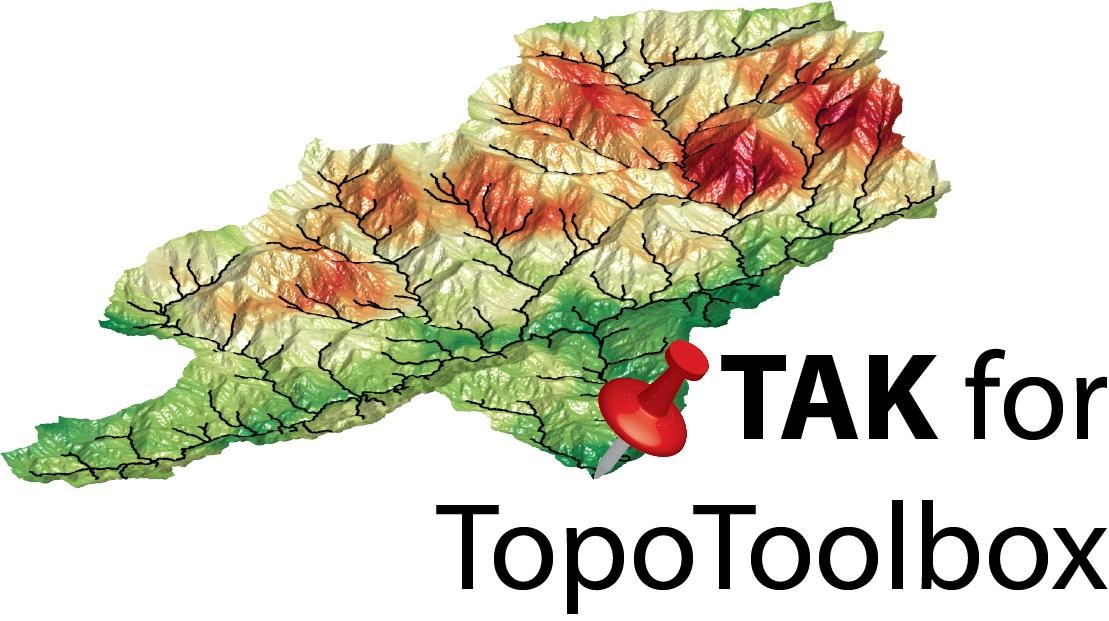
\includegraphics[width=12cm]{PNGs/TAKlogo.png}}

\begin{document}

\maketitle
\tableofcontents
\newpage

\lstset{language=Matlab,%
	basicstyle=\sffamily,% Set code to San Serif
	breaklines=true,%
	morekeywords={matlab2tikz},
	%keywordstyle=\color{blue},%
	keywordstyle=\color{black},%
	morekeywords=[2]{1}, keywordstyle=[2]{\color{black}},
	identifierstyle=\color{black},%
	stringstyle=\color{mylilas},
	commentstyle=\color{mygreen},%
	showstringspaces=false,%without this there will be a symbol in the places where there is a space
	numbers=none,
	%numbers=left,%
	%numberstyle={\tiny \color{black}},% size of the numbers
	%numbersep=9pt, % this defines how far the numbers are from the text
	emph=[1]{for,end,break},emphstyle=[1]\color{red}, %some words to emphasise
	%emph=[2]{word1,word2}, emphstyle=[2]{style},    
}


%%%%%%%%
\section{Attribution} \label{sec:attrb}
\paragraph{}If you use or modify TAK functions for use in a publication, please cite the main TAK publication:

\begin{itemize}
	\item \bibentry{Forte2019}
\end{itemize}

Also, please cite the original TopoToolbox publications as TAK could not function without TopoToolbox:

\begin{itemize}
	\item \bibentry{Schwanghart2010} 
	\item \bibentry{Schwanghart2014}
\end{itemize}

%%%%%%%%
\section{Download and Install} \label{sec:dwnld}

\subsection{Matlab Functions}

\paragraph{}The TAK functions were written (and periodically updated) to work with the most up to date version of TopoToolbox, this can be downloaded from Wolfgang Schwanghart's \href{https://github.com/wschwanghart/topotoolbox}{GitHub page}. The TAK functions are available from Adam Forte's \href{https://github.com/amforte/Topographic-Analysis-Kit}{GitHub page}. Both the TopoToolbox and TAK functions (and all of their subfolders) must be on your matlab path for the functions to work properly.

\paragraph{}The easiest way to use TAK is to just download a copy of the GitHub repository to your computer and work from that. The disadvantage is that to update you need to delete the old version and replace with a complete download of the new version (even if just a single function was updated). To avoid this, a suggested strategy for more advanced users for both the TopoToolbox and TAK functions is to 'fork' copies of these repositories and use these forked versions on your local machine. Periodically, you can \href{https://help.github.com/articles/syncing-a-fork/}{sync your fork} with the master of the original repository to merge in any changes that have been made to either TopoToolbox or TAK. If you are uncomfortable with the command line, this can also be done on the web version of GitHub by 'comparing' branches (for updating TopoToolbox, make sure the 'head fork' is wschwanghart/topotoolbox and the 'base fork' is your forked version of TopoToolbox, follow a similar procedure for TAK), click on the 'Create pull request' button, give the pull request a name in the 'Title' box (the new 'Create pull request' button will be grayed out until you provide a name) click 'Create pull request', click 'Merge pull request', and then finally click 'Confirm merge'. Your forked version will now be up to date with the master of TopoToolbox or TAK.

\subsection{Compiled Functions} \label{sec:CmpFunc}
\paragraph{}In attempt to make these functions accessible to a wider range of users, we have also produced compiled versions of these functions that do not require Matlab to run. Within the main repository, there is a folder called 'Compiled\_Versions' that contains three folders associated with the compiled versions, 'cmpMfiles', 'Windows', and 'MacOSx'. The 'cmpMfiles' folder contains modified versions of all the matlab functions that were compiled, for reference (you will likely need to look at these to understand the inputs to the compiled functions). The compiled versions all have a 'cmp' prefix on them to differentiate them from the main functions (these are all functional in Matlab on their own, though it's not generally recommended that you use these in Matlab over their main counterparts), but as described below, when calling a function from the command line of the compiled TAK, you use the name of the desired function without the 'cmp' prefix. The master function is 'TAK.m' (for which there is not a comparable function in the non-compiled versions). This master function will not successfully run in Matlab as it is designed to translate inputs from the command line to the other functions in a way that works only when used in a deployed (i.e. compiled) mode. The 'Windows' and 'MacOSX' folders each contain an executable named \textit{InstallTAKandMatlabRuntime} (with either an .exe or .app extension depending on the OS). Double clicking this executable will install the Matlab runtime environment that is necessary to run compiled matlab code and the executable for TAK. To keep the size of this install file manageable, this executable needs to access the internet to download the Matlab Runtime. Additionally, you will likely need to have administrator privileges on your local machine in order to successfully install Matlab Runtime. If you have previously installed the Matlab runtime environment, versions of just the TAK executable can be found in the 'Files\_Only' folder. 

\paragraph{}Compiled TAK functions are designed to be run from the command line (i.e. cmd prompt on Windows, terminal on Mac OS X). \textbf{This means that after you have installed the compiled TAK functions, double clicking on the TAK.exe file or a shortcut to it will result in an error indicating that it is missing required arguments. You must run it from the command line as described below!} The procedure for running the compiled TAK functions differs between Windows and Mac OS X and is described in the readme that appears along with the executables. After installing Matlab Runtime, on Windows, open a command prompt and navigate to the location of the TAK executable and then simply call TAK:

\begin{lstlisting}[language=bash]
TAK arguments
\end{lstlisting}

\noindent
The procedure is a little more complicated on Mac OS X, here there is a shell script to run the application but it requires that you specify the location of the Matlab Runtime environment. For example, after installing Matlab Runtime and navigating to the location of the TAK executable and this shell script (with a .sh file extension) in a terminal window:

\begin{lstlisting} [language=bash]
./run_TAK.sh /location/of/runtime arguments
\end{lstlisting}

\noindent
As described in the readme associated with the Mac version, you can avoid having to give the location of the Matlab Runtime environment every time you run TAK by permanently setting the DYLD\_LIBRARY\_PATH location in your path.

\paragraph{}Compiled TAK expects that the first argument (after whatever is required to call the main TAK function depending on the operating system you are using) will be the name of the function you wish to use  and the second argument will be the \textbf{full path} (it really does need to be the full path) to your working directory. TAK expects that all input data that you reference are stored in this working directory and it will store all output data in this working directory (or folders created within this working directory). Generally, the compiled versions of the functions take the same input as the matlab functions described in detail in later sections, but in some cases, because of the limitations of the style of inputs allowed, these inputs are slightly different (e.g. functions require a text file input instead of a cell array input, etc). To understand the inputs to the compiled functions, please refer to the headers of the relevant codes stored in the cmpMfiles folder and Section \ref{sec:CmpFuncCalls} of the Appendix. 

\paragraph{}It is important to note that the form of inputs are also different at the command line. In short, no input should be included in quotes regardless of the input type and each input should be separated by a single space. For example to call the compiled version of \nameref{sec:MakeStreams} on Mac OS X:

\begin{lstlisting}[language=bash]
./run_TAK.sh /location/of/runtime MakeStreams /location/of/working/directory dem.tif 1e6 topo_files no_data_exp auto
\end{lstlisting}

\noindent
where 'MakeStreams' is the name of the function you want to use, '/location/of/working/directory' is the working directory where input data will be read from and output data will be stored, 'dem.tif' is the first required input of MakeStreams and is the name of the dem file to import, '1e6' is the second required input of MakeStreams and is the threshold accumulation area to use, 'topo\_files' is the third required input of MakeStreams and is the name for output files (note that this is NOT a required input for the standard Matlab version of MakeStreams), 'no\_data\_exp' is the name of an optional parameter for MakeStreams, and 'auto' is the value being passed to that optional parameter. Some standards for the inputs; 1)  when the function requires that you provide a name of an input file, it expects that the file includes the file extension (e.g. .txt, .mat, .shp, etc) because it will use this file extension to make sure you're providing the correct kind of file, 2) any text file input is expected to have a .txt extension, 3) theoretically comma or tab delimited data are both fine for text file inputs, but in practice, comma delimited files are preferred, and 4) when the function requires (or allows as an optional input) the name of an output file, DO NOT include a file extension as this name will likely be used for several different files with different extensions and the function will handle appending the proper file extensions. The header of 'cmp*.m' files for each function contain example inputs to the command line to run that function.

\paragraph{}The compiled versions are designed to mostly behave exactly the same as the non-compiled functions running Matlab with a few minor exceptions (e.g. the compiled versions of \nameref{sec:KsnProfiler} and \nameref{sec:BsnPckr} do not allow for you to zoom into a location on the DEM before you start picking). All function names described in later sections are valid functions to invoke in the compiled version of TAK except \textit{ksncolor}, \textit{CatPoly2GRIDobj}, or \textit{ProjectOntoSwath}. Also note that two functions exist in compiled TAK which do not exist in the regular Matlab version. These functions, called as \textit{PrepareAddGrids} and \textit{PrepareCatAddGrids} at the command lines, are designed to prepare inputs for additional grids and additional categorical grids, respectively, for use in the compiled version of \nameref{sec:PrcRvBsn}. Refer to the 'cmp' files for these two functions ('cmpPrepareAddGrids.m' and 'cmpPrepareCatAddGrids.m') for instructions for use. 

\section{Error Reporting}
\paragraph{}We have tried to ensure that all options work properly within both the Matlab and compiled versions of TAK, but unexpected errors may occur. The preferred method of error reporting is to use the built in \href{https://github.com/amforte/Topographic-Analysis-Kit/issues}{'Issues'} function on the GitHub page for TAK so that there is a record of user encountered errors. If you have forked a version of the code and think you can fix an error, issue a pull request with the change, collaboration is welcome! If all else fails, you can email \href{mailto:aforte8@lsu.edu}{Adam Forte} as well. Before submitting an issue or contacting Adam, please check both open and closed issues to see if the bug has already been reported or fixed in an updated version. Whether submitting an issue or emailing Adam, please provide as much information as possible on the error (e.g. cut and paste the error message you received) and what you were doing when it occurred.

%%%%%%%%
\section{Preparing Datasets for TAK} \label{sec:exmpl}
\paragraph{}TopoToolbox and TAK functions are designed assuming that data is supplied to them are in a projected coordinate system with meters as linear units (e.g. UTM ) with square pixels (i.e. dx = dy) and will produce unexpected results (or may error out) if you do not reproject your data into a suitable projection and coordinate system. Similarly, for functions that take multiple datasets as inputs (e.g. \nameref{sec:PrcRvBsn}) it is expected that all of the datasets you provide are in the same projection system. We would generally recommend doing the reprojections in a GIS environment (e.g. ArcGIS, QGIS, GDAL, etc), but TopoToolbox does include some functions to reproject data (e.g. \textit{reproject2utm}, \textit{projectGRIDobj}).

\paragraph{}TAK relies on either TopoToolbox or Matlab functions for importing geographic data and thus is limited to the data types supported by these. Specifically, for raster data (e.g. digital elevation models, other gridded data), TAK can interpret and/or export data that are GeoTiffs or ESRI ArcGIS ASCII files (both of which are readable by a variety of GIS programs including ArcGIS, QGIS, and GDAL). For importing or exporting vector data, TAK uses shapefiles (which are again readable and writable by a variety of GIS programs including ArcGIS, QGIS, or OGR).

\paragraph{}It's important to note that projected data (e.g. geotiffs, ascii grids, shapefiles, etc) exported from Matlab will not include georeferencing information. The data is still projected (in the same projection as the original input data), but you will need to define the projection in the GIS program you are using.

\paragraph{}In this this manual, we use an example dataset from Southern California to demonstrate outputs of some of the functions included as part of TAK (Figure \ref{fig:Topo}). The example data is available within the released version of the TAK code on GitHub and is contained within a tarball called \textit{'ExampleData.tar.gz'}. Within this tarball, you'll find:

\begin{itemize}
	\item \textit{SoCal\_UTM\_DEM.tif} - GeoTiff of the example data area shown in Figure \ref{fig:Topo} from \href{http://opentopography.org/}{Open Topography} and reprojected into UTM 11N
	\item \textit{prism\_precip.tif} - GeoTiff of 30 year normals of precipitation from \href{http://www.prism.oregonstate.edu/normals/}{PRISM}, data was cropped and reprojected into UTM 11N
	\item \textit{geo\_polygons.shp} - Polygon shapefile of Geology of California from \href{https://maps.conservation.ca.gov/cgs/#datalist}{California Department of Conservation}, data was reprojected into UTM 11N
	\item \textit{river\_mouths.txt} - text file containing the river mouths used to generate basins in the example using \nameref{sec:PrcRvBsn}
\end{itemize} 

\begin{figure}[H]
	\includegraphics[width=16.5cm]{PNGs/Topo.png}
	\caption{Example dataset area used in this manual.}
	\label{fig:Topo}
\end{figure}

\paragraph{}Matlab, and thus TopoToolbox and TAK, generally require that an entire dataset be loaded into active memory before it can be used. This means that the size of DEM you can successfully process and use in TAK will be dependent on the available memory (i.e. RAM) of the computer on which you're running TAK along with the operating system (Mac OS X, Windows, and Linux versions of Matlab deal with memory in slightly different ways). It's also not as straightforward as looking at the size of the input DEM as you need to account for all the datasets that need to be in active memory for many TAK functions, e.g. a GRIDobj, a FLOWobj, and a STREAMobj. If you are encountering memory issues, there aren't too many simple solutions, but the best bets are to either spit your data into smaller segments (though you must be careful to not introduce errors by truncating portions of drainage basins of interest) or use a dataset with a larger cellsize. 

%%%%%%%%
\section{Workflow} \label{sec:workflow}

\paragraph{}Possible workflows through the functions provided as a part of TAK are outlined in Figure \ref{fig:Workflow}. In the sections that follow, descriptions of each function are provided and in some cases, possible outputs are included as figures using the example dataset. In later sections we assume that you have a basic familiarity with Matlab data types (e.g. arrays, cell arrays, structures, tables, etc) and the four main TopoToolbox classes (i.e. \textit{GRIDobj}, \textit{FLOWobj}, \textit{STREAMobj}, and \textit{SWATHobj}), but we provide a brief primer in Section \ref{sec:primer}. This manual does not include all options for all functions; we refer users to the headers of each relevant function for a complete list of required and optional parameters. Instead, this manual is designed to highlight the basic utility of the functions along with some underlying rationale / methodology employed within some of the functions and to provide examples of some recommended use cases.

\begin{figure}[H]
	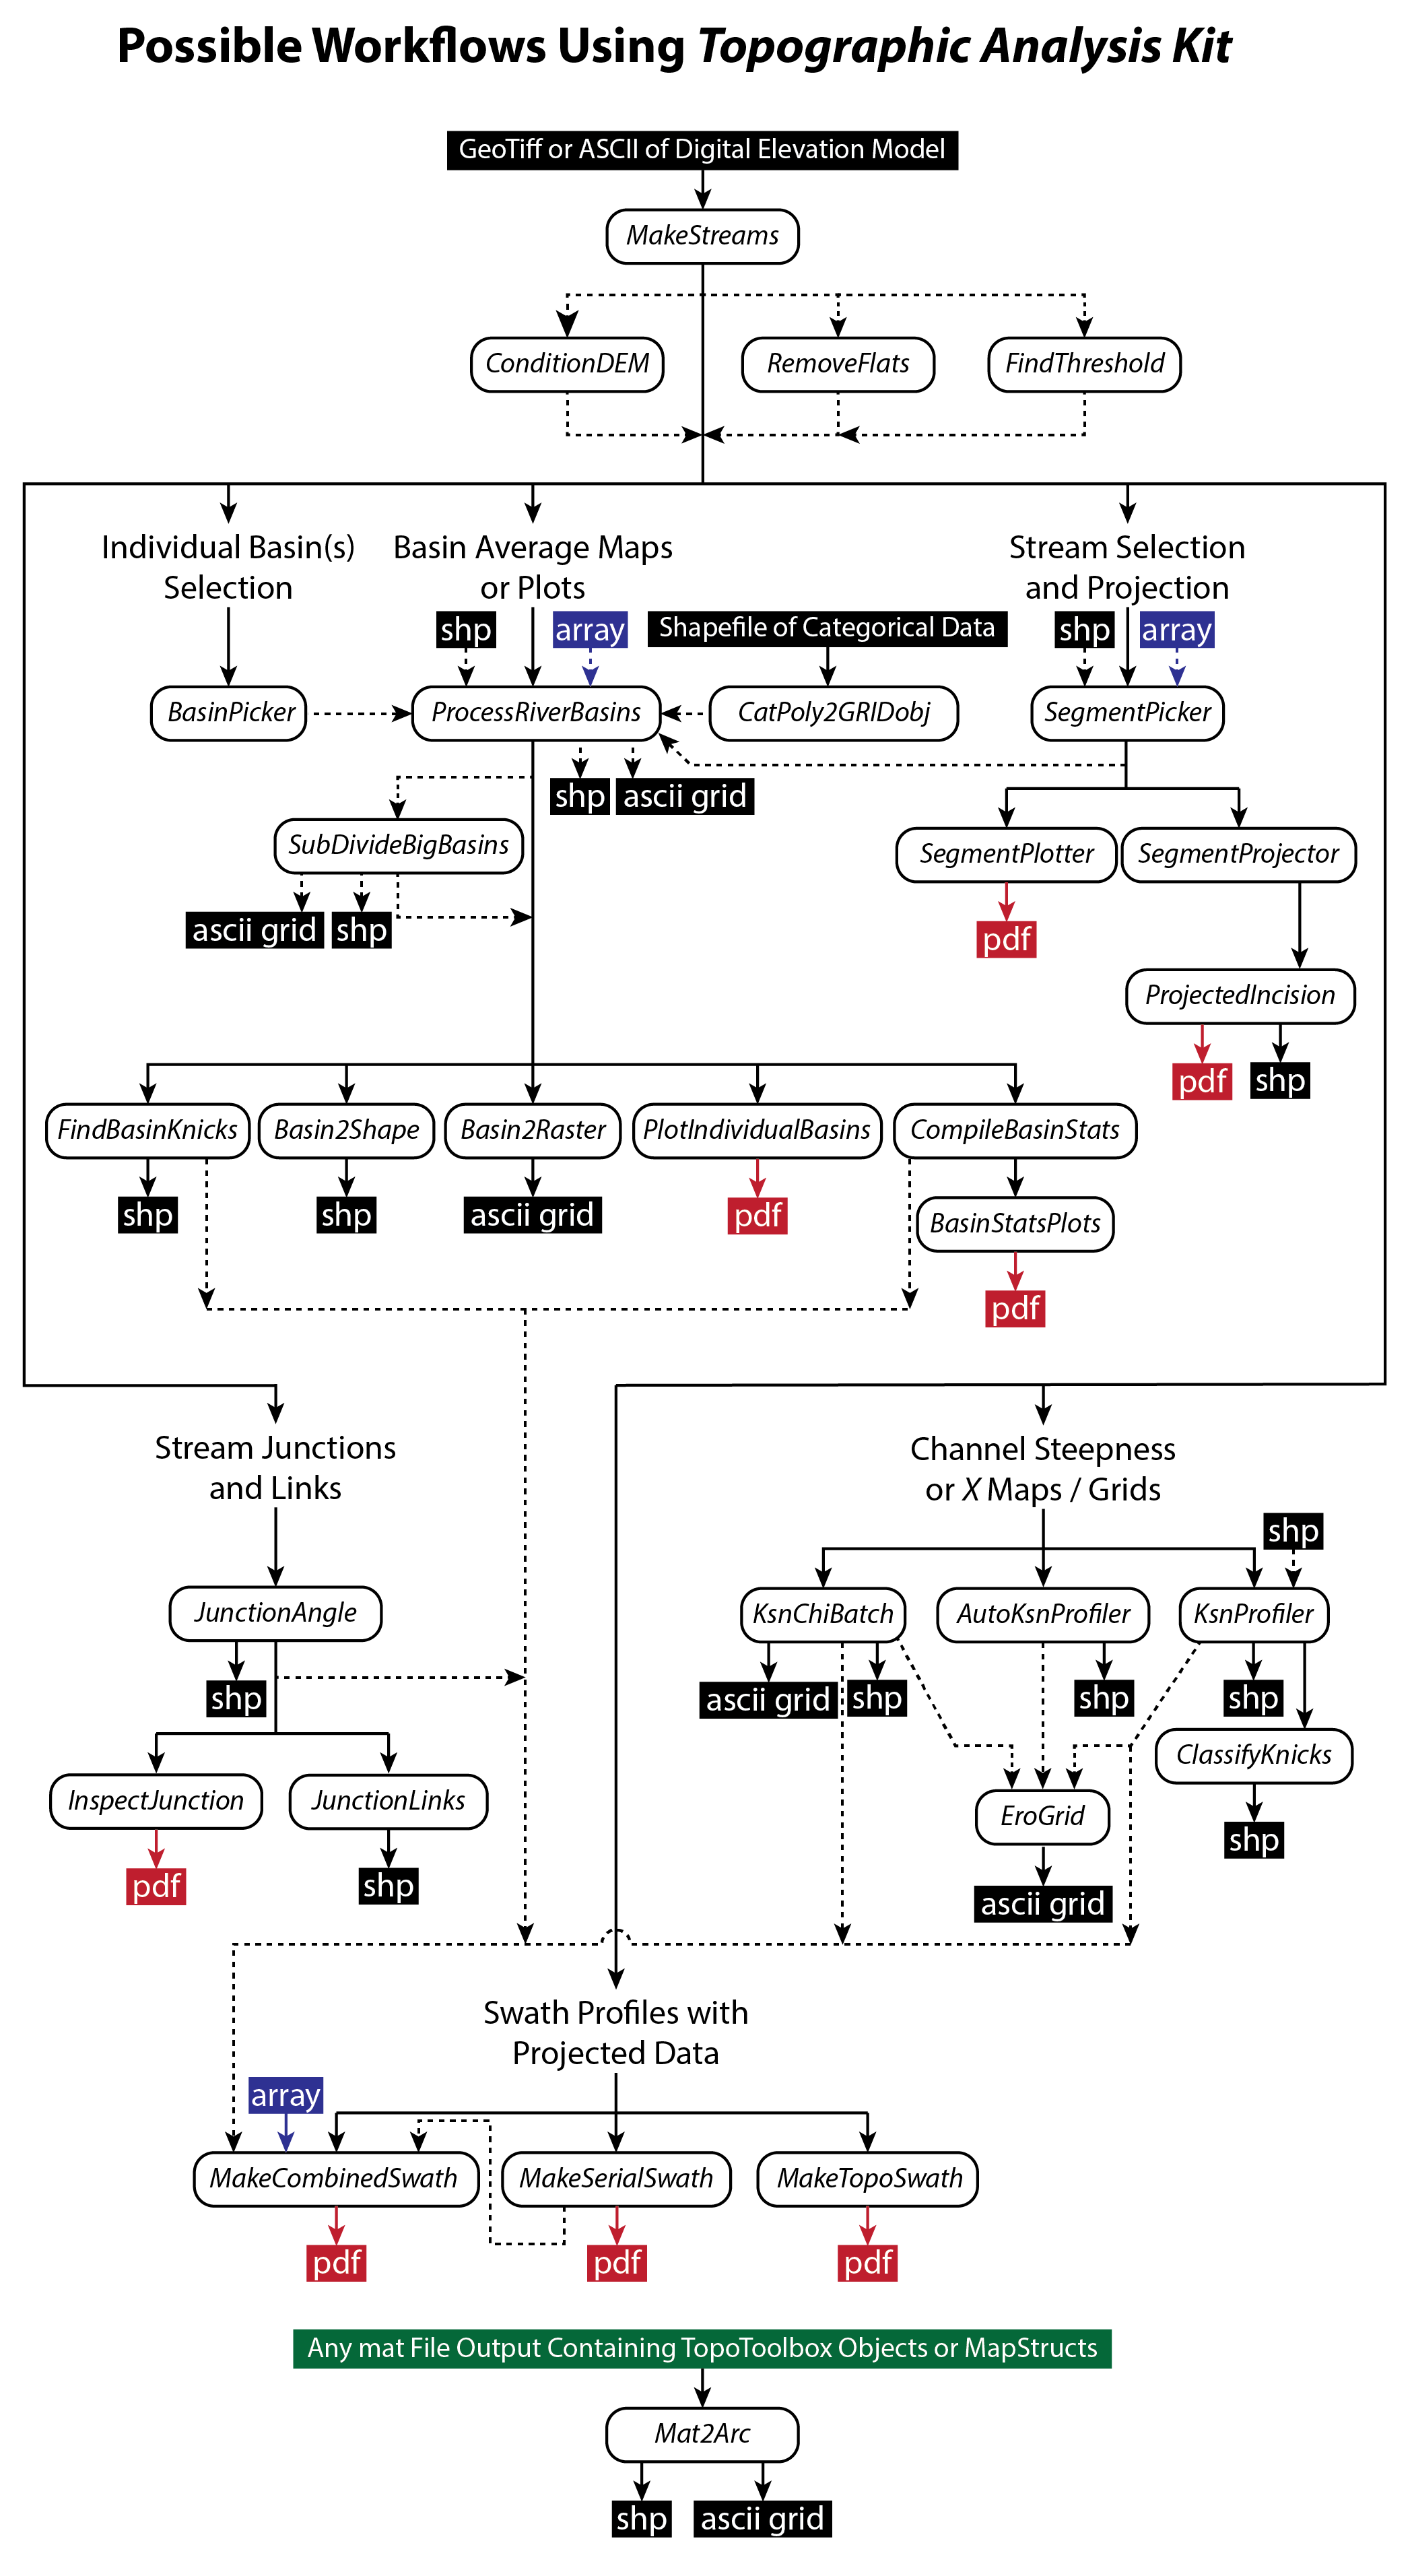
\includegraphics[width=16.5cm]{PNGs/FlowChart.png}
	\caption{Suggested workflows through TAK functions depending on desired outcome and purpose of analysis. Also highlighted are the nature of the outputs produced by different functions. Definitions of inputs and outputs: shp - a shapefile containing vector data, the geometry of which, e.g. points, lines, polygons, depends on the tool in question; array - a Matlab array, i.e. a matrix of numbers; ascii grid - an ESRI Ascii text file that is interpretable as gridded raster data with projection information by many GIS programs; pdf - a figure output as a PDF.}
	\label{fig:Workflow}
\end{figure}

%%%%%%%%
\section{Matlab and TopoToolbox Crash Course} \label{sec:primer}
\paragraph{}The following sections are written for people who have never used Matlab (Sections \ref{sec:dataPrimer}, \ref{sec:funcPrimer}, \ref{sec:loadPrimer}) or TopoToolbox (Section \ref{sec:ttPrimer}). If you are familiar with basic manipulations of Matlab datatypes,  general procedure for using Matlab functions, how to load and save variables in matfiles, and the four primary TopoToolbox classes, feel free to skip these sections and get right into \nameref{sec:idp} with TAK.

\subsection{Matlab Data Types} \label{sec:dataPrimer}
\paragraph{}There are four Matlab data types that appear commonly in TAK functions as either inputs or ouptuts (in addition to TopoToolbox specific classes, described in section \ref{sec:ttPrimer}), arrays, cell arrays, tables, and structures/geographic data structures.

\subsubsection{Arrays}
\paragraph{}Arrays are the most basic data type in Matlab and are essentially a matrix of numeric values. They have some specific rules associated with them, most importantly that they can only contain numbers and that there can be no empty elements in an array:

\begin{lstlisting}[language=Matlab]
% To make an array, values separated by semicolons indicate rows and values separated by commas indicate columns, and encasing them in brackets indicates that it is an array, so
a=[1;2;3];
% Will make an array with 3 rows and 1 column, whereas
a=[1,2,3];
% Will make an array with 1 row and 3 columns, and
a=[1,2,3;4,5,6];
% Will make an array with 2 rows and 3 columns
% The semicolon at the end of the previous commands suppresses any output to the command prompt
% Positions within a matlab array can be specified by their row and column position (note that the first index in Matlab is 1, not 0 like in C, Java, Python, etc), so calling
a(1,2)
% Will print 2 at the command prompt as this is the number in the first row and second column.
% Positions can also be specified by their 'linear index', which is a single number that starts counting from position (1,1) and proceeds down columns and then across rows, so
a(5) 
% Will print 5 at the command prompt, this is equivalent to calling a(1,3)
\end{lstlisting}

\subsubsection{Cell Arrays}
\paragraph{}Cell arrays are versatile data types that can be thought of as an array of containers. Cell arrays are primarily used in TAK in \nameref{sec:PrcRvBsn}. Each 'cell' in a cell array can contain pretty much any other data type, e.g. a single number, and entire array, another cell array, etc:

\begin{lstlisting}[language=Matlab]
% Making a cell array is similar to making an array, except you use curly brackets instead of square brackets
c={1,2,3};
% Will produce a 1 x 3 cell array
% Cell arrays can contain different types of data with different dimensions in each cell
a=[1,2,3;4,5,6];
c={a,5,'cells can contain strings too'};
% Will also produce a 1 x 3 cell array but this time with very different data stored in each cell
% To reference a particular cell, you need to use curly brackets again
c{1,2}
% Would print 5 to the comman prompt, where as
c{1}
% Would print the entire array stored in a to the command prompt
% You can also use parantheses to index a cell array, but in this case the result is a new cell array just containing the cells you specified
new_c=c(2);
% Would produce a 1 x 1 cell array containing the number 5 in the cell, whereas
new_c=c(1,2:3);
% Would produce a 1 x 2 cell array with the number 5 in the first cell, and the string 'cells can contain strings too' in the second cell
\end{lstlisting}

\paragraph{}There are some useful functions to be aware of for converting between arrays and cell arrays, specifically \textit{mat2cell}, \textit{cell2mat}, and \textit{num2cell}. These may be useful in preparing inputs for TAK functions, so we would suggest looking at the help files on these functions if you are having problems generating some of the required inputs for particular TAK functions.

\subsubsection{Tables}
\paragraph{}Tables are similar to cell arrays in that elements within a table can contain a variety of different types of data, but they differ primarily in that they also allow you to specify column and row names and thus the way you access data within tables is different. Tables are primarily used in TAK in the \nameref{sec:CompStats}, \nameref{sec:CatGrid}, and \nameref{sec:BSPlots} functions. As an example, consider extracting information from the table output from \nameref{sec:CombSwath}:

\begin{lstlisting}[language=Matlab]
% You can querry the size of a table with size
size(T)
% The entire contents of a particular column can be stored as a new variable by calling the name of the table, e.g. to extract the contents of the 'mean_ksn' column which contains basin averaged normalized channel steepness data in the table output from the CompileBasinStats
all_ksn=T.mean_ksn;
% You can also extract the contents of a single element within a column, e.g., to extract the 10th element of the 'mean_ksn' column
ksn10=T.mean_ksn(10,1);
% Individual elements in a table can contain data of variable sizes and types, e.g. in the table output from CompileBasinStats, each element of the 'mean_ksn' column will have one numeric value, where as each element of the 'hyps' column will have a n x 2 array containing the hypsometry information for a particular basin
\end{lstlisting}


\paragraph{} Tables can also be a useful way to load in data for use in other functions, though generally you will need to convert to other Matlab data types to be valid input for TAK functions:

\begin{lstlisting}[language=Matlab]
% To read in a file containing mixed data, e.g. a text file with columns named 'sample_names', 'sample_lat', and 'sample_lon' and containing the names of samples as characters, the latitude of samples, and the longitude of samples respectively
T=readtable('samples.txt');
% Particular columns can be easily extracted to arrays or cell arrays
lat=T.sample_lat; % Will produce an array named lat
lon=T.sample_lon; % Will produce an array named lon
samples=T.sample_names; % Will produce a cell array named samples because the sample_names column contains characters
% You can also reference particular rows of particular columns, for columns containing numbers you reference these like arrays, for columns containing characters you reference these like cell arrays
% Grabbing the 10th row of each column
lat10=T.sample_lat(10,1);
lon10=T.sample_lon(10,1);
name10=T.sample_names{10,1};
\end{lstlisting}

\subsubsection{Structures}
\paragraph{}Structures allow you to group similar data and store them in containers referred to as fields. Structures can also have multiple dimensions like an array. In TAK, structures are used within the context of geographic data structures, which are a special subset of structures that contain specific fields and can be written out as shapefiles using the \textit{shapewrite} command. Geographic data structures must have fields named, Geometry, X and Y (or Lon and Lat), and BoundingBox (unless the Geometry is Point). We refer interested readers to the Matlab Help documents for the specific requirements of the data stored in these fields if you wish to generate a valid geographic data structure that can be output as a shapefile on your own. Geographic information structures can also have additional fields which will be interpreted as fields in the output shapefile. Several functions produce geographic data structures, e.g. \nameref{sec:PrcRvBsn} or \nameref{sec:KsnBatch}. Consider the example of interacting with the \textit{'MSNc'} geographic information structure stored within the outputs of \nameref{sec:PrcRvBsn} that contains information related to \textit{k\textsubscript{sn}}:

\begin{lstlisting}[language=Matlab]
% You can querry the dimensions of a structure with size
size(MSNc)
% Which in the case of 'MSNc' will be n x 1 depending on the size of the stream network
% You can also querry which fields are stored in 'MSNc' with fieldnames
fieldnames(MSNc)
% You can extract the contents of a given field from a particular dimension, for example to extract what's stored in the 'ksn' field in the 10th element
ksn10=MSNc(10,1).ksn;
% Examining these fields, you can see that they have variable sizes, for example the 'Geometry' field has a single entry per element that is 'Line', indicating that the shapefile Geometry type is Line, where as the X and Y fields will have n x 1 arrays specifying the X and Y coordinates of line segments
% You may wish to extract all the values from a specific field, e.g. all the normalized steepness values stored in the ksn field, but unlike with a table if you simply call a field without specifying a dimension, you will get the first element, not the entire list of elements
MSNc.ksn % Will print whatever ksn value is in the MSNc(1,1).ksn
% To extract all the ksn values stored in the ksn field, you must concatenate the field values
all_ksn=[MSNc.ksn] % will produce a row vector, 1 x m of ksn values
all_ksn=horzcat(MSNc.ksn) % will produce a row vector, 1 x m of ksn values
all_ksn=vertcat(MSNc.ksn) % will produce a column vector n x 1 of ksn values
% Valid geographic information structures can be output as shapefiles
shapewrite(MSNc,'ksn.shp');
% You can also import shapefiles into Matlab as geographic information structures
MS=shaperead('shape_name.shp');
\end{lstlisting}

\subsection{Using Matlab Functions} \label{sec:funcPrimer}
\paragraph{}All of the files included in TAK are written as Matlab functions. A Matlab function is stored in a '.m' file and is called by the name of that file:

\begin{lstlisting}[language=Matlab]
% For a function file named TestFunction.m, you would call it like this at the command prompt in Matlab
TestFunction(my_array);
% In this example, the TestFunction has one input that is an array
\end{lstlisting}

\noindent
All of the TAK functions have extensive 'headers', i.e. commented text that appears at the top of the .m file that contains a description of the use of the function along with lists of inputs and outputs. You can always open an .m file in Matlab or a text editor to view these, but you can also access them directly from the command line:

\begin{lstlisting}[language=Matlab]
% Starting the call for a function like this
TestFunction(
% Will display a pop up showing the required inputs for the function and inclue a link labeled 'More Help...' that if clicked will open the header information for the function in a new window.
\end{lstlisting}

\paragraph{}The majority of TAK functions have both required and optional inputs. As the names imply, required inputs are data or information the function must have to run, where as optional inputs are inputs that can be omitted and the function will still run.If you open a '.m' file in a text editor or the Matlab editor, the first line, which defines how the function is called, will list the required inputs, e.g.:

\begin{lstlisting}[language=Matlab]
% A function definition with one required input
function TestFunction(my_array)
\end{lstlisting}

\noindent
If there optional inputs, there will simply be an apparent input named 'varargin', meaning that the function is capable of accepting variable arguments:

\begin{lstlisting}[language=Matlab]
% A function definition with one required input and an arbitrary number of optional inputs
function TestFunction(my_array,varargin)
\end{lstlisting}

\noindent 
In many cases, values for optional inputs are required for the function to run, but they have a default value that will be used if the user does not supply a value to the optional input (e.g. many TAK functions require a reference concavity, this is always specified as an optional parameter that will be set to 0.5 if you do not provide a different number). Required inputs for TAK functions will generally will take one of three forms: 

\begin{enumerate}
	\item The name of a variable stored in the workspace
\begin{lstlisting}[language=Matlab]
% The header of TestFunction tells you that it has one required input that is a Matlab array named INPUT, this means you can provide any Matlab array (with any name) to TestFunction
TestFunction(my_array);
% Alternatively, if TestFunction says it requires two inputs, INPUT1 and INPUT2, i.e. the help pop up looks like TestFunction(INPUT1,INPUT2), and the first input is supposed to be a Matlab array and the second is supposed to be a Matlab cell array, then a valid input would be
TestFunction(my_array,my_cell_array);
% Always consult the header for specific requirements, some arrays have restrictions on their dimensions, e.g. they must be an n x 2 array. Inputs to TAK functions will be 'parsed' so if they do not meet the requirements, you will be informed of this and the function will error out
\end{lstlisting}	
	\item A character string defining an option or giving the name of a file or folder
\begin{lstlisting}[language=Matlab]
% The header of TestFunction tells you it requires one input Method that defines a method and that the valid inputs to method are 'split' or 'join', so
TestFunction('split');
% Would be a valid call to the function, where as
TestFunction(split)
% Would not be a valid call
% Similarly, if a required input is the name of a file, you would give these in single quotes 
TestFunction('my_file.txt');
\end{lstlisting}
	\item A logical value
\begin{lstlisting}[language=Matlab]
% The header of TestFunction tells you that it has one required input, Do_X and that this expects a logical value, then you could call it like this
TestFunction(true);
% Or like this
TestFunction(1);
% As 0 and 1 are equivalent to false and true, respectively
\end{lstlisting}	
	
\end{enumerate}

\paragraph{}Optional inputs follow many of the same rules, but they importantly differ in that they require that they are proceeded by the name of the optional parameter:

\begin{lstlisting}[language=Matlab]
% From the header of TestFunction, you learn that it has three required inputs, 1) data, which expects a Matlab array, 2) method, which specifies a method to use on the data that is either 'split' or 'join', and 3) save_output, which expects a logical value. TestFunction also has two optional parameters, 1) file_name, which expects the name of the file to be output and 2) extra_data, which expects another Matlab array. All of the following are valid calls to TestFunction
TestFunction(my_array,'split',true); % Running function with no optional inputs
TestFunction(my_array,'join',true,'file_name','my_file.txt');
TestFunction(my_array,'split',false,'extra_data',my_other_array);
TestFunction(my_array,'join',true,'extra_data',my_other_array,'file_name','my_file.txt');
% Note that the order in which you specify optional parameters doesn't matter, but the argument passed to an optional parameter must always immediately follow the name of the appropriate optional parameter
\end{lstlisting}

\paragraph{}Many of the TAK functions also have outputs that will be stored as variables in the Matlab workspace after a successful run of the function. Outputs are specified like so:

\begin{lstlisting}[language=Matlab]
% The header indicates that TestFunction from the previous example has two outputs, split_data and joined_data, you can specify the name of the variables for these outputs
[my_splits,my_joins]=TestFunction(my_array,'split',true);
% Now variables my_splits and my_joins will appear in your Matlab workspace
% If you don't actually care about one of the outputs, e.g. you only want my_joins, you can supply a ~ to any output you don't want to be output to the workspace
[~,my_joins]=TestFunction(my_array,'split',true);
\end{lstlisting}

\subsection{Loading and Outputting Data} \label{sec:loadPrimer}
\paragraph{}The outputs of many TAK functions are automatically saved as 'matfiles', which are versatile matlab files that can contain multiple variables and will have a '.mat' suffix. Some basic operations with matfiles:

\begin{lstlisting}[language=Matlab]
% You can querry the contents of a matfile
whos('-file','Basin_1_Data.mat')
% Which will print out the list of variable names, their sizes, and the type of data stored in that variable to the workspace
% Alternatively, highlighting a matfile in the 'Current Folder' window will display the contents in the bottom left of the Matlab screen
% If you want to load in a particular variable, you can use load
load('Basin_1_Data.mat','DEMcc'); % Will load the DEMcc variable into the workspace
% You can load all variables contained in a matfile by not specifying any variables with the load command
load('Basin_1_Data.mat');
% The syntax for saving data into a matfile is similar
save('MyMat.mat','DEMcc');
% If the specified mat file name already exists, the previous action will overwrite the matfile. If you instead want to add the variable to the variables already stored in the matfile, you can use '-append'
save('MyMat.mat','DEMcc','-append');
\end{lstlisting}


\subsection{TopoToolbox Classes} \label{sec:ttPrimer}
\paragraph{}There are four primary TopoToolbox classes, \textit{GRIDobj}, \textit{FLOWobj}, \textit{STREAMobj}, and \textit{SWATHobj}. We refer interested users to the TopoToolbox documentation or \href{https://topotoolbox.wordpress.com/}{Wolfgang Schwanghart's excellent blog} for detailed discussions of these data classes, but below we provide a very brief description of these different classes. A general point to be aware of when using TopoToolbox classes is that many functions require several of these different classes and, unless otherwise stated, it is assumed that these are datasets that were generated together and from each other (e.g. the \textit{STREAMobj} generated from a particular \textit{FLOWobj} which in turn was generated from a particular \textit{GRIDobj}). You generally don't need to worry about this if you are using the TAK functions exclusively, but if you ever get an error regarding datasets not aligning, check to make sure you are not mixing different TopoToolbox datasets that did not derive from the same DEM. 

\paragraph{}The TopoToolbox dataclasses are unique, but in terms of other Matlab data types, they are the most similar to a 1 dimensional structure, i.e. they contain a series of 'fields' that contain a variety of different data types:

\begin{lstlisting}[language=Matlab]
% To extract the data array within a GRIDobj named DEM
elevations=DEM.Z; % Will be a n x m array of numeric values
% To extract the cellsize of a GRIDobj named DEM
cellsize=DEM.cellsize; % Will be a single value
% The contents of a TopoToolbox object can be querried with the 'fieldnames' function, just like a structure
fieldnames(DEM)
% Will output a cell array with the names of the fields contained within DEM
\end{lstlisting}

\subsubsection{\textit{GRIDobj}}
\paragraph{}\textit{GRIDobj}s are for storing raster data. In TAK, they are how DEMs, flow accumulation rasters, and other additional gridded data is stored. It is very simple to generate a \textit{GRIDobj}:

\begin{lstlisting}[language=Matlab]
% GRIDobjs can be created from ascii grids or geotiffs
DEM=GRIDobj('/path/to/gridded__elevation_data.txt');
GRID=GRIDobj('/path/to/other_gridded_data.tif');
\end{lstlisting}

\noindent
It is important to note that it is recommended that you project data into a projected coordinate system (e.g. UTM) before turning it into a GRIDobj, failure to do so will result in errors in various TAK functions.

\noindent
If you want to plot a \textit{GRIDobj}

\begin{lstlisting}[language=Matlab]
% To plot a single GRIDobj
imagesc(GRID);
% To plot a hillshade colored by another GRIDobj (can provide the DEM as the second input to color by elevation)
imageschs(DEM,GRID);
\end{lstlisting}

\subsubsection{\textit{FLOWobj}}
\paragraph{}\textit{FLOWobj}s are special data classes for storing flow routing information. Unlike a flow direction raster in ArcGIS, this is not something that can be easily visualized, but it is a crucial dataset used for almost all TAK functions. 

\subsubsection{\textit{STREAMobj}}
\paragraph{}\textit{STREAMobj}s are data classes for storing stream networks. To plot a \textit{STREAMobj},

\begin{lstlisting}[language=Matlab]
%To plot a map of a STREAMobj
plot(S);
% To plot a longitudinal profile of the streams in a STREAMobj
plotdz(S,DEM);
\end{lstlisting}

\subsubsection{\textit{SWATHobj}}
\paragraph{}\textit{SWATHobj}s are data classes for storing swath data extracted from \textit{GRIDobj}. To create a basic plot of a \textit{SWATHobj},

\begin{lstlisting}[language=Matlab]
%To plot swath profile of a SWATHobj 
plotdz(SW);
\end{lstlisting}

%%%%%%%%
\section{Initial Data Processing} \label{sec:idp}

\subsection{\textit{CheckTAKDependencies}} \label{sec:Depend}
\paragraph{}TopoToolbox and TAK require several different Matlab toolboxes. \textit{CheckTAKDependencies} is a simple function that checks to see if you have licensed versions of all the required toolboxes. 

\begin{lstlisting}[language=Matlab]
% CheckTAKDependencies takes no inputs and has no formal outputs
% If running 
CheckTAKDependencies
% Produces no warnings, then all of the TAK functions should work (or at least, they shouldn't fail because of missing dependencies!)
% Alternatively you may see text like:
'Warning: Fatal error: You do not have a license for the Mapping Toolbox, TopoToolbox will not function properly'
% If you are missing a crucial TopoToolbox, or this:
'Warning: You do not have a license for the Statistics and Machine Learning Toolbox, some functions will not work properly'
% If you are missing a Toolbox that are only used by some TAK functions
\end{lstlisting}

\noindent
TAK requires licenses for the Image Processing Toolbox, Mapping Toolbox, Optimization Toolbox, and Statistics and Machine Learning Toolbox. If you do not have all licenses for all of these, you may need to use the \nameref{sec:CmpFunc}.

\subsection{\textit{MakeStreams}} \label{sec:MakeStreams}
\paragraph{}\textit{MakeStreams} is a simple wrapper around creating the basic TopoToolbox objects needed for the majority of other TAK functions, specifically a digital elevation model (DEM) as a \textit{GRIDobj}, a flow direction dataset as a \textit{FLOWobj}, a flow accumulation grid as a \textit{GRIDobj}, and a stream network as a \textit{STREAMobj}. It should be noted that while, as described in more detail in \cite{Schwanghart2014}, TopoToolbox supports flow routing using either D8 or D$\infty$ algorithms, TAK functions use the simpler D8 flow routing scheme. The minimum inputs to \textit{MakeStreams} are the location of a valid DEM as either a geotiff or ascii grid and a minimum threshold drainage area (in square map units) for beginning stream network definition:
	
\begin{lstlisting}[language=Matlab]
[DEM,FD,A,S]=MakeStreams('/Users/aforte/GISdata/SoCal_UTM_DEM.txt',1e6);
\end{lstlisting}

\paragraph{}The basic usage of \textit{MakeStreams} will produce stream networks, that depending on the nature of your DEM, may include areas that are not of interest or should not be included in stream definition (Figure \ref{fig:AllStreams}).

\begin{figure}[H]
	\includegraphics[width=16.5cm]{PNGs/AllStreams.png}
	\caption{Result of running \nameref{sec:MakeStreams} without any control for flat areas.}
	\label{fig:AllStreams}
\end{figure}

\paragraph{}\textit{MakeStreams} includes various simple options to filter the input DEM. This can be done through a logical expression, for example, if you wanted to set any portions of the DEM at or below 0 m elevation to no data (and thus suppress stream definition), you could use the following:

\begin{lstlisting}[language=Matlab]
[DEM,FD,A,S]=MakeStreams('/Users/aforte/GISdata/SoCal_UTM_DEM.txt',1e6,'no_data_exp','DEM<=0');
\end{lstlisting}

\noindent
There is also a built in auto filter that will identify true flats (i.e. areas of constant elevation) and set these to no data:

\begin{lstlisting}[language=Matlab]
[DEM,FD,A,S]=MakeStreams('/Users/aforte/GISdata/SoCal_UTM_DEM.txt',1e6,'no_data_exp','auto');
\end{lstlisting}



\begin{figure}[H]
	\includegraphics[width=16.5cm]{PNGs/NoFlatsStreams2.png}
	\caption{Result of running \nameref{sec:MakeStreams} with auto removal of flat areas and \textit{min\_flat\_area} set to 1e8.}
	\label{fig:NoFlatsStreams}
\end{figure}

\noindent
Using this auto filter produces a more reasonable stream network and removes the Pacific Ocean and Salton Sea from the areas where streams are defined. (Figure \ref{fig:NoFlatsStreams}). The auto filter considers an area 'flat' if the log of the gradient is undefined and then looks for connected pixels that are identified as 'flat.' The number of connected pixels which will subsequently be treated as a flat area, and set to 'NaN' in the resulting DEM, is controlled by setting a minimum area with the \textit{'min\_flat\_area'} in m\textsuperscript{2}. This is set to a default minimum area of 1e8 m\textsuperscript{2}. Setting this minimum flat area to small values may result in a discontinuous stream network (Figure \ref{fig:min_flat}).

\begin{figure}[H]
	\centering
	\begin{subfigure}{.40\textwidth}
		\centering
		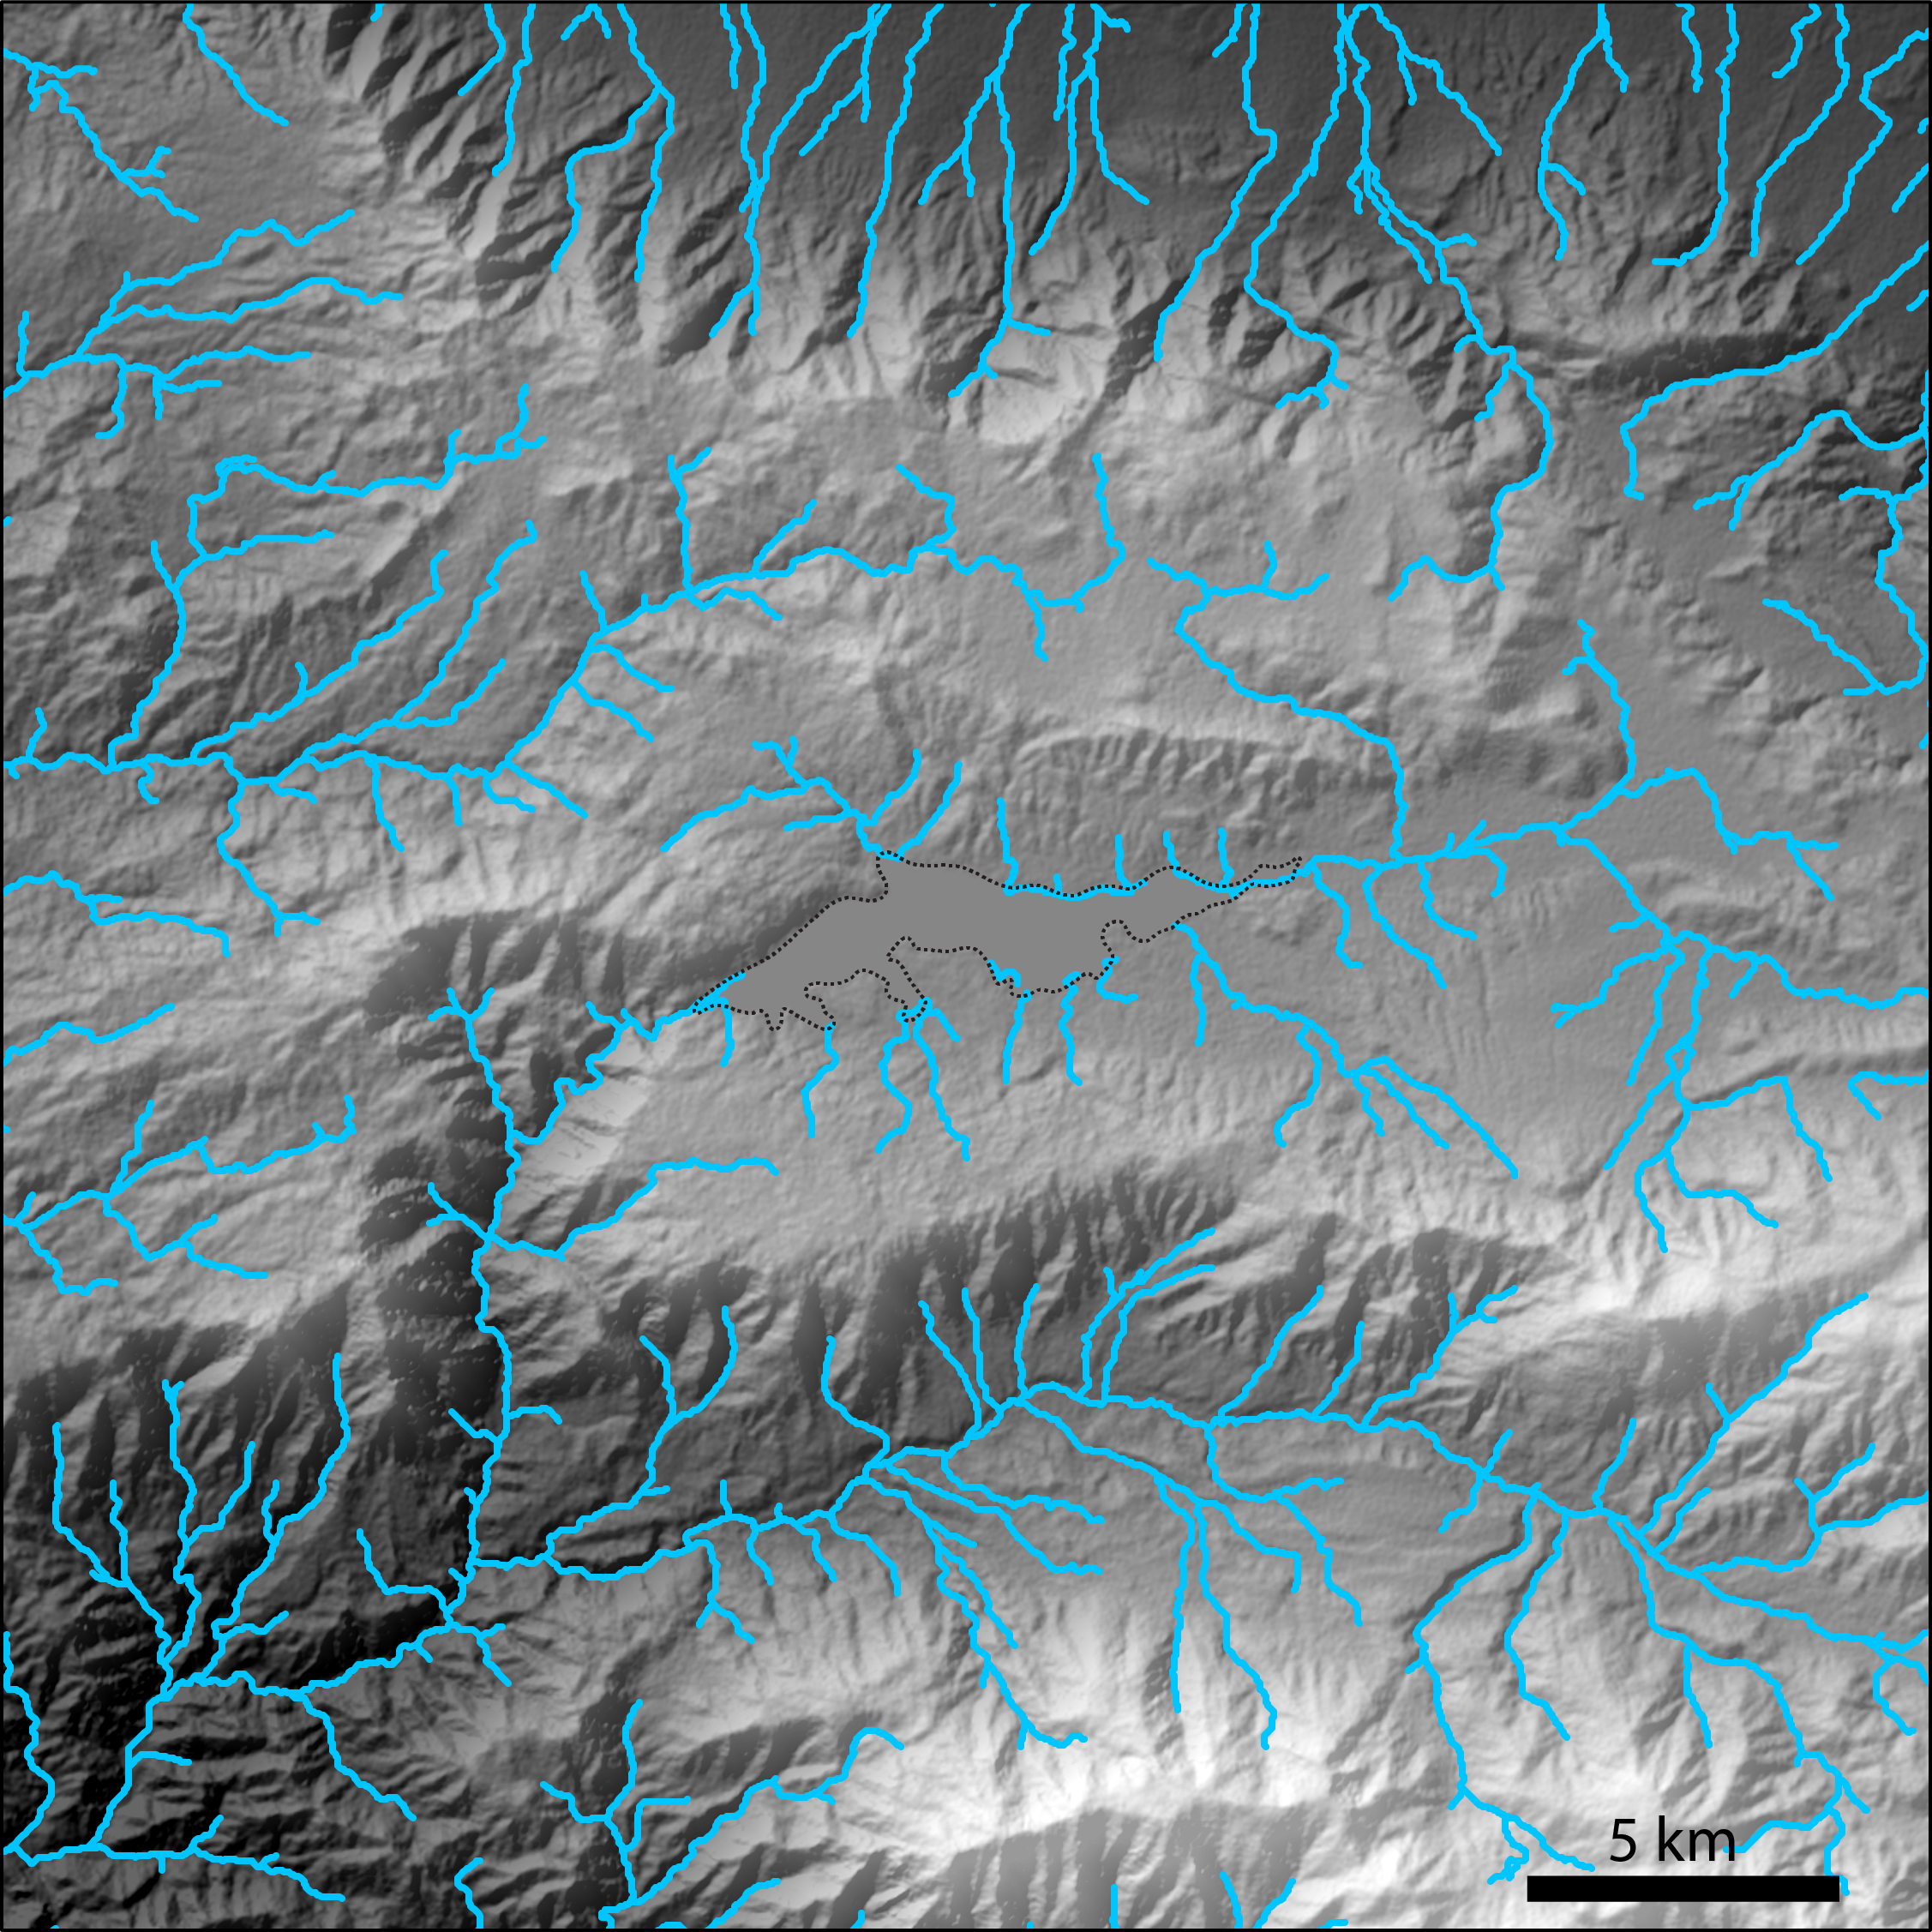
\includegraphics[width=.8\linewidth]{PNGs/BigBear1e6.png}
		\caption{Minimum flat area of 1e6}
		\label{fig:mfsub1}
	\end{subfigure}%
	\begin{subfigure}{.40\textwidth}
		\centering
		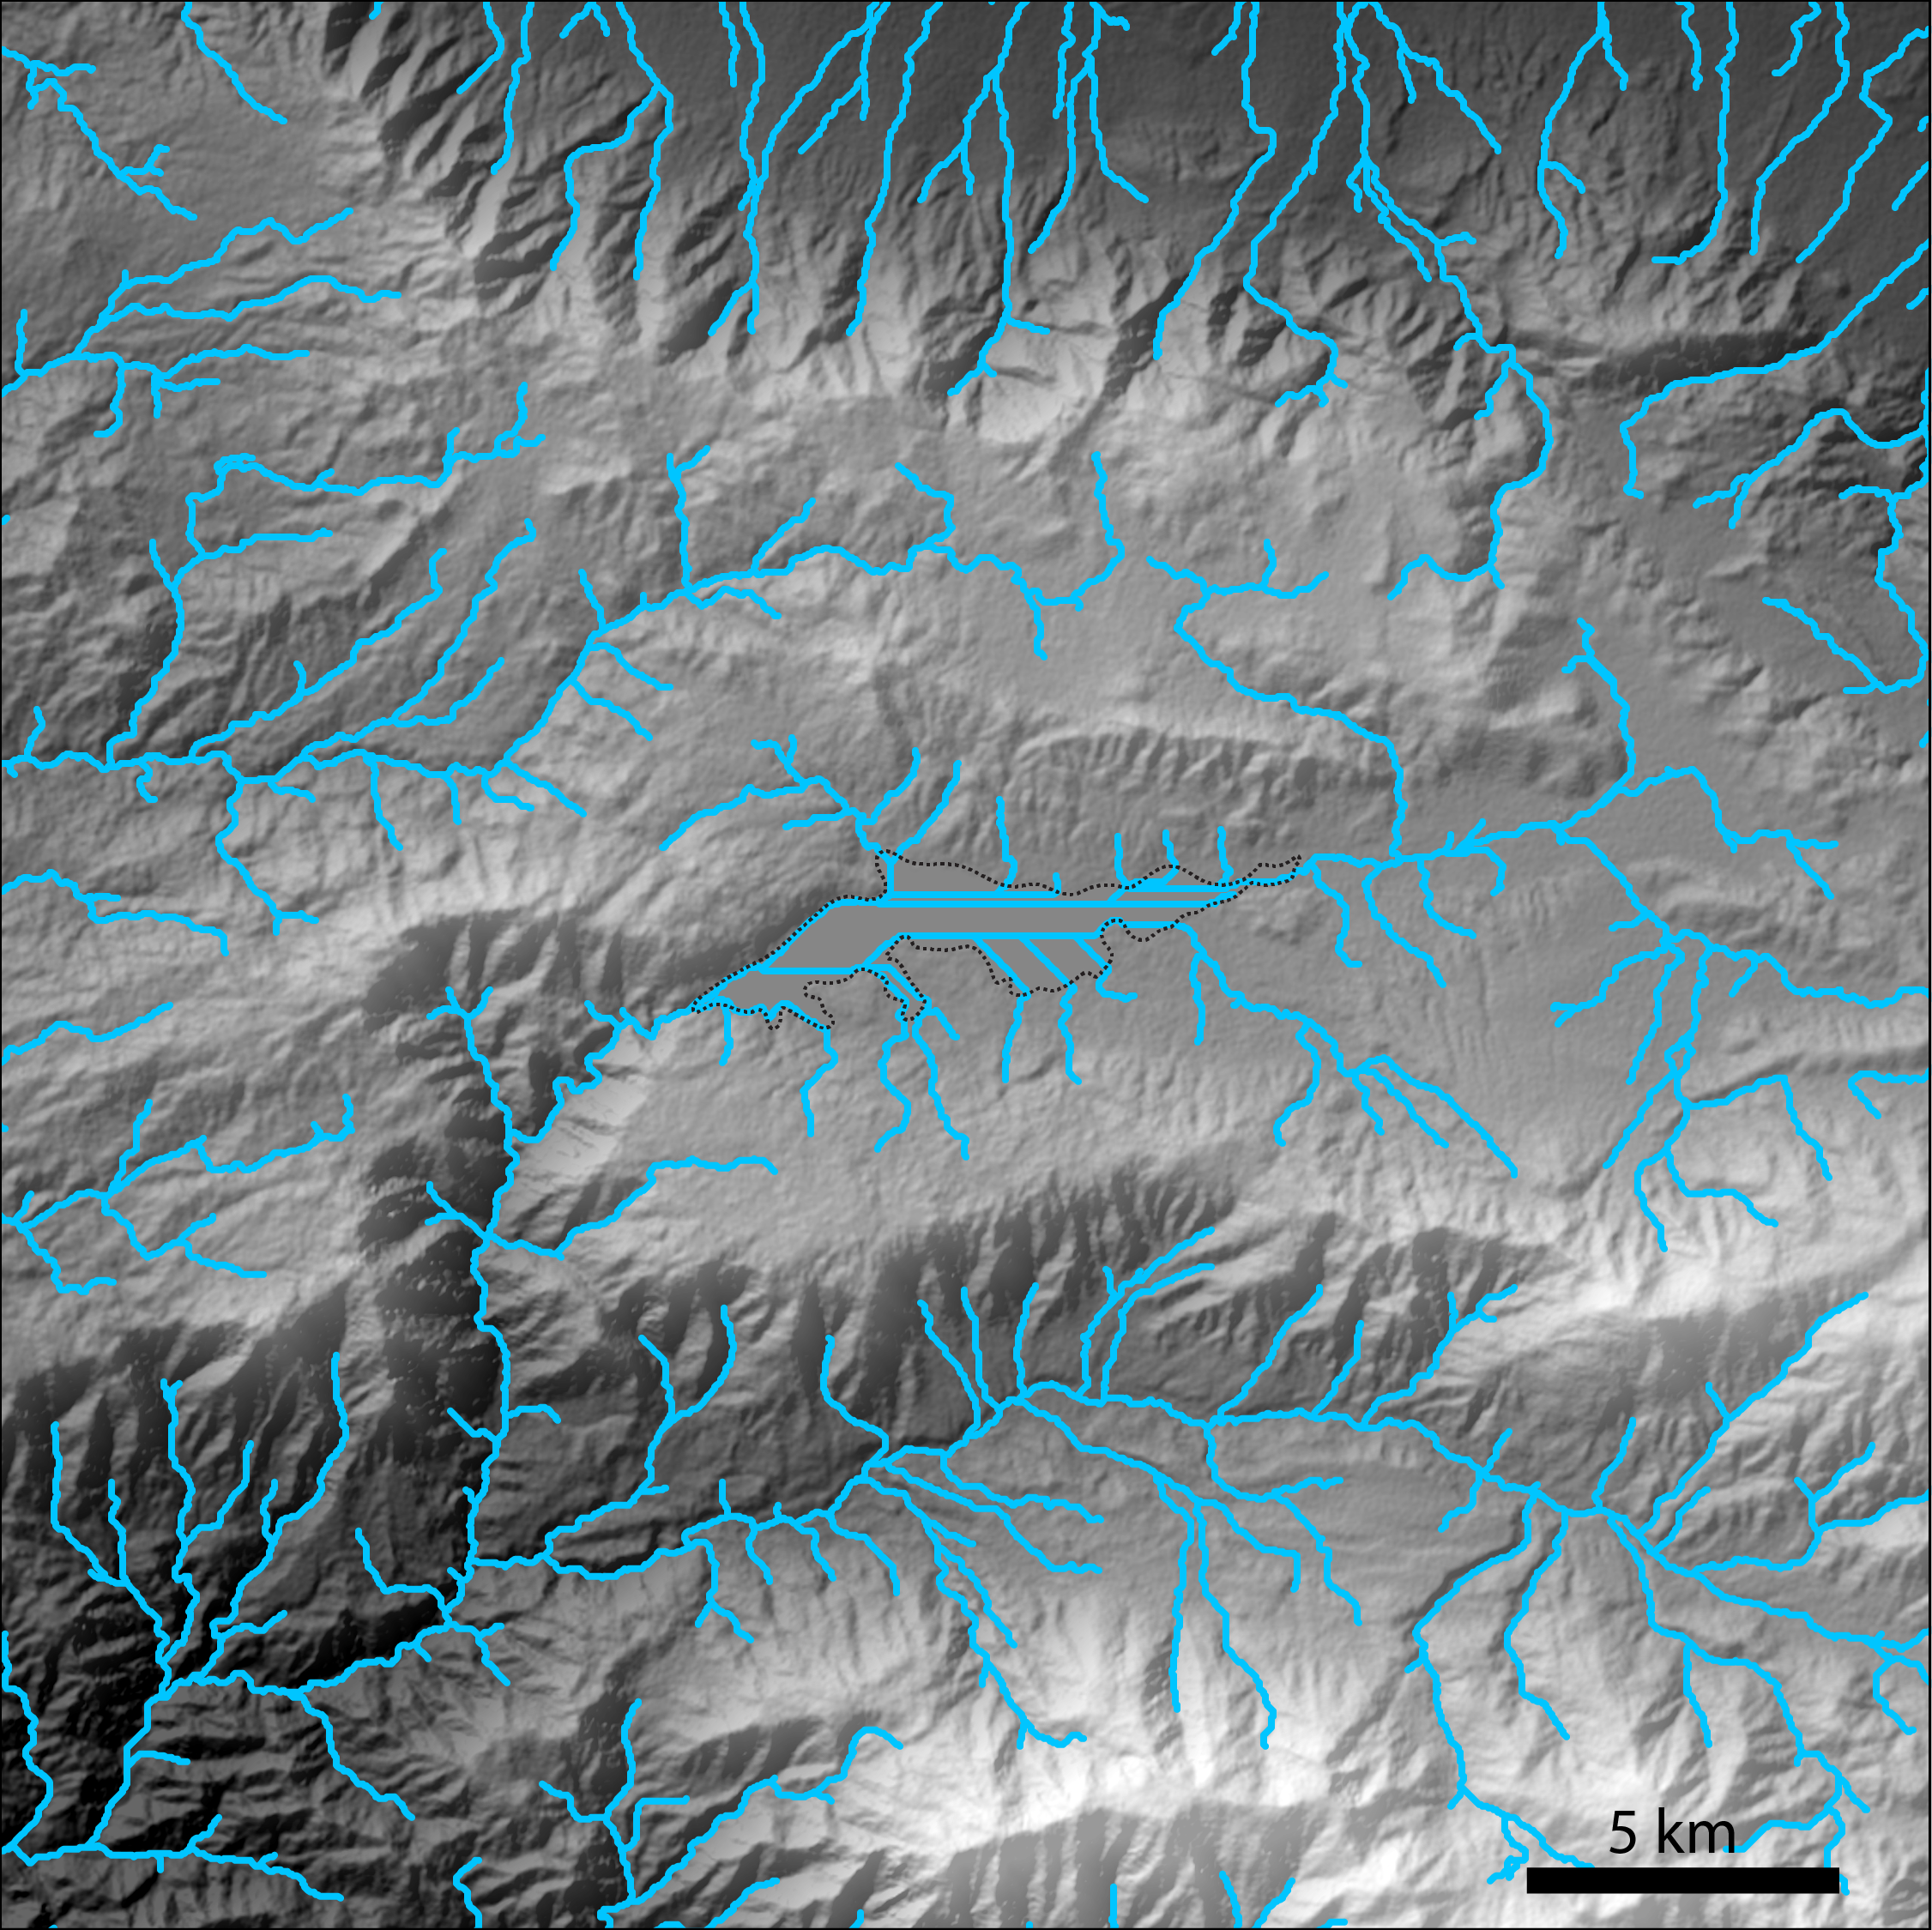
\includegraphics[width=.8\linewidth]{PNGs/BigBear1e7.png}
		\caption{Minimum flat area of 1e7}
		\label{fig:mfsub2}
	\end{subfigure}
	\caption{Difference in output of \nameref{sec:MakeStreams} depending on value used for \textit{min\_flat\_area} when auto removing flat areas in the area around Big Bear lake (outline of lake is shown in thin dotted black line) in the San Bernadino Mountains. When \textit{min\_flat\_area} is 1e6 (\ref{fig:mfsub1}), the lake is identified as a flat and removed, but when \textit{min\_flat\_area} is 1e7 (\ref{fig:mfsub2}) the lake is not identified as a flat and thus streams are routed through the lake.}
	\label{fig:min_flat}
\end{figure}

\paragraph{}\textit{MakeStreams} also has controls for resampling the input DEM. This can be useful (and is sometimes necessary), because after reprojecting georeferenced data in a GIS program, the cellsize of the DEM can end up as a number with a lot of decimal places. This can cause problems in some TopoToolbox and TAK functions because of different rounding behaviors and thus cause the codes to think that two datasets do not line up, even when they do. To avoid this, \textit{MakeStreams} will warn you if the provided DEM does not have a whole number cellsize and suggest that you use the resample option to fix this for later processing. 

\paragraph{}\textit{MakeStreams} also has an options to provide a precipitation dataset (with or without a comparable runoff ratio grid) to automatically produce a weighted flow accumulation raster:

\begin{lstlisting}[language=Matlab]
PRECIP=GRIDobj('/Users/aforte/GISdata/prism_precip.tif');
[DEM,FD,A,S]=MakeStreams('/Users/aforte/GISdata/SoCal_UTM_DEM.txt',1e6,'precip_grid',PRECIP);
\end{lstlisting}

\paragraph{}Finally, for large DEMs, the flow routing can take a long time. To speed this up, you can call upon the 'mex' files associated with the flow routing routines by setting the \textit{'mex'} parameter to true. This will only work if you have precompiled the appropriate mex files from TopoToolbox on your machine, see the TopoToolbox function \textit{'compilemexfiles.m'} for more information.

\subsection{\textit{ConditionDEM}}

\paragraph{}DEMs can be extremely noisy and thus can produce very jagged stream profiles. This is both visually unappealing, but more importantly is problematic for calculations that use stream gradient (e.g. normalized channel steepness). TopoToolbox includes a variety of different algorithms to condition or smooth DEMs, either as an entire grid or specifically along specified stream networks. The \textit{ConditionDEM} function is a wrapper around all of these different routines. We refer readers to the TopoToolbox documentation for detailed discussions of these smoothing routines, including \cite{Schwanghart2017} for consideration of the 'crs' algorithm. Some are very computationally intensive and require several parameters, so you are advised to spend some time 'playing' with the parameters and choices to see the outcome. \textit{ConditionDEM} produces example stream profiles comparing the unconditioned and conditioned result along with a map showing where elevations were changed to aid you in understanding what the chosen algorithm has done. 

\paragraph{}It is not strictly required to use the \textit{ConditionDEM} function. All TAK functions that need smoothed channel profiles have built in conditioning, using the \textit{mincosthydrocon} algorithm with an interpolation value of 0.1. If you want to use a different conditioning algorithm, you can use \textit{ConditionDEM} to produce a conditioned DEM that you can then supply as an optional input to TAK functions that need a conditioned DEM.

\subsection{\textit{RemoveFlats}}

\paragraph{}For topographic analysis, standard stream routing algorithms will usually route streams through lakes and playas, which in some circumstances is inappropriate and could produce misleading results, so it can be helpful to remove these from DEMs or set them to no data to restrict stream definition. Some of this can be accomplished with the simple controls built into \nameref{sec:MakeStreams}, but when these flat areas are not perfectly flat or occur at multiple elevations, they can be problematic to remove without manual clipping of DEMs. The \textit{RemoveFlats} function is an attempt to partially automate this process. It allows you to graphically identify areas (with a single click for each connected flat area) that you consider flats and the function will attempt to find contiguous areas. The function first fills all sinks in the DEM and then performs a morhpological erosion on the filled DEM with a 3x3 neighborhood. This means that any pixel will be set to the lowest elevation in a 3x3 neighborhood centered on that pixel. The eroded DEM is then morphologically dilated, with a neighborhood of between 3x3 to 9x9 depending on the users selection for the \textit{'strength'} parameter. This dilation sets pixels within the neighborhood to the maximum value. When the user then selects a location on the DEM, all pixels which are connected (using the dilated DEM) are identified as a flat and set to NaN.

\paragraph{}This function can sometimes be overly aggressive and remove areas of interest, so it is always best to inspect the results of the function before using it for subsequent processing (e.g. providing the filtered DEM produced here to \textit{MakeStreams} to regenerate a stream network) and compare it with the basic output of \textit{MakeStreams} to determine whether the results of \textit{RemoveFlats} are suitable for use.

\subsection{\textit{FindThreshold}} \label{sec:FindThresh}

\paragraph{}Stream definition is commonly controlled by a minimum threshold accumulation area, i.e. streams are defined as anywhere within a DEM where the upslope drainage area exceeds a threshold value. The \textit{FindThreshold} function is designed to aid you in choosing an appropriate minimum threshold area or, alternatively, manually setting this threshold area on a stream by stream basis. It requires that you run \textit{MakeStreams} initially, though the threshold area you use when running \nameref{sec:MakeStreams} is not critical (though this will dictate the initial drainage density and thus the number of channel heads with which to work). 

\paragraph{}\textit{FindThreshold} can be run in one of two ways. In the first way, when you provide a numeric input to the \textit{'num\_streams'} parameter, the function displays this user specified number of streams extracted all the way to the drainage divide and allows you to choose, on either a $\chi$-elevation or slope-area plot where you think the hillslope to channel transition might be. In this mode, the function will produce a new stream network based on the average of your minimum threshold area choices, and will also give you the population of minimum threshold areas and associated distances from the drainage divide to the channel head for the streams you choose. Alternatively, \textit{FindThreshold} if \textit{'num\_streams'} is set to \textit{'all'}, it runs in a mode where the function iterates through all channel heads in the provided stream network and uses the same picking protocol as above to manually set the minimum threshold area for each stream. In this mode each stream will have a variable minimum threshold area, but the total number of streams (i.e. channel heads) will still be dictated by the drainage density of the input stream network. Running \textit{FindThreshold} with \textit{'num\_streams'} set to \textit{'all'} on a large stream network may be very labor intensive, for example, the southern California dataset with an initial threshold area of 1e6 m\textsuperscript{2} has $>$ 120,000 channel heads so if you were to in \textit{'all'} mode, you would have to manually identify the hillslope-channel transition on ALL of those channel heads.

%%%%%%%%
\section{Stream Selection and Projection}

\paragraph{}The three functions for stream selection and projection have some overlap with similar functions in TopoToolbox, but are slightly different in implementation or style of outputs. Exploring both to see which set better fits your needs is advisable.

\subsection{\textit{SegmentPicker}} \label{sec:SegPick}
\paragraph{}\textit{SegmentPicker} is a function designed to select portions of larger stream networks. In terms of stream selection, the function has two primary modes, either 'down', i.e. you select individual streams based on a channel head location, or 'up', i.e. you select portions of networks above a given pour point. If selecting on the basis of channel head location, the function will interpret your selection to be the channel head that is the minimum euclidean distance between your selection and the actual channel heads. Channel selection can be done interactively within Matlab or by providing coordinates of channel heads or pour points as an array or a point shapefile. \textit{SegmentPicker} shares some similarity to the TopoToolbox function \textit{flowpathapp} or functionality available in \textit{topoapp}.

\subsection{\textit{SegmentPlotter}}
\paragraph{}\textit{SegmentPlotter} takes the output of \nameref{sec:SegPick} and plots each selected stream individually. The stream network is plotted as $\chi$-elevation, longitudinal profile, and slope-area plots. With the logical \textit{'separate'} flag, you can produce individual figures for each segment. Alternatively, you can provide a list of identifying numbers (i.e. the ID number in the third column of the \nameref{sec:SegPick} output) to the \textit{'subset'} parameter to only plot specific segments. You can also initiate and control labeling of stream segments with the \textit{'label'} and \textit{'names'} parameters.

\subsection{\textit{SegmentProjector}}

\paragraph{}\textit{SegmentProjector} allows you to interactively select a portion of a stream to project along the length of the entire stream (i.e. from the mouth to the channel head of the provided stream). This can be useful for a variety of questions, e.g. estimating the amount of uplift of a low relief portion of a landscape (Figure \ref{fig:proj1}) or identifying portions of a stream profile that may be tectonically deformed or otherwise disturbed (Figure \ref{fig:proj2}). In detail, the function clips out the portion of the stream you select and performs a least squares linear fit on the $\chi$-elevation relationship along with a 95\% confidence interval on this fit. 

\begin{figure}[H]
	\centering
	\begin{subfigure}{.5\textwidth}
		\centering
		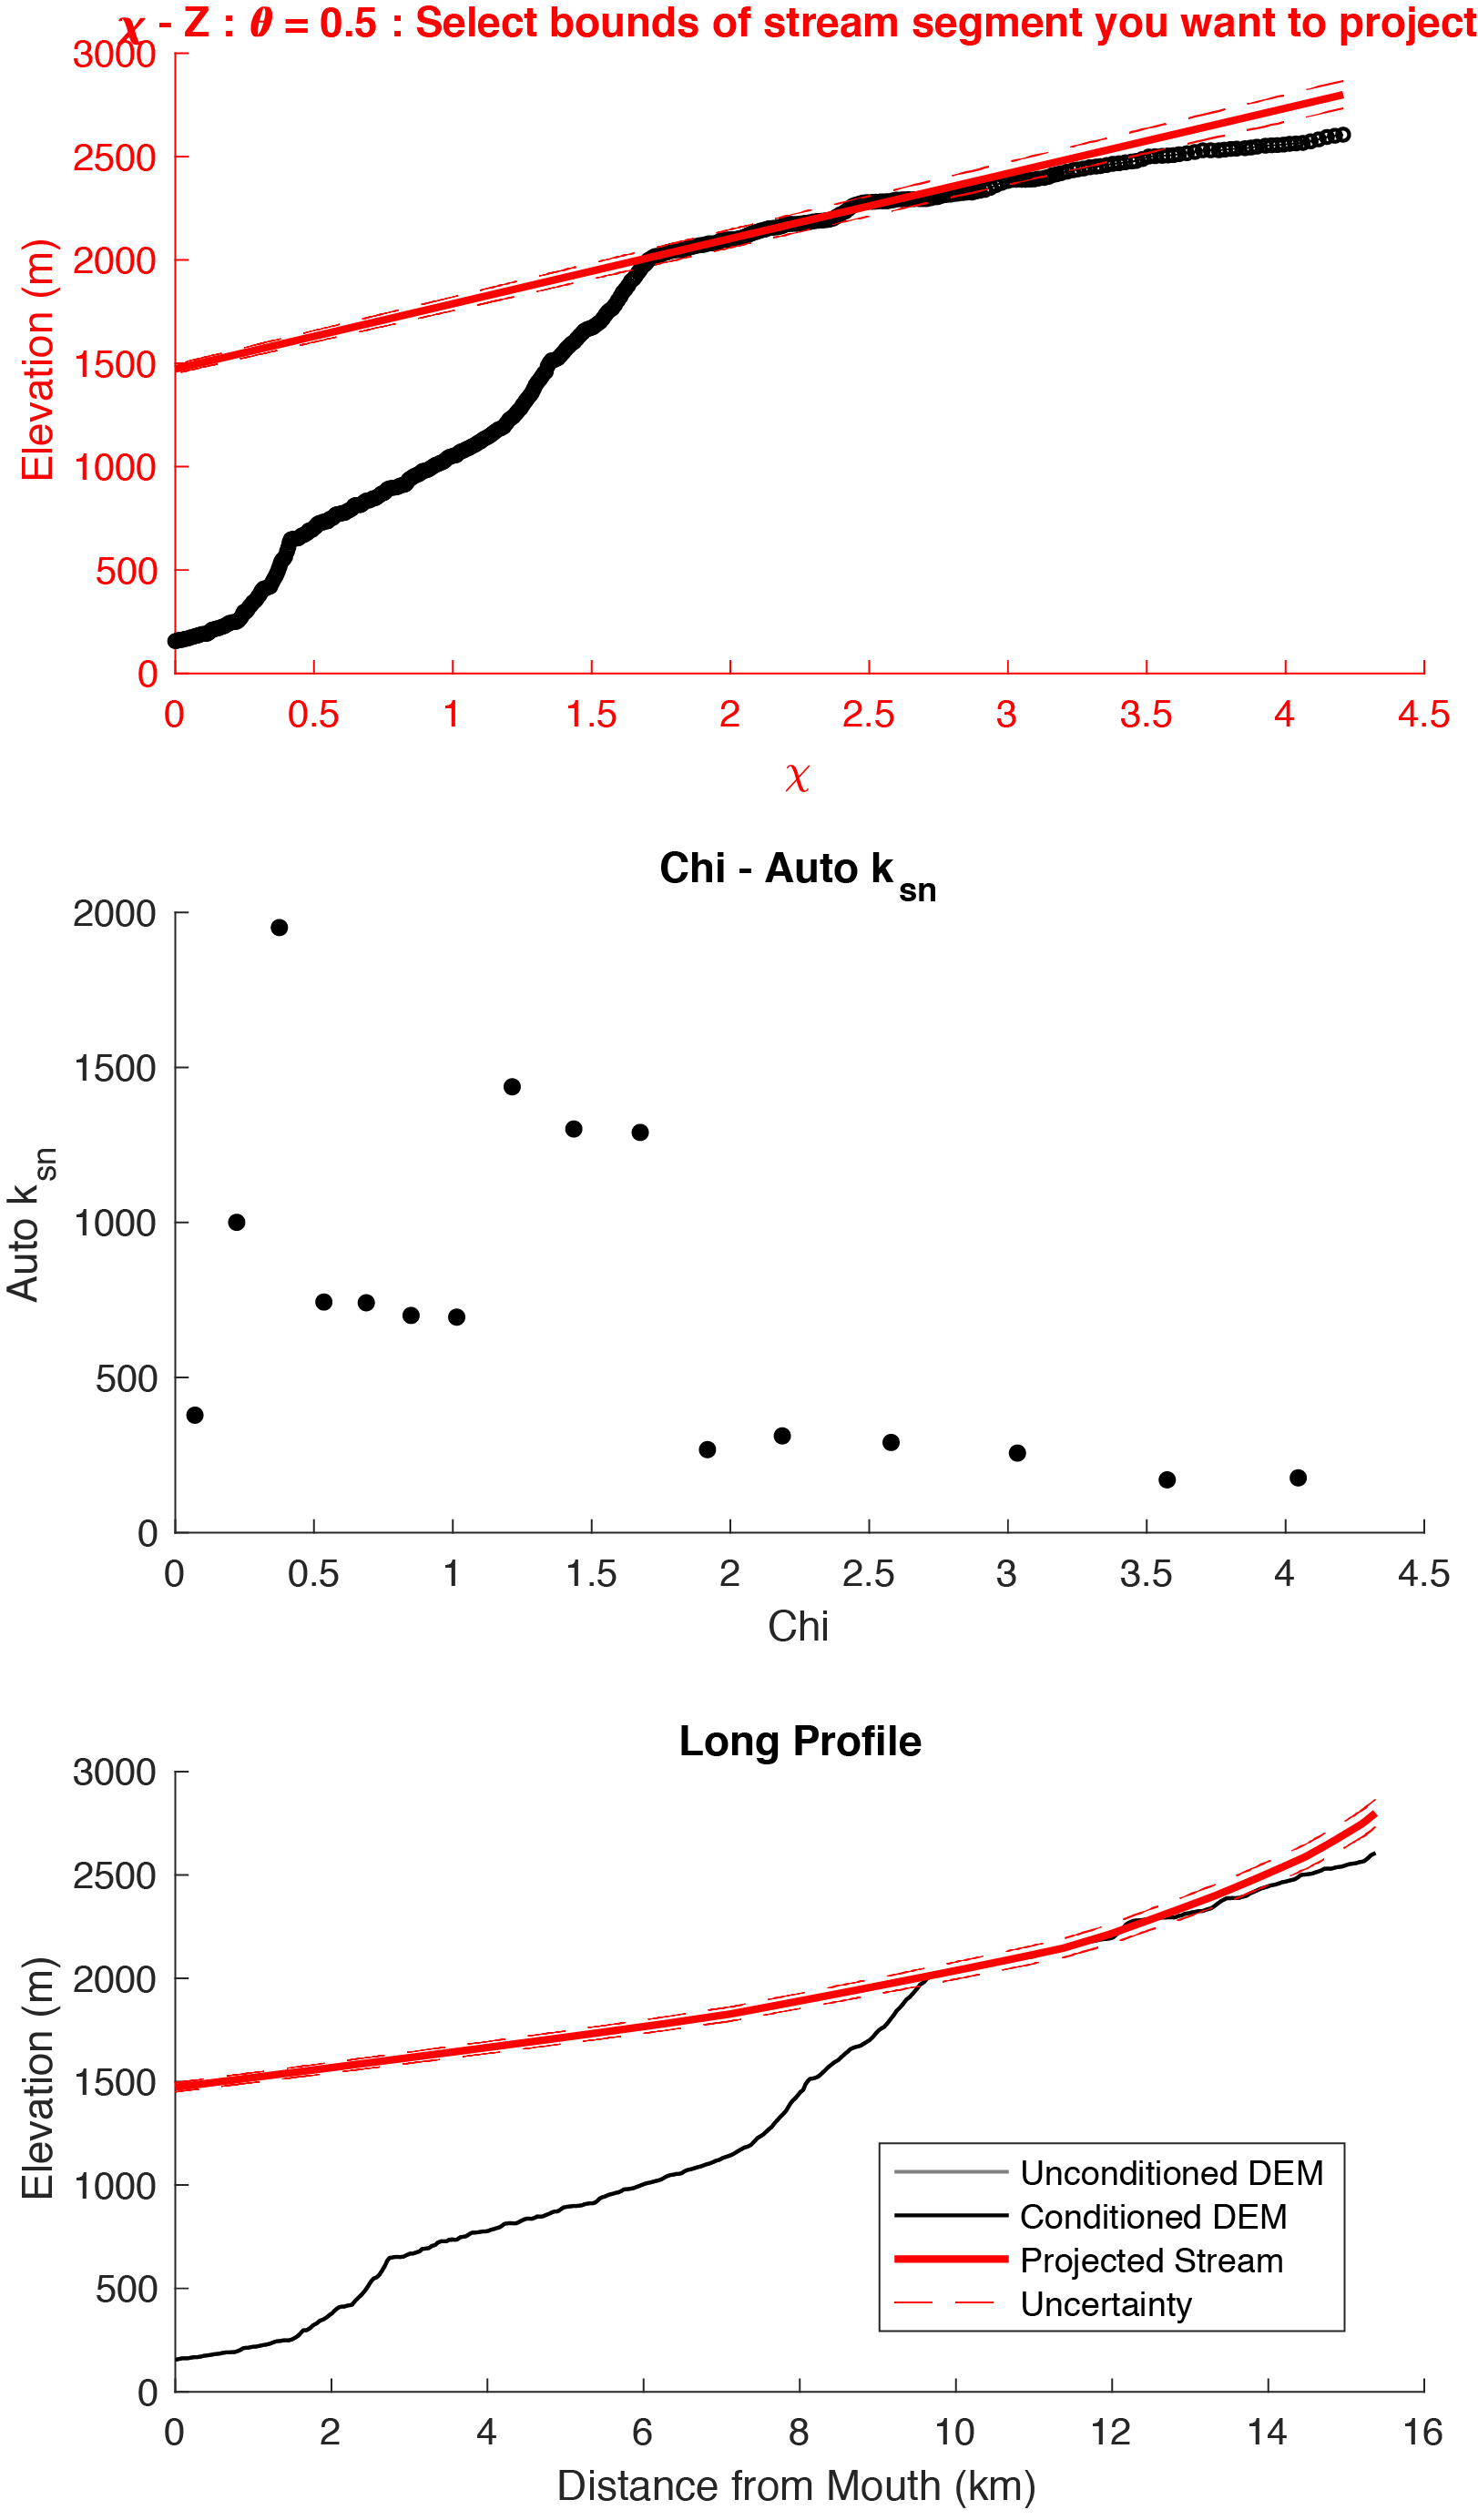
\includegraphics[width=.8\linewidth]{PNGs/B402_ProjectedProfile_1.png}
		\caption{Projected stream}
		\label{fig:p1sub1}
	\end{subfigure}%
	\begin{subfigure}{.5\textwidth}
		\centering
		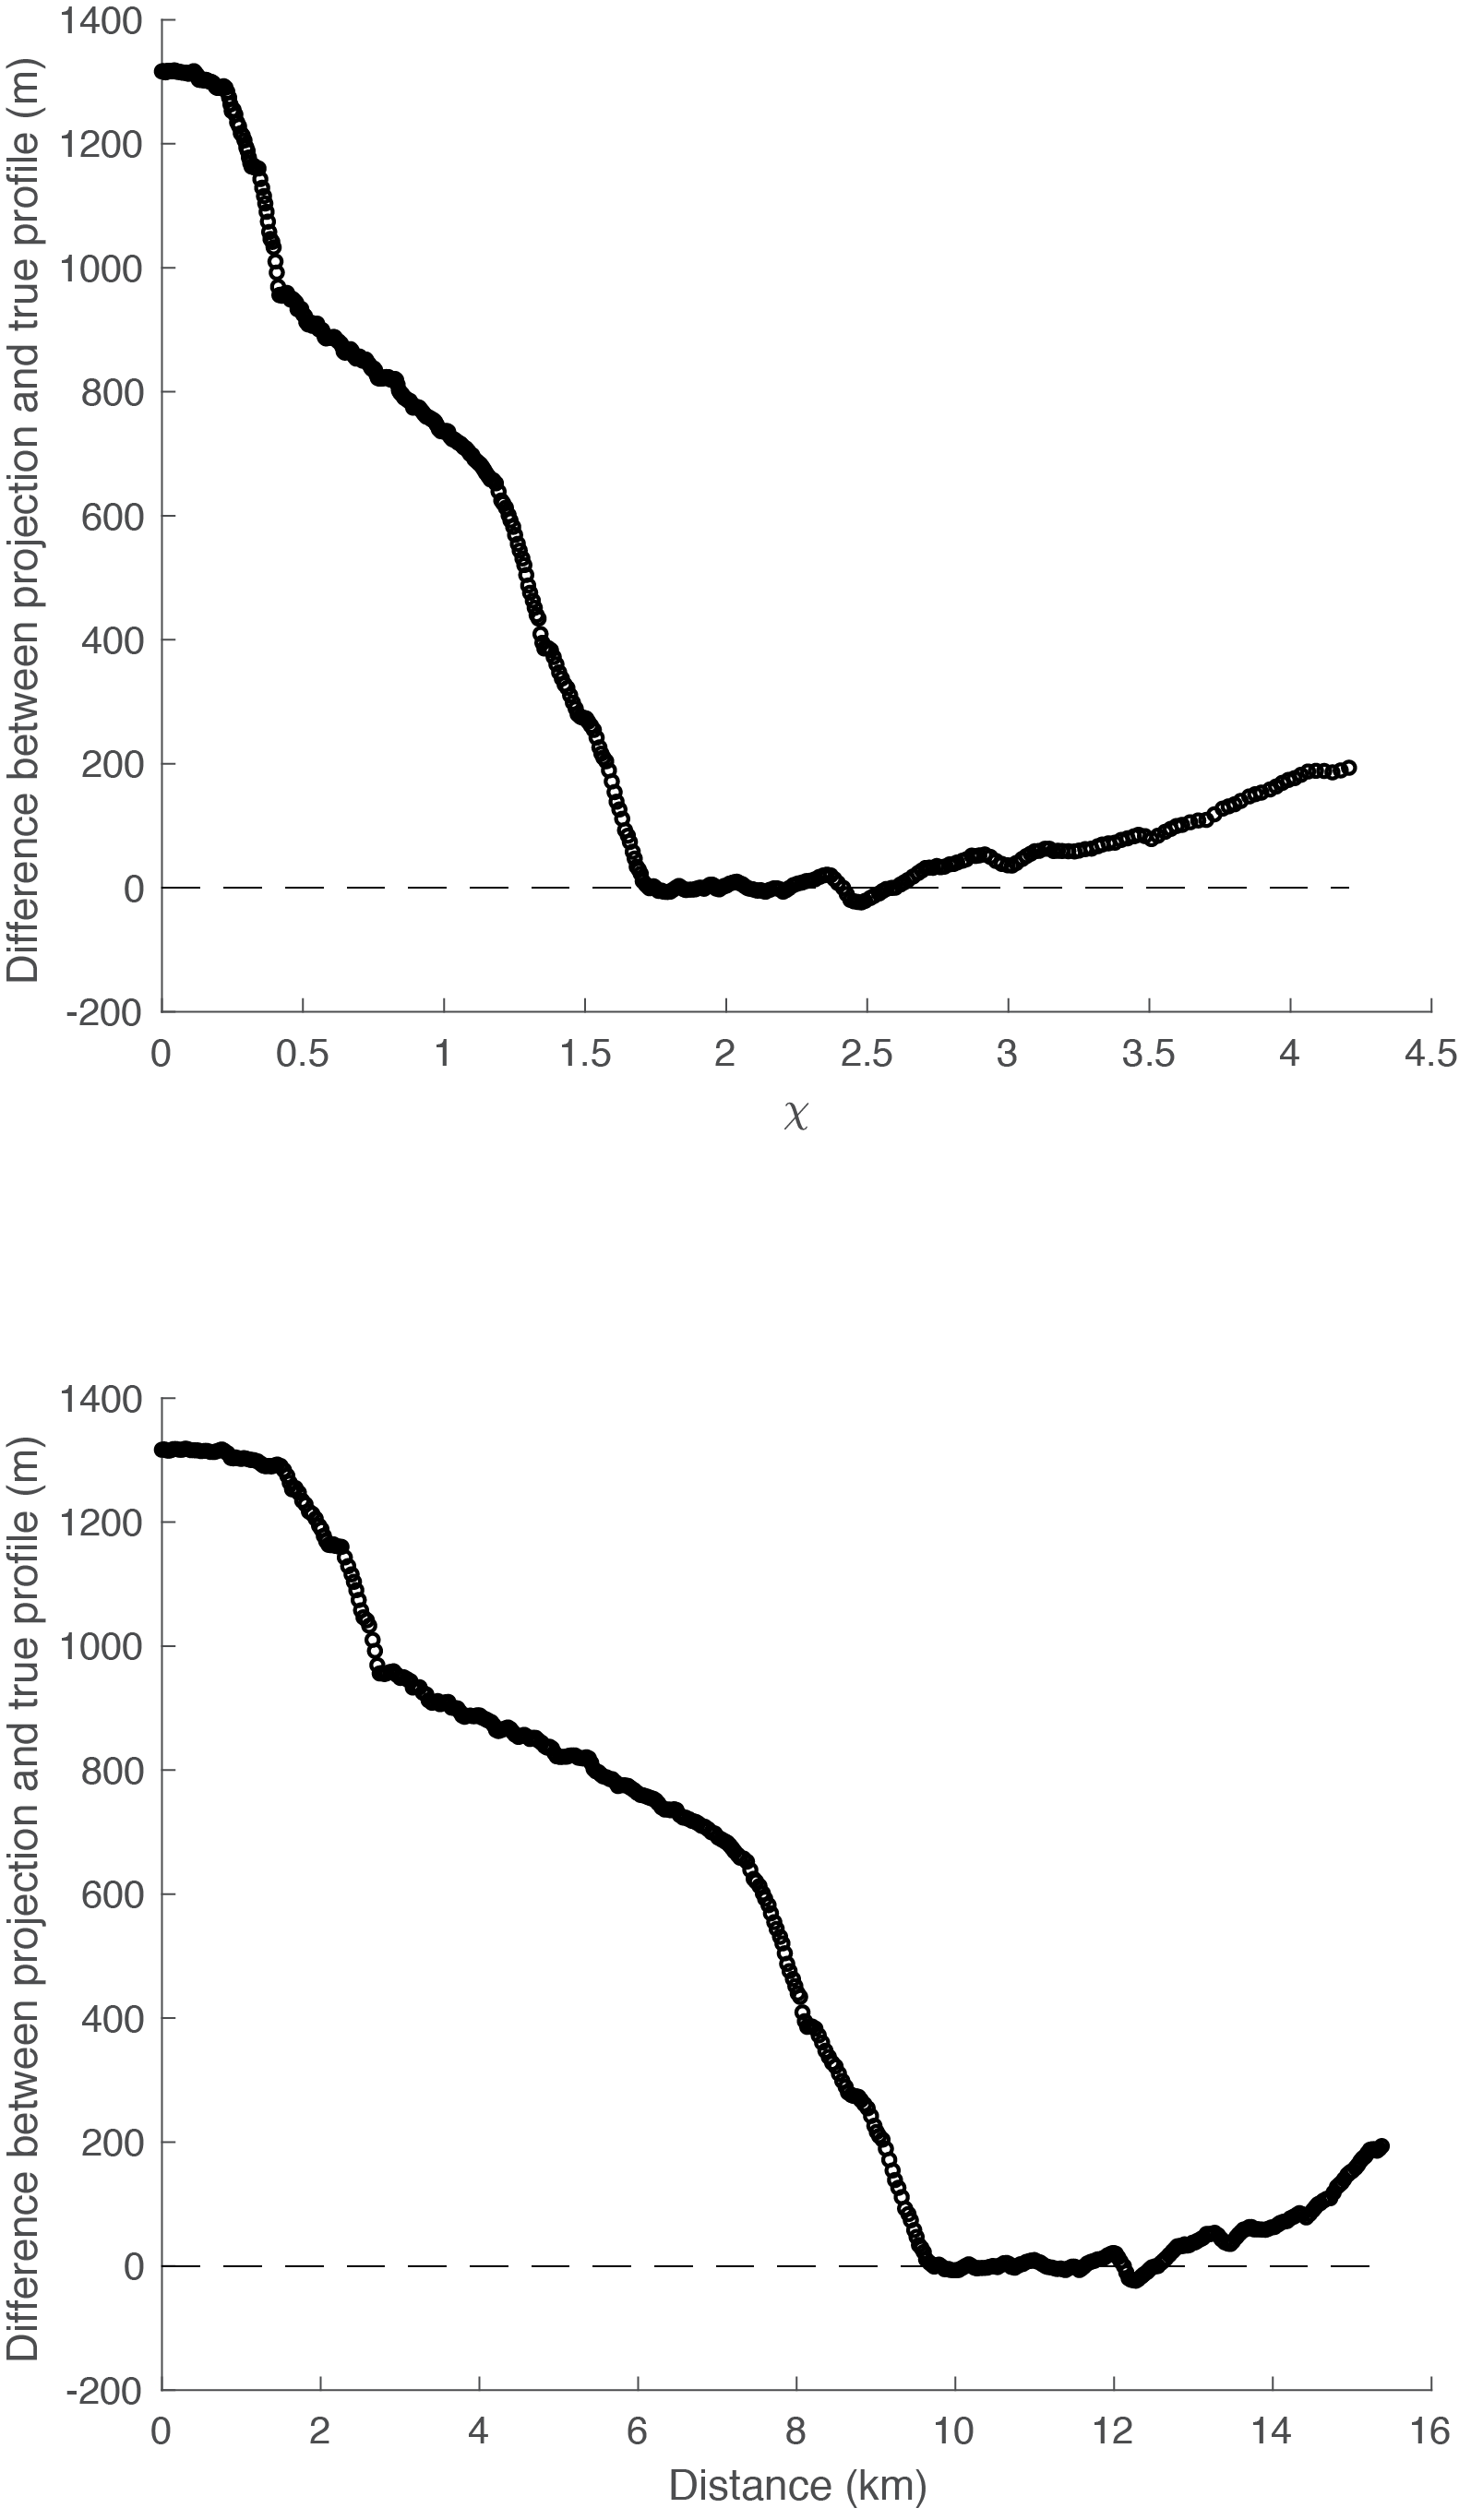
\includegraphics[width=.8\linewidth]{PNGs/B402_ProjResidual_1.png}
		\caption{Residual on projected stream}
		\label{fig:p1sub2}
	\end{subfigure}
	\caption{Example of \textit{SegmentProjector} outputs for a stream within Basin 402 (northeastern San Jacinto Mountains) with a low relief upper portion.}
	\label{fig:proj1}
\end{figure}

\begin{figure}[H]
	\centering
	\begin{subfigure}{.5\textwidth}
		\centering
		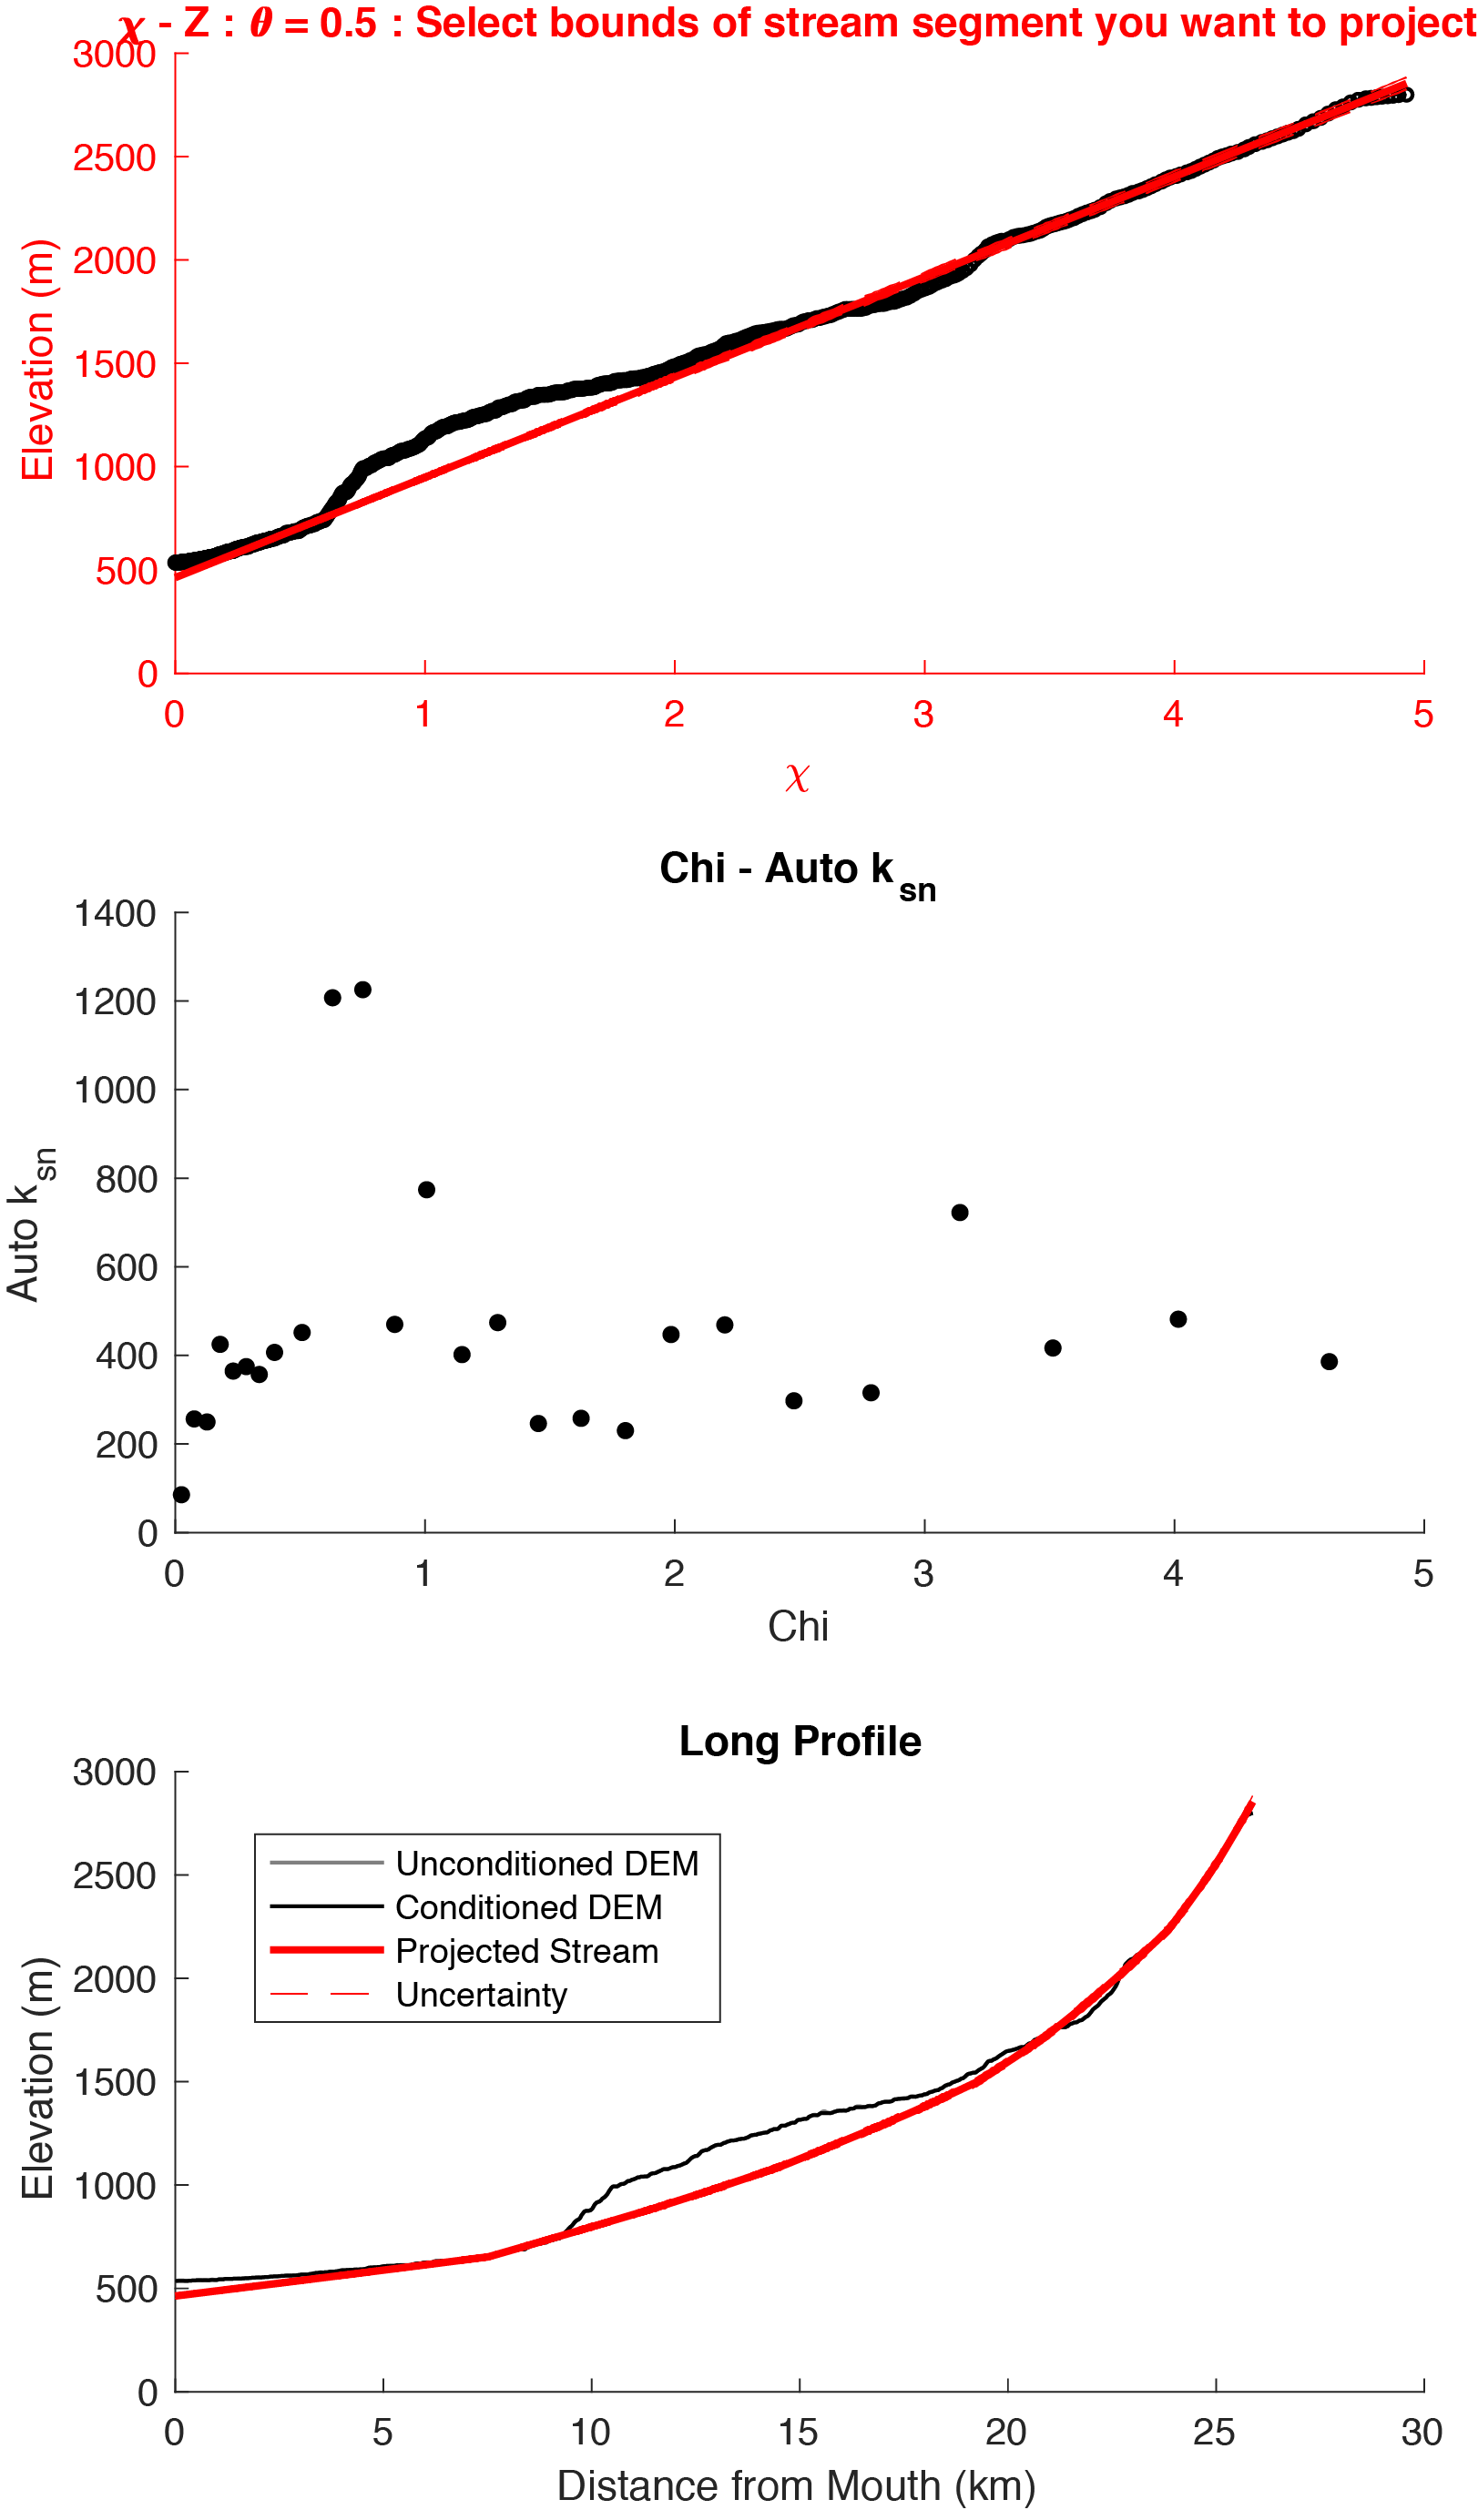
\includegraphics[width=.8\linewidth]{PNGs/B313_ProjectedProfile_1.png}
		\caption{Projected stream}
		\label{fig:p2sub1}
	\end{subfigure}%
	\begin{subfigure}{.5\textwidth}
		\centering
		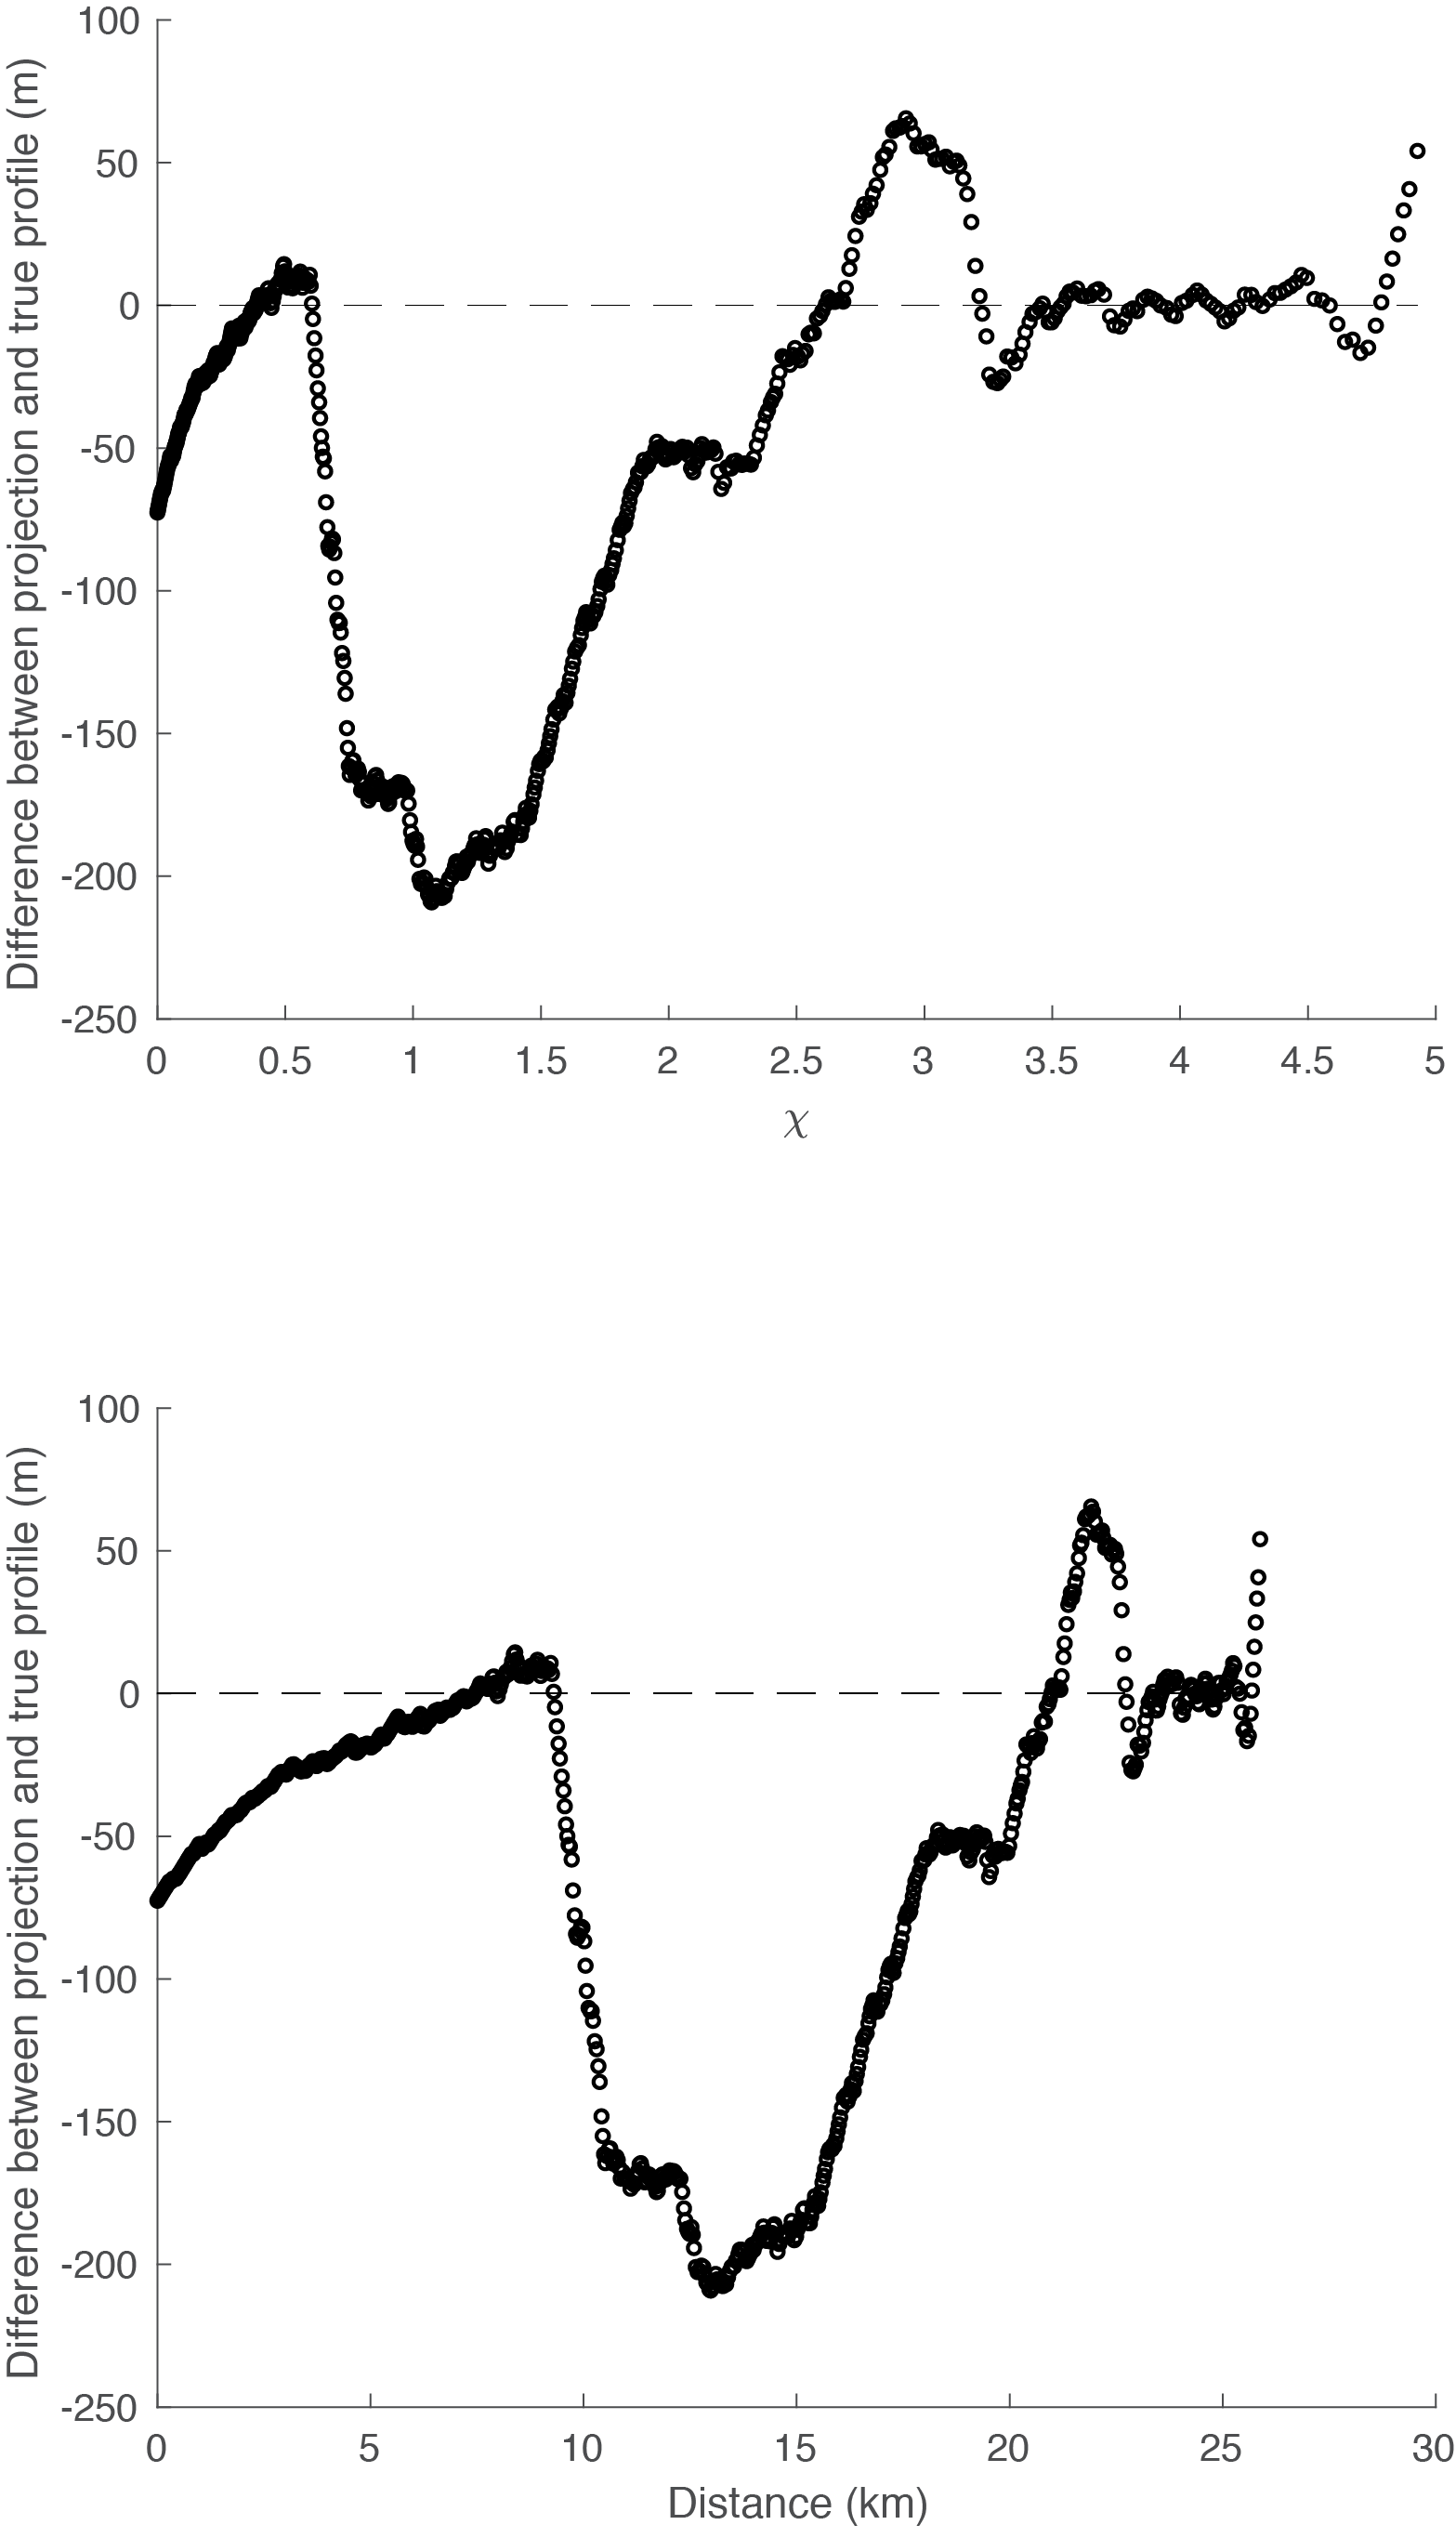
\includegraphics[width=.8\linewidth]{PNGs/B313_ProjResidual_1.png}
		\caption{Residual on projected stream}
		\label{fig:p2sub2}
	\end{subfigure}
	\caption{Example of \textit{SegmentProjector} outputs for a stream within Basin 313 (northwestern San Jacinto Mountains) with possible localized deformation or landslide deposit within the profile.}
	\label{fig:proj2}
\end{figure}

\paragraph{}\textit{SegmentProjector} will iterate through all channel heads within a provided stream network, so it is suggested that you use \nameref{sec:SegPick} or some other means of selecting streams of interest before running \textit{SegmentProjector}. Note that if you are using the output of \textit{SegmentPicker}, you will need to load the \textit{PickedSegments\_*.mat} file and provide the \textit{STREAMobj} \textit{Sc} stored within this file as the required \textit{STREAMobj} input to \textit{SegmentProjector}. \textit{SegmentProjector} is similar to the TopoToolbox \textit{streamproj} function.

\subsection{\textit{ProjectedIncision}}
\paragraph{}Temporary

%%%%%%%%
\section{Channel Steepness and $\chi$ Maps}

\subsection{\textit{KsnChiBatch}} \label{sec:KsnBatch}
\paragraph{}\textit{KsnChiBatch} is designed to be similar to the original 'batch' mode in Profiler51 for creating normalized channel steepness (\textit{k\textsubscript{sn}}) maps, but has many more options. \textit{KsnChiBatch} can be used to produce stream networks with values of \textit{k\textsubscript{sn}}  or $\chi$ or continuous grids of either \textit{k\textsubscript{sn}} or $\chi$. There are options to produce outputs as either shapefiles or ascii grids for use in a GIS program or matlab outputs for display (e.g. using \nameref{sec:plotksn}) or for analysis. There are also options to remove incomplete portions of stream networks (which can be problematic for both $\chi$ and \textit{k\textsubscript{sn}} calculations) and control outlet elevation (which can be important for correctly interpreting $\chi$ anomalies). The methodology employed for dealing with $\chi$ in \textit{KsnChiBatch} is identical to that as in the companion \href{https://github.com/amforte/DivideTools}{DivideTools GitHub repository}, the details of which are described in \cite{Forte2018a} \href{https://www.sciencedirect.com/science/article/pii/S0012821X18302292}{[Link to Journal Site]} .

\paragraph{}The outputs of the \textit{KsnChiBatch} function differ depending on the type of map being calculated. If the required \textit{'product'} input is set to \textit{'ksn'}, then the function will save a polyline shapefile, but if the \textit{'product'} is \textit{'chi'}, \textit{'chigrid'}, or \textit{'ksngrid'} the function will save an ascii grid. $\chi$ maps are output as grids to avoid averaging of chi values along a stream network during the production of a shapefile. If you wish to create a shapefile of a $\chi$ map, you can use a GIS program to create a shapefile from the ascii grid (e.g. in ArcGIS, convert the ascii to a raster and then use the raster to polyline function).

\paragraph{}You can also specify that you want the function to produce outputs to the workspace with the optional \textit{'output'} parameter. The number of outputs will again vary with the product:

\begin{lstlisting}[language=Matlab]
% When 'ksn' is the 'product', two outputs will be produced, a GRIDobj with averaged ksn values stored in nodes along the stream network  (KSN_STREAM_GRID) and a geographic information structure of ksn values (ksn_ms)
[KSN_STREAM_GRID,ksn_ms]=KsnChiBatch(DEM,FD,A,S,'ksn');
% When 'ksngrid' is the product, a GRIDobj of interpolated ksn values will be produced
[KSN_GRID]=KsnChiBatch(DEM,FD,A,S,'ksngrid');
% When 'chimap' is the product, a GRIDobj with chi values stored in nodes along the stream network will be produced
[CHI_MAP]=KsnChiBatch(DEM,FD,A,S,'chimap');
% When 'chigrid' is the product, a GRIDobj with chi values in all nodes not excluded by outlet conditions will be produced
[CHI_GRID]=KsnChiBatch(DEM,FD,A,S,'chigrid');
% When 'chi' is the product, the chi map output will come first
[CHI_MAP,CHI_GRID]=KsnChiBatch(DEM,FD,A,S,'chi');
% When 'all' is the product, all of the previous outputs will be produced in the following order
[KSN_STREAM_GRID,ksn_ms,KSN_GRID,CHI_MAP,CHI_GRID]=KsnChiBatch(DEM,FD,A,S,'all');
\end{lstlisting}

\paragraph{}Values of \textit{k\textsubscript{sn}} can be calculated in three primary ways. The default \textit{'ksn\_method'} (and the same method used in the original Profiler51 or the TopoToolbox \textit{ksn} function) is denoted \textit{'quick'} and calculates \textit{k\textsubscript{sn}} across the entire stream network simultaneously by solving the equation, 

\begin{equation}
 S=k_{sn}*A^{-\theta}
\end{equation}

\noindent where $S$ is the gradient, $A$ is the drainage area, and $\theta$ is a reference concavity. This result will typically be extremely noisy because of small variations in gradient, so \textit{k\textsubscript{sn}} values are usually averaged over some length, depending on the resolution of the data, \citep[e.g.,][]{Wobus2006}. This \textit{'smooth\_distance'} is a user controlled parameter in \textit{KsnChiBatch}. 

\paragraph{}Because of the way the averaging is done over a given smoothing distance by the underlying TopoToolbox \textit{STREAMobj2mapstruct} function, sometimes portions of trunk streams can end up with anomalously high \textit{k\textsubscript{sn}} values as their values are influenced by smaller, steeper side tributaries. To partially control for this, we include an additional method of \textit{k\textsubscript{sn}} calculation where averaged \textit{k\textsubscript{sn}} values for trunk streams are calculated separately. This option can be used by setting \textit{'ksn\_method'} to \textit{'trunk'}. The determination of whether a stream is a trunk stream or not is based on stream order, which is controllable with the optional \textit{'min\_order'} parameter. By default, the \textit{'min\_order'} is set to 4, meaning that any stream of order 4 or greater is considered a trunk stream.

\paragraph{}Both the default \textit{'quick'} and \textit{'trunk'} methods described above are rapid to calculate, but can sometimes smear out true abrupt changes in \textit{k\textsubscript{sn}} at confluences. For this reason, by setting \textit{'ksn\_method'} to \textit{'trib'}, \textit{k\textsubscript{sn}} can also be calculated with \textit{KsnChiBatch} where network segments (i.e. stream segments between confluences) are selected, divided into sub-segments determined by the \textit{'smooth\_distance'}, and then the average \textit{k\textsubscript{sn}} of each sub-segment is calculated by finding the best fit slope on the $\chi$-elevation relationship for this sub-segment (\textit{k\textsubscript{sn}} is equivalent to the slope of the $\chi$-elevation relationship when the reference drainage area is set to 1). The \textit{'quick'} and \textit{'trib'} methods do produce different \textit{k\textsubscript{sn}} patterns, though while subtle, do show some systematic behavior (Figure \ref{fig:BatchComp}).

\begin{figure}[H]
	\includegraphics[width=16.5cm]{PNGs/Batch_Comparison.png}
	\caption{Comparison of the regular 'quick' method vs the 'tributary' method of calculating \textit{k\textsubscript{sn}} using \textit{KsnChiBatch}.}
	\label{fig:BatchComp}
\end{figure}

\paragraph{}While we have not conducted a full study of the differences of the basic \textit{'quick'} vs \textit{'trib'} methods, the southern California example suggests that generally the regular \textit{'quick'} method of \textit{k\textsubscript{sn}} calculation may be slightly biased towards higher \textit{k\textsubscript{sn}} values, though 90\% of \textit{k\textsubscript{sn}} values of the two methods are within $\pm$50 of each other (this is with a reference concavity of 0.50, so absolute magnitudes of \textit{k\textsubscript{sn}} and thus magnitudes of deviations between these two methods will scale with choice of reference concavity). The \textit{k\textsubscript{sn}} values from the regular method are generally systematically larger than the tributary method values in low relief areas, where as generally \textit{k\textsubscript{sn}} values from the tributary method tend to be higher than regular values in higher relief portions of the landscape (Figure \ref{fig:BatchComp}). 

\paragraph{}The geographic information structure (and shapefile) produced from both methods for each segment (controlled by the \textit{'smooth\_distance'}) will have fields containing values for \textit{k\textsubscript{sn}} (\textit{'ksn'}), mean drainage area (\textit{'uparea'}), mean gradient (\textit{'gradient'}), and the difference between the conditioned stream elevation and non-conditioned stream elevation (\textit{'cut\_fill'}) to inform the user whether an anomalous \textit{k\textsubscript{sn}} value may because of an overly aggressive conditioning scheme. If the \textit{'trib'} method is used, the geographic information structure and shapefile will include an extra field, \textit{'chi\_r2'}, which is the R\textsuperscript{2} value on the $\chi$-elevation fit and can be interpreted as a measure of the linearity of each sub-segment. 

\paragraph{}If the \textit{'product'} is set to to \textit{'ksngrid'}, the continuous map of k\textsubscript{sn} is made via spatial averaging within a moving circular window of the individual k\textsubscript{sn} values along streams. The radius of this window by default is set to 5000 meters, but can be controlled via the \textit{'radius'} function. Note that the production of this continuous map of k\textsubscript{sn} can be time consuming. This output is suitable for use with the \nameref{sec:EroGrid} function.

\subsection{\textit{KsnProfiler}} \label{sec:KsnProfiler}

\paragraph{}For detailed analysis of streams, it is often necessary to manually select knickpoint bounded steam segments for which you wish to calculate average \textit{k\textsubscript{sn}} values. This was the primary purpose of the original Profiler51 code and we have produced the \textit{KsnProfiler} function to replicate and improve upon the original Profiler51 methodology. In detail, \textit{KsnProfiler} calculates \textit{k\textsubscript{sn}} of user selected segments by finding the best fit linear slope of the $\chi$-elevation relationship for the segment in question. It should be noted that 1) calculation of \textit{k\textsubscript{sn}} via this method will produce identical results to finding the intercept of a fit in slope-area space (providing that the reference area in the $\chi$ calculation is set to 1, as it is in \textit{KsnProfiler}) so there is no need to distinguish between \textit{k\textsubscript{sn}} values calculated by a $\chi$-elevation slope or a slope-area intercept and 2) though the publication associated with the original Profiler51 codes discussed \textit{k\textsubscript{sn}} calculation in terms of slope intercepts \citep{Wobus2006}, internally, the code used the slope of a linear fit on a $\chi$-elevation relationship to calculate \textit{k\textsubscript{sn}}. \textit{KsnProfiler} has a large number of optional inputs, so you should familiarize yourself with all of the ways in which it can be run by reading through the header of the function. We highlight some of the main options in the following sections.

\subsubsection{Stream Selection}
\paragraph{}There are four different ways in which you can define which streams you would like to fit. The default is an interactive channel selection method where you choose streams (from all of the streams in the provided \textit{STREAMobj}) manually by clicking near a channel head of interest. In this case, the call of \textit{KsnProfiler} is relatively simple:

\begin{lstlisting}[language=Matlab]
[~,~,~,~]=KsnProfiler(DEM,FD,A,S);
\end{lstlisting}

\noindent
 While this can be nice especially as it will update the map with \textit{k\textsubscript{sn}} values as you continue to pick and fit streams, it can be unstable or slow if you are trying to analyze a very large area (though you can use the \textit{'plot\_type'} parameter to switch to a map plot that is more optimized for larger datasets). The three other selection methods do not involve a map of streams, so is generally more stable for large datasets. The other options are called like:
 
 \begin{lstlisting}[language=Matlab]
 % To iterate through all streams in the provided STREAMobj:
[~,~,~,~]=KsnProfiler(DEM,FD,A,S,'input_method','all_streams');
 % To iterate through all streams and fit any stream over 50 km in total length:
[~,~,~,~]=KsnProfiler(DEM,FD,A,S,'input_method','stream_length','min_length_to_extract',50000);
 % To fit streams based on a defined list of channel head locations provided as an array of channel head locations (chl in the example below):
 [~,~,~,~]=KsnProfiler(DEM,FD,A,S,'input_method','channel_heads','channel_head_list',chl);
  % To fit streams based on a defined list of channel head locations provided as an array of channel head locations from a point shapefile of channel heads:
[~,~,~,~]=KsnProfiler(DEM,FD,A,S,'input_method','channel_heads','channel_head_list','channel_heads.shp');
 \end{lstlisting}
 
\subsubsection{Dealing with Stream Junctions}
\paragraph{}Similar to the methodology employed in \textit{KsnChiBatch}, \textit{KsnProfiler} gives you the option to fit across stream junctions or only fit portions of streams upstream of junctions. This is controlled with the optional parameter, \textit{'junction\_method'}, which by default is set to \textit{'check'}. 

 \begin{lstlisting}[language=Matlab]
% To run KsnProfiler in default mode where fits do not occur across stream junctions, no argument is required for 'junction_method':
[~,~,~,~]=KsnProfiler(DEM,FD,A,S);
% If you still want to specify it so that there is a record in the workspace:
[~,~,~,~]=KsnProfiler(DEM,FD,A,S,'junction_method','check');
\end{lstlisting}

\noindent
In this mode, the first time a particular stream segment within a given connected network is chosen, the entire stream profile will be displayed (i.e. from the channel head to the outlet) and used during the fitting process. For any subsequent chosen streams that share a portion of a previously fit stream, only the unique (i.e. the portion of the stream upstream of junctions) will be displayed and fit. This allows you to analyze portions of streams independently to avoid fitting across confluences and also avoids the stacking effect downstream of confluences where shared portions of picked streams are fit multiple times. By setting \textit{'junction\_method'} to \textit{'ignore'}, you can operate \textit{KsnProfiler} similar to the original Profiler51 \citep{Wobus2006} where all stream chosen stream segments are displayed in their entirety and stream junctions are ignored.

 \begin{lstlisting}[language=Matlab]
% To run KsnProfiler similar to how Profiler51 operated and fit all selected streams in their entirety:
[~,~,~,~]=KsnProfiler(DEM,FD,A,S,'junction_method','ignore');
\end{lstlisting}

\noindent
 There is a related optional parameter, \textit{'stack\_method'} that deals with the overlapping portions of streams allowing you to either generate multiple polylines (one for each fit) that will be stacked on top of each other in the resulting shapefile or to average values node by node in any overlapping segments. 
 
  \begin{lstlisting}[language=Matlab]
 % Ignoring stream junctions and stacking polylines in output shapefile:
 [~,~,~,~]=KsnProfiler(DEM,FD,A,S,'junction_method','ignore','stack_method','stack');
 % Ignoring stream junctions and averaging values in overlapping segments before producing output shapefile:
[~,~,~,~]=KsnProfiler(DEM,FD,A,S,'junction_method','ignore','stack_method','average');
 \end{lstlisting}
 
 \noindent
 The two different junction methods (i.e. \textit{'check'} vs \textit{'ignore'}) will produce slightly different results, but are generally more similar to each other than when compared to \textit{k\textsubscript{sn}} values calculated via batch processing using \textit{KsnChiBatch} (Figure \ref{fig:ProfilerComp}).

\begin{figure}[H]
	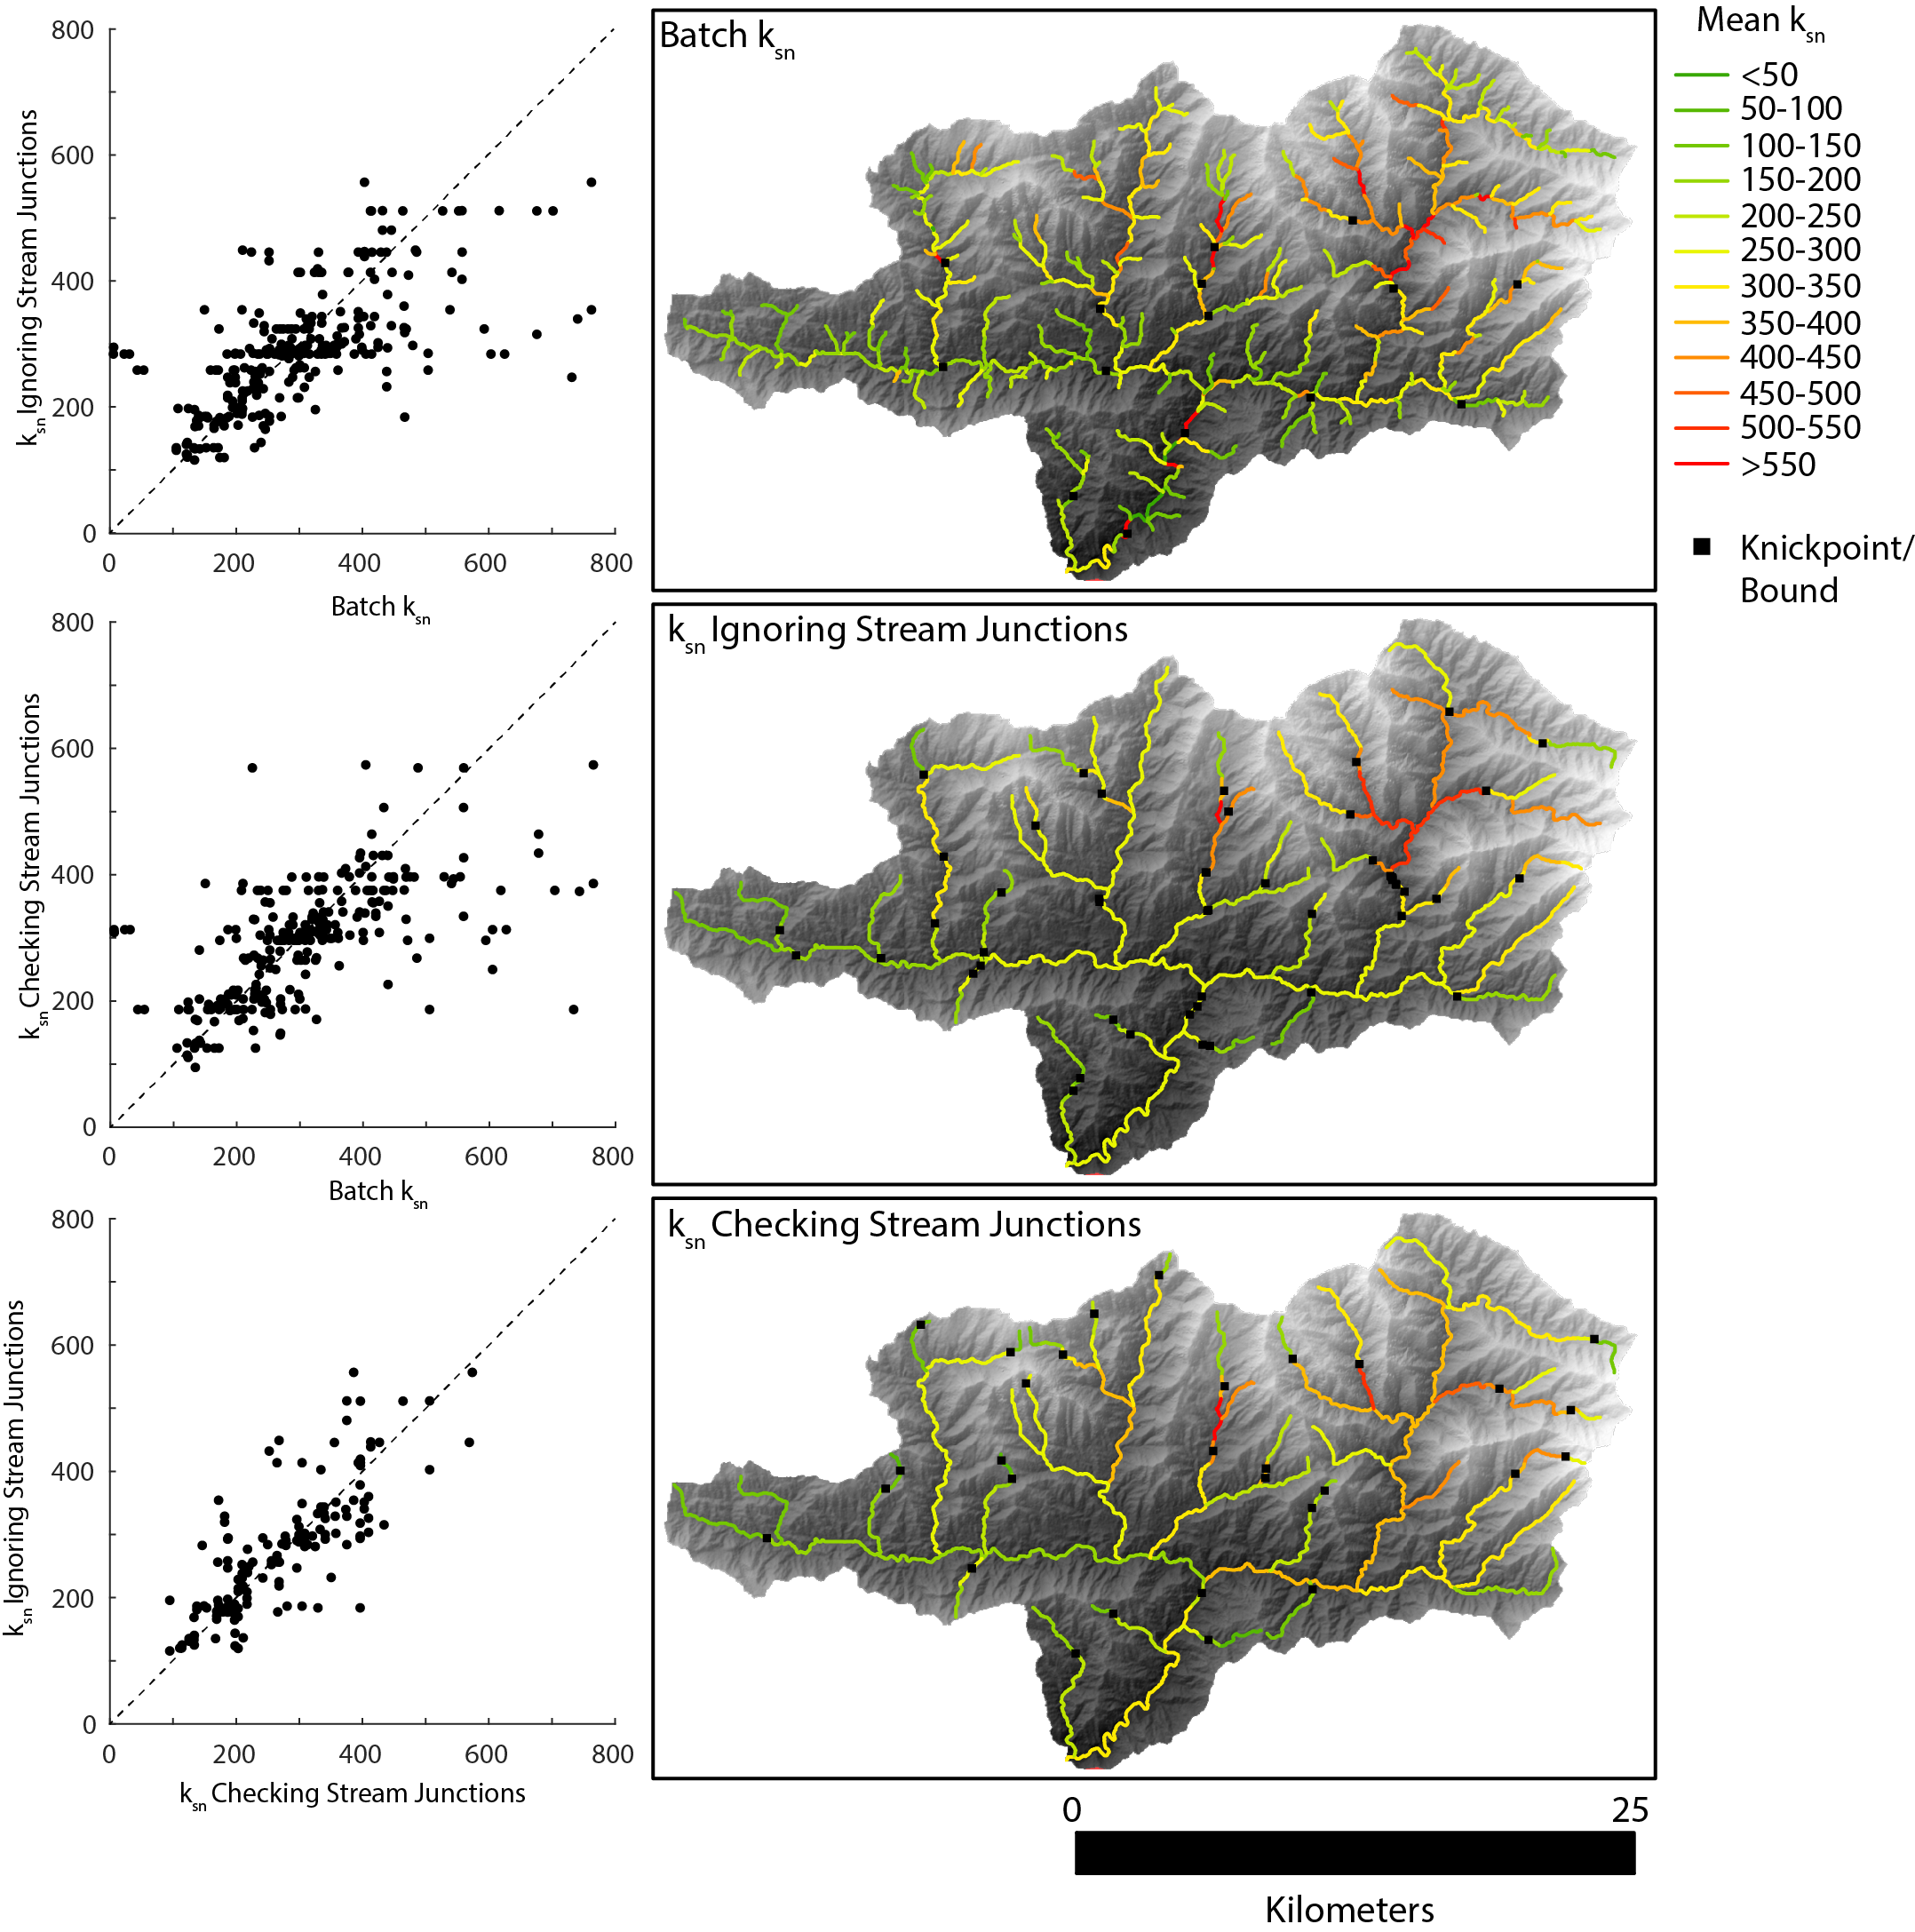
\includegraphics[width=16.5cm]{PNGs/Basin56_ksn_comparison.png}
	\caption{Comparison of \textit{k\textsubscript{sn}} values for Basin 56, calculated using the batch method (using \textit{KsnChiBatch})  or \textit{KsnProfiler} either ignoring or checking stream junctions.}
	\label{fig:ProfilerComp}
\end{figure}

\subsubsection{Defining the Minimum Threshold Area}
\paragraph{}By default, the \textit{KsnProfiler} function will use the stream network exactly as supplied, but there are several options for more precisely controlling the minimum threshold area for streams. The first option is to use \nameref{sec:FindThresh} to regenerate the stream network and use this new \textit{STREAMobj} as the input to \textit{KsnProfiler}. Alternatively, you can use a built in function of \textit{KsnProfiler} via the optional \textit{'redefine\_threshold'} parameter to choose the minimum threshold area on either a slope-area or $\chi$-elevation plot (Figure \ref{fig:ThreshSelect}).

 \begin{lstlisting}[language=Matlab]
% To redefine minimum threshold area for each stream chosen stream segment individually:
[~,~,~,~]=KsnProfiler(DEM,FD,A,S,'redefine_threshold',true);
\end{lstlisting}

\begin{figure}[H]
	\centering
	\begin{subfigure}{.5\textwidth}
		\centering
		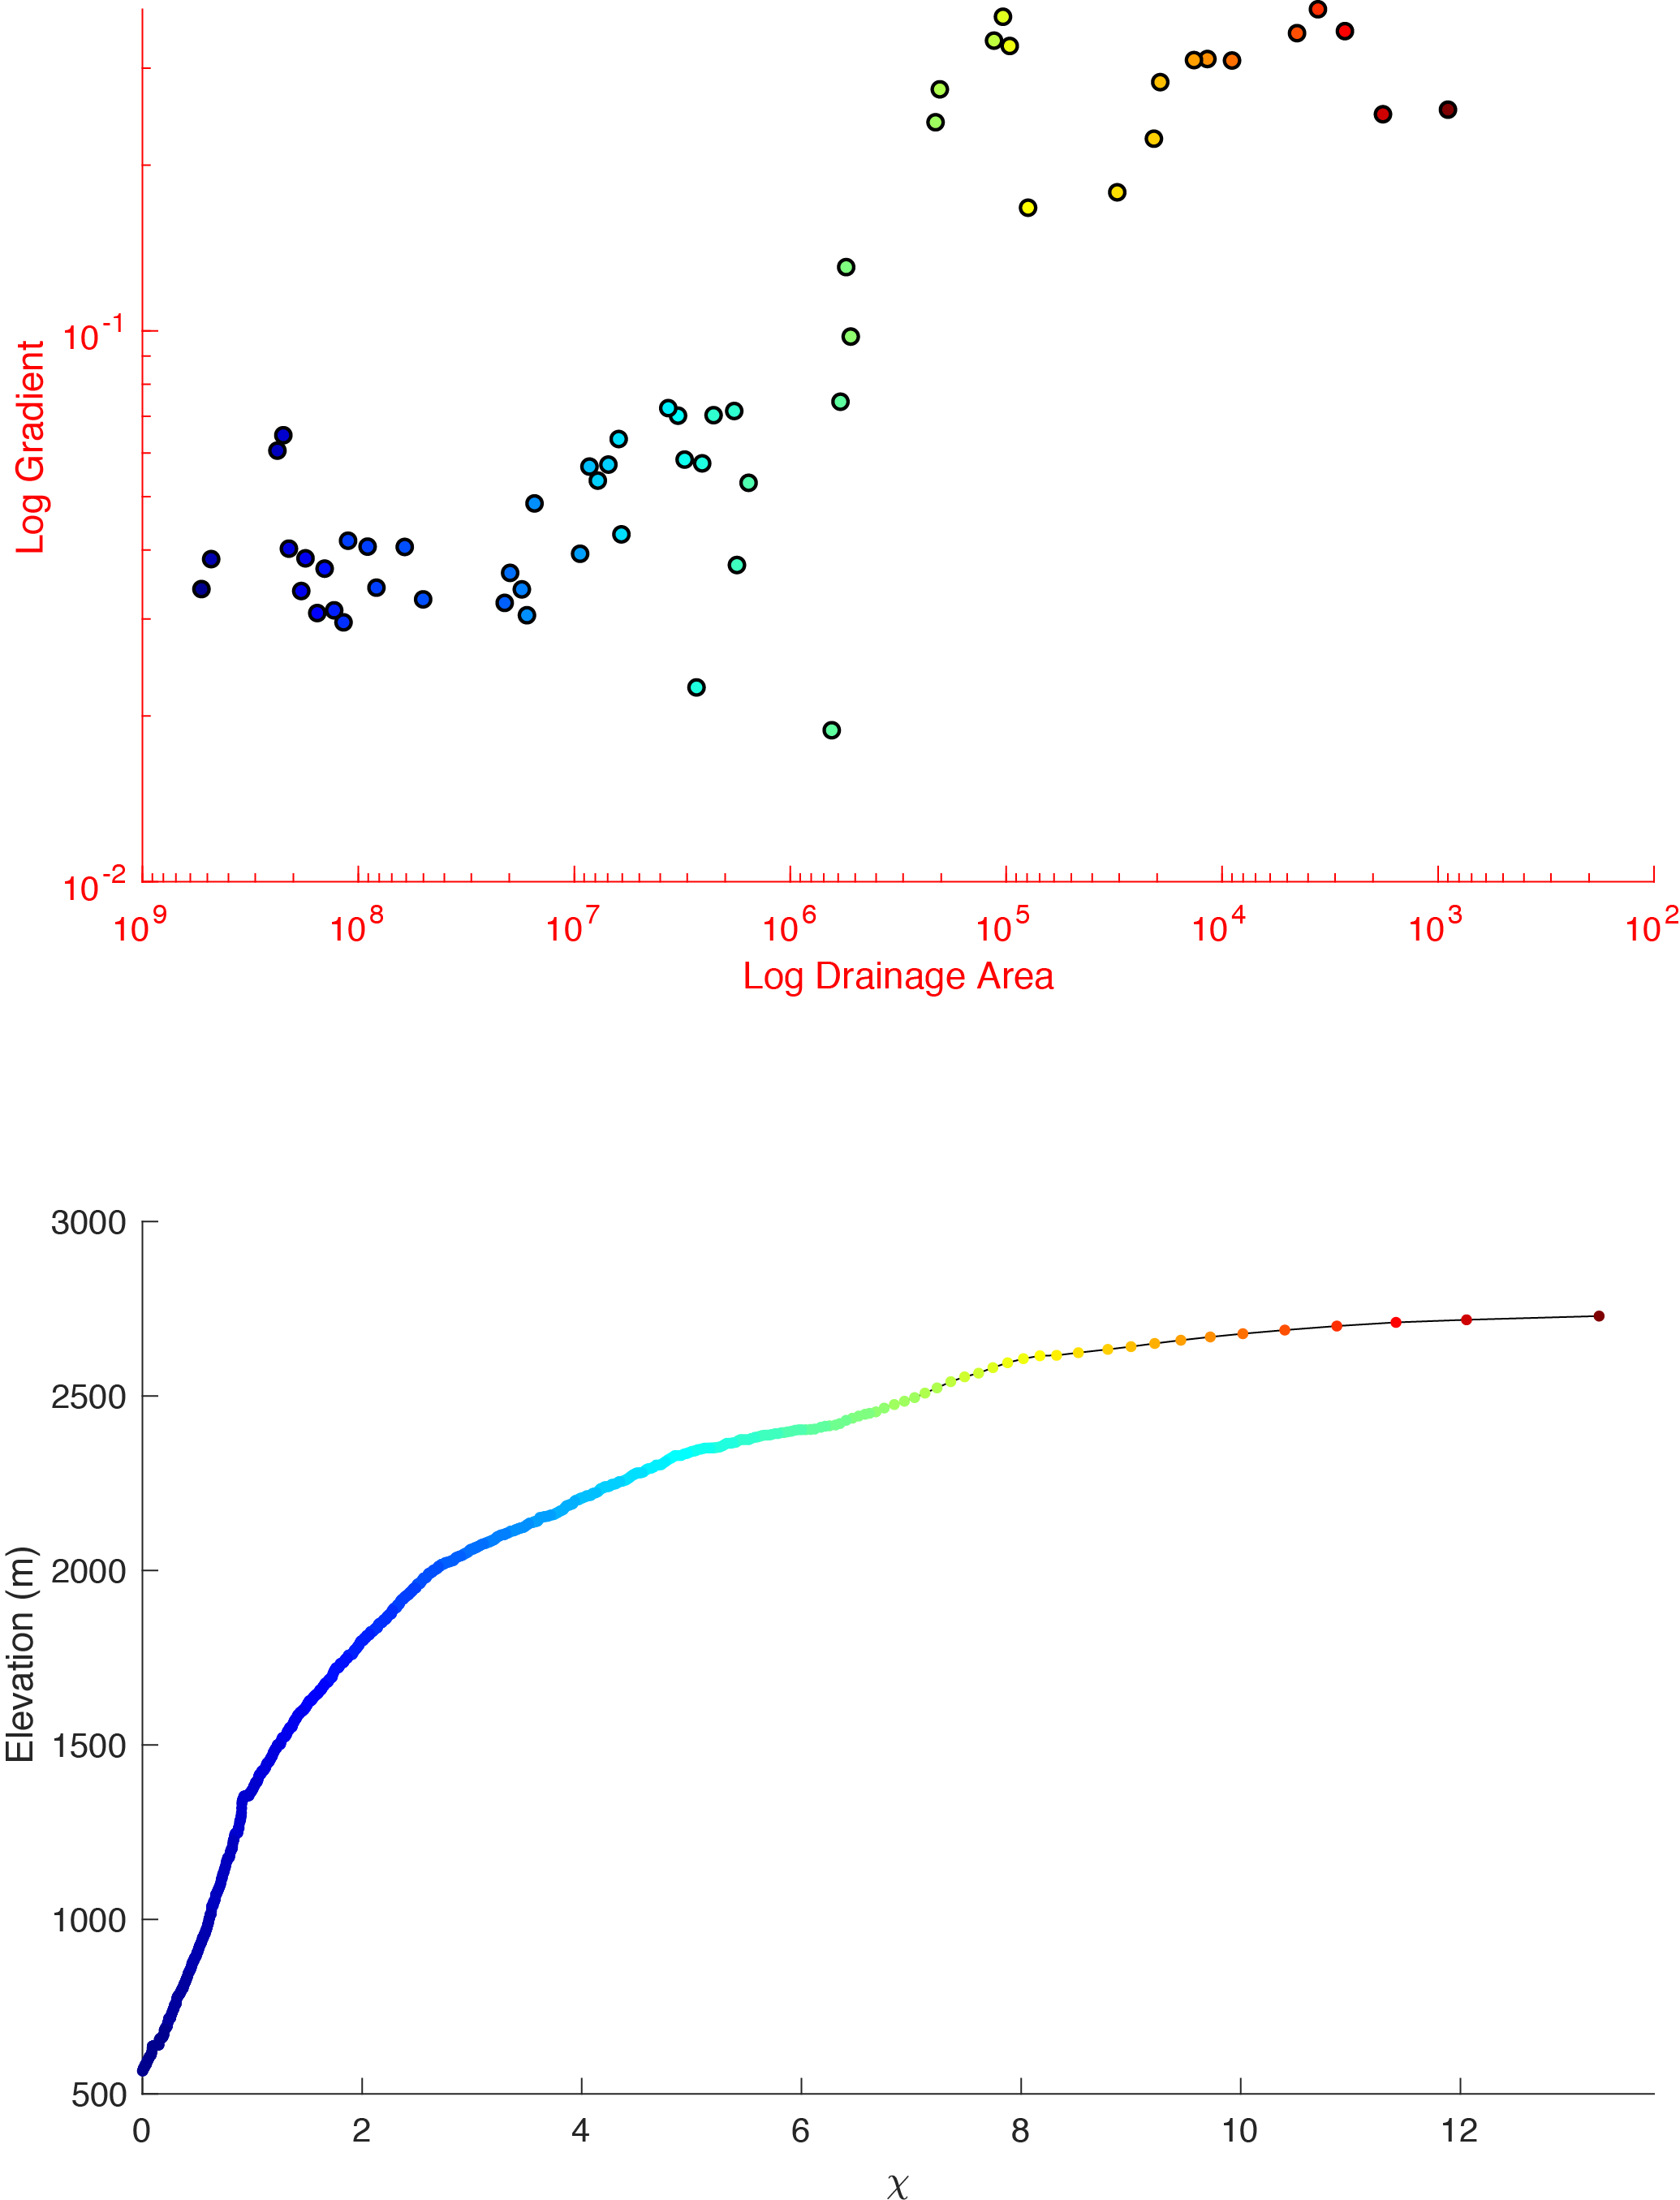
\includegraphics[width=.8\linewidth]{PNGs/B92_StreamThresh_9_prePick.png}
		\caption{Before threshold area selection}
		\label{fig:TSsub1}
	\end{subfigure}%
	\begin{subfigure}{.5\textwidth}
		\centering
		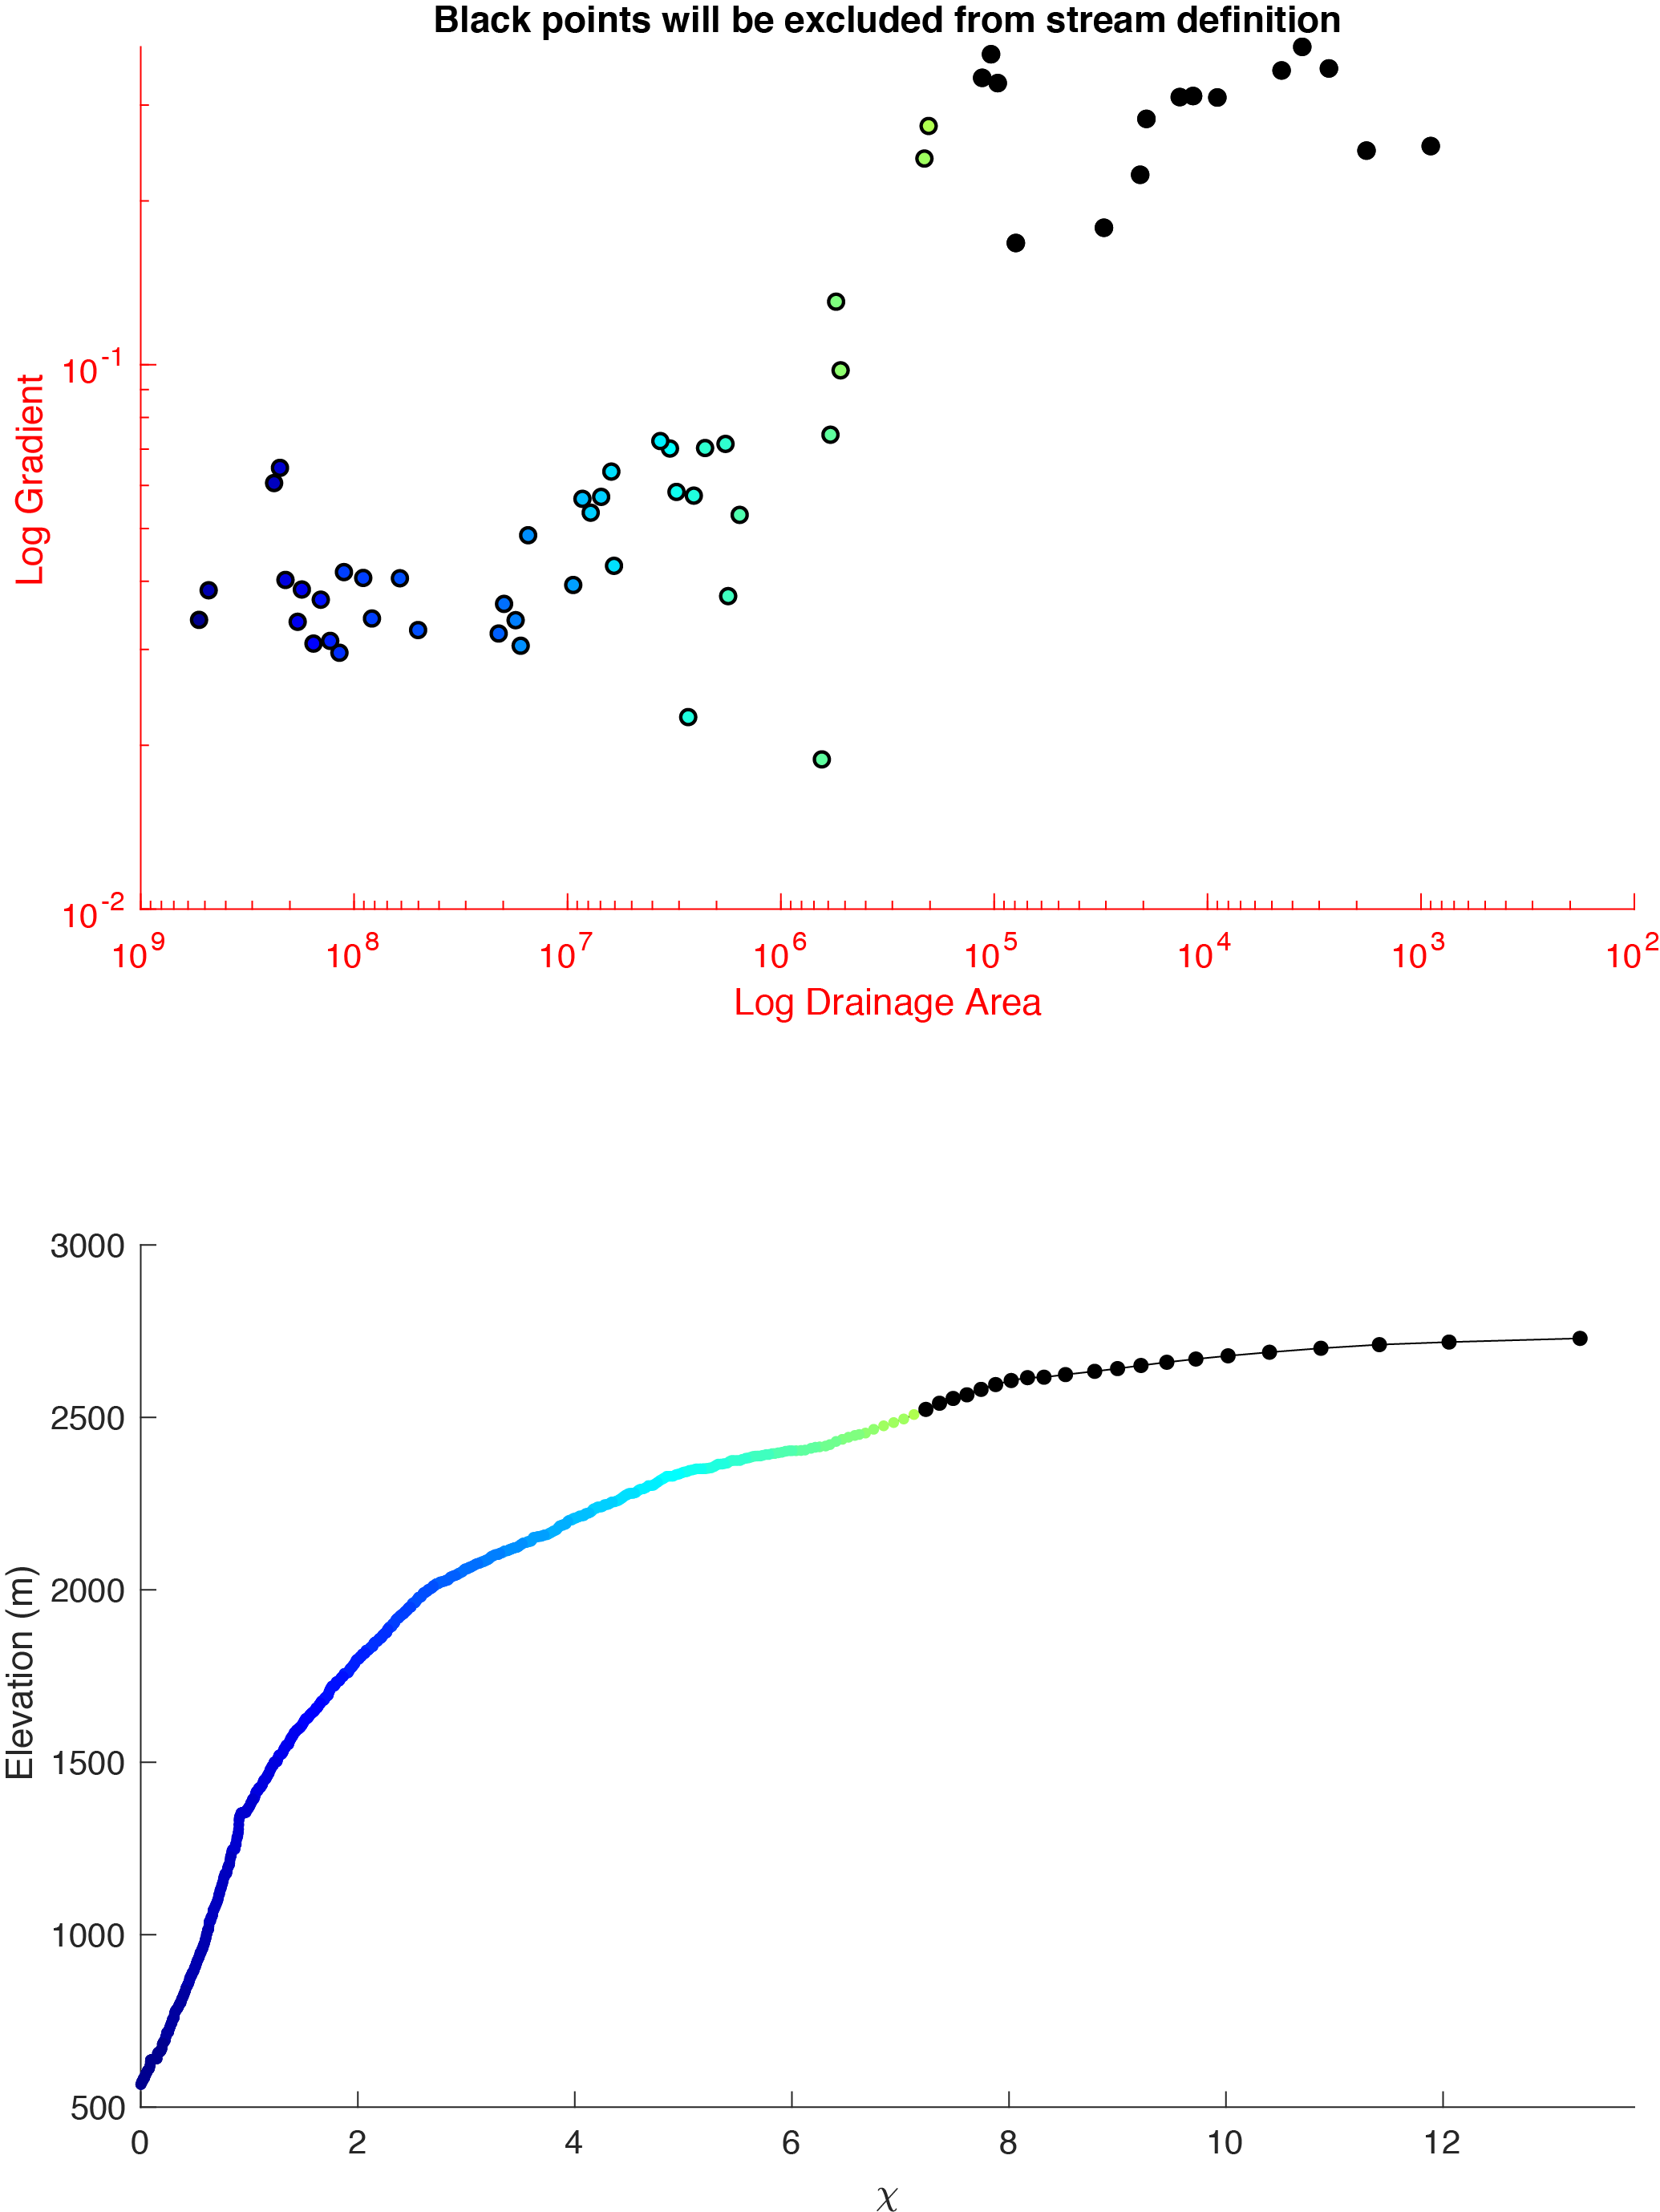
\includegraphics[width=.8\linewidth]{PNGs/B92_StreamThresh_9_postPick.png}
		\caption{After threshold area selection}
		\label{fig:TSsub2}
	\end{subfigure}
	\caption{Example of defining minimum threshold area on a slope-area plot using \textit{KsnProfiler}, black dots are portions of the stream network that will be excluded from channel definition.}
	\label{fig:ThreshSelect}
\end{figure}

\subsubsection{Restarting and Recovering from Errors}
\paragraph{}The \textit{KsnProfiler} function is designed to be very robust in case of errors (both actual errors and user error). Throughout the normal operation of the function, the user is able to redo any step in the stream selection or fitting processes. While the function is running, a temporary mat file is also saved that stores all the values necessary to restart if the code fails for some reason. A failed run can be restart by using the \textit{'restart'} optional parameter. The \textit{'restart'} option can also be used to pick up where you left off from a user terminated session (i.e. you indicated to the function that you were done, but subsequently decided you wanted to keep fitting streams). Whether you are restarting a run because of failure or simply picking up where you left off, you do not need to recreate the exact call to the function as the function also saves a record of all parameter values and uses these saved values during a restart run (note though that you still need to provide the required datasets).

\subsubsection{General Use}
\paragraph{}\textit{KsnProfiler} can be run either with a user provided reference concavity or in a mode where the best-fit concavity is found for each selected stream individually. Note that \textit{k\textsubscript{sn}} values can only be compared between streams if the same reference concavity is used, so it is generally recommended that unless you are explicitly only interested in the concavity of streams, that you leave the \textit{concavity\_method} set to the default \textit{ref} mode. Regardless of your choice for \textit{concavity\_method}, a best-fit concavity is calculated for each stream segment and is recorded in the outputs. Finding the best-fit concavity relies on the TopoToolbox \textit{chiplot} function, where this function searches for the concavity value that minimizes the difference between the true $\chi$-elevation relationship of the stream segment and a linear $\chi$-elevation relationship. During general use of \textit{KsnProfiler}, for any stream that is selected, you will be prompted to select segment boundaries on a plot (Figure \ref{fig:SegSelSub1}). These manually selected segment boundaries will be output as both a matlab array and a point shapefile. It should be noted that because the selection of these segments is manual, individual selections are not strictly reproducible. However, because the code restricts segment boundaries to stream nodes, there are a limited number of options for segment boundaries so in practice, while tedious, results for a given stream can be mostly reproduced (i.e. if you were trying to reproduce previous segment location choices).

\paragraph{}The exact construction of the plot will depend on a variety of optional input parameters. You can choose segment boundaries on either a $\chi$-elevation plot, a longitudinal profile plot, or a slope-area plot. In detail, regardless of the plot on which you choose to select segments, the calculation of best fit \textit{k\textsubscript{sn}} is performed on the $\chi$-elevation relationship for that segment. To ensure that the fit is not biased by the spacing of $\chi$ values that vary as a function of drainage area, the fit is performed on a spline interpolated version of the $\chi$-elevation relationship for the segment with equal point spacing in $\chi$. The function also produces a residual plot to aid in your assessment of the goodness of fit (Figure \ref{fig:ProfilerRes}).

\begin{figure}[H]
	\centering
	\begin{subfigure}{.5\textwidth}
		\centering
		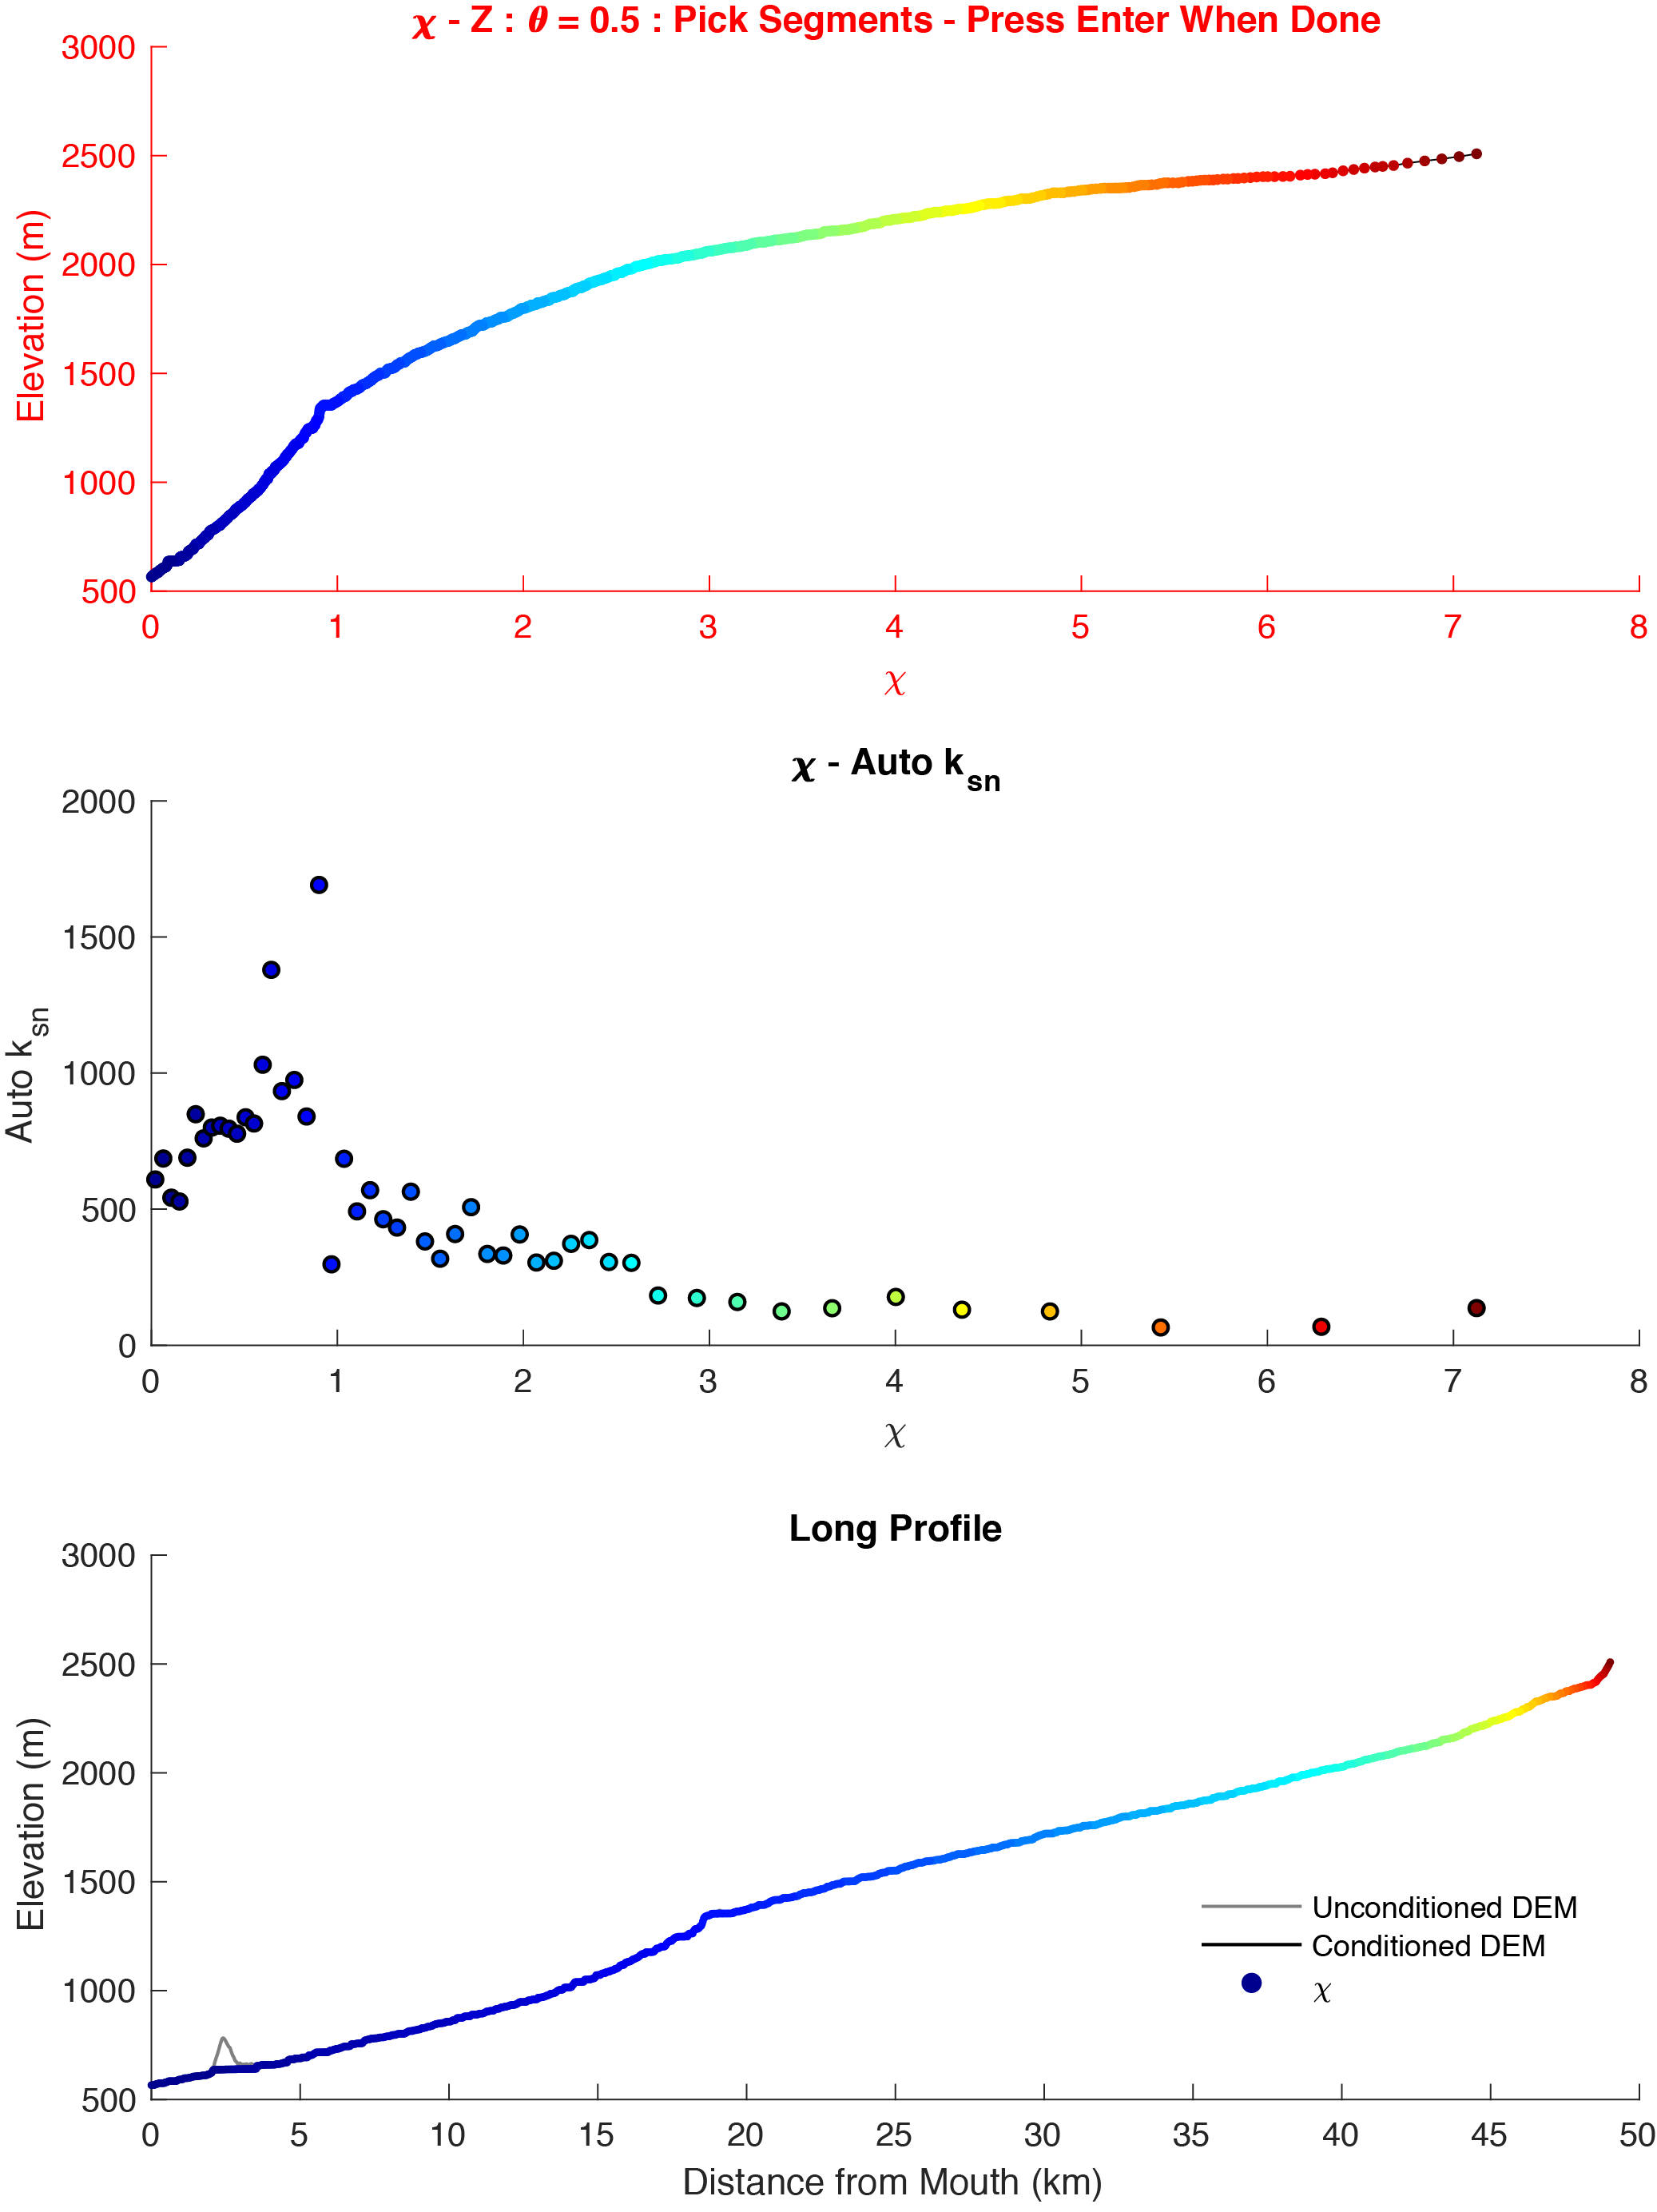
\includegraphics[width=.8\linewidth]{PNGs/B92_StreamFits_9_preFit.png}
		\caption{Main channel display before segment selection}
		\label{fig:SegSelSub1}
	\end{subfigure}%
	\begin{subfigure}{.5\textwidth}
		\centering
		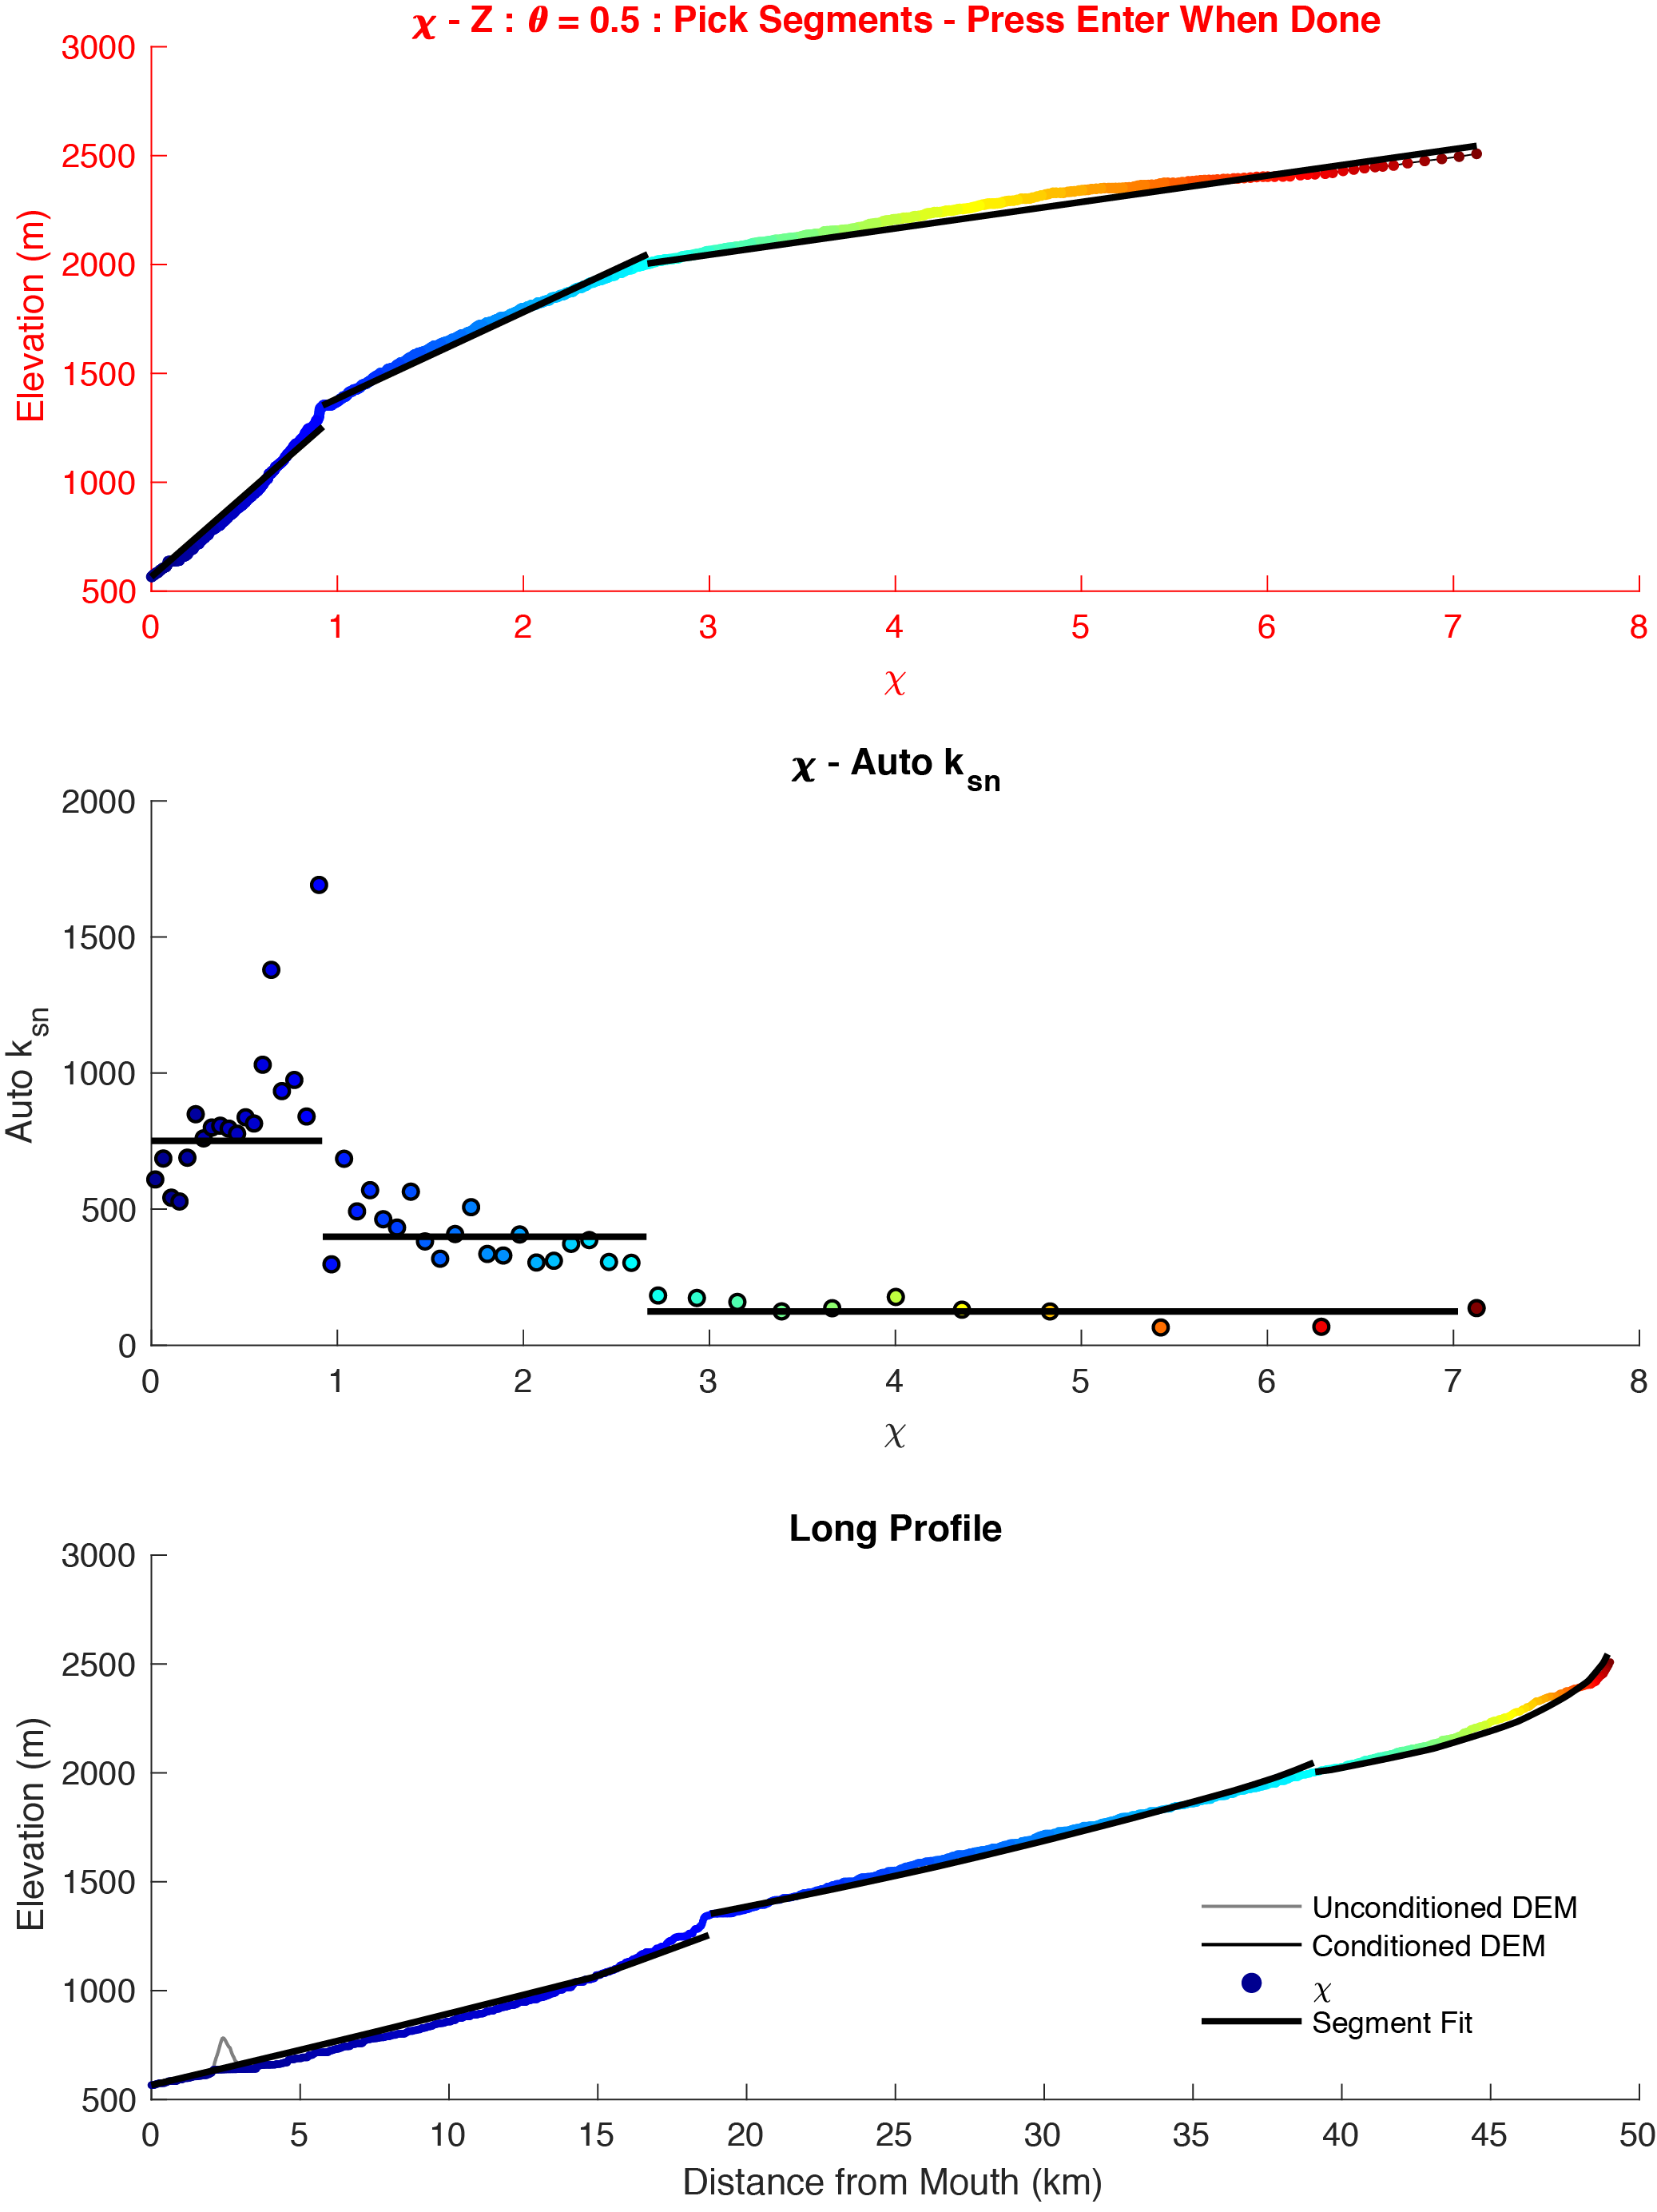
\includegraphics[width=.8\linewidth]{PNGs/B92_StreamFits_9_postFit.png}
		\caption{Main channel display after segment selection showing fit segments}
		\label{fig:SegSelSub2}
	\end{subfigure}
	\caption{Segment selection and fitting in \textit{KsnProfiler}}.
	\label{fig:SegSelect}
\end{figure}

\paragraph{}For all options, a plot of the batch \textit{k\textsubscript{sn}} vs a relevant quantity (i.e. either $\chi$, distance, or log area) will be displayed to aid you in picking out potential segments. The plot on which you need to make your selection will be highlighted with red axes, though for all options, the choice is recorded internally based on the position of the cursor in the x coordinate, so in the example (Figure \ref{fig:SegSelSub1}) you could click on segment boundaries based on values of $\chi$ on either the $\chi$-elevation or $\chi$-Auto \textit{k\textsubscript{sn}} plots and produce an accurate choice. The order in which you select segment boundaries doesn't matter and the outlet and channel head are automatically considered segment boundaries (i.e. you don't need to define these as segment boundaries). If you do not click anywhere in the plot, the function will treat the selected stream as one segment and fit a single \textit{k\textsubscript{sn}} value to the entire stream segment. Once you are done selecting segment boundaries, the function will find the best fit \textit{k\textsubscript{sn}} for each segment and display these (Figure \ref{fig:SegSelSub2}).

\begin{figure}[H]
	\centering
	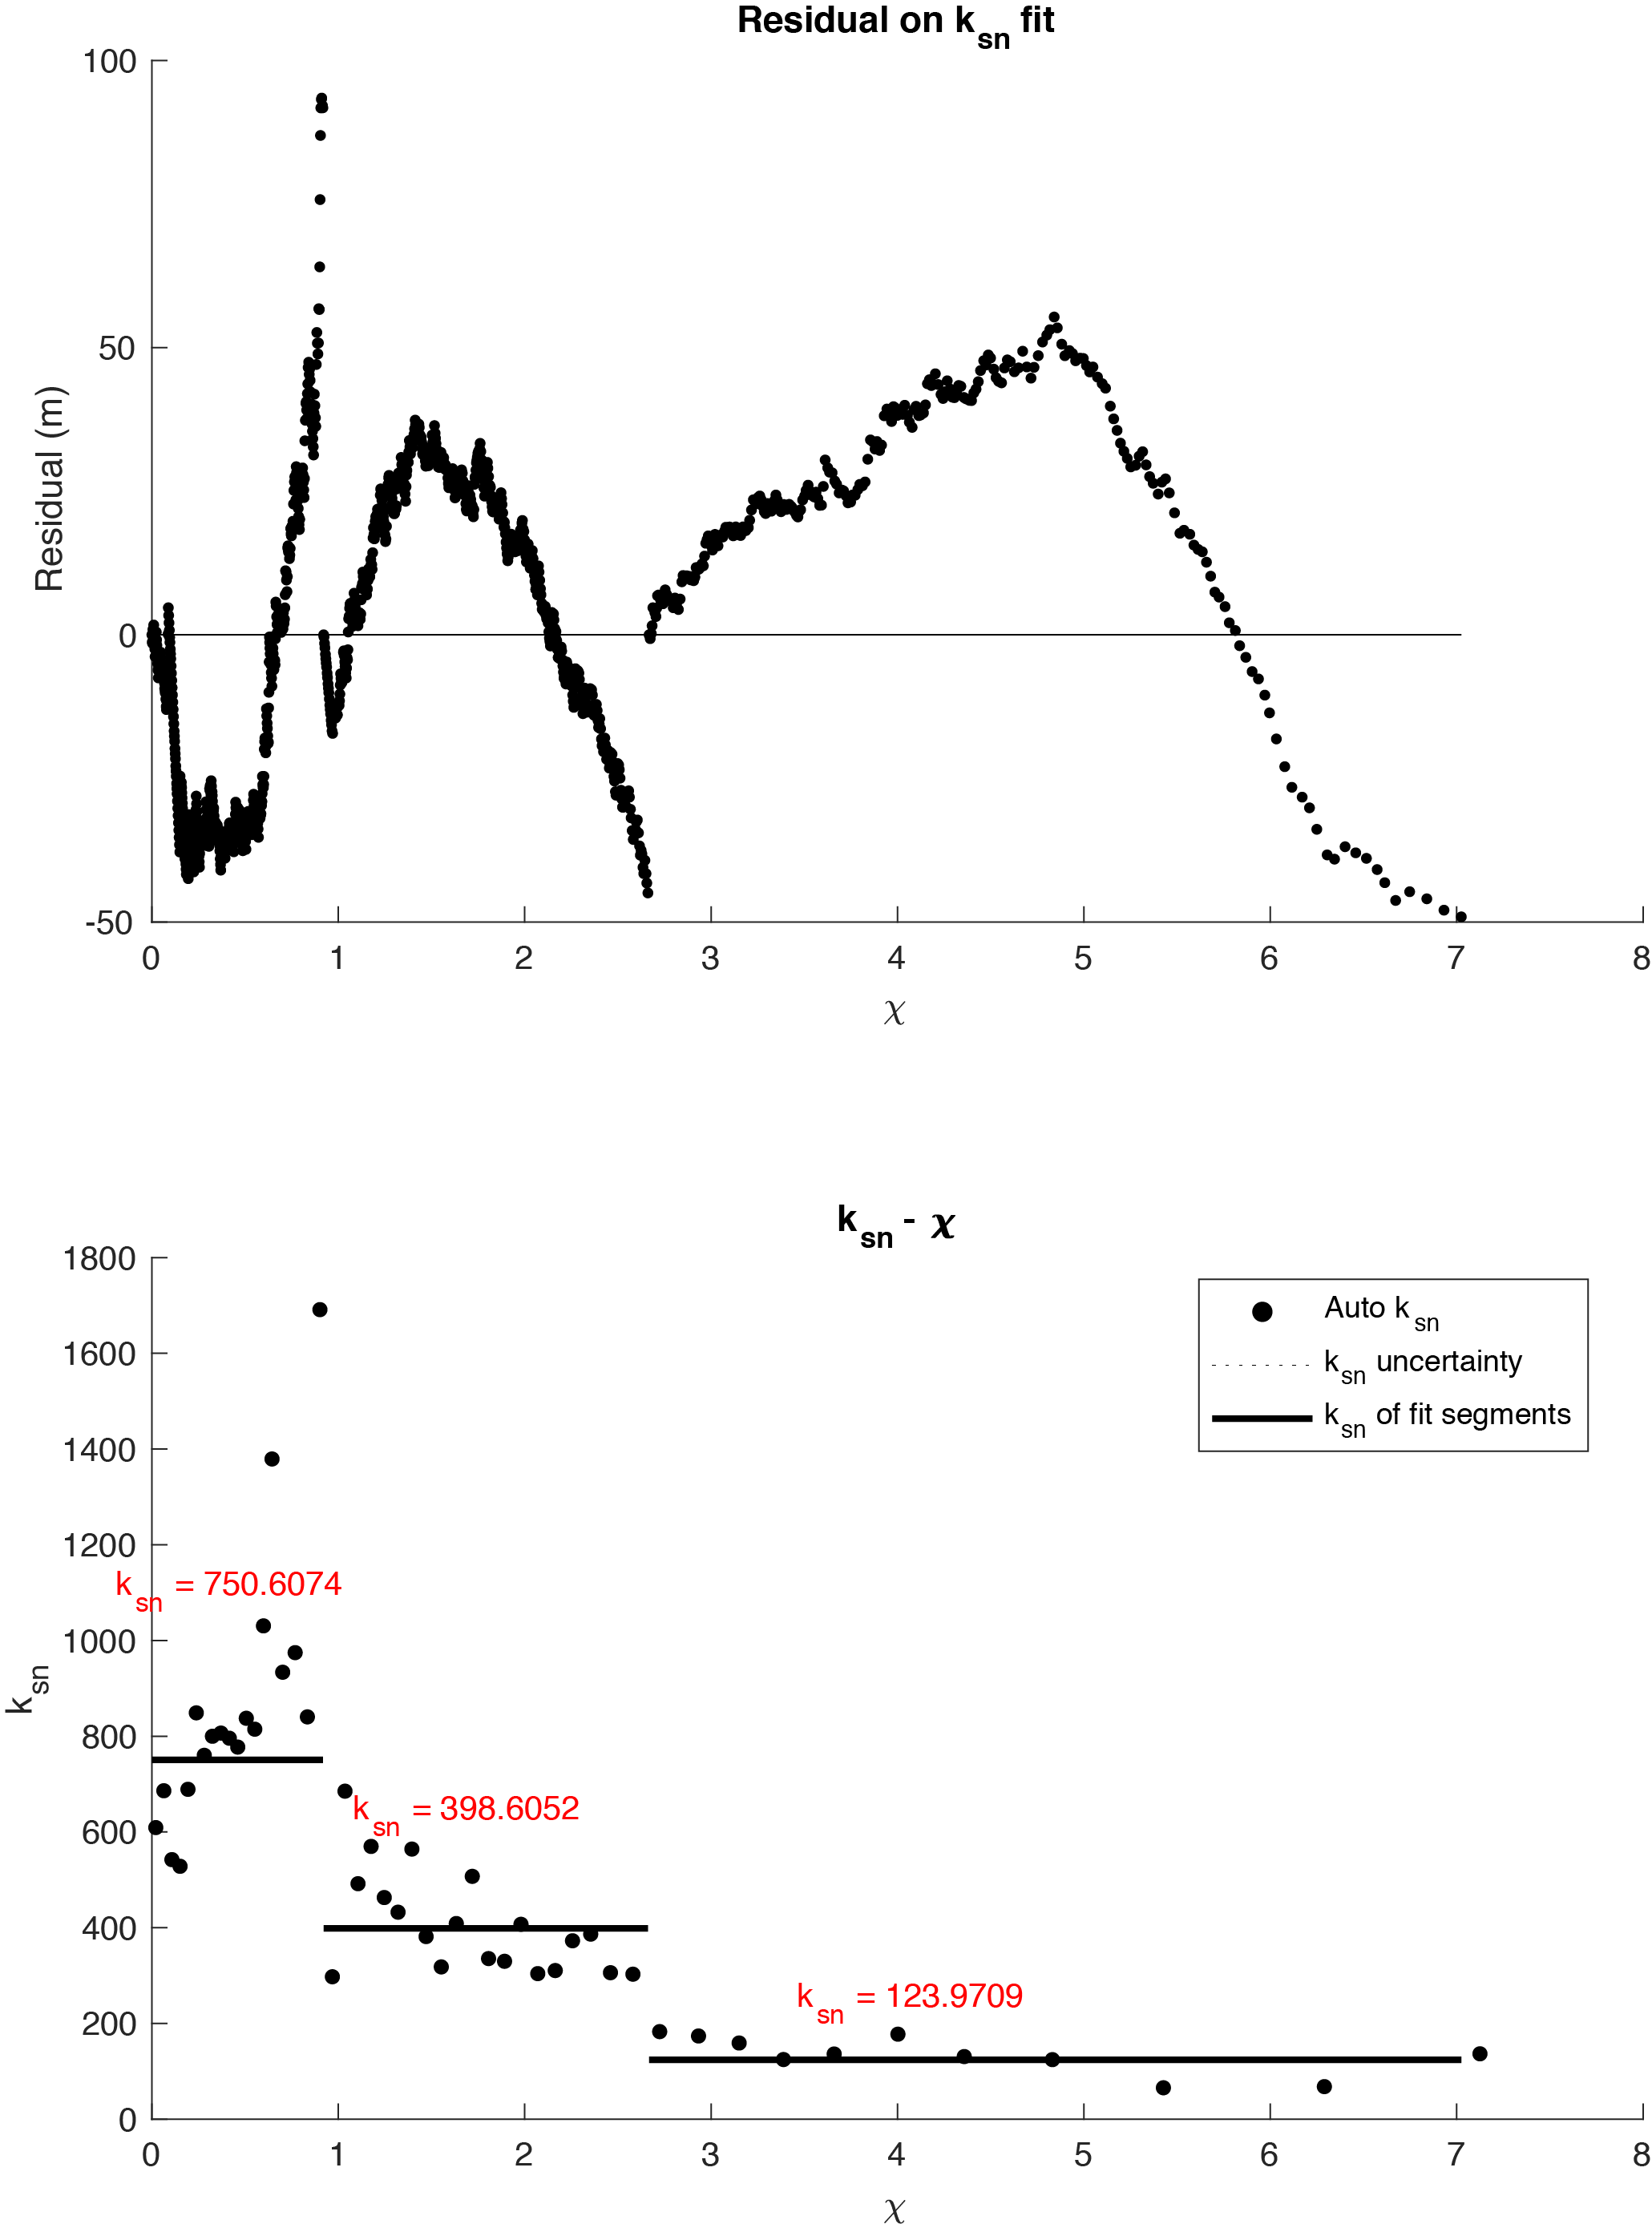
\includegraphics[width=10cm]{PNGs/B92_StreamRsds_9.png}
	\caption{Residuals on \textit{k\textsubscript{sn}} fit. Note that uncertainty values on the \textit{k\textsubscript{sn}} fits are calculated and plotted, but in this example, the uncertainties are small enough that they are not distinguishable from the main \textit{k\textsubscript{sn}} lines.} 
	\label{fig:ProfilerRes}
\end{figure}

\subsubsection{Outputs}
\paragraph{}The \textit{KsnProfiler} function produces four outputs to the workspace:

\begin{lstlisting}[language=Matlab]
[knl,ksn_master,bnd_list,Sc]=KsnProfiler(DEM,FD,A,S);
\end{lstlisting}

\noindent
 where \textit{knl} is an array of all stream locations with best fit \textit{k\textsubscript{sn}}, uncertainty values on this fit, concavity values, gradient, drainage area information, and reference ID numbers for the streams. This same output is also provided as a cell array, \textit{ksn\_master}, where individual streams are separated into cells. The segment boundaries are provided as an array of x, y, and z, locations in \textit{bnd\_list} and a \textit{STREAMobj} of the selected streams is provided as \textit{Sc}. Two shapefiles are produced, one as a polyline of the selected streams and containing all the information in the \textit{knl} output and a point shapefile of segment boundaries (i.e. knickpoints) is also produced (assuming segment boundaries were selected for any stream). Depending on the setup of your \textit{KsnProfiler} run, all of the plots generated during the fitting process may also be saved automatically.

\subsection{\textit{ClassifyKnicks}}
The \textit{ClassifyKnicks} is a companion function to \nameref{sec:KsnProfiler} that allows you to iterate through all segment boundaries selected during a \textit{KsnProfiler} run and provide a classification. This classification can either be numeric (e.g. 1, 2, 3, etc) or a character string (e.g., 'bound', 'slopebreak', 'knick', etc). If using character strings, these should be short (the shapefile format restricts entries in fields to 254 characters). The function will generate a new version of the knickpoint shapefile with this classification appended.

\subsection{\textit{AutoKsnProfiler}}
\paragraph{}Temporary

\subsection{\textit{EroGrid}} \label{sec:EroGrid}
\paragraph{}Temporary

%%%%%%%%
\section{Stream Junctions}
\subsection{\textit{JunctionAngle}} \label{sec:JAngle}
\paragraph{}Temporary

\subsection{\textit{InspectJunction}}
\paragraph{}The \textit{InspectJunction} function is provided mainly as a way of evaluating outputs of \nameref{sec:JAngle}. \textit{InspectJunction} expects the \textit{STREAMobj} used in the original call to \nameref{sec:JAngle} along with the \textit{'IX'} output from \nameref{sec:JAngle} and the number (i.e. the index of a particular junction as it appears in the output junction table) of a particular junction in question. Alternatively, you can provide an empty array to this number and manually select a junction to inspect on a map display of the stream network. 

\begin{figure}[H]
	\centering
	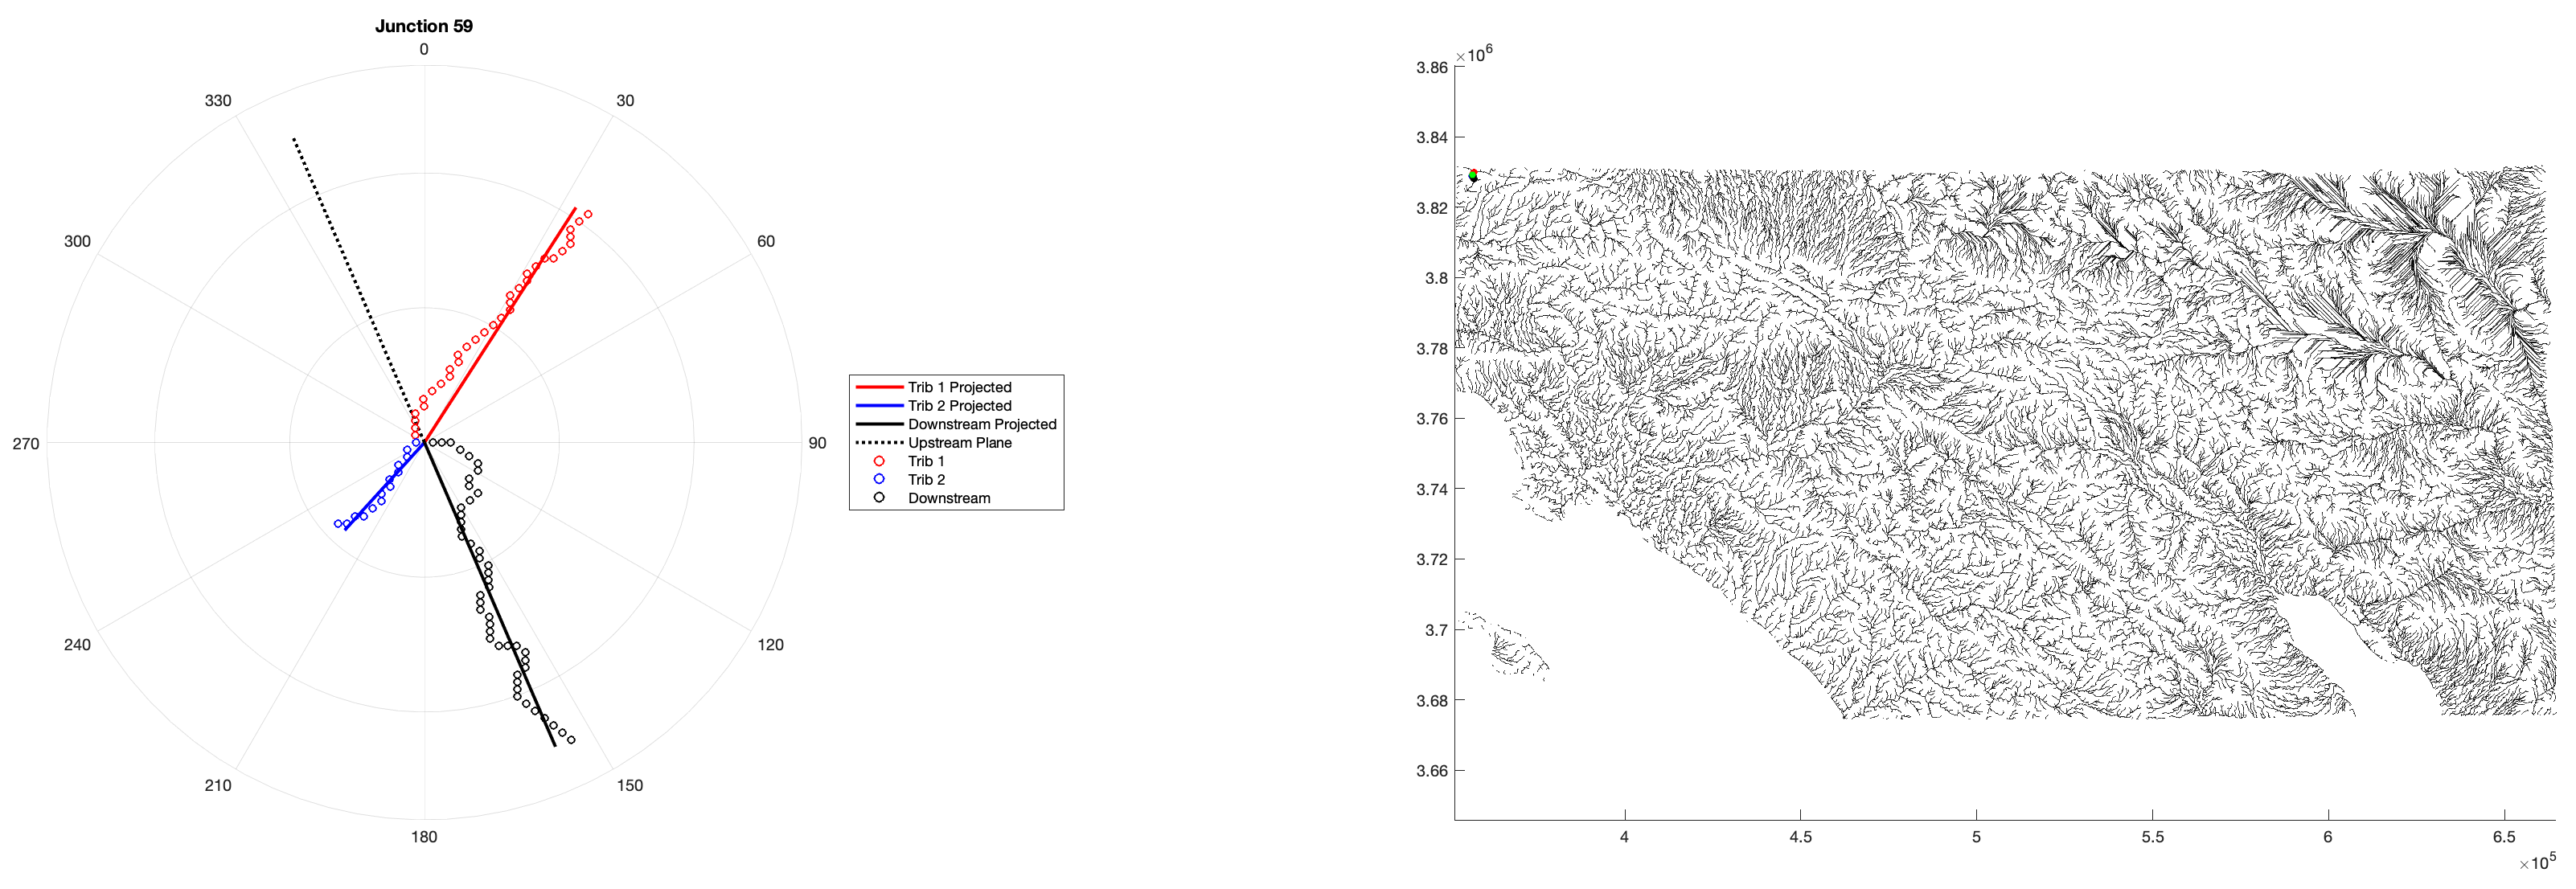
\includegraphics[width=16.5cm]{PNGs/InspectJunct.png}
	\caption{Details on the fit of a selected junction. Left plot is the selected portions of the stream showing the true stream path, as points, and the best fit lines used to calculate the junction angles, displayed in polar coordinates. The dashed line is the upstream projection of the downstream link, which is used to measure the pairs of junction angles reported in the junction table. Right plot is the map showing the location of the selected junction and the sections of streams in context.} 
	\label{fig:InspectJunc}
\end{figure}

\paragraph{}With the optional inputs to \textit{InspectJunction}, you can also manually change the length (either as stream length or number of nodes) over which the junction angels are fit to test the sensitivity of the junction angle to the fit distance. If no entries are provided to the optional \textit{'fit\_distance'} or \textit{'num\_nodes'}, the function will use the stream length selected during the original call to \nameref{sec:JAngle}, which will either be the single value supplied or the maximum value supplied if multiple fit distances were specified.

\subsection{\textit{JunctionLinks}}
\paragraph{}Temporary

%%%%%%%%
\section{Basin Selection}

\subsection{\textit{BasinPicker}} \label{sec:BsnPckr}
\paragraph{}The \textit{BasinPicker} function was originally designed to aid in the selection of sample locations for catchment averaged erosion rates (i.e. sand samples for  \textsuperscript{10}Be analysis), but can also be used as an interactive gateway to the \nameref{sec:PrcRvBsn} function. \textit{BasinPicker} takes the standard inputs:

\begin{lstlisting}[language=Matlab]
[Outlets]=BasinPicker(DEM,FD,A,S);
\end{lstlisting}

\noindent
 and displays the DEM along with a map of local relief (radius of relief can be specified with optional \textit{'rlf\_radius'} parameter) and the provided stream network and prompts the user to choose a pour point / river mouth. The function will first confirm that you choose the correct portion of the stream network and then, if you answer in the affirmative, will display the plot of the $\chi$-elevation and longitudinal profile for the streams within the selected basin and will also print out the mean local relief, mean channel steepness, and drainage area of the selected basin. The function will then ask if you wish to keep or discard this basin from the running list of outlets. The rationale being that if you are using this for sample site selection, you may not want to include basins that have major knickpoints, are below/above a particular drainage area, or do not meet some user defined morphometric criteria. 

\paragraph{}After each confirmed selection, \textit{BasinPicker} will append this to an \textit{'Outlets.mat'} file. If you run \textit{BasinPicker} when an \textit{'Outlets.mat'} file is in the active directory (or on your path), the code will attempt to populate the map with previous outlet selections. If you have already calculated local relief for your area of interest, you can skip the recalculation by providing a \textit{GRIDobj} of local relief to the optional \textit{'rlf\_grid'} parameter. You can also provide an additional \textit{GRIDobj} if you wish to consider an additional gridded dataset in selecting basin outlet locations:

\begin{lstlisting}[language=Matlab]
% Providing a precomputed relief grid
[Outlets]=BasinPicker(DEM,FD,A,S,'rlf_grid',RLF);
% Providing an extra grid
PRECIP=GRIDobj('/Users/aforte/GISdata/precip.tif');
[Outlets]=BasinPicker(DEM,FD,A,S,'extra_grid',PRECIP);
\end{lstlisting}

\noindent
The provided extra grid does not need to the same dimensions as the input DEM, etc, but it does need to be in the same projection. If you provide an extra grid, the mean values of this grid within the selected basin(s) will also be displayed in the plots. 

\paragraph{}In some instances, you may be selecting basins that are upstream of specific locations, e.g. if you want to calculate basin averaged statistics for watersheds above detrital sample sites for which you have GPS coordinates. Very often, the true location of streams, and samples from them, will be slightly different than the location of the stream that results from flow routing, such that just using the GPS location of a sample site will result in incorrect basin selection, requiring a laborious process of nudging true locations to lie on stream lines. This process can be sped by providing the list of coordinates to the optional \textit{'refine\_positions'} argument in \textit{BasinPicker}. After providing these locations, the code will iterate through each position and show its location on the main map but also the location of the sample and the stream network in a separate zoomed in window, allowing you to precisely reposition the river mouth. The amount of zoom is controlled by the \textit{'window\_size'} parameter, where you can specify the size of the zoomed in window in kilometers. For example:

\begin{lstlisting}[language=Matlab]
% Load a shapefile containing your GPS coordinates
ms=shaperead('my_gps_points.shp');
% Extract the X and Y coordinates and put them into a m x 2 array
gps_pnts=[[ms.X] [ms.Y]]
% Run BasinPicker with window size of the zoomed window set to 2 km
[Outlets]=BasinPicker(DEM,FD,A,S,'refine_positions',gps_pnts,'window_size',2);
\end{lstlisting}

%%%%%%%%
\section{Basin Average Maps and Plots}

\paragraph{}A major part of the \textit{Topographic Analysis Kit} are tools designed for efficient selection and analysis of basin averaged data.

\subsection{\textit{ProcessRiverBasins}} \label{sec:PrcRvBsn}

\subsubsection{Basic Operation}
\paragraph{}The workhorse function within the broader basin averaging set of tools is \textit{ProcessRiverBasins}. \textit{ProcessRiverBasins} was initially designed to efficiently clip out a series of watersheds from a larger DEM for use in ArcGIS, but has expanded much beyond that capability. The basic operation of \textit{ProcessRiverBasins} requires the standard inputs along with a list of river mouths above which watersheds will be extracted. This list of river mouths can be provided as a Matlab array, e.g. the list of outlets output from \nameref{sec:BsnPckr} is a valid input for \textit{ProcessRiverBasins}:

\begin{lstlisting}[language=Matlab]
% Using output of BasinPicker to run ProcessRiverBasins
load('Outlets.mat','Outlets');
ProcessRiverBasins(DEM,FD,A,S,Outlets,'basin_dir');
\end{lstlisting}

\noindent
where \textit{'basin\_dir'} is the name of a folder (or full path of a folder) in which to store all of the datafiles that will be produced during a \textit{ProcessRiverBasins} run. If the provided folder name does not exist, the function will create the folder. You do not have to use \nameref{sec:BsnPckr} to generate the river mouth input, you only need to provide an array of x and y locations with ID numbers. Alternatively, you can provide a point shapefile where individual points are placed in locations where you wish there to be river mouth and each point has an identifying number (you can use the default ID number that ArcGIS will generate, but it is recommended that you make a separate field in your shapefile and manually provide ID numbers) :

\begin{lstlisting}[language=Matlab]
% Using a point shapefile to run ProcessRiverBasins
ProcessRiverBasins(DEM,FD,A,S,'points_shape.shp','basin_dir');
\end{lstlisting}

\noindent
As a caution, if you are going to use a GIS program (e.g. ArcGIS or QGIS) to select river mouth locations, it is strongly recommended that you use the stream shapefile output from \nameref{sec:MakeStreams} as opposed to a stream network generated using flow routing in the GIS program of your choice. This is because flow routing algorithms vary slightly and thus  absolute stream locations vary. Prior to the clipping process, \textit{ProcessRiverBasins} will snap the provided river mouths to the provided stream network, so accidental selection of the wrong basin is possible if the selection of river mouths was done on an alternative stream network shapefile. Similarly, if you are using \textit{ProcessRiverBasins} to clip out and calculate statistics on true sample locations (e.g. locations of detrital sediment samples as recorded by a GPS), it is again recommended that you ensure that these locations lie on the correct portion of the stream network generated by \nameref{sec:MakeStreams} or incorrect basins may be clipped. \textbf{This may require moving true locations to lie on the correct flow routed stream!} For an easy way to do this, see the \textit{'refine\_positions'} option in \nameref{sec:BsnPckr}.

\paragraph{}A final option for fully automated selection of river mouths allows you to provide an elevation as the river mouth parameter. This will place river mouths on the stream network at every location the stream network drops below this provided elevation:

\begin{lstlisting}[language=Matlab]
% To create basins with outlets above 1000 meters elevation
ProcessRiverBasins(DEM,FD,A,S,1000,'basin_dir');
\end{lstlisting}

\paragraph{}River mouths provided to \textit{ProcessRiverBasins} can be non-nested or nested as each basin is processed independently of all other basins. If your goal is to simply to generate a large dataset of arbitrary small basins within a landscape, we recommend placing river mouths at strategic locations (e.g. where streams exit a mountain range, Figure \ref{fig:BasinsComp}) and use \textit{ProcessRiverBasins} to process these large basins and then use \nameref{sec:SbDvdBsn} to automatically subdivide basins as opposed to manually selecting large numbers of nested, sub-basins.

\paragraph{}The \textit{ProcessRiverBasins} function will use the river mouth locations to extract basins. For each basin there will be a Matlab .mat file which will contain its own basic TopoToolbox files along with various derived quantities, e.g. geographic data structure of \textit{k\textsubscript{sn}} using a reference concavity, geographic data structure of \textit{k\textsubscript{sn}} using a best-fit concavity for that watershed (remember that \textit{k\textsubscript{sn}} values calculated with different concavities are not comparable when considering these outputs!), hypsometry and hypsometric integral for the basin, slope map, and statistics (mean, standard deviation or standard errors) on the majority of these quantities. See the \nameref{sec:UndOuts} for a complete list of outputs stored within the .mat file. Because it is time consuming, local relief is not calculated by default, but you can specify that you wish to calculate relief at a variety of radii using the \textit{'calc\_relief'} and \textit{'relief\_radii'} parameters:

\begin{lstlisting}[language=Matlab]
% Calculate relief with a radius of 2500 m for all basins
ProcessRiverBasins(DEM,FD,A,S,Outlets,'basin_dir','calc_relief',true,'relief_radii',2500);
% Calculate relief with at 1000, 2500, and 5000 m radii for all basins
ProcessRiverBasins(DEM,FD,A,S,Outlets,'basin_dir','calc_relief',true,'relief_radii',[1000 2500 5000]);
\end{lstlisting}

\paragraph{}If relief is calculated, statistics on these relief grids are also calculated. For each basin, a single .mat file is saved in the specified directory. The naming convention for these files is \textit{'Basin\_\#\_Data.mat'} where \# is the ID number in the river mouth input for a given basin. It is important that you do not change the names of these files as this will break other functions that use these as inputs. By default, files suitable for use in a GIS program are not generated for each basin. You can have the function do this automatically for all basins by setting the optional \textit{'write\_arc\_files'} to true or manually by using \nameref{sec:Mat2Arc} for the desired basins.

\subsubsection{Extra Grids}
\paragraph{}You can also provide an arbitrary number of extra grids to have \textit{ProcessRiverBasins} clip and calculate basin averaged statistics for these grids. These extra grids do not need to be the same dimensions or cellsize as the input DEM, but they do need to be in the same coordinate system and projection. Also, if any provided extra grids are smaller than the DEM and any selected basin includes areas that are not covered by the extra grid, this will produce biased statistics. Extra grids are provided to the \textit{ProcessRiverBasins} function as a 2 column Matlab cell array where the first column contains the \textit{GRIDobj} and the second column includes a name for this grid in conjunction with the \textit{'add\_grids'} parameter:

\begin{lstlisting}[language=Matlab]
% To run ProcessRiverBasins and include two extra grids
% Create the two GRIDobjs from data of interest
PRECIP=GRIDobj('/Users/aforte/GISdata/precip.tif');
NDVI=GRIDobj('/Users/aforte/GISdata/ndvi_grid.tif');
% Make an empty cell array
AG=cell(2,2);
% Populate cell array with necessary data 
% Note that location in cell arrays are referenced with curly brackets
AG{1,1}=PRECIP;
AG{1,2}='precip';
AG{2,1}=NDVI;
AG{2,2}='ndvi_val';
% Run ProcessRiverBasins
ProcessRiverBasins(DEM,FD,A,S,Outlets,'basin_dir','add_grids',AG);
\end{lstlisting}

\noindent
As a note, it is not recommended that you provide a local relief grid as an extra grid, but rather use the \textit{'calc\_relief'} option. The reason for this is twofold, 1) because local relief is calculated with a moving window, simply clipping out watersheds from a larger local relief raster will bias the statistics within the clipped watersheds as edge pixels will be influenced by neighboring basins and 2) subsequent codes explicitly look for the relief datasets in \textit{ProcessRiverBasins} outputs to determine behaviors. 

\paragraph{Note for Compiled Versions:} If you are running the compiled version of \textit{ProcessRiverBasins}, the procedure for adding extra grids is slightly different. Instead of directly providing the extra grids to \textit{ProcessRiverBasins}, you must first use the \nameref{sec:PrepAdd} function to prepare a .mat file containing these extra grids, the name of which is then provided to the compiled \textit{ProcessRiverBasins} function.

\subsubsection{Categorical Grids} \label{sec:PRB_ACG}
\paragraph{}Some data that you may want to include in ProcessRiverBasins is not natively supported as a \textit{GRIDobj}, specifically non-numeric data stored in polygonal shapefiles, e.g. units from a geologic map or vegetation types. You can provide this data as a usable input to ProcessRiverBasins via the optional \textit{'add\_cat\_grids'} parameter and with the help of the \nameref{sec:CatGrid} function. The input to the \textit{'add\_cat\_grids'} parameter is expected as a 3 column Matlab cell array, where the first column is the \textit{GRIDobj}, the second column is the lookup table (both of these are generated by \textit{CatPoly2GRIDobj}), and a name for the grid:

\begin{lstlisting}[language=Matlab]
% To run ProcessRiverBasins an additional categorical grid
% Generate the categorical grid and lookup table with CatPoly2GRIDobj
[GEO,geo_table]=CatPoly2GRIDobj(DEM,'geo_polygons.shp','PTYPE');
% Make an empty cell array
ACG=cell(1,3);
% Populate cell array with necessary data
ACG{1,1}=GEO;
ACG{1,2}=geo_table;
ACG{1,3}='rock_type';
% Run ProcessRiverBasins
ProcessRiverBasins(DEM,FD,A,S,Outlets,'basin_dir','add_cat_grids',ACG);
% For simple inputs like above, you can do most of this in one line after generating GEO and geo_table with CatPoly2GRIDobj
ProcessRiverBasins(DEM,FD,A,S,Outlets,'basin_dir','add_cat_grids',{GEO geo_table 'geology'});
\end{lstlisting}

\noindent
As with extra grids, more than one categorical grid can be provided, simply add additional rows to the input cell array. The remaining functions in this section all are either designed to operate on the products of \textit{ProcessRiverBasins} or serve as helper functions for \textit{ProcessRiverBasins}, e.g. \nameref{sec:CatGrid}. Because it is assumed that mean values of a category are not meaningful, the mode category value for each basin is found and used as the statistic. The function also calculates the number of pixels of each basin that belong to each category and saves this within the outputs.

\paragraph{Note for Compiled Versions:} If you are running the compiled version of \textit{ProcessRiverBasins}, the procedure for adding categorical grids is slightly different. Instead of running \nameref{sec:CatGrid} and providing the result directly to \textit{ProcessRiverBasins}, you must instead use the \nameref{sec:PrepCat} function to prepare a .mat file containing these categorical grids, the name of which is then provided to the compiled \textit{ProcessRiverBasins} function.

\subsubsection{Understanding Outputs} \label{sec:UndOuts}
\paragraph{}Each basin .mat file (or sub-basin file if considering the outputs of the related \nameref{sec:SbDvdBsn}) contains a lot of outputs. For the most part, subsequent functions are designed to use and process these basin files, but in some cases you may wish to use products directly so we provide a list of all the outputs and a brief description of each below.

\begin{enumerate}
	\item Default outputs regardless of optional parameters or datasets:
	\begin{itemize}
		\item \textit{RiverMouth} - array storing the x and y coordinate and ID number of the outlet of the basin
		\item \textit{DEMcc} - clipped \textit{GRIDobj} of the hydrologically conditioned DEM of the basin
		\item \textit{DEMoc} - clipped \textit{GRIDobj} of the original DEM of the basin
		\item \textit{out\_el} - scalar value of elevation of the outlet of the basin in map units
		\item \textit{drainage\_area} - scalar value of the drainage area of the basin in square kilometers
		\item \textit{hyps} - two column array of the hypsometry of the basin, first column is relative frequencies, second column is elevation
		\item \textit{FDc} - clipped \textit{FLOWobj} of the basin
		\item \textit{Ac} - clipped \textit{GRIDobj} of the flow accumulation raster of the basin
		\item \textit{Sc} - \textit{STREAMobj} containing the full stream network of the basin
		\item \textit{SLc} - \textit{STREAMobj} containing the largest connected full stream network of the basin (should be identical to \textit{Sc} in almost all cases).
		\item \textit{Chic} - structure containing information regarding chi, direct output of the TopoToolbox function \textit{chiplot}.
		\item \textit{Goc} - clipped \textit{GRIDobj} of the gradient of the basin
		\item \textit{MSc} - geographic data structure of the stream network containing \textit{k\textsubscript{sn}} information using a best-fit concavity
		\item \textit{MSNc} - geographic data structure of the stream network containing \textit{k\textsubscript{sn}} information using the user supplied reference concavity
		\item \textit{KSNc\_stats} - 5 column array containing the mean \textit{k\textsubscript{sn}}, standard error on the mean \textit{k\textsubscript{sn}}, standard deviation on the  mean \textit{k\textsubscript{sn}}, minimum \textit{k\textsubscript{sn}}, and maximum \textit{k\textsubscript{sn}} of the clipped basin.
		\item \textit{Gc\_stats} - 5 column array containing the mean gradient, standard error on the mean gradient, standard deviation on the mean gradient, minimum gradient, and maximum gradient of the clipped basin.
		\item \textit{Zc\_stats} - 5 column array containing the mean elevation, standard error on the mean elevation, standard deviation on the mean elevation, minimum elevation, and maximum elevation of the clipped basin.
		\item \textit{Centroid} - two column array containing the weighted x and y coordinate of the center of the basin.
		\item \textit{ChiOBJc} - clipped \textit{GRIDobj} with $\chi$ values along the stream network as defined by \textit{Sc}.
		\item \textit{ksn\_method} - character array indicating whether \textit{k\textsubscript{sn}} was calculated with the quick or tributary method
		\item \textit{gradient\_method} - character array indicating whether the gradient was calculated using \textit{gradient8} or \textit{arcslope}.
		\item \textit{KsnOBJc} - clipped \textit{GRIDobj} with interpolated \textit{k\textsubscript{sn}} values for the entire watershed, note construction of this can sometimes fail for small basins so this may not appear in all basin files, but the user will be warned that particular basins do not included this output if that is the case.
		\item \textit{theta\_ref} - scalar value recording the reference concavity used for calculating \textit{k\textsubscript{sn}} and $\chi$.
	\end{itemize}
	\item Outputs included if relief is calculated using the optional \textit{'calc\_relief'} parameter:
	\begin{itemize}
		\item \textit{rlf} - 2 column cell array where the first column contains a \textit{GRIDobj} of local relief calculated for the clipped basin and the second column contains a scalar recording the relief radius used. This cell array will have the same number of rows as the number or relief radii provided to \textit{ProcessRiverBasins}.
		\item \textit{rlf\_stats} - a 5 column array containing the mean local relief, standard error on the local relief, standard deviation on the local relief, minimum local relief, and maximum local relief of the clipped basin. This array will have the same number of rows as the number of relief radii provided to \textit{ProcessRiverBasins} and will be in the same order as the \textit{rlf} output.
	\end{itemize}
	\item Outputs included if extra grids are provided with the optional \textit{'add\_grids'} parameter:
	\begin{itemize}
		\item \textit{AGc} - 2 colum cell array where the first column contains a clipped \textit{GRIDobj} of the additional grid(s) provided to \textit{ProcessRiverBasins} and the second column is the character string that is the name of the additional grid provided by the user in argument for the \textit{'add\_grids'} parameter. The cell array will have the same number of rows as the numer of additional grids provided to \textit{ProcessRiverBasins}.
		\item \textit{AGc\_stats} - 5 column array containing the mean of the additional grid, the standard error on the mean of the additional grid, the standard deviation on the mean of the additional grid, the minimum of the additional grid, and the maximum of the additional grid of the clipped basin. This array will have the same number of rows as the number of additional grids provided to \textit{ProcessRiverBasins} and will be in the same order as the \textit{AGc} output.
	\end{itemize}
	\item Outputs inlcuded if categorical grids are provided with the optional \textit{'add\_cat\_grids'} parameter:
	\begin{itemize}
		\item \textit{ACGc} - 3 column cell array where the first column contains a clipped \textit{GRIDobj} of the additional categorical grid(s) provided to \textit{ProcessRiverBasins}, the second column is the look up table for the relevant categorical grid provided to \textit{ProcessRiverBasins}, and the third column is the name of the categorical grid provided by the user in argument for the \textit{'add\_cat\_grids'} parameter. The look up table included in the \textit{ACGc} output will have an extra column named 'Counts' which will include the number of pixels within the clipped categorical grid that below to each category. The cell array will have the same number of rows as the number of additional categorial grids provided to \textit{ProcessRiverBasins}.
		\item \textit{ACGc\_stats} - one column array containing the mode of the clipped categorical grid. This array will have the same number of rows as the number of additional categorical grids provided to \textit{ProcessRiverBasins} and will be in the same order as the \textit{ACGc} output.
	\end{itemize}	
\end{enumerate}

\paragraph{Note for Compiled Versions:} The compiled version of \nameref{sec:PrcRvBsn} (and the related \nameref{sec:SbDvdBsn} function) will still produce the .mat file described above for use in other functions. However, if you wish to directly access the contents of each .mat file, there are several options available to you. For accessing the raster and vector data stored for each basin, you can run \textit{ProcessRiverBasins} with the optional \textit{'write\_arc\_files'} parameter set to true or alternatively use the compiled version of \nameref{sec:Mat2Arc} after the completion of \textit{ProcessRiverBasins} to extract and save versions of these files usable in a GIS program. For accessing the statistics, running the compiled version of \nameref{sec:CompStats} will produce a table (that is output as a text file) that contains the majority of these statistics. As an alternative, you can also read the individual .mat files directly using the \href{https://docs.scipy.org/doc/scipy/reference/tutorial/io.html}{scipy.io module of python}.

\subsection{\textit{CatPoly2GRIDobj}} \label{sec:CatGrid}
\paragraph{}As discussed in section \ref{sec:PRB_ACG}, sometimes it is helpful to have categorical data stored as a \textit{GRIDobj}, but \textit{GRIDobj}s  do not natively support non numeric values for cells. \textit{CatPoly2GRIDobj} is designed to get around that by generating a valid \textit{GRIDobj} with numeric values replacing categorical values and bundling this with a lookup table that serves as a key for the numeric values in the \textit{GRIDobj}. \textit{CatPoly2GRIDobj} requires a DEM input along with the name of a valid polygonal shapefile that contains the categorical data of interest and the name of the field within that shapefile that contains the specific data. 

\begin{lstlisting}[language=Matlab]
% Generate a categorical grid and lookup table for a geologic map for the rock type field with the name 'PTYPE' in the input shapefile
[GEO,geo_table]=CatPoly2GRIDobj(DEM,'geo_polygons.shp','PTYPE');
\end{lstlisting}

\noindent
The output \textit{GRIDobj} will have the same dimensions as the input DEM. The provided shapefile does not need to have the same dimensions (it can be larger or smaller than the input DEM), but it does need to be in the same coordinate system and projection.  \textit{CatPoly2GRIDobj} can only handle one field within a shapefile, so if you have a shapefile that has multiple fields you wish to convert to \textit{GRIDobj}s, you will need to run \textit{CatPoly2GRIDobj} multiple times. Any node of the input DEM that does not have categorical values associated with it will be set to '0' in the \textit{GRIDobj}, which will correspond to a value of 'undef' in the lookup table. As a note, this function relies heavily on the underlying TopoToolbox function \textit{polygon2GRIDobj}. At the time of writing, \textit{polygon2GRIDobj} sometimes has issues dealing with nested or overlapping polygons that will result in areas being set to '0' and 'undef'.

\paragraph{Note for Compiled Versions:} There is no compiled version of \textit{CatPoly2GRIDobj}. The \nameref{sec:PrepCat} function replaces it and prepares inputs directly for the compiled version of \nameref{sec:PrcRvBsn}.

\subsection{\textit{SubDivideBigBasins}} \label{sec:SbDvdBsn}
\paragraph{}The \textit{SubDivideBigBasins} function is designed to automatically divide up basins output from \nameref{sec:PrcRvBsn} greater than a user specified drainage area. There are a variety of different methods for subdividing basins, including on the basis of stream order (i.e. outlets of streams of a user specified order within a basin are used as new river mouths above which to extract new sub-basins), confluences or upstream confluences (i.e. the former using the confluence as a river mouth, the latter using points immediately upstream of a confluences as river mouths), filtered confluences (i.e. using confluences as river mouths if those confluence points are above a user defined drainage area or percentage of the input basin drainage area), confluence points with trunk stream (i.e. river mouths will be points immediately upstream of every confluence with the main trunk within each specified basin), or filtered confluences with the trunk stream. Some examples:

\begin{lstlisting}[language=Matlab]
% Subdivide basins stored in the 'basin_dir' folder that are greater than 100 square kilometers in drainage  on the basis of stream order with outlets of second order streams serving as river mouths
SubDivideBigBasins('basin_dir',100,'order','s_order',2);
% Subdivide basins on the basis of confluences where confluences are areas with draiange areas greater than 5 square kilometers in drainage area
SubDivideBigBasins('basin_dir',100,'filtered_confluences','min_basin_size',5);
% Subdivide basins on the basis of trunk confluences greater than 5 square kilometers for any main basin greater than 50 square kilometers
SubDivideBigBasins('basin_dir',50,'filtered_trunk','min_basin_size',5);
\end{lstlisting}

\noindent
These different subdivision schemes will result in the selection of different sub-basins (Figure \ref{fig:BasinsComp}) which in turn will result in different populations of basin statistics (Figure \ref{fig:GrdKsnComp}). Identical statistics and operations are performed on each sub-basin as were for the main basins produced by \textit{ProcessRiverBasins}.

\paragraph{}We refer you to the function header for a full list of optional parameters for running \textit{SubDivideBigBasins}, but it is important to highlight the \textit{'SBFiles\_Dir'} optional parameter. This parameter allows the user to specify the name of the folder that will contain the sub-basin mat files and is set to 'SubBasins' by default. This folder will be placed within the main basin directory (specified with required \textit{'basin\_dir'} parameter). If you want to generate different sets of sub-basins based on different subdivision schemes, it is important to provide unique folder names in which to place your different sub-basin datasets, otherwise overwriting and mixing of different subdivision schemes may occur. Sub-basin mat files are saved as \textit{'Basin\_\#\_DataSubset\_\#\#.mat'} where \# is the original basin number that is being subdivided and \#\# is a sequential number based on the number of sub-basins produced within that main basin. It is important that you do not change these file names as this will cause other functions which use these as inputs to fail or behave unexpectedly. River mouth IDs for sub-basins are assembled by appending the sequential number of the sub-basin as at least a 3 digit number (i.e. with the appropriate number of leading zeros) to the main basin number. For example, river mouth ID for the 7th sub-basin of basin number 50 will be 50007, where as the 14th sub-basin for basin number 156 will be 156014. If there are more than 999 sub-basins, the function will still work fine, e.g. the river ID number for the 1200 sub-basin of basin number 156 would be 1561200.

\begin{figure}[H]
	\includegraphics[width=16.5cm]{PNGs/Basin_Comparisons.png}
	\caption{Comparison of mean \textit{k\textsubscript{sn}} values calculated for manually selected basins (upper left panel) from \nameref{sec:PrcRvBsn} and for a variety of sub-basin division schemes using \textit{SubDivideBigBasins}. Data is from the Southern California sample dataset.}
	\label{fig:BasinsComp}
\end{figure}

\subsection{\textit{FindBasinKnicks}} \label{sec:BsnKncks}
\paragraph{}\textit{FindBasinKnicks} allows you to find, mark, and optionally classify knickpoints within a basin file produced by \nameref{sec:PrcRvBsn} or \nameref{sec:SbDvdBsn}. Function will iterate through each stream in a given basin and allow the user to manually select knickpoint locations on a $\chi$-elevation plot. If you set the optional \textit{'classify\_knicks'} parameter to true, you can also input a classification for each selected knickpoints. As with the \textit{ClassifyKnicks} function for use with \textit{KsnProfiler}, classification can be numeric or short character strings. The \textit{FindBasinKnicks} function will output a Matlab table with location information for the selected knickpoints and optionally produce a shapefile by providing a valid character string to the optional \textit{'shape\_name'} parameter. Similar to other options in TAK where you manually define the location of a feature (on the basis of clicking on a plot), choices of basin knickpoints are not strictly reproducible, but because the code restricts the location of a knickpoint to being on a stream node, they are in practice closer to being reproducible.

\subsection{\textit{PlotIndividualBasins}}
\paragraph{}\textit{PlotIndividualBasins} will iterate through a directory containing basin files output from \nameref{sec:PrcRvBsn} and produce a three panel plot displaying the $\chi$-elevation, longitudinal profile, and slope-area relationships for each basin. Each plot will be titled with the basin number and the drainage area of the basin. If you wish to produce plots for sub-basins, you must provide the location of the sub-basins of interest with the optional \textit{'location\_of\_subbasins'} parameter. Note that if a valid sub-basin directory is supplied, plots for a subdivided main basin will not be produced, i.e. if main basin 100 was subdivided, a plot for this basin will not be produced, but plots for all of its subbasins will be produced. If you want to produce plots for all main basins and sub-basins, you will need to run the code twice, one time providing a folder name for \textit{'location\_of\_subbasins'}  that is either empty or doesn't exist.

\subsection{\textit{Basin2Shape}} \label{sec:B2S}
\paragraph{}The \textit{Basin2Shape} function will take the products of \nameref{sec:PrcRvBsn} and \nameref{sec:SbDvdBsn} and produce a single polygon shapefile containing all the basins and a variety of fields. The only required inputs are the original DEM provided to \textit{ProcessRiverBasins} and the location of the outputs of \textit{ProcessRiverBasins}. The function provides three options for which basins are included in the shapefile (depending on whether you ran \textit{SubDivideBigBasins} or not) via the optional \textit{'include'} parameter. Similar to other functions, if you wish to include subdivided basins, you must provide the name of the sub-basin folder. Assuming you ran both \textit{ProcessRiverBasins} and \textit{SubDivideBigBasins} the options are:

\begin{lstlisting}[language=Matlab]
% To include only the original products of ProcessRiverBasins
[MS]=Basin2Shape(DEM,'basin_dir','include','bigonly');
% To include all basins, meaning that even the main basins that were subdivided will be inlcuded
[MS]=Basin2Shape(DEM,'basin_dir','include','all','location_of_subbasins','my_sub_basins');
 % To include non-subdivided basins and subdivided basin, meaning that main basins that were subdivided will  NOT be included
 [MS]=Basin2Shape(DEM,'basin_dir','include','subdivided','location_of_subbasins','my_sub_basins');
\end{lstlisting}

\paragraph{}The function will include information from the various statistics (e.g. mean elevation, mean \textit{k\textsubscript{sn}}, mean gradient) and will also include uncertainty values of the users choice (i.e. either standard deviations, standard errors, or both) on these statistics. The code detects whether statistics exist for relief or any extra grids and will include those as well. 

\paragraph{}If categorical grids were provided, the function will produce fields reporting the modal value for these but will save the modal values as the original categories (e.g. if rock types from a geologic map were provided and the most prevalent unit in a given basin is 'granite' then within the relevant field for that basin). The function will also produce a field to record what percentage of the basin is occupied by that modal category. There is also an optional parameter \textit{'populate\_categories'} that if set to true will produce a field for each category in the original categorical grid and for each basin will record the percentage of the basin occupied by that category.

\paragraph{}You can also have the code do some limited extra calculations while producing the shapefile as well, specifically, you can recalculate mean and standard deviations and/or standard errors of \textit{k\textsubscript{sn}} using difference reference concavities by providing an argument to the \textit{'new\_concavity'} parameter:

\begin{lstlisting}[language=Matlab]
% To recaculate mean normalized channel steepness with a reference concavity of 0.45
Basin2Shape(DEM,'basin_dir','new_concavity',0.45);
% To recalculate mean normalized channel steepness at reference concavities of 0.45, 0.55, and 0.60
Basin2Shape(DEM,'basin_dir','new_concavity',[0.45 0.55 0.60]);
\end{lstlisting}

\paragraph{}With the optional \textit{'extra\_field\_values'} and \textit{'extra\_field\_names'} parameters, you can add additional values to the shapefile. The input to \textit{'extra\_field\_values'} is expected as a cell array with a row for each basin (not an array within a cell array row) with the first column being the ID number of that basin (i.e. the third column in the river mouth array) and subsequent columns containing the values of interest you wish to add to the shapefile. Every basin must have a value for all extra fields or the code will produce an error. The cell array containing IDs and values of interest does not need to be in any particular order, the function will use the basin ID number to match the relevant data with the correct basin. The \textit{'extra\_field\_names'} parameter expects a cell array where the columns contain character strings that will serve as the field names in the shapefile. These are expected to be in the same order as the columns in \textit{'extra\_field\_values'} and should have one fewer column than the \textit{'extra\_field\_values'}  array (i.e. you do not include a field name for the ID number). For example, if for each watershed you had a text file containing the river mouth ID numbers, sample names, erosion rates, and uncertainty on erosion rates with the headers named 'ID', 'sample', 'E\_rates', and 'E\_unc' you could add these to the shapefile via the following:

\begin{lstlisting}[language=Matlab]
% Load in your text file into a table specifying that it has a header containing the variable names, this is the easiest way to import mixed data containing both characters and numbers
T=readtable('SampleTable.txt','ReadVariableNames',true);
% The 'sample' column will already be a cell array because it contains characters, but the other columns will be numeric arrays so you will need to convert them to cell arrays and then horizontally concatenate them together
EFVal=horzcat(num2cell(T.ID),T.sample,num2cell(T.E_rates),num2cell(T.E_unc));
% This should produce a cell array with 4 columns and as many rows as there are basins
% Create the names for the extra fields
EFName{1,1}='sample';
EFName{1,2}='E_rate';
EFName{1,3}='E_unc';
% Run Basin2Shape
[MS]=Basin2Shape(DEM,'basin_dir','extra_field_names',EFName,'extra_field_values',EFVal);
\end{lstlisting} 

\paragraph{}\textit{Basin2Shape} will output a geographic data structure that is suitable for production of a shapefile:

\begin{lstlisting}[language=Matlab]
[MS]=Basin2Shape(DEM,'basin_dir');
shapewrite(MS,'shape_name.shp');
\end{lstlisting}

\noindent
but the function will automatically produce a shapefile saved in the active directory unless you suppress this with the optional \textit{'suppress\_shape\_write'} parameter. 

\paragraph{Note for Compiled Versions:} In the compiled version of \nameref{sec:CmpBsn2Shp}, extra field values are dealt with differently. Instead of providing separate inputs for the values and names for those values, a text file is provided to the \textit{'extra\_field\_values'} parameter and the names of columns in that text file are used as the names of the resulting categories. 

\subsection{\textit{Basin2Raster}}
\paragraph{}The \textit{Basin2Raster} is a simpler alternative to \nameref{sec:B2S} that will output a \textit{GRIDobj} and save out an ascii raster of the basin extents filled with values specified by the user. Possible values are mean \textit{k\textsubscript{sn}}, mean gradient, mean elevation, mean relief (you must specify which radius you want to use), R\textsuperscript{2} value on the $\chi$-elevation relationship (this can be a useful metric for assessing how well adjusted a basin is, R\textsuperscript{2} values closer to 1 should have fewer significant deviations from a linear $\chi$-elevation relationship, though this will also be influenced by the reference concavity used for calculating $\chi$), drainage area in km\textsuperscript{2}, hypsometric intergral, basin ID number, best-fit concavity, or the name of any additional grid or additional categorical grid originally provided to \textit{ProcessRiverBasins}. If the name of an additional grid is provided, value will be the basin mean and if the name of a categorical grid is provided , value will be the basin mode. 

\paragraph{}If the basins provided to \textit{Basin2Raster} were manually nested (i.e. you provided a list of river mouths to \nameref{sec:PrcRvBsn} that included nested catchments and did not run \nameref{sec:SbDvdBsn}), then you should set the optional \textit{'method'} parameter to \textit{'nested'} to ensure that all basins are visible in the output raster. If you did not manually nest any basins or ran \textit{SubDivideBigBasins}, then you do not need to provide an argument to \textit{'method'}.

\subsection{\textit{CompileBasinStats}} \label{sec:CompStats}
\paragraph{}\textit{CompileBasinStats} is desgined to aggregate information from a population of basins output from \nameref{sec:PrcRvBsn} and \nameref{sec:SbDvdBsn} either for export or for use with \nameref{sec:BSPlots} or \nameref{sec:CombSwath}. The output of \textit{CompileBasinStats} is a Matlab table, which can be exported easily as a textfile:

\begin{lstlisting}[language=Matlab]
% Generate basin stats table
[T]=CompileBasinStats('basin_dir');
% Export table
writetable(T,'basin_stats.txt');
\end{lstlisting}

\noindent
The inputs for and behavior of several optional parameters for \textit{CompileBasinStats} are identical to those for \nameref{sec:B2S} (e.g. including extra fields, controlling which basins are included in the output, specifying which type of uncertainty to include, and recalculating mean \textit{k\textsubscript{sn}} values at new concavities) and the Matlab table that \textit{CompileBasinStats} outputs shares some similarities with the geographic data structure output by \textit{Basin2Shape}, but \textit{CompileBasinStats} has several additional options that \textit{Basin2Shape} does not, mostly related to to categorical grids.

\subsubsection{Recalculating Means Based on Categories}
\paragraph{}If categorical grids were provided to \nameref{sec:PrcRvBsn}, then particular categories can be used to recalculate means within the basins based on subsets of these categories. Specifically, means can be recalculated by either applying an inclusive or an exclusive filter. For example, if you created a categorical grid for the rock type from a geologic map, you could use this functionality to recalculate means only for parts the landscape occupied by particular units (i.e. an inclusive filter) or recalculate means for the entire landscape except those covered by particular units (i.e. an exclusive filter):

\begin{lstlisting}[language=Matlab]
% To calculate means only from portions of a basin defined by certain rock types
[T]=CompileBasinStats('basin_dir','filter_by_category',true,'filter_type','include','cat_grid','geology','cat_values',{'pCc','grMz','pC','gr-m','Pc','grPz','grpC','gr'});
% To calculate means from all portions of basins except where the rock types are certain types
[T]=CompileBasinStats('basin_dir','filter_by_category',true,'filter_type','exclude','cat_grid','geology','cat_values',{'Q','Qpc','Qg','Qls','Qs','Qv','water','undef'});
\end{lstlisting}

\noindent
where the argument provided to \textit{'cat\_grid'} is the name of the additional categorical grid of interest as originally supplied to \textit{ProcessRiverBasins}, \textit{'cat\_values'} is a cell array containing the list of categories to use in the filter, and \textit{'filter\_type'} is either \textit{'include'} or \textit{'exclude'} depending on desired behavior.

\paragraph{}Recalculated means will be produced for properties for which means were originally calculated (i.e. \textit{k\textsubscript{sn}}, elevation, gradient, relief (if it was calculated), and any additional grids (if provided)). Names for these recalculated means will appear in the table with '\_f' appended to the column name, e.g. 'mean\_ksn\_f'. The original mean values calculated for the entirety of each basin will still appear in the table.

\subsubsection{Populating Categories}
\paragraph{}Setting the optional \textit{'populate\_categories'} parameter to true will result in a column for each category in the provided categorical grids where the value in that column for a given basin is the percentage of pixels in that basin which belong to that category. For example, if the categorical grid was a geologic map with rock types, this would mean that there would be a column for each rock type and an entry for what percentage of each basin was covered by that rock type.

\subsubsection{Means by Category}
\paragraph{}This functionality allows you to calculate means of particular metrics within each category. Using the rock type example, this would allow you to calculate things like mean \textit{k\textsubscript{sn}} within each rock type, within each basin. If a basin is not covered by a particular category, then the value for that category mean will be 'NaN'. To calculate means by category, you can use the \textit{'means\_by\_category'} parameter:

\begin{lstlisting}[language=Matlab]
% To calculate means using the geology additional grid for ksn and 2500 m local relief
[T]=CompileBasinStats('basin_dir','means_by_category',{'geology','ksn','rlf2500'});
\end{lstlisting}

\noindent
where the first column in the cell array provided to \textit{'means\_by\_category'} must be the name of the categorical grid provided to \textit{ProcessRiverBasins} (in the example, \textit{'geology'}) followed by valid names of particular quantities (see header of the function for full list).

\paragraph{Note for Compiled Versions:} If using the compiled version \nameref{sec:CmpCmpBsnStats} and you wish to supply extra fields, the procedure is identical as described for the the compiled version of \nameref{sec:CmpBsn2Shp}.

\subsection{\textit{BasinStatsPlots}} \label{sec:BSPlots}
\paragraph{}Using the Matlab table output from \nameref{sec:CompStats}, you can quickly plot a variety of basin averaged statistics, but we have written the \textit{BasinStatsPlots} function to aid in you producing some potentially useful plots. These plot types are designed to allow you to explore populations of basins quickly and efficiently and are envisioned as primarily data exploration tools (i.e. you will probably want to design your own functions to analyze and plot data output from \textit{'CompileBasinStats'}, with these plots as easy ways to guide further analysis). In the following sections, we describe the different plotting options available to you in \textit{BasinStatsPlots} and provide some examples of outputs using the example dataset.

\subsubsection{Basic Options}
\paragraph{}There are several options that span across multiple (or all) types of plots. If you wish to subset the basins by their geographic location (i.e. you only want to generate a plot for basins within a specific area) you can use the \textit{'define\_region'} parameter to either define a region based on input coordinates or, if you just set the \textit{'define\_region'} parameter to true, interactively select a bounding box. Note that the function uses the basin centroid as the location for determining whether a basin lies within or outside of the provided coordinates.

\paragraph{}Many of the plots will attempt to plot uncertainty values as whiskers on points. You can control which estimation of uncertainty (standard error or standard deviation) is used or suppress drawing uncertainty whiskers with the \textit{'uncertainty'} parameter.  Some of the plots also allow you to color the points by a specified quantity using the \textit{'color\_by'} parameter (e.g. Figure \ref{fig:BsnSts}) which expects the valid name of a column in the input table as a string:

\begin{lstlisting}[language=Matlab]
% To color a plot of mean gradient vs mean ksn by mean precipitation, and assuming the mean precipitation is stored in a column named 'mean_precip' in the input table, T
BasinStatsPlots(T,'grd_ksn','color_by','mean_precip');
\end{lstlisting}

\noindent
The \textit{'color\_by'} parameter is a valid input for \nameref{sec:grdksn}, \nameref{sec:grdrlf}, \nameref{sec:rlfksn}, and \nameref{sec:xy} plot types. You can control the colormap used for coloring points with the \textit{'cmap'} parameter which expects the name of a valid colormap (e.g. 'jet'), the name of a function that produces a valid colormap (e.g. \nameref{sec:ksncolor}) or a nx3 array of RGB values usable as a colormap.

\paragraph{}Figures created by the function can be automatically saved using the \textit{'save\_figure'} parameter. 

\begin{figure}[H]
	\centering
	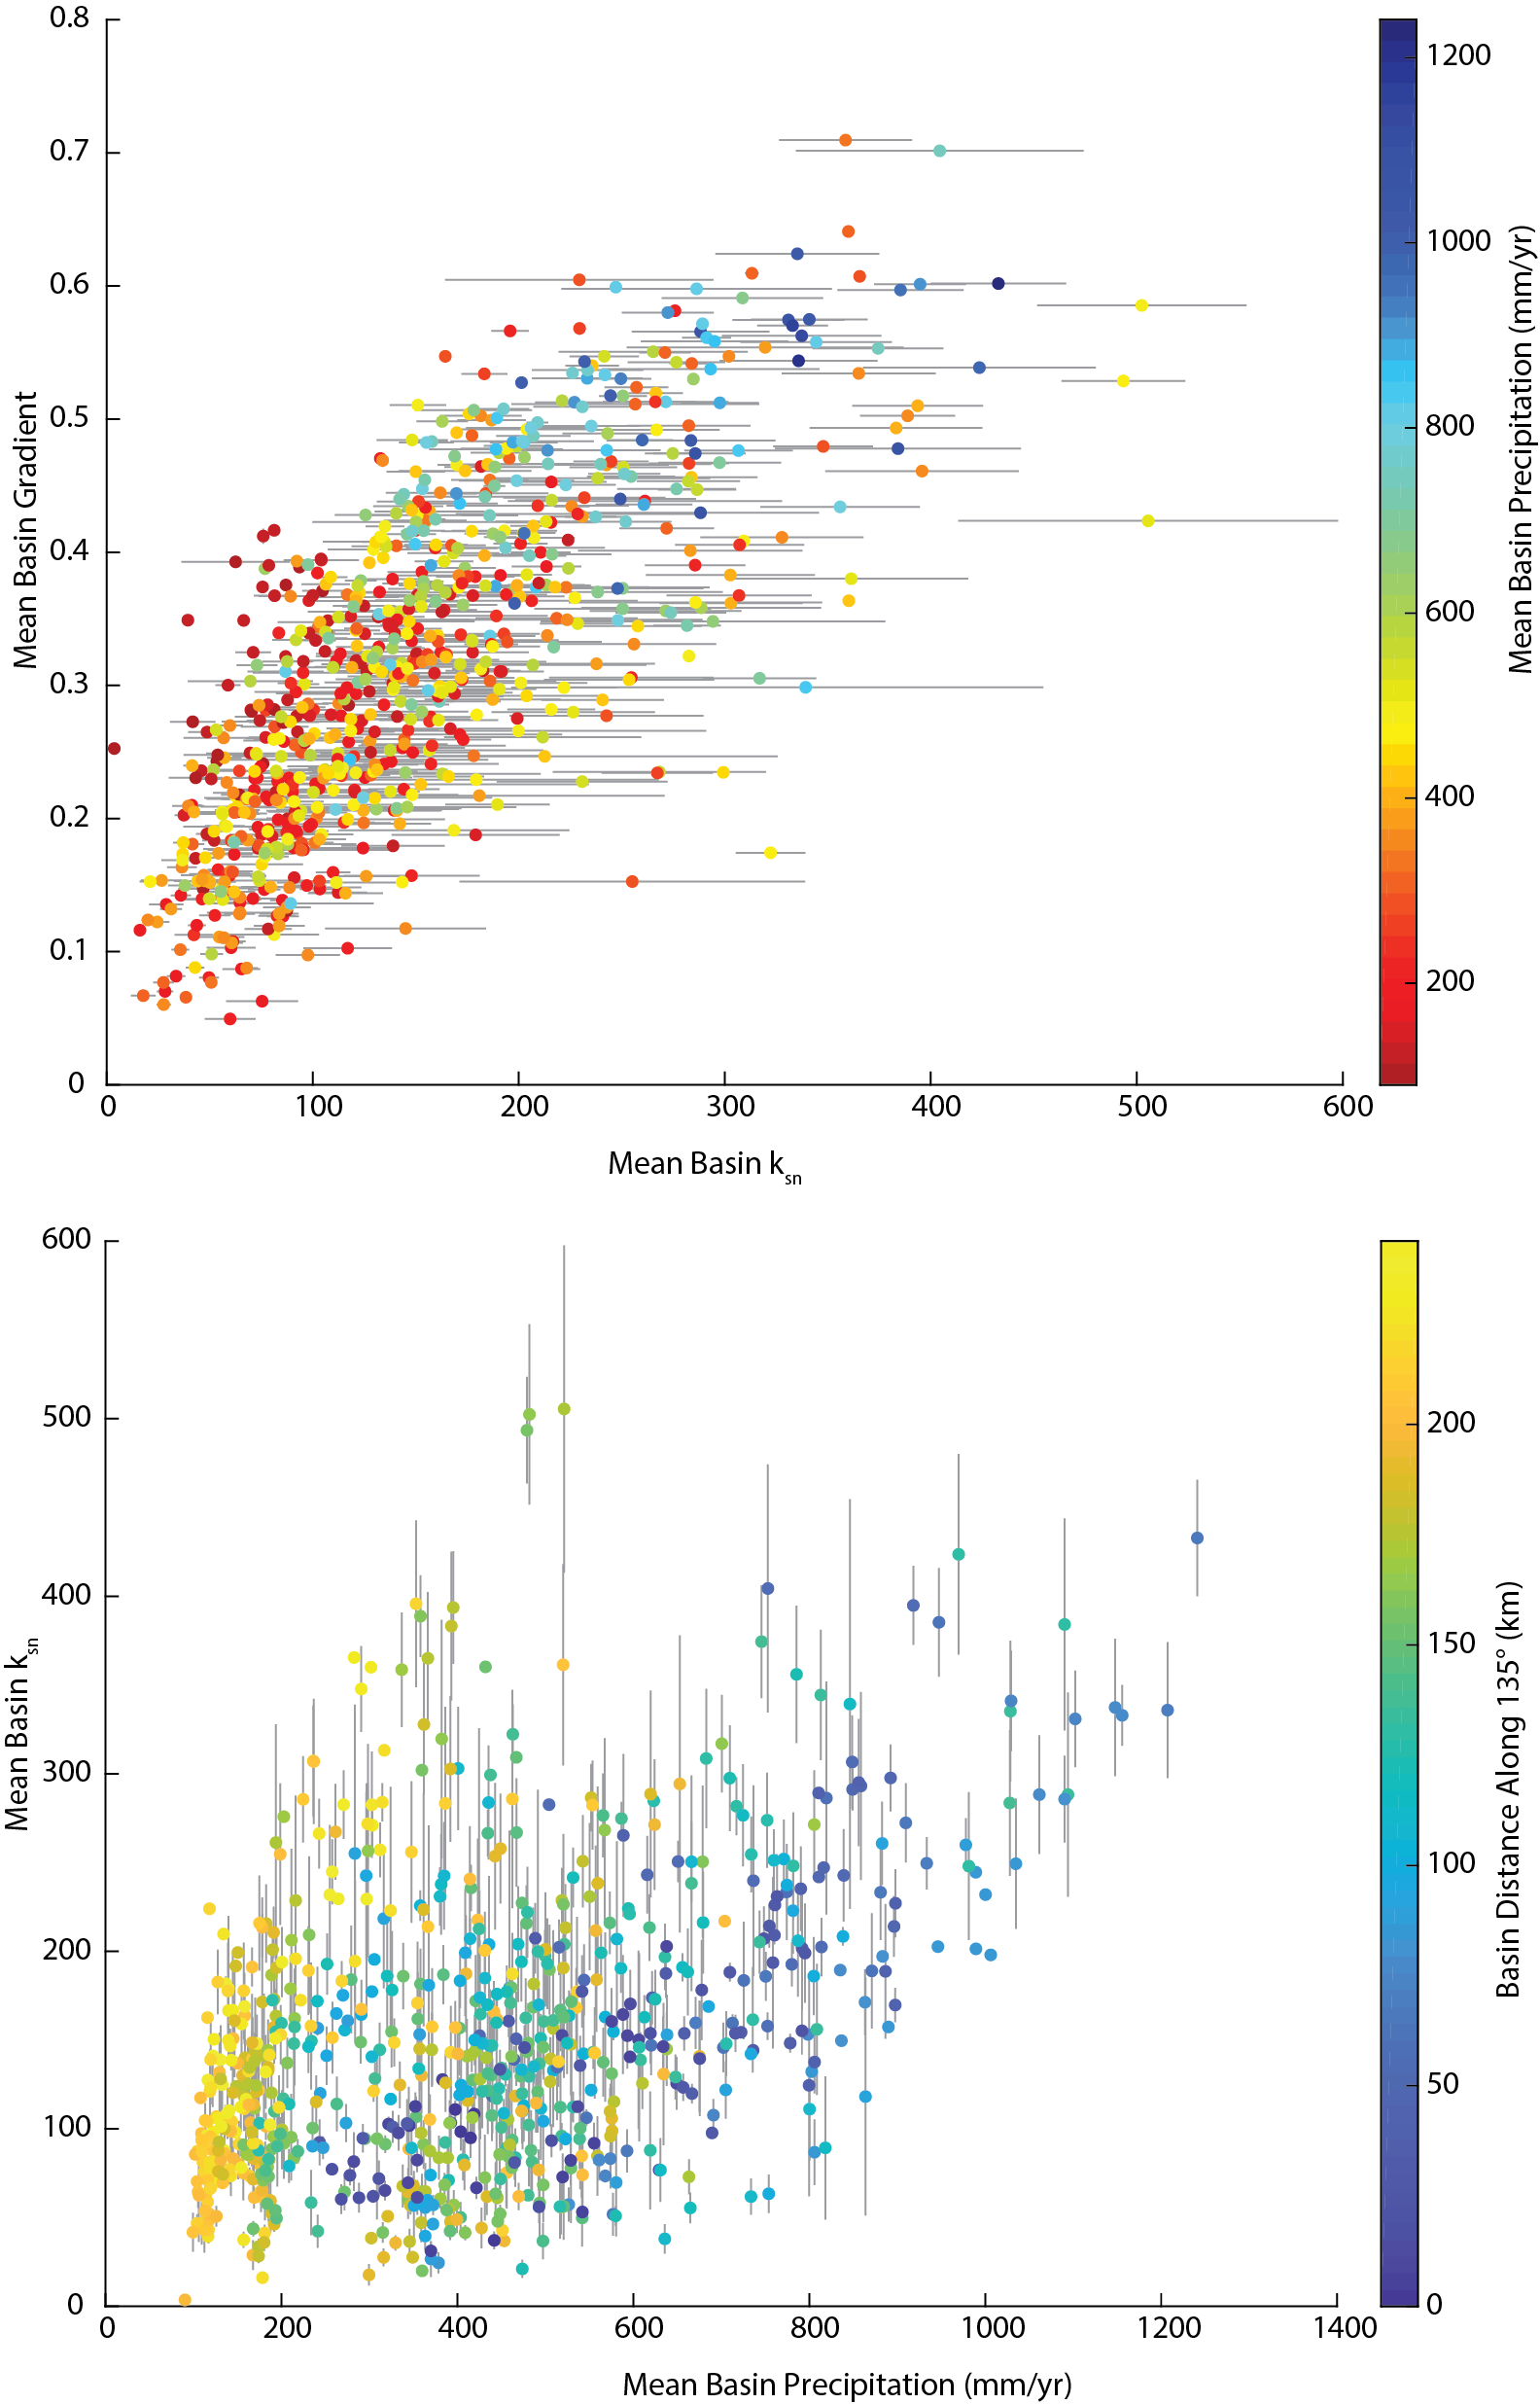
\includegraphics[width=10cm]{PNGs/BasinStats.png}
	\caption{Selected outputs of \nameref{sec:BSPlots} showing some options for plots using the \textit{'color\_by'} optional parameter. Data is from the Southern California sample dataset using the basins $>$ 100 km\textsuperscript{2}  filtered by trunk confluences $>$ 5 km\textsuperscript{2}.}
	\label{fig:BsnSts}
\end{figure}

\subsubsection{Mean Gradient vs Mean \textit{k\textsubscript{sn}} - \textit{'grd\_ksn'}} \label{sec:grdksn}
\paragraph{}Both mean hillslope gradient and mean \textit{k\textsubscript{sn}} have previously been shown to correlate to mean erosion rate  and reflect the morphologic response of hillslope and fluvial domains to the erosion rate, respectively. Thus, in the absence of quantitative erosion rate data for a portions of basins, there can be utility in examining the relationship between mean hillslope gradient and mean \textit{k\textsubscript{sn}}, see \href{https://www.sciencedirect.com/science/article/pii/S0012821X16303004}{Forte et al., 2016} for a full discussion of the nuances of interpreting these relationships. The \textit{'grd\_ksn'} plot option will plot these two quantities against each other (Figure \ref{fig:GrdKsnComp}). 

\begin{figure}[H]
	\centering
	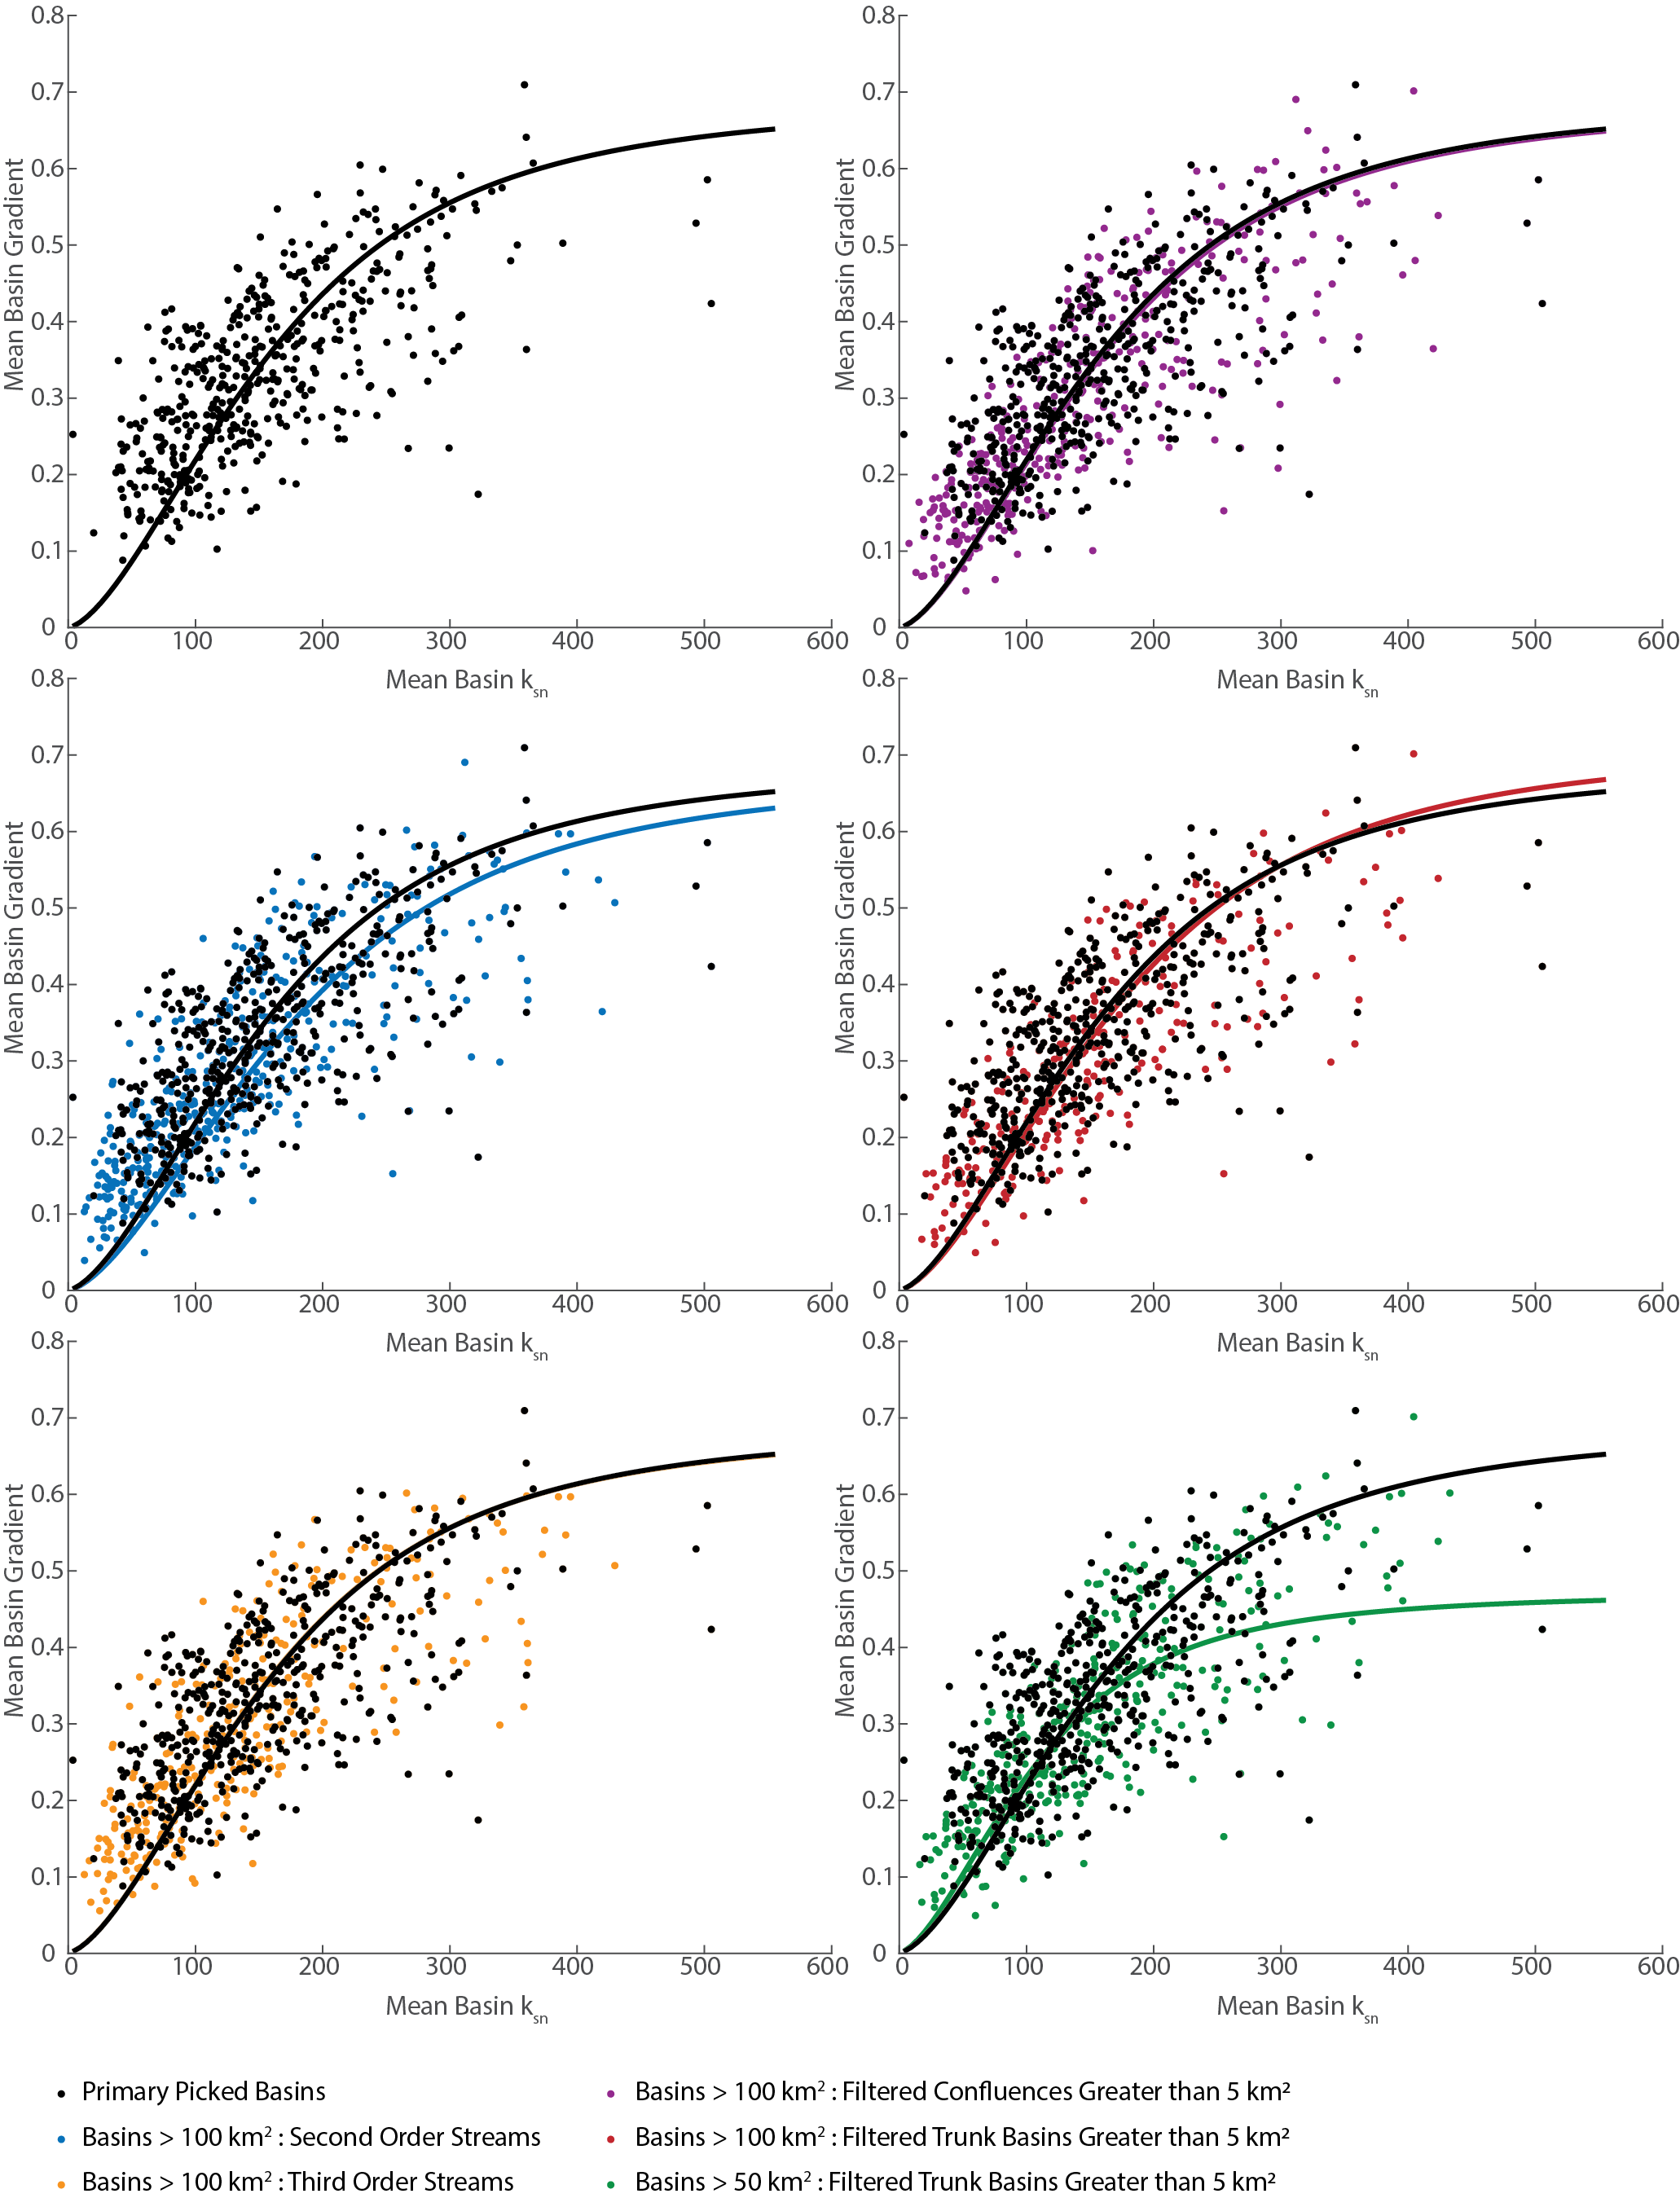
\includegraphics[width=13cm]{PNGs/grd_ksn_basinCompare.png}
	\caption{Comparisons of mean \textit{k\textsubscript{sn}} vs mean basin gradient and associated fits  for a variety of sub-basin division schemes using \nameref{sec:SbDvdBsn} using the \textit{'grd\_ksn'} plot from \nameref{sec:BSPlots}. See Figure \ref{fig:BasinsComp} for a map view of these different basin division schemes.}
	\label{fig:GrdKsnComp}
\end{figure}


\paragraph{}Via the optional \textit{'fit\_grd\_ksn'} parameter, you can also use the relationship between mean hillslope gradient and mean \textit{k\textsubscript{sn}} to estimate some morphometric parameters for the populations of basins, specifically the erosional efficiency, hillslope diffusivity, and limiting gradient. In detail, the analysis relies on the idea that the morphology of both the hillslope and fluvial portions of a landscape vary as a function of erosion rate. We can use these relationships with erosion rates, even if the erosion rates are unknown, to estimate these parameters. For the fluvial portion of the landscape, we use:

\begin{equation}
E=K(k_{sn})^{n}
\end{equation}

\noindent
where $E$ is mean erosion rate, $K$ is fluvial erosional efficiency, $k_{sn}$ is basin mean normalized channel steepness, and $n$ is the slope exponent from the stream power law \citep[e.g.,][]{Snyder2003,Ouimet2009}. For the hillslope portion of the basin, we use the combination of two equations from \cite{Roering2007}, first an equation for variation of hillslope elevation $z$ as a function of distance $x$:

\begin{equation}
z(x) = \frac{-{S_{c}}^{2}}{2\beta E}  \bigg[ \sqrt{D^{2} + (2\beta Ex / S_{c})^{2}} -D\ln\bigg( \frac{ \sqrt{D^{2} + (2\beta Ex / S_{c})^{2}} + D}{2\beta E/S_{c}} \bigg)   \bigg]
\end{equation}

\noindent
where $S_{c}$ is a limiting hillslope gradient where sediment flux becomes infinite, $D$ is a diffusivity coefficient, $\beta = (\rho_{r}/\rho_{s})$ and $\rho_{r}$ and $\rho_{s}$ are the densities of rock and sediment and $\beta$ is set to 2. This equation is in turn used to determine a mean hillslope gradient, $S_{avg}$, (as a function of erosion rate):

\begin{equation}
S_{avg}=\frac{z(0)-z(L_{H})}{L_{H}}
\end{equation}

\noindent where $L_{H}$ is a characteristic hillslope length, which is found by numerically solving the following expression:

\begin{equation}
\bigg(  \frac{E}{2K{L_{H}}^{2}}  \bigg)^{\frac{1}{n}} = \frac{D{S_{c}}^{2}}{\beta E |L_{H}|} \Bigg( \sqrt{1 + \bigg( \frac{\beta E L_{H}}{DS_{c}} \bigg)^{2} } - 1 \Bigg)
\end{equation}

\noindent which is effectively finding the distance from the divide where the slope of the hillslope portion and fluvial portions of the landscape are equal and that the contributions from erosion of the hillslope and fluvial portions of the landscape are also equal \citep[e.g.,][]{Howard1997,Perron2008}. The fits are done via a constrained minimization of least absolute deviation on the above set of equations, and to successfully run the fits, you need access to the Optimization Toolbox in Matlab. The fits are sensitive to the choice of initial parameters, which you can control with the optional \textit{'start\_diffusivity'}, \textit{'start\_erodibility'}, and \textit{'start\_threshold\_gradient'} parameters, which are starting values for $D$, $K$, and $S_{c}$ respectively. Also important is the optional \textit{'n\_val'} parameter (i.e. $n$) which is not a free parameter  (i.e. you must provide a value for \textit{'n\_val'} are use the default value of 2) in the fits, but will control the shape of the fluvial portion of the relationship. We refer readers who are more interested in the nuances of this fit and the (large) assumptions that go into it to \href{https://www.sciencedirect.com/science/article/pii/S0012821X16303004}{Forte et al., 2016} and references therein. Exploring the shape of this relationship (and thus the estimated values for the parameters that control it) also highlights that choosing different methods of subdivision of basins using \nameref{sec:SbDvdBsn} can produce statistically different populations of basins (e.g. Figure \ref{fig:GrdKsnComp}). It should be emphasized that the values for the limiting gradient, fluvial erodibility, and hillslope diffusivity extracted from this fit should be considered with some level of skepticism. If quantitative erosion rates are available for a region of interest, using these erosion rates to estimate the referenced parameters will always yield a more reliable result. The purpose of using the relationships here is mostly for relative comparison between basins within a study region.

\subsubsection{Mean Gradient vs Mean Relief - \textit{'grd\_rlf'}} \label{sec:grdrlf}
\paragraph{}You can also plot mean gradient vs. mean local relief via the \textit{'grd\_rlf'} plot option. This should be similar to the result of \nameref{sec:grdksn} plot as mean local relief and mean \textit{k\textsubscript{sn}} are typically linearly related (depending on the relief radius). You can test the nature of the relationship between mean local relief and mean \textit{k\textsubscript{sn}} with the \nameref{sec:rlfksn} plot option. The \textit{'grd\_rlf'} plot will use the relief radius specified with the optional \textit{'rlf\_radius'} parameter. If this specifies a relief radius that you did not calculate when running \nameref{sec:PrcRvBsn}, this will result in an error.

\subsubsection{Mean Relief vs Mean \textit{k\textsubscript{sn}} - \textit{'rlf\_ksn'}} \label{sec:rlfksn}
\paragraph{}Depending on the relief radius, the relationship between mean local relief and mean \textit{k\textsubscript{sn}} should be linear, but you can quickly test this with the \textit{'rlf\_ksn'} option which will plot these two quantities against each other. The \textit{'rlf\_ksn'} plot will use the relief radius specified with the optional \textit{'rlf\_radius'} parameter. If this specifies a relief radius that you did not calculate when running \nameref{sec:PrcRvBsn}, this will result in an error. 

\subsubsection{Comparing Filtered and Non-Filtered Means - \textit{'compare\_filtered'}} \label{sec:compfilt}

\paragraph{}If you calculated filtered means when running \nameref{sec:CompStats}, the \textit{'compare\_filtered'} option will plot the filtered means against the unfiltered means and visually highlight basins that imply higher filtered values compared to non-filtered with red dots and basins that imply lower filtered values compared to non-filtered with blue dots (e.g. Figure \ref{fig:FiltBsnComp}). This plot option will produce an individual plot for any quantity for which a mean and a filtered mean was calculated (obviously, if filtered means were not calculated, this option will produce an error). In the example, we present examples of mean \textit{k\textsubscript{sn}} and mean gradient in the case of a filter excluding quaternary units from the means and an inclusive filter calculating means from granites, metamorphic rocks, and other 'basement' rocks (Figure \ref{fig:FiltBsnComp}). This allows you to assess relatively quickly that removing areas covered by quaternary units shifts means toward higher values, where as only calculating means based on 'hard rocks' also shifts many basins to higher means values, but not in all cases. This will of course depend on the nature of the filter and like the majority of the plots, this is designed as a data exploration tool to determine what aspects warrant deeper analysis.

\begin{figure}[H]
	\centering
	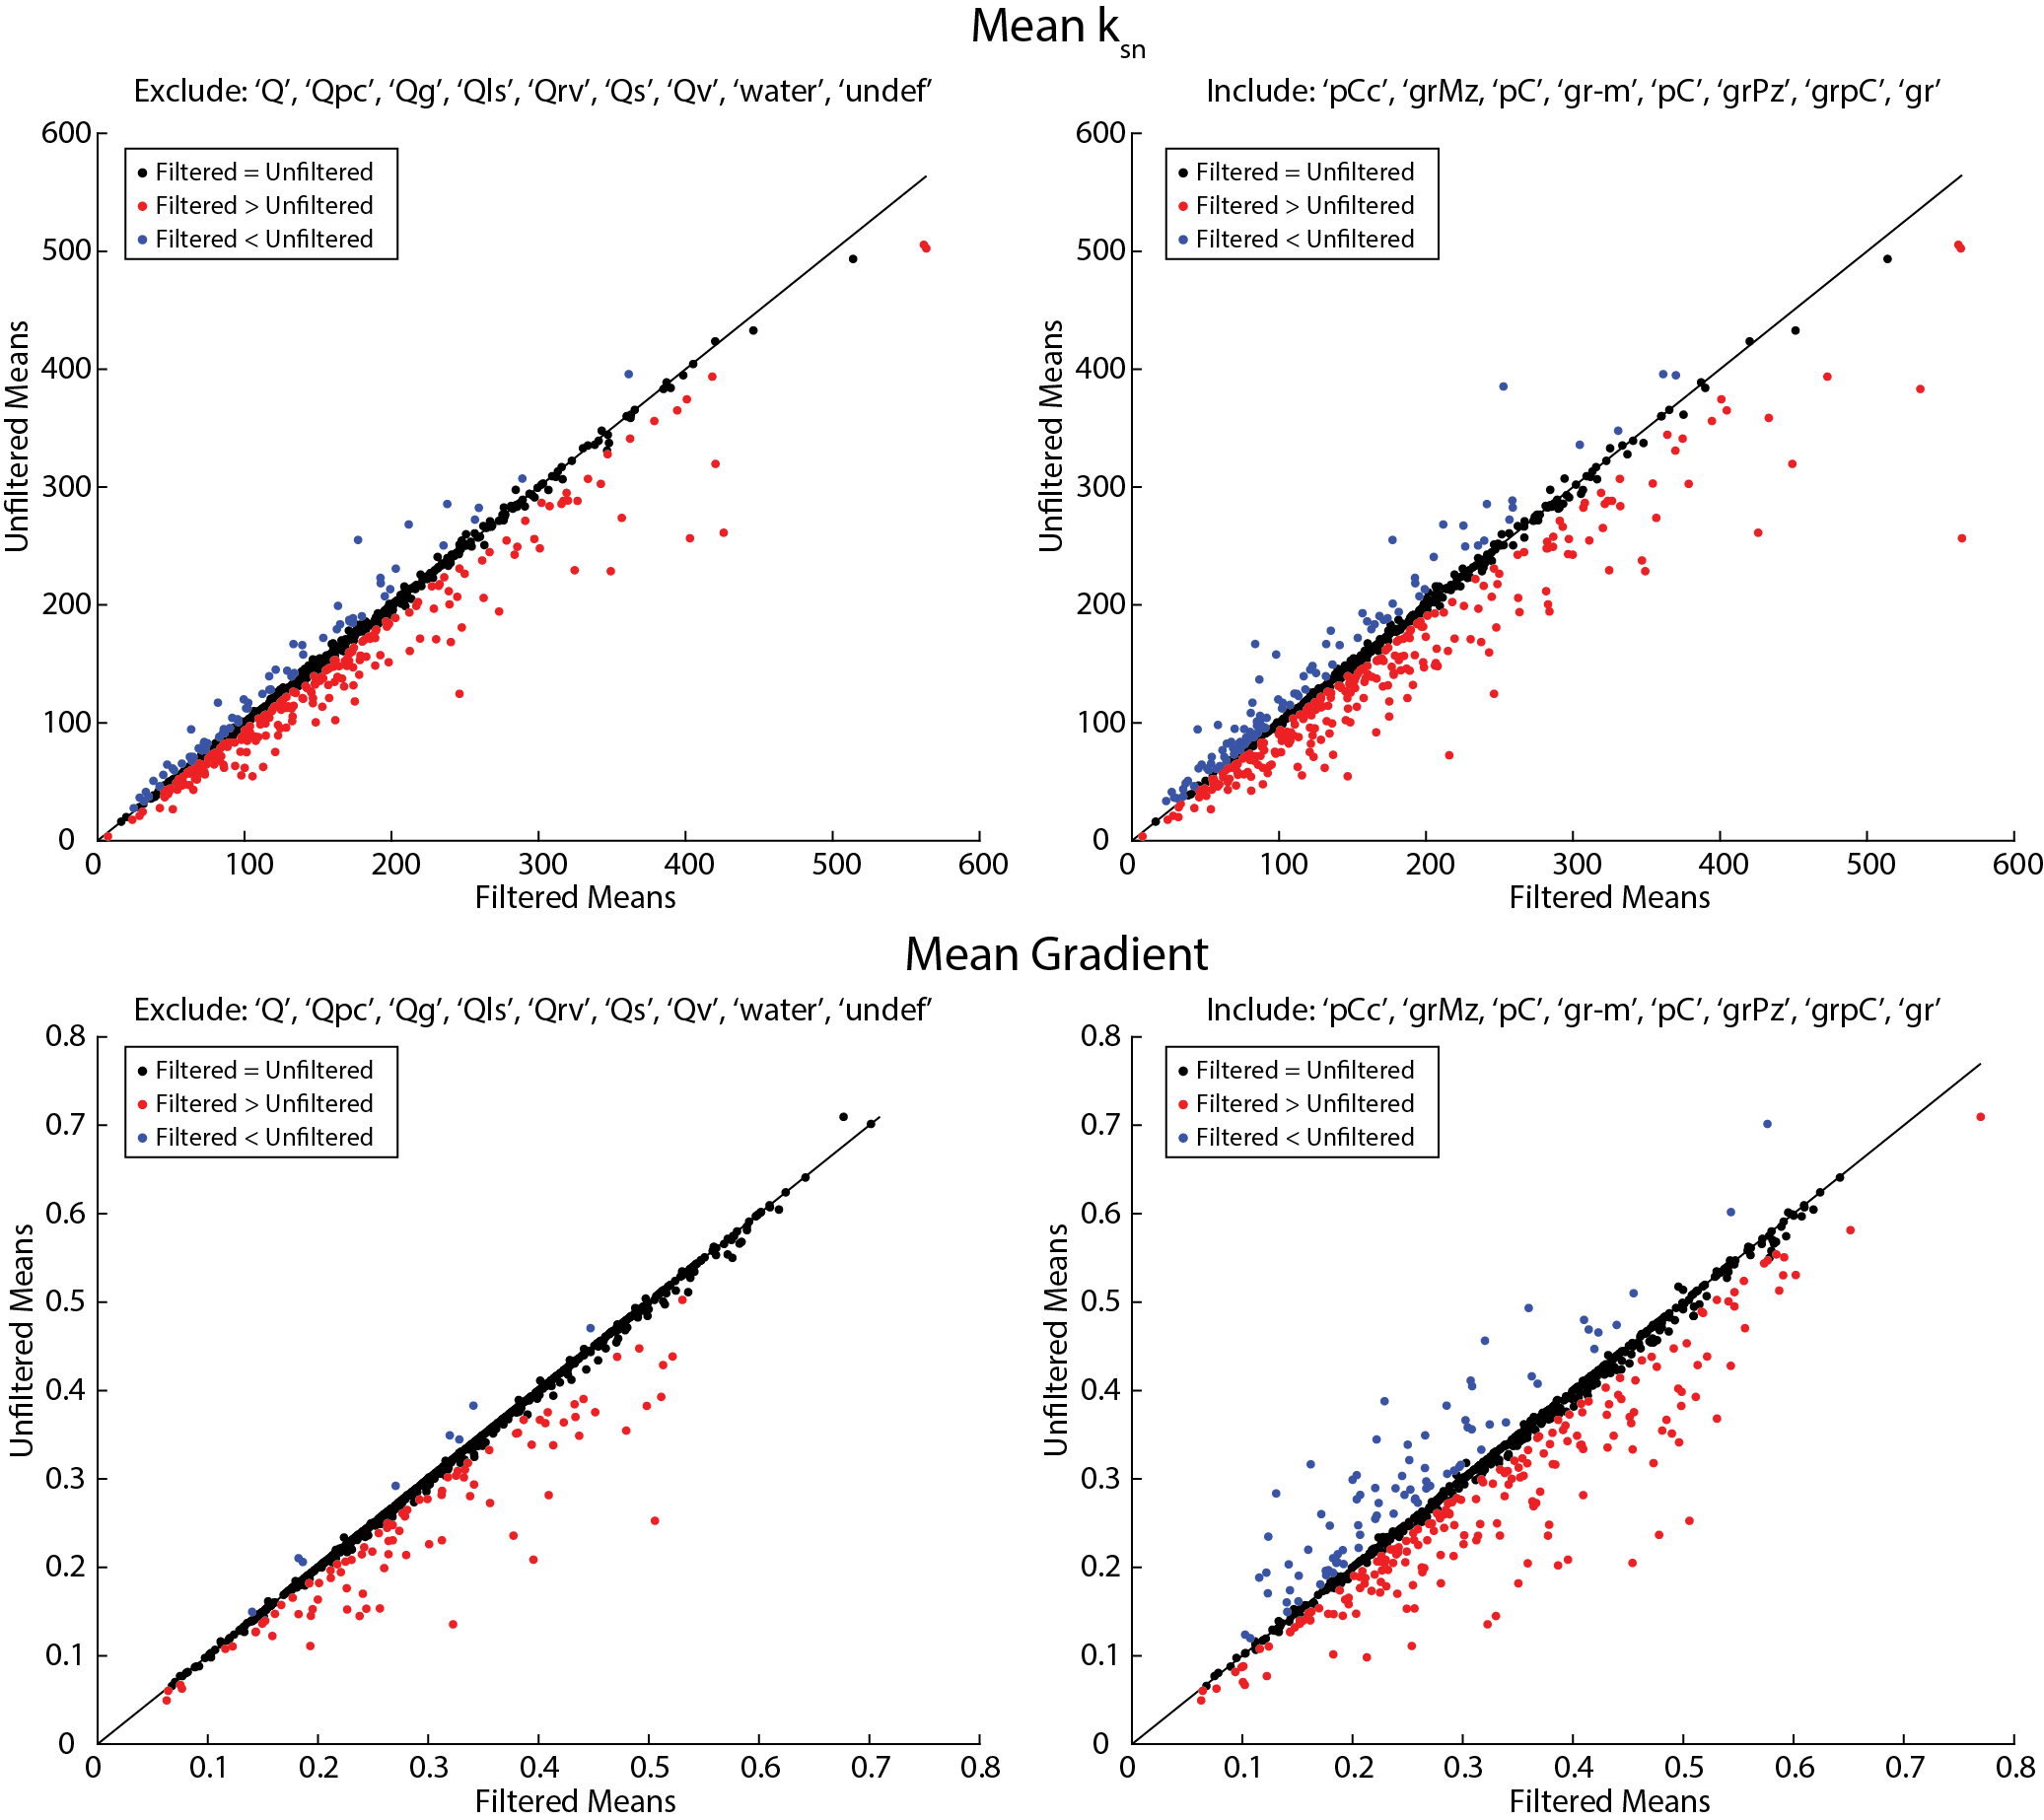
\includegraphics[width=16.5cm]{PNGs/Filtered_Basin_Comparison.png}
	\caption{Selected outputs of \textit{'compare\_filtered'} plot from \nameref{sec:BSPlots} comparing results of an excluding quaternary, water, and undefined areas vs including basement rocks. Data is from the Southern California sample dataset using the basins $>$ 100 km\textsuperscript{2}  filtered by trunk confluences $>$ 5 km\textsuperscript{2}.}
	\label{fig:FiltBsnComp}
\end{figure}

\subsubsection{Histograms of Category Means - \textit{'category\_mean\_hist'}} \label{sec:cathist}
\paragraph{}If you calculate means by categories when running \nameref{sec:CompStats}, you can use the \textit{'category\_mean\_hist'} option to plot histograms of the means across all basins within given categories for a statistic of interest. Using this option requires providing an argument to the optional \textit{'cat\_mean1'} parameter to specify which statistic (e.g. mean \textit{k\textsubscript{sn}}) for which you wish to produce histograms.

\subsubsection{Comparisons of Category Means - \textit{'category\_mean\_compare'}} \label{sec:catcomp}
\paragraph{}If you calculate means by categories when running \nameref{sec:CompStats}, you can use the \textit{'category\_mean\_compare'} option to compare two statistics of interest within the categories (e.g. plots of mean basin \textit{k\textsubscript{sn}} vs mean gradient as a function of rock type). Using this option requires providing arguments to the optional \textit{'cat\_mean1'}  and \textit{cat\_mean2'} parameters to specify which statistics you want to compare.

\begin{figure}[H]
	\centering
	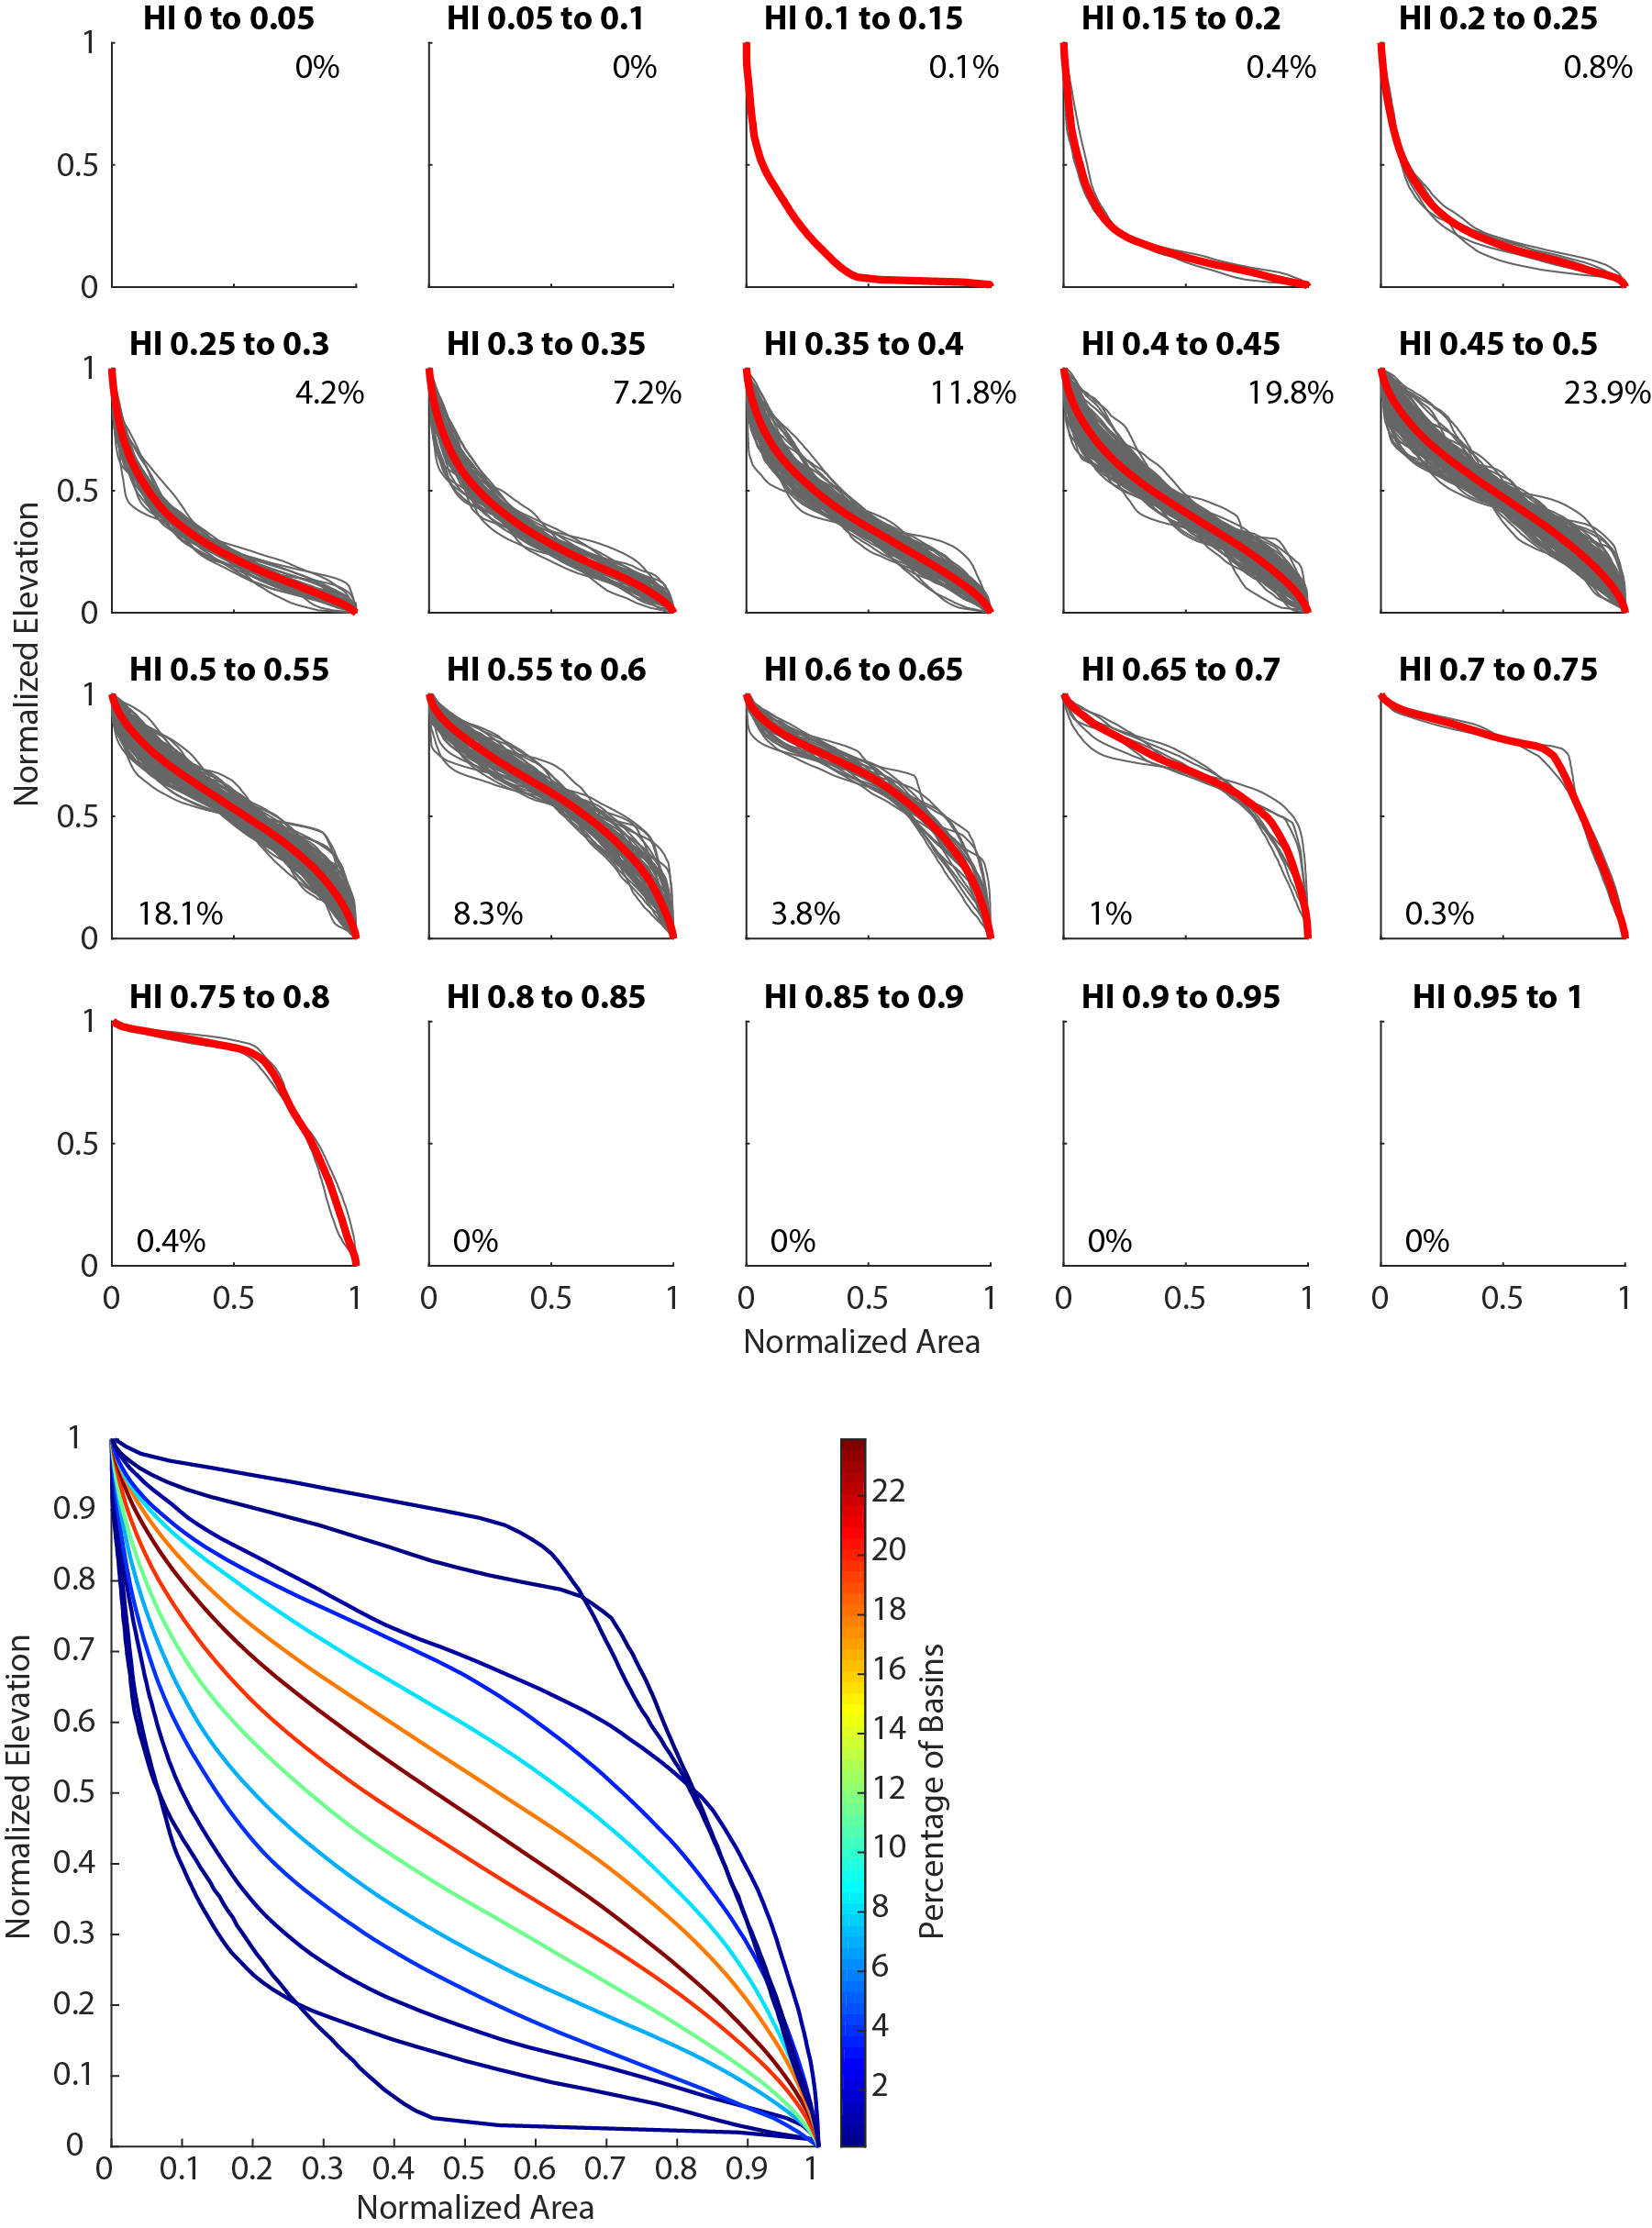
\includegraphics[width=12cm]{PNGs/BasinHypsometry.png}
	\caption{Selected output of \textit{'stacked\_hypsometry'} plots from \nameref{sec:BSPlots}. Data is from the Southern California sample dataset using the basins $>$ 100 km\textsuperscript{2}  filtered by trunk confluences $>$ 5 km\textsuperscript{2}.}
	\label{fig:Hyps}
\end{figure}

\subsubsection{Basin Hypsometry - \textit{'stacked\_hypsometry'}} \label{sec:hyps}
\paragraph{}The hypsometry of a basin (e.g. the empirical cumulative distribution of elevations in that basin) and the hypsometric integral (e.g. the area underneath a normalized version of this curve) are classic morphometric parameters, which while simplistic, can still be useful in understanding first order characteristics of a landscape. The \textit{'stacked\_hypsometry'} plot option will produce a series of 5 plots, a subset of which are shown in Figure \ref{fig:Hyps}. This option will plot figures of stacked normalized hypsometries (not included in Figure \ref{fig:Hyps}), a version of the stacked normalized hypsometries displayed as heatmap (not included in Figure \ref{fig:Hyps}), stacked hypsometries with elevations vs percentage area (not included in Figure \ref{fig:Hyps}), a grid of normalized hypsometries with the mean hypsometry binned by the hypsometric integral with the percentages of the basins within that bin (top portion of Figure \ref{fig:Hyps}), and a plot of the mean hypsometries in each hypsometric integral bin and colored by the percentage of basins within that bin (bottom portion of Figure \ref{fig:Hyps}).



\subsubsection{Comparing Distribution of Basin Means vs All Nodes -\textit{'compare\_mean\_and\_dist'}} \label{sec:meanANDdist}
\paragraph{}The \textit{'compare\_mean\_and\_dist'} is designed to explore the distributions of particular statistics within the basins. This option can function in two ways. The first way is by comparing the distribution of a statistic of interest (e.g. mean gradient) across all nodes in all basins compared to the basin means across all basins (Figure \ref{fig:GradDist}). This requires that you specify a statistic to compare using the optional \textit{'statistic\_of\_interest'} parameter.

\begin{figure}[H]
	\centering
	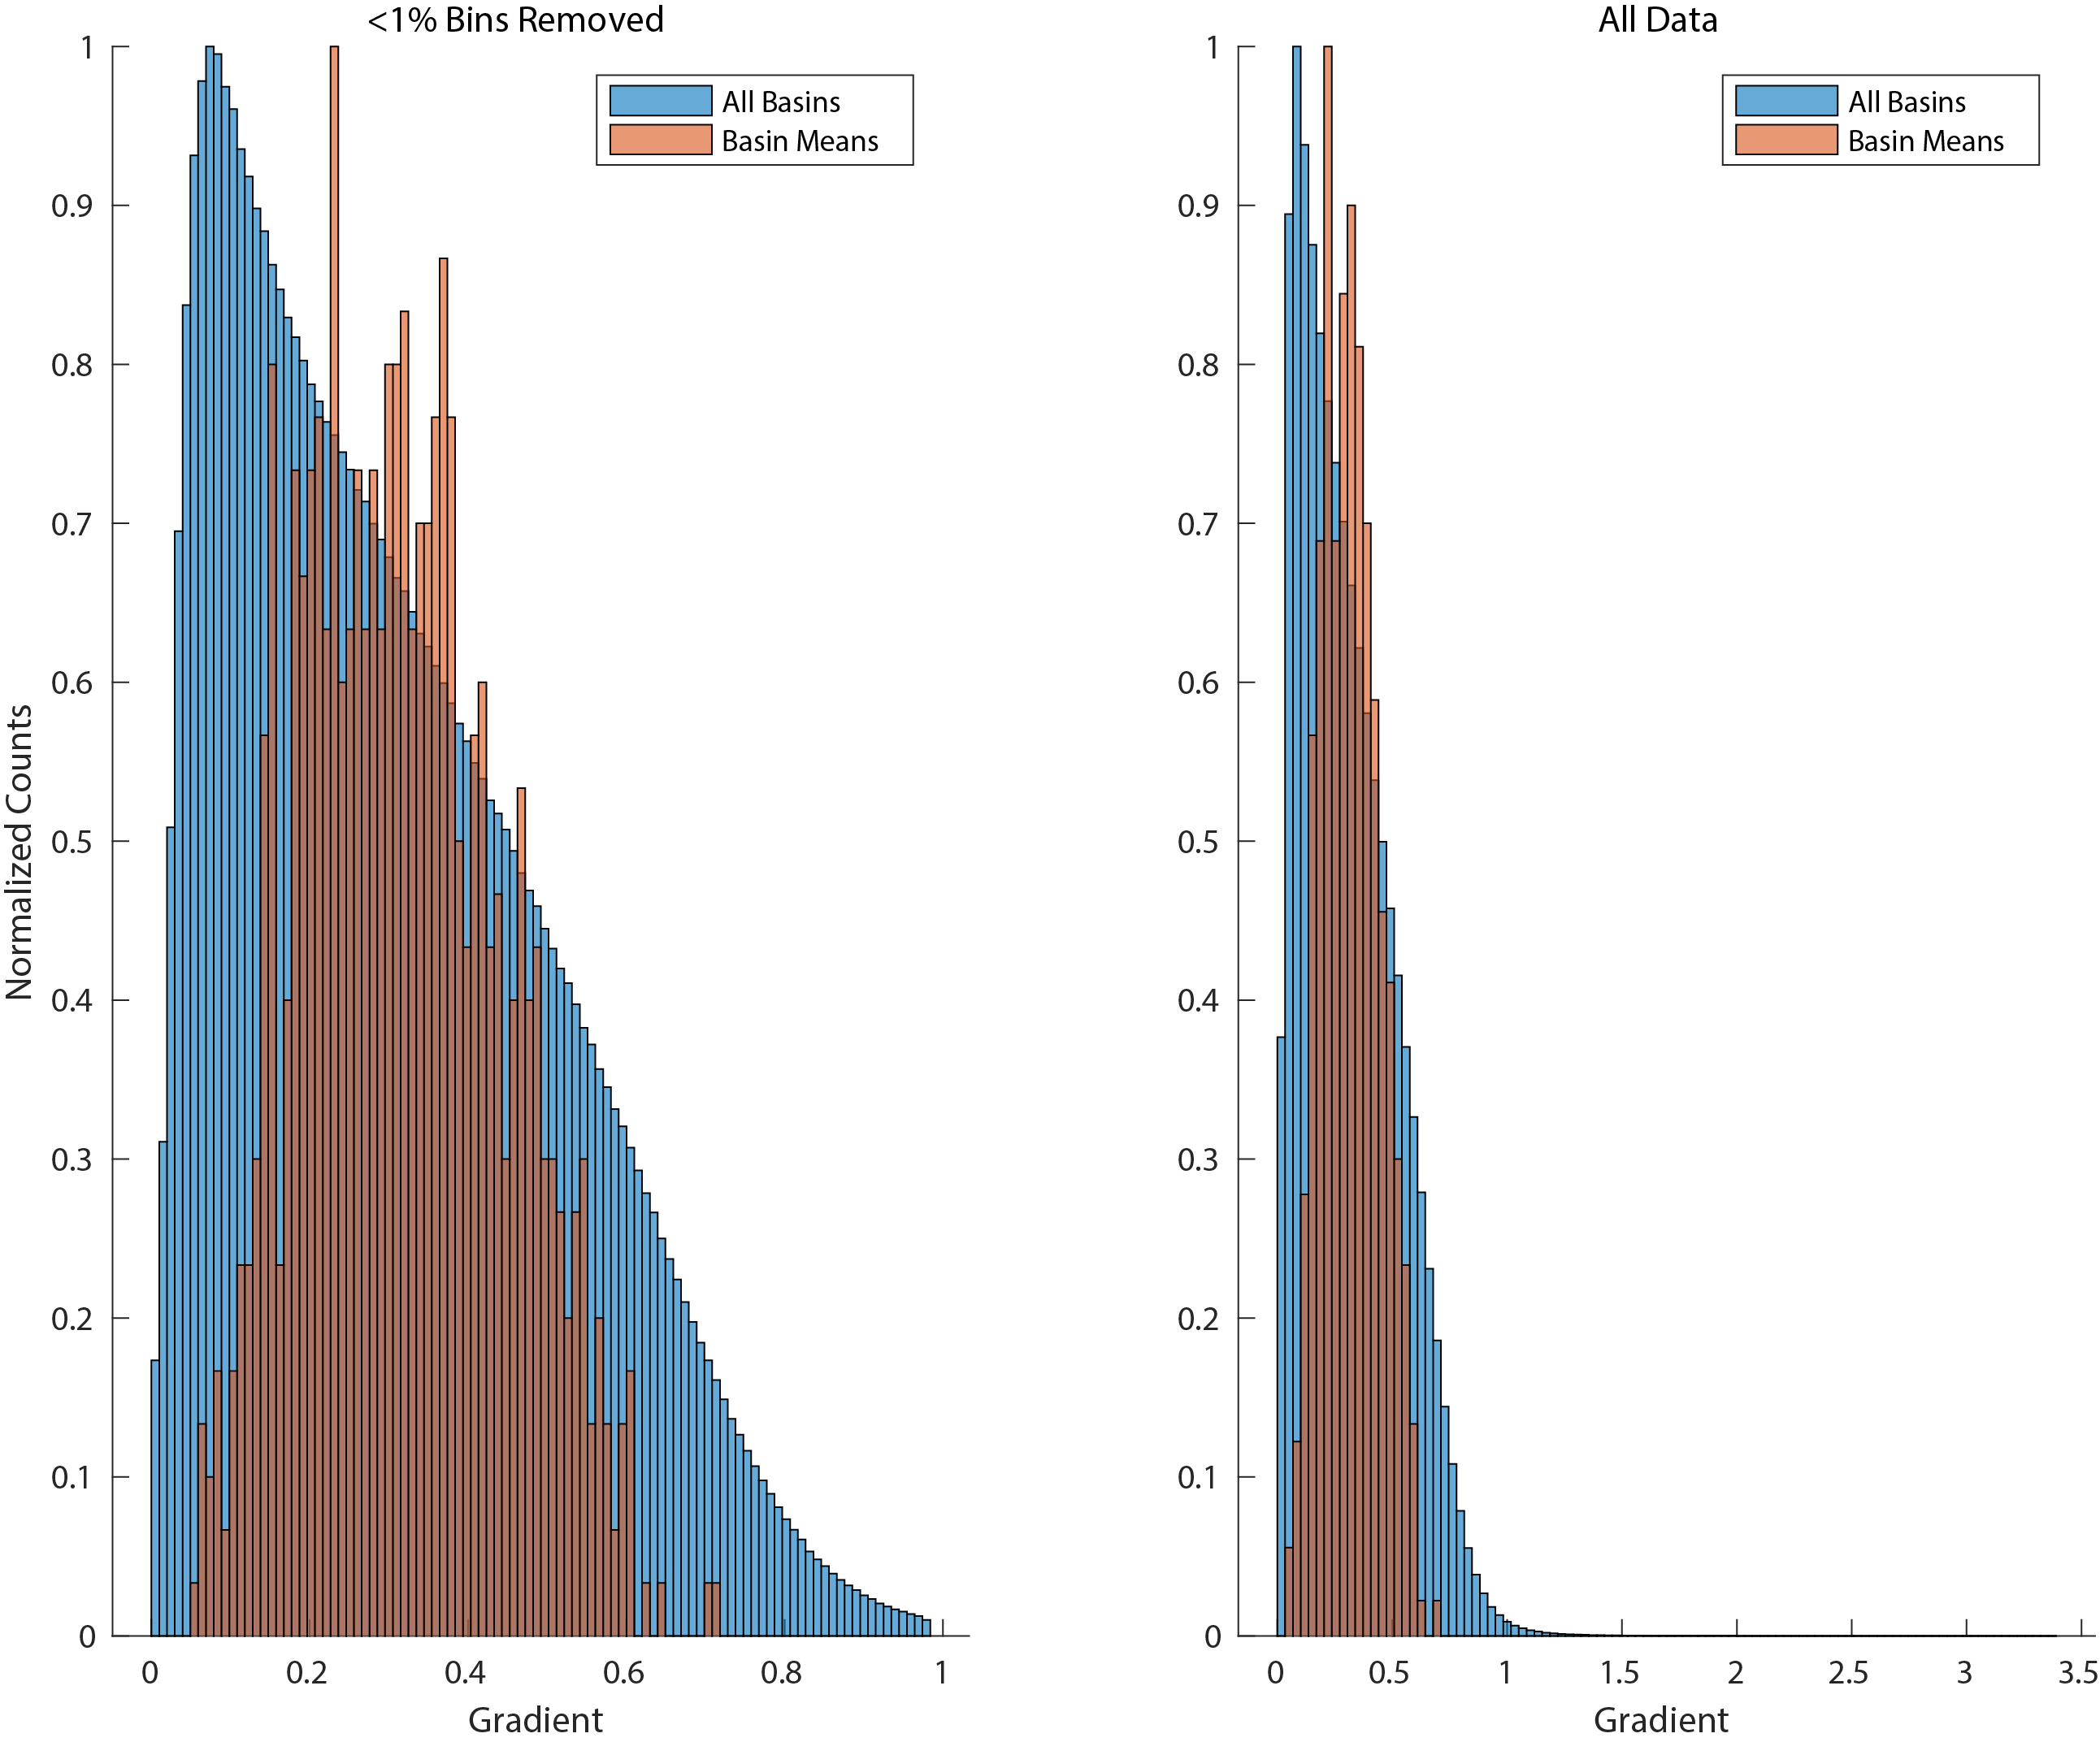
\includegraphics[width=12cm]{PNGs/Gradient_Dist.png}
	\caption{Sample output of \textit{'compare\_mean\_and\_dist'} plot from \nameref{sec:BSPlots} comparing the distribution of gradient across all nodes in all basins (blue) to the distribution of mean gradients across all basins (orange). Data is from the Southern California sample dataset using the basins $>$ 100 km\textsuperscript{2}  filtered by trunk confluences $>$ 5 km\textsuperscript{2}.}
	\label{fig:GradDist}
\end{figure}

\paragraph{}The other way the \textit{'compare\_mean\_and\_dist'}  plot option can be used is to explore the distribution of the statistic of interest of a particular basin compared to the mean value (Figure \ref{fig:KsnDist}). This requires that you specify a statistic to compare using the optional \textit{'statistic\_of\_interest'} parameter and specify a basin of interest by the basin ID number with the \textit{'basin\_num'} parameter.

\begin{figure}[H]
	\centering
	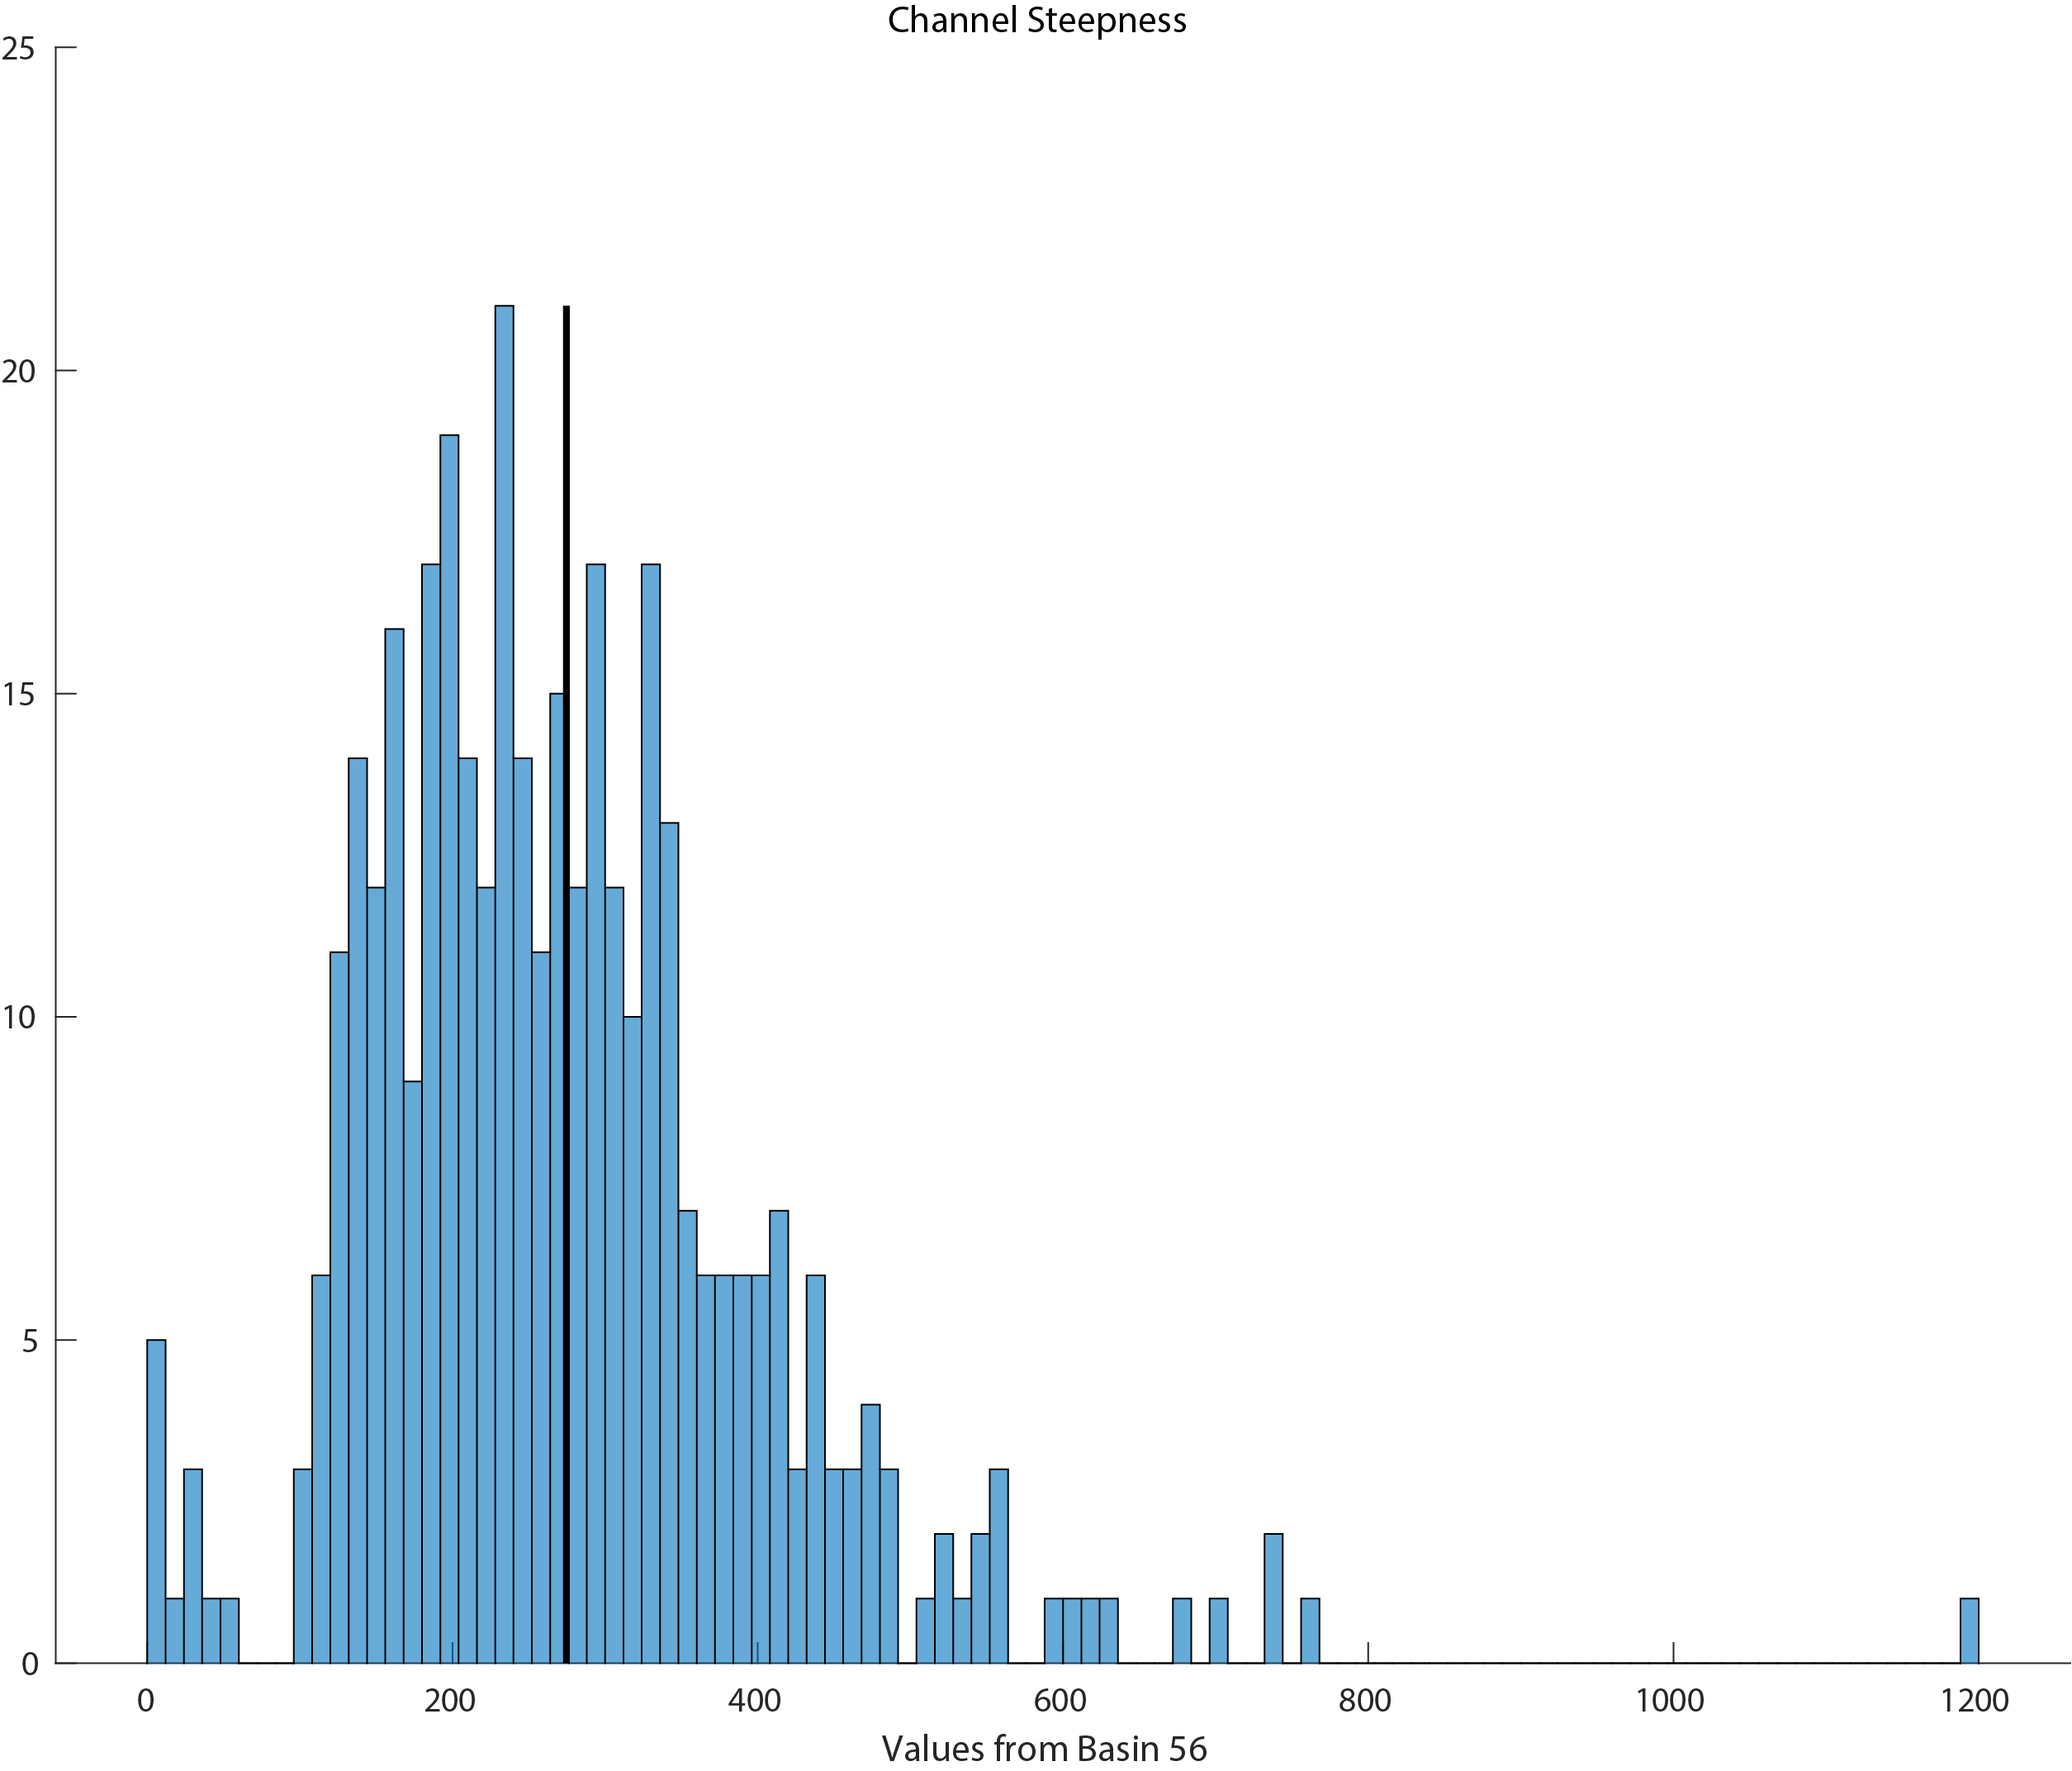
\includegraphics[width=12cm]{PNGs/Basin56_ksn_dist.png}
	\caption{Sample output of \textit{'compare\_mean\_and\_dist'} plot from \nameref{sec:BSPlots} comparing the distribution of \textit{k\textsubscript{sn}} within Basin 56 (in the Southern California dataset) to the mean \textit{k\textsubscript{sn}} within that basin (the thick black line).}
	\label{fig:KsnDist}
\end{figure}


\subsubsection{Grid of Bi-Plots of Means - \textit{'scatterplot\_matrix'}} \label{sec:scattermat}
\paragraph{}The \textit{'scatterplot\_matrix'} plot is designed as a very quick data exploratory tool to look for potential relationships between basin statistics (Figure \ref{fig:ScatterMatrix}). The function will produce a grid of bi-plots comparing the mean values of all metrics for which means were calculated (though this will not include means by categories if calculated). The function also displays a simple second order polynomial fit on the relationship. In positions where values would be compared against each other, the function instead displays a histogram of the distribution of those mean values. For users familiar with R, this is designed to be largely similar to plots produced by the 'lattice' package. 

\paragraph{}As a note, if you calculated filtered means and leave the optional \textit{'use\_filtered'} to false (which is the default) this option will produce a very large matrix as it will include both the regular means and the filtered means. For an input table with filtered means, if you set \textit{'use\_filtered'} to true, the function will use the filtered means to populate the scatterplot matrix. If you want to display the regular means without the filtered means, provide an input table for which you did not calculate filtered means when running \nameref{sec:CompStats}.

\begin{figure}[H]
	\centering
	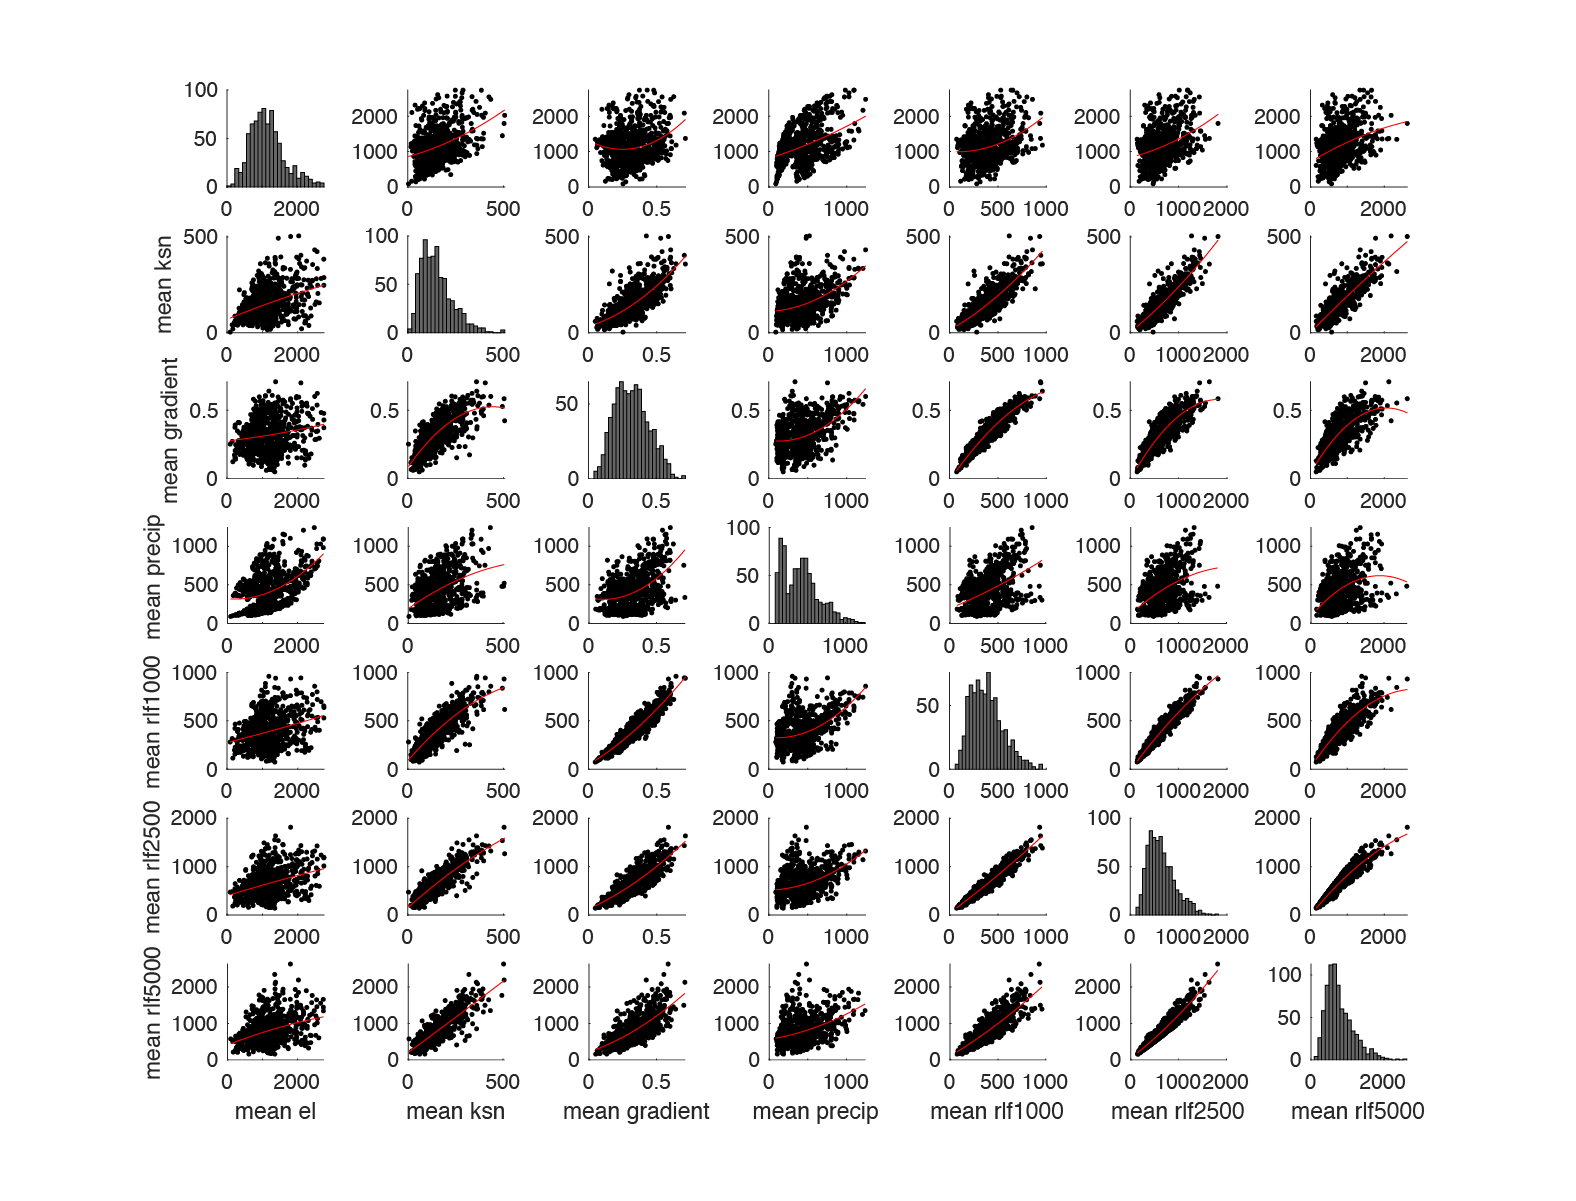
\includegraphics[width=16.5cm]{PNGs/ScatterPlotMatrix.png}
	\caption{Sample output of \textit{'scatterplot\_matrix'} plot from \nameref{sec:BSPlots}. Data is from the Southern California sample dataset using the basins $>$ 100 km\textsuperscript{2}  filtered by trunk confluences $>$ 5 km\textsuperscript{2}.}
	\label{fig:ScatterMatrix}
\end{figure}

\subsubsection{Generic X-Y plot - \textit{'xy'}} \label{sec:xy}
\paragraph{}The final plot option for \nameref{sec:BSPlots} is a generic option to plot any value against any other value. To use this option you must specify the name of the columns to be used as the x and y values via the \textit{'xval'} and \textit{'yval'} parameters. Using conjunction with the \textit{'color\_by'} parameter can quickly produce plots to explore potential relationships within the basin data (e.g. Figure \ref{fig:BsnSts}).


%%%%%%%%
\section{Swath Profiles with Projected Data}
\paragraph{}TopoToolbox includes a robust and simple function to produce swath topographic profiles. We provide two functions in TAK that build and expand upon this functionality and use some swath profiles through our example dataset to illustrate the use of these functions (Figure \ref{fig:XsctMap}).

\begin{figure}[H]
	\centering
	\includegraphics[width=16.5cm]{PNGs/XsctnLocations.png}
	\caption{Location of swaths used to demonstrate uses of \nameref{sec:Swath} and \nameref{sec:CombSwath}.}
	\label{fig:XsctMap}
\end{figure}

\subsection{\textit{MakeTopoSwath}} \label{sec:Swath}
\paragraph{}The \textit{MakeTopoSwath} function is a simple wrapper around the basic functionality of the \textit{SWATHobj} class included as a part of TopoToolbox. The main utility of \textit{MakeTopoSwath} compared to simply using \textit{SWATHobj} natively is more control on the plots produced including different styles of displaying the data, direct control of the vertical exaggeration via the optional \textit{'vex'} parameter, and plotting the location of bends in a swath (Figure \ref{fig:BasicSwath}).

\begin{figure}[H]
	\centering
	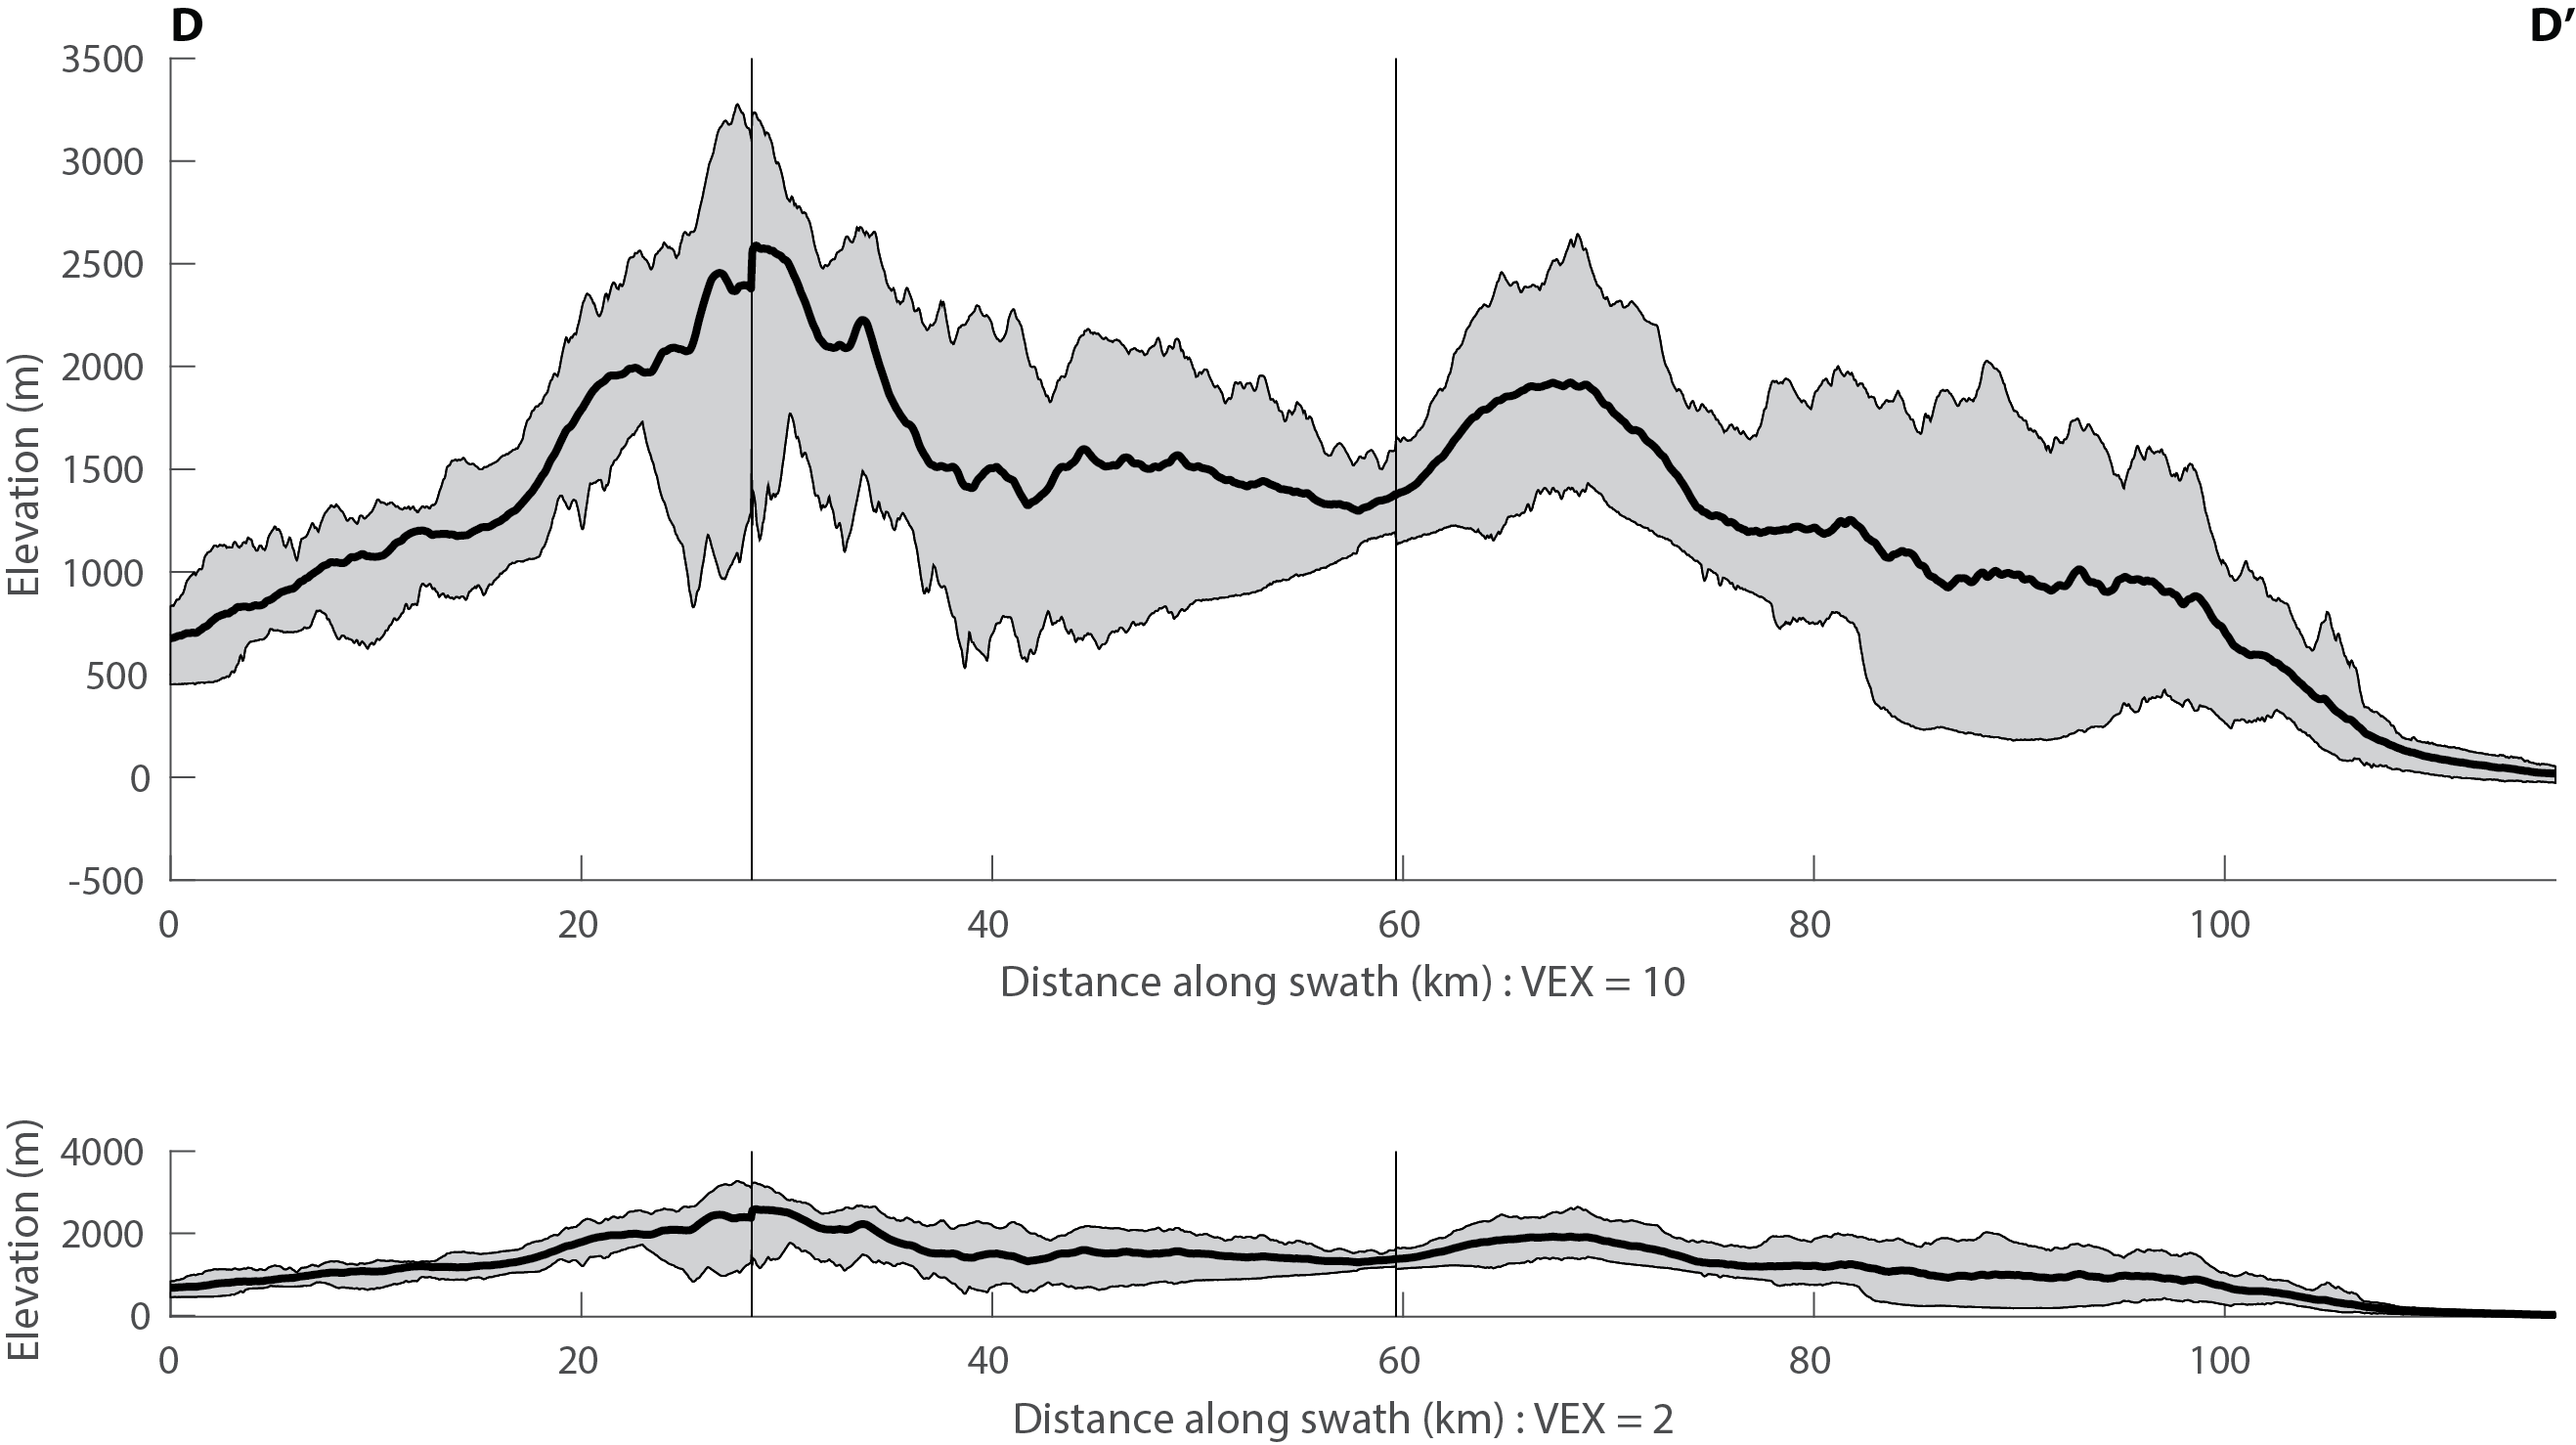
\includegraphics[width=16.5cm]{PNGs/SanJacinto_Swath.png}
	\caption{Basic swaths output from \nameref{sec:Swath} highlighting the function of the \textit{'vex'} parameter to control the vertical exaggeration.}
	\label{fig:BasicSwath}
\end{figure}

\paragraph{}In addition to the basic swath figure, with \textit{MakeTopoSwath}, you can also display the output swath as an array of points (Figure \ref{fig:PointSwath}) by setting \textit{'plot\_as\_points'} to true or a heatmap (Figure \ref{fig:HeatSwath}) by setting \textit{'plot\_as\_heatmap'} to true.

\begin{figure}[H]
	\centering
	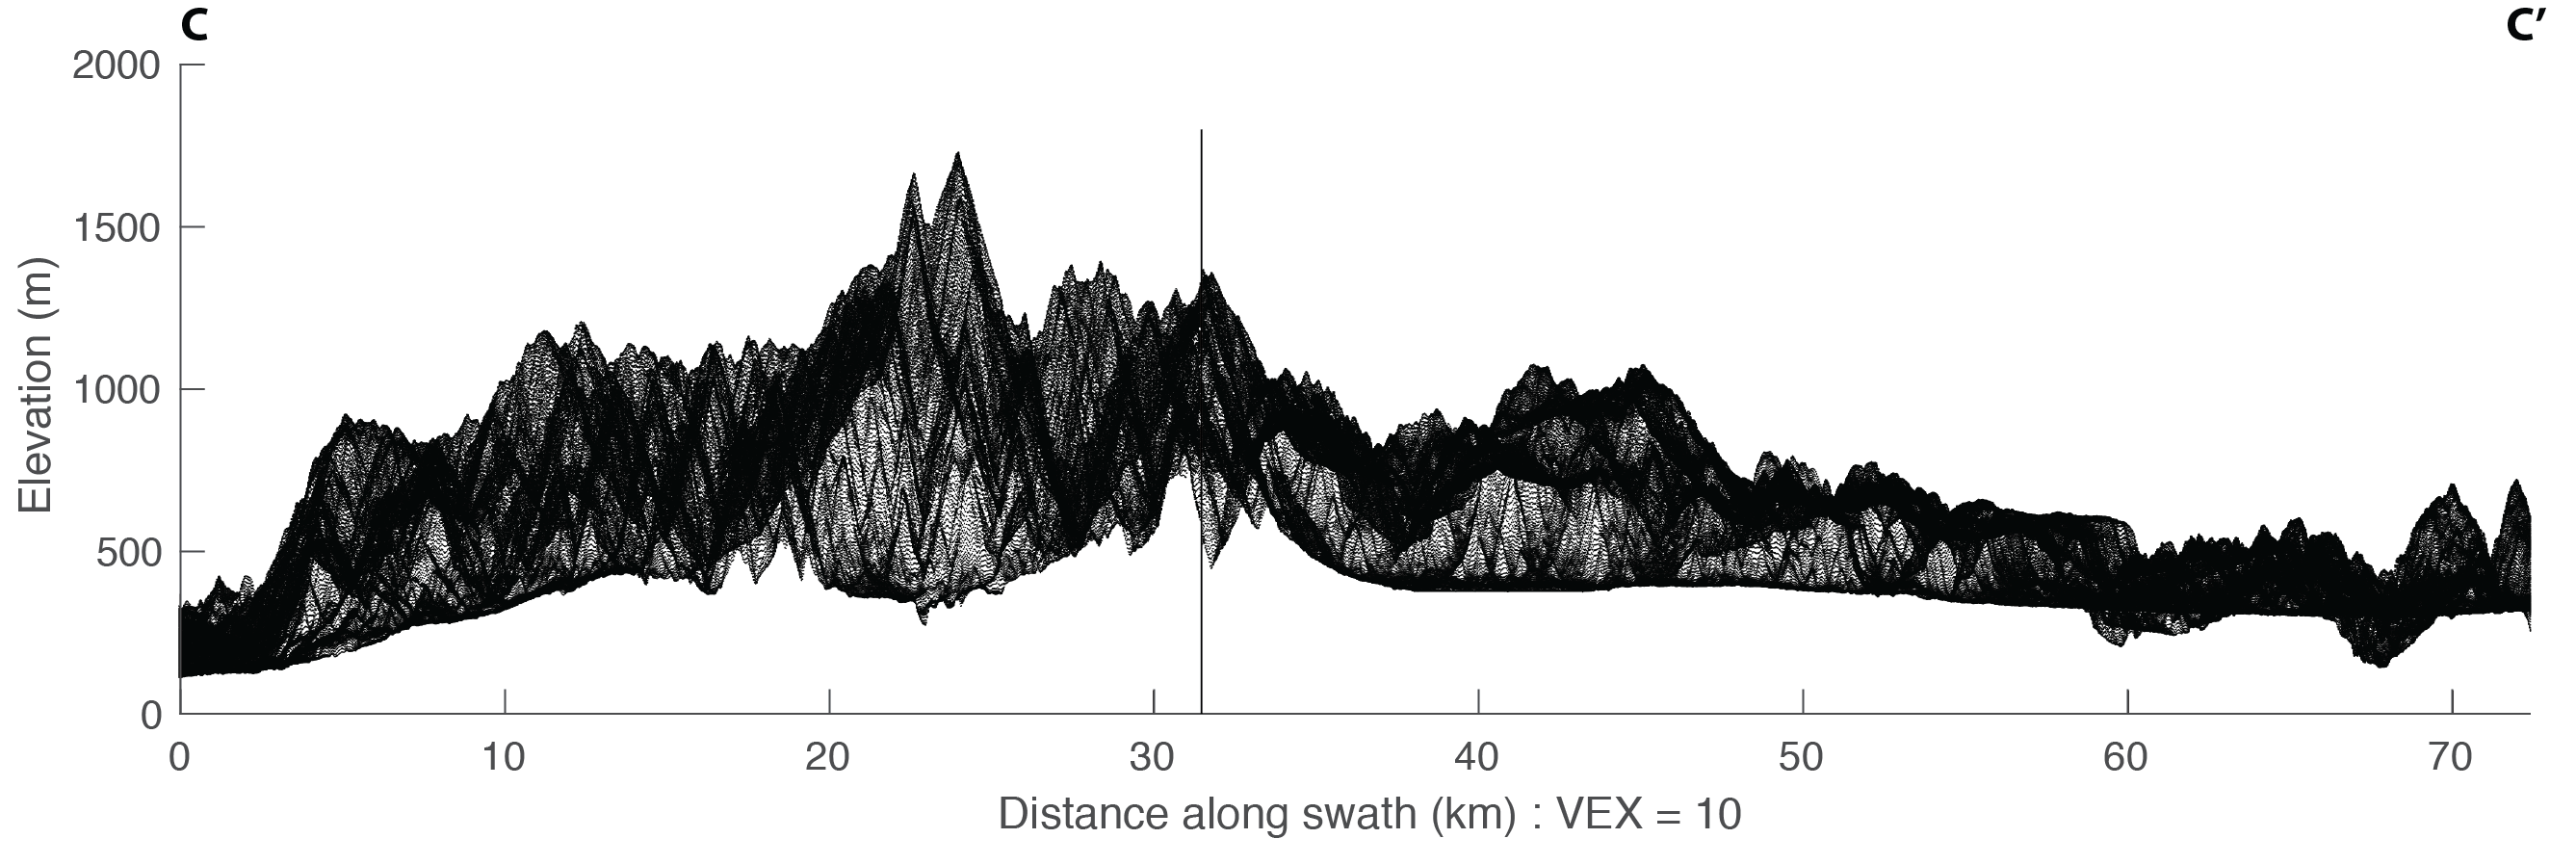
\includegraphics[width=16.5cm]{PNGs/SantAnaSwath_Points.png}
	\caption{Swath output from \nameref{sec:Swath} showing the result of plotting as points.}
	\label{fig:PointSwath}
\end{figure}

\begin{figure}[H]
	\centering
	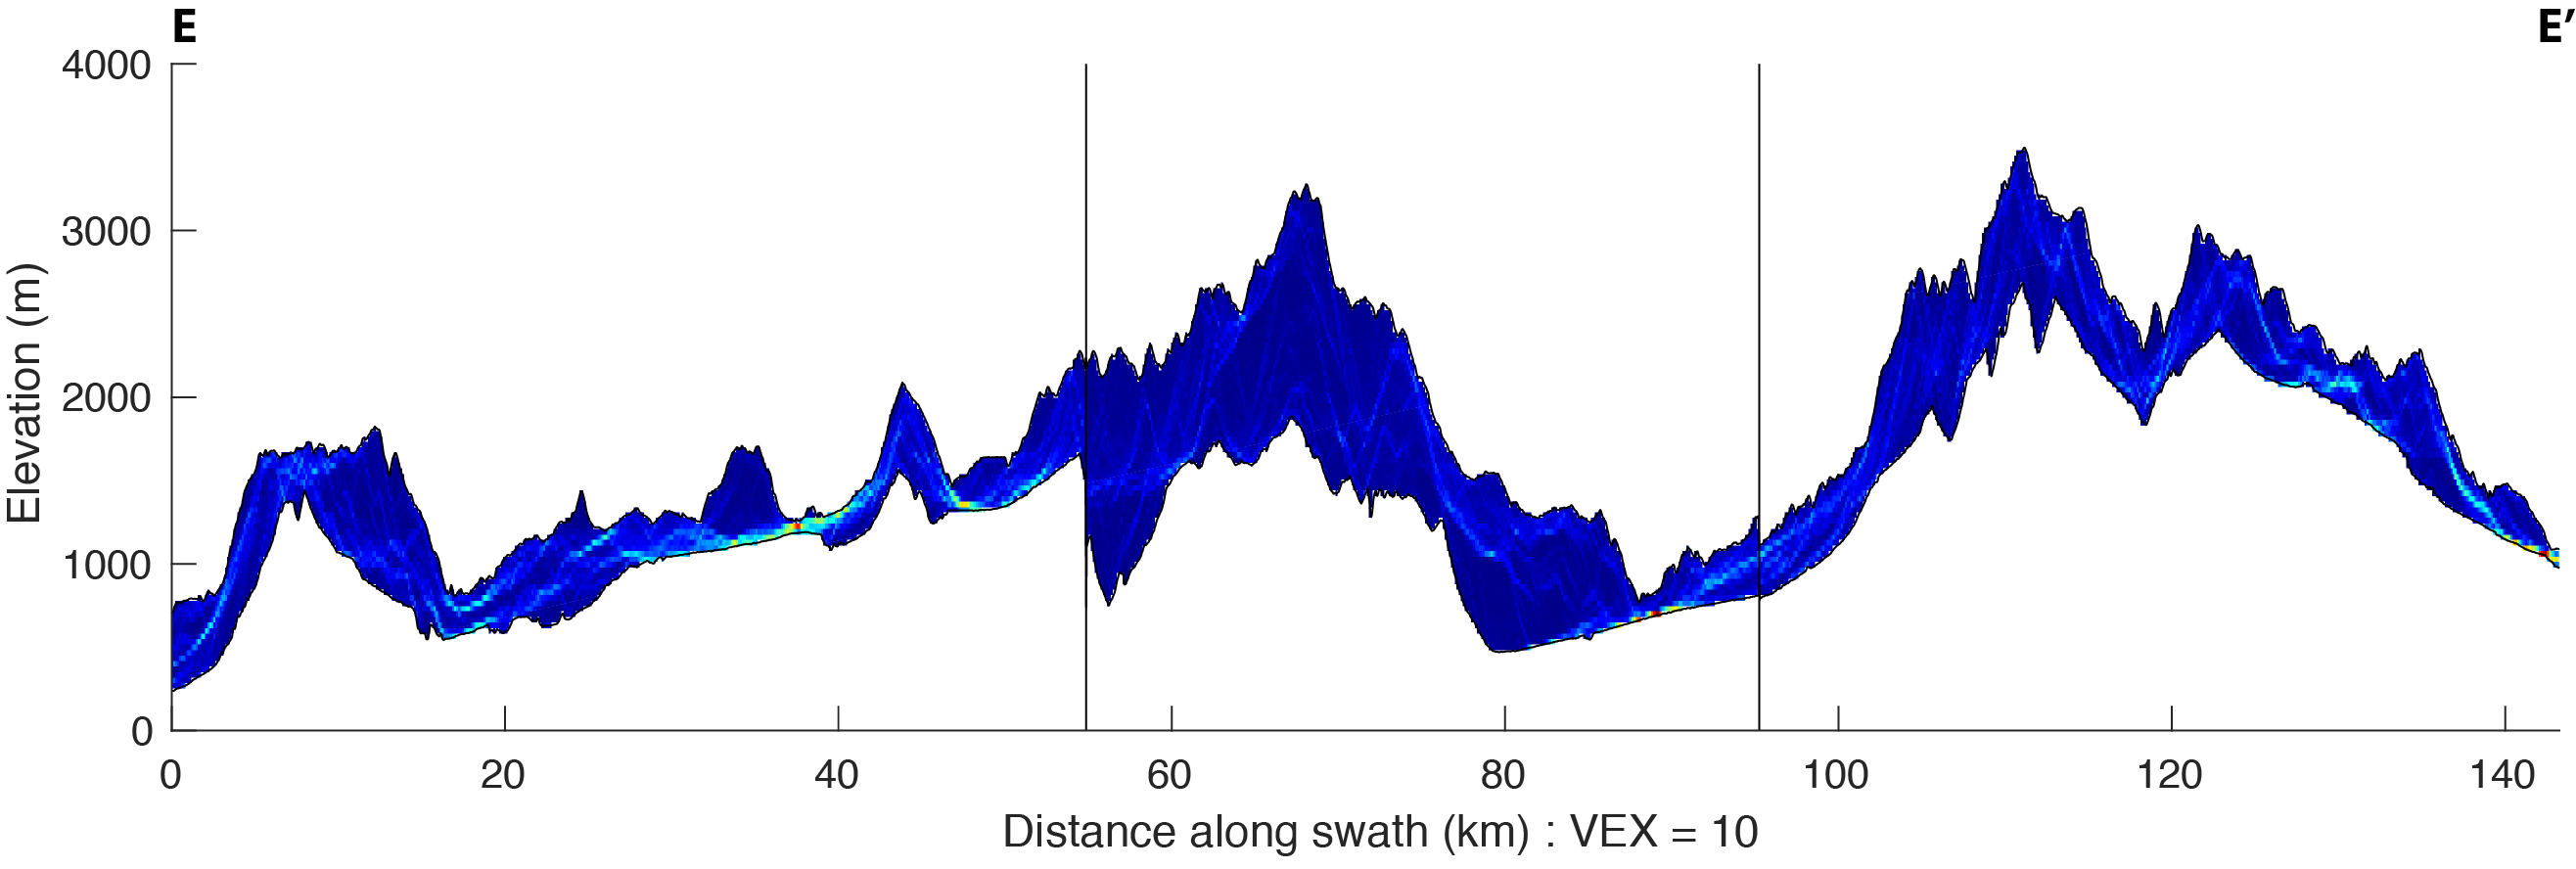
\includegraphics[width=16.5cm]{PNGs/Cross_SwathHeatmap.png}
	\caption{Swath output from \nameref{sec:Swath} showing the result of plotting as a heatmap colored by the density of points at a given elevation.}
	\label{fig:HeatSwath}
\end{figure}

\subsection{\textit{MakeCombinedSwath}} \label{sec:CombSwath}
\paragraph{}It can be useful to visualize additional data projected onto a swath profile. The \textit{MakeCombinedSwath} provides a flexible framework within which to produce such plots. There are a variety of types of data that can be plotted onto a swath profile:

\begin{itemize}
	\item \textit{'points3'} - generic point dataset with x, y, and z coordinates.
	\item \textit{'points4'} - generic point dataset with x, y, and z coordinates with an additional value. The resulting plots will color the points by this additional value.
	\item \textit{'points5'} - generic point dataset with x, y, and z coordinates with two additional values. The resulting plots will color the points by the first additional value and scale the points by the second value.
	\item \textit{'eqs'} - plot optimized for earthquakes for data with x, y, depth, and magnitude. Points will be scaled by magnitude and colored by the distance from the center of the swath line (e.g. Figure \ref{fig:EqSwath}).
	\item \textit{'STREAMobj'} - will project portions of a provided STREAMobj onto the swath.
	\item \textit{'ksn\_chandata'} - will project the \textit{k\textsubscript{sn}} values from a 'chandata' mat file produced by the old Profiler51 code (some of us have A LOT of these sitting around).
	\item \textit{'ksn\_batch'} - will project the \textit{k\textsubscript{sn}} values contained in the geographic data structure output from the \nameref{sec:KsnBatch} function.
	\item \textit{'ksn\_profiler'} - will project the \textit{k\textsubscript{sn}} values contained in the \textit{'knl'} array output from \nameref{sec:KsnProfiler}.
	\item \textit{'basin\_stats'} - will project basin data output from \nameref{sec:CompStats}. You must specify a quantity to color basins by with the \textit{'basin\_value'} parameter and can optionally also scale point size by an additional quantity with the \textit{'basin\_scale'} parameter (e.g. Figure \ref{fig:KsnSwath}).
	\item \textit{'basin\_knicks'} - will project knickpoint locations as produced by \nameref{sec:BsnKncks}.
\end{itemize}

\begin{figure}[H]
	\centering
	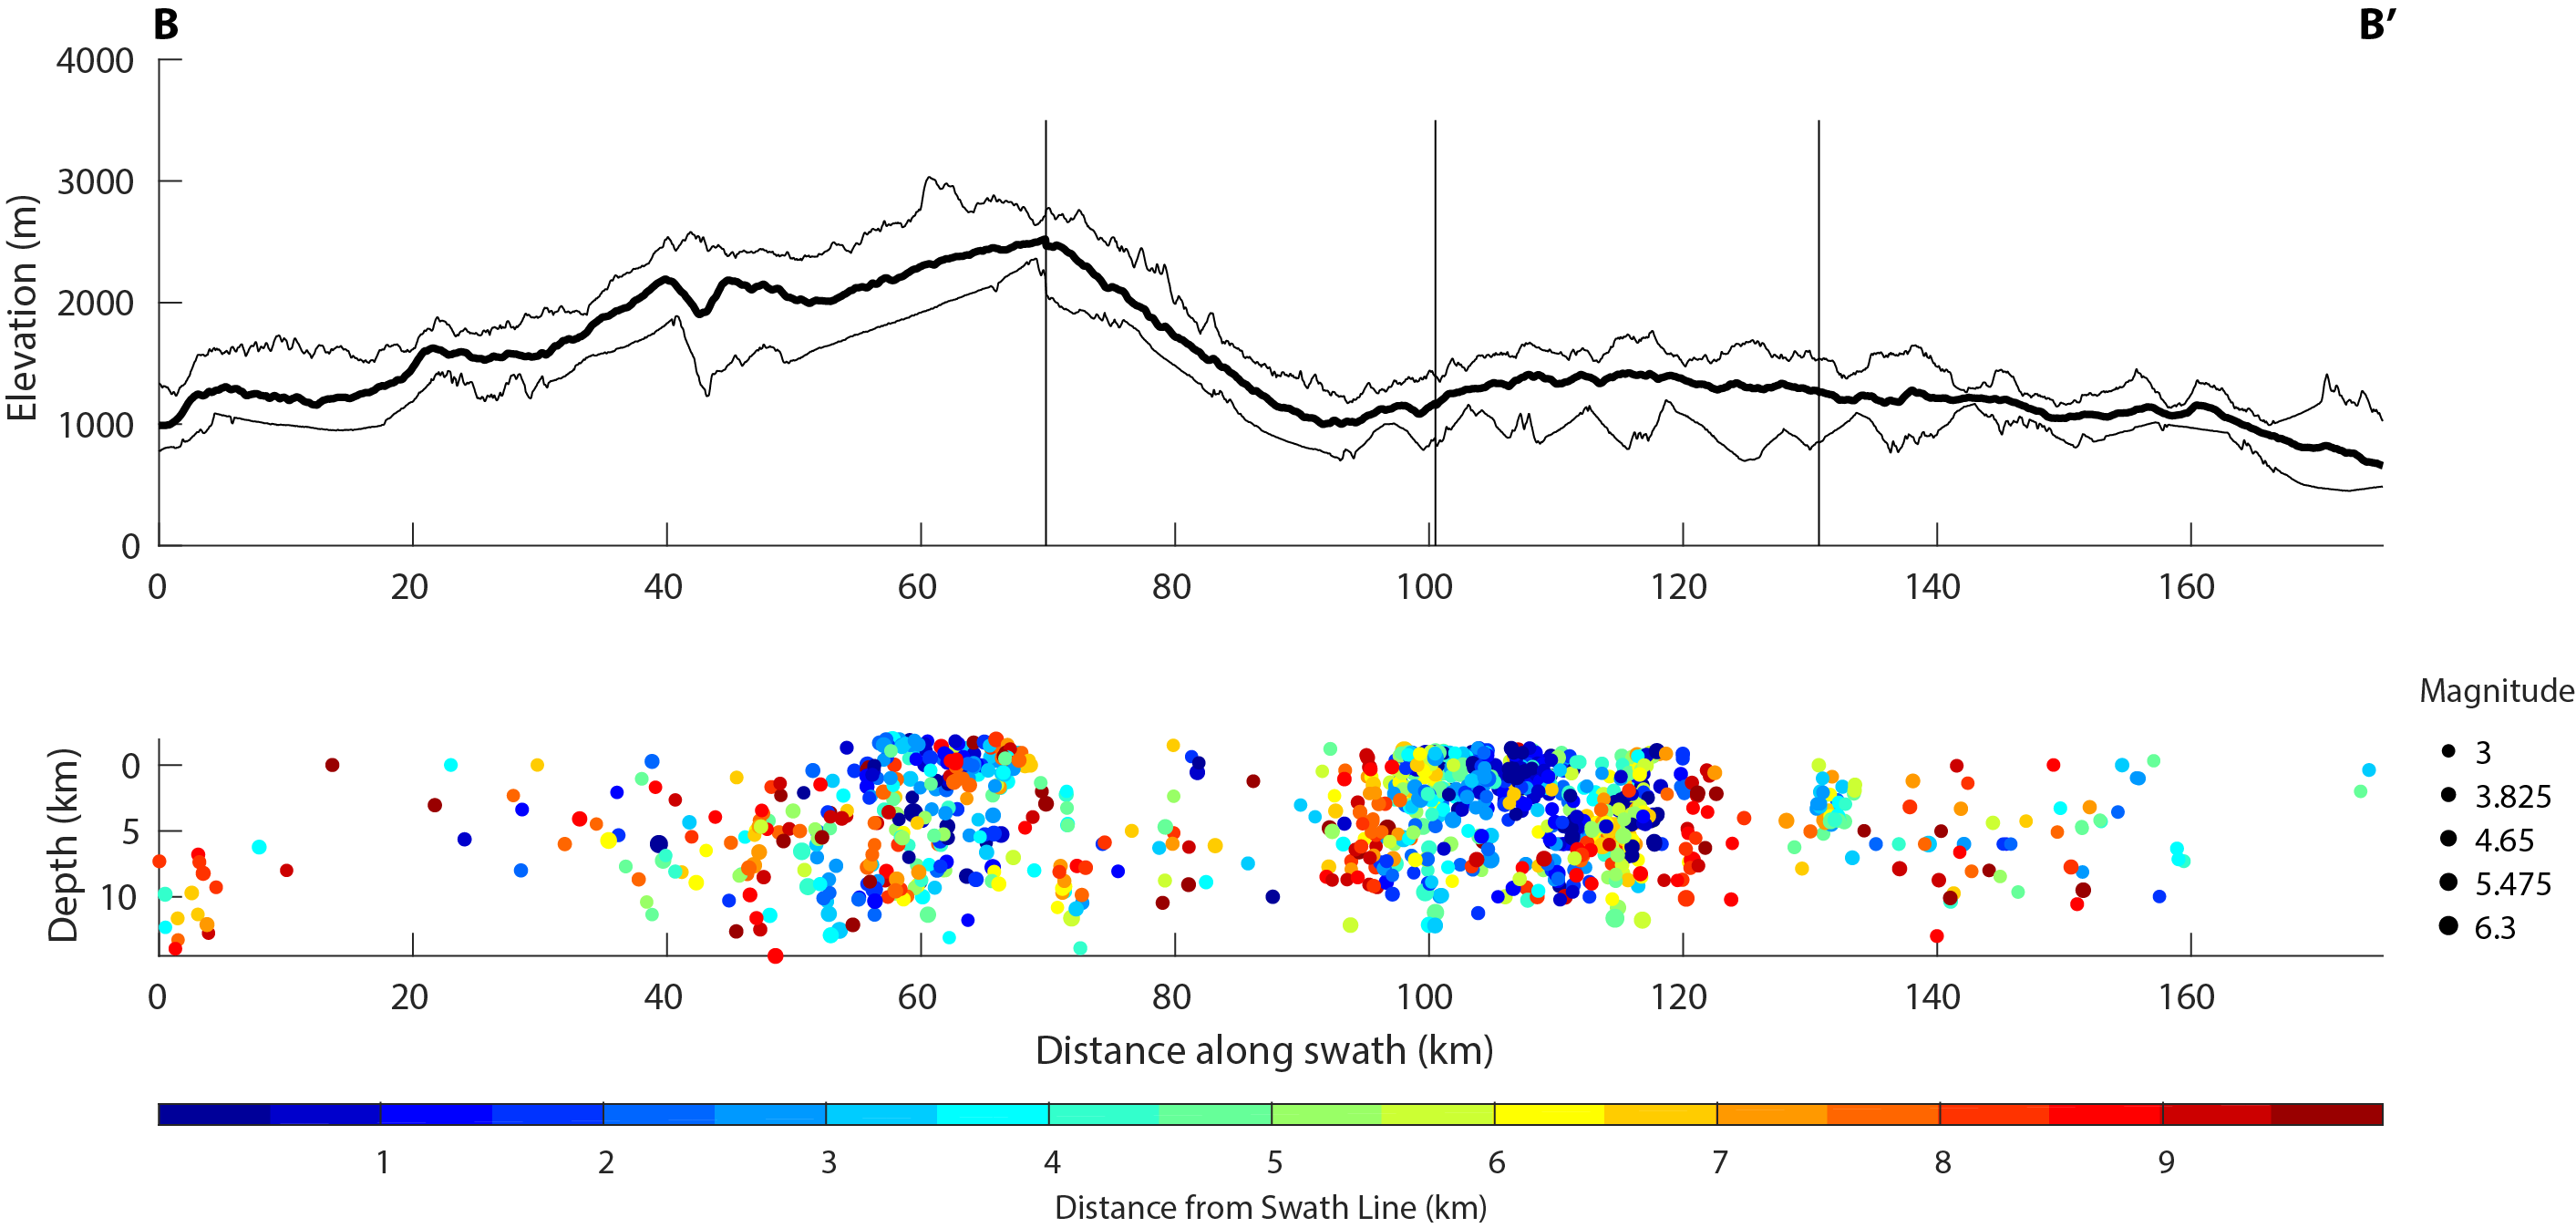
\includegraphics[width=16.5cm]{PNGs/SanBern_EQSwath.png}
	\caption{Swath output from \nameref{sec:CombSwath} projecting earthquake data}
	\label{fig:EqSwath}
\end{figure}

\begin{figure}[H]
	\centering
	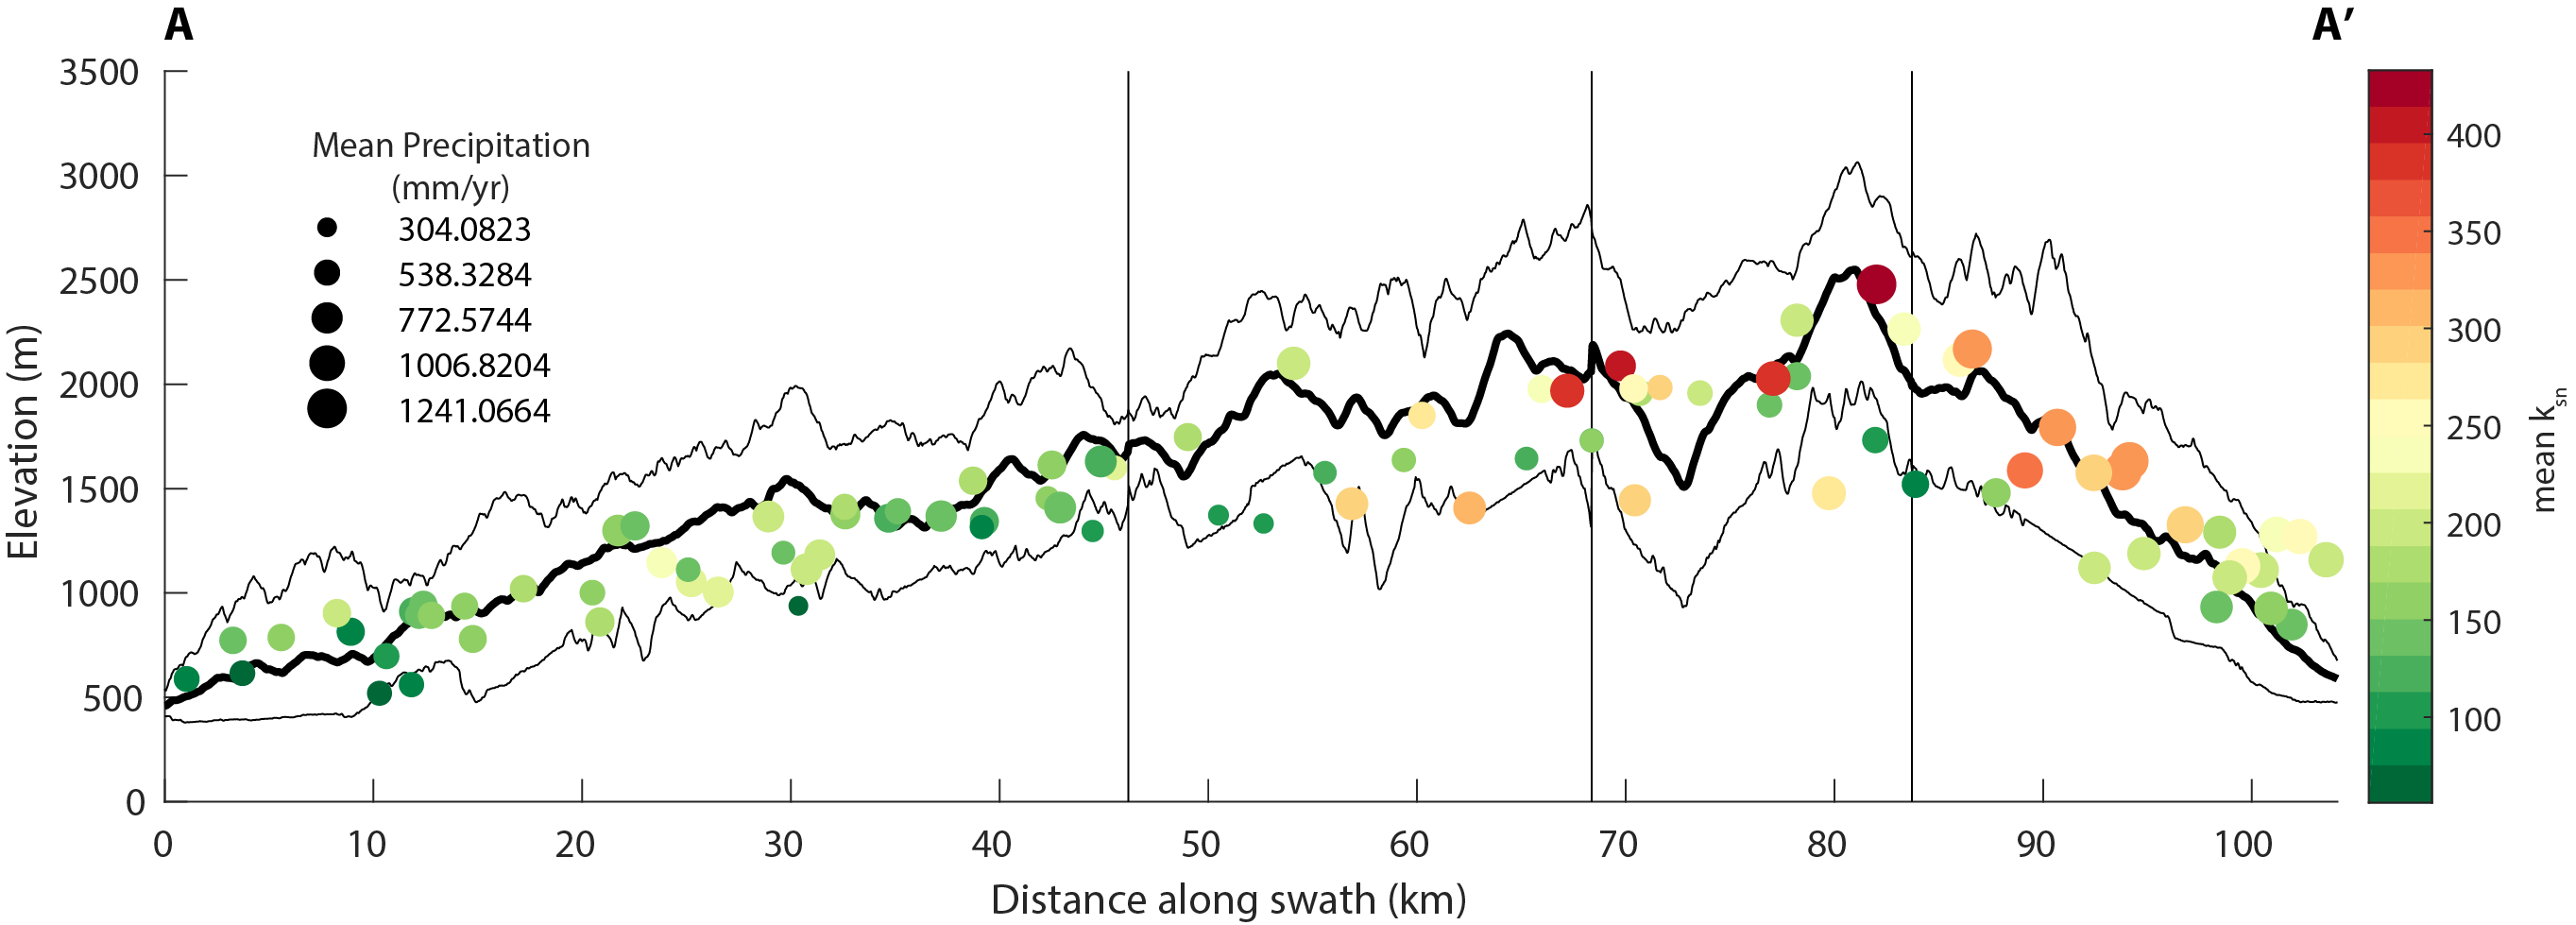
\includegraphics[width=16.5cm]{PNGs/SanGabes_KsnSwath.png}
	\caption{Swath output from \nameref{sec:CombSwath} projecting basin locations from \nameref{sec:CompStats} and colored by mean \textit{k\textsubscript{sn}} and scaled by mean precipitation.}
	\label{fig:KsnSwath}
\end{figure}

\paragraph{}Importantly, the \textit{MakeCombinedSwath} function is setup so that the width to sample the topography to produce the topographic swath is decoupled from the width from which to sample the provided data (you can of course make these equal if you want). By default the function will also plot a map displaying which data points are included in the projected data on the swath figure, you can suppress the drawing of this map with the optional \textit{'plot\_map'} parameter.

\subsection{\textit{MakeSerialSwath}} \label{sec:SerSwath}
\paragraph{}In some cases, it is useful to produce a series of swath profiles that are semi-parallel to each other or follow a particular path. The \textit{MakeSerialSwath} function is designed to make producing such a product simpler. As with \nameref{sec:Swath}, you must provide a base \textit{GRIDobj} from which to produce the swaths and a series of x-y points that will define the serial swaths, but in this case the swaths will be oriented perpendicular to the provided line. You can alternatively provide an empty array to this \textit{'points'} input to initiate a graphical choice within Matlab to create the base line. Through required and optional inputs you can control the length of individual swaths, the width of the swaths either by directly specifying the width in map units or by specifying the number of equal width swaths to create along the base line, and the orientation of the swaths with respect to the baseline (i.e should the swaths be centered along the baseline as in \nameref{fig:SerSwath} or aligned along the 'top' or 'bottom' of the baseline). 

\begin{figure}[H]
	\centering
	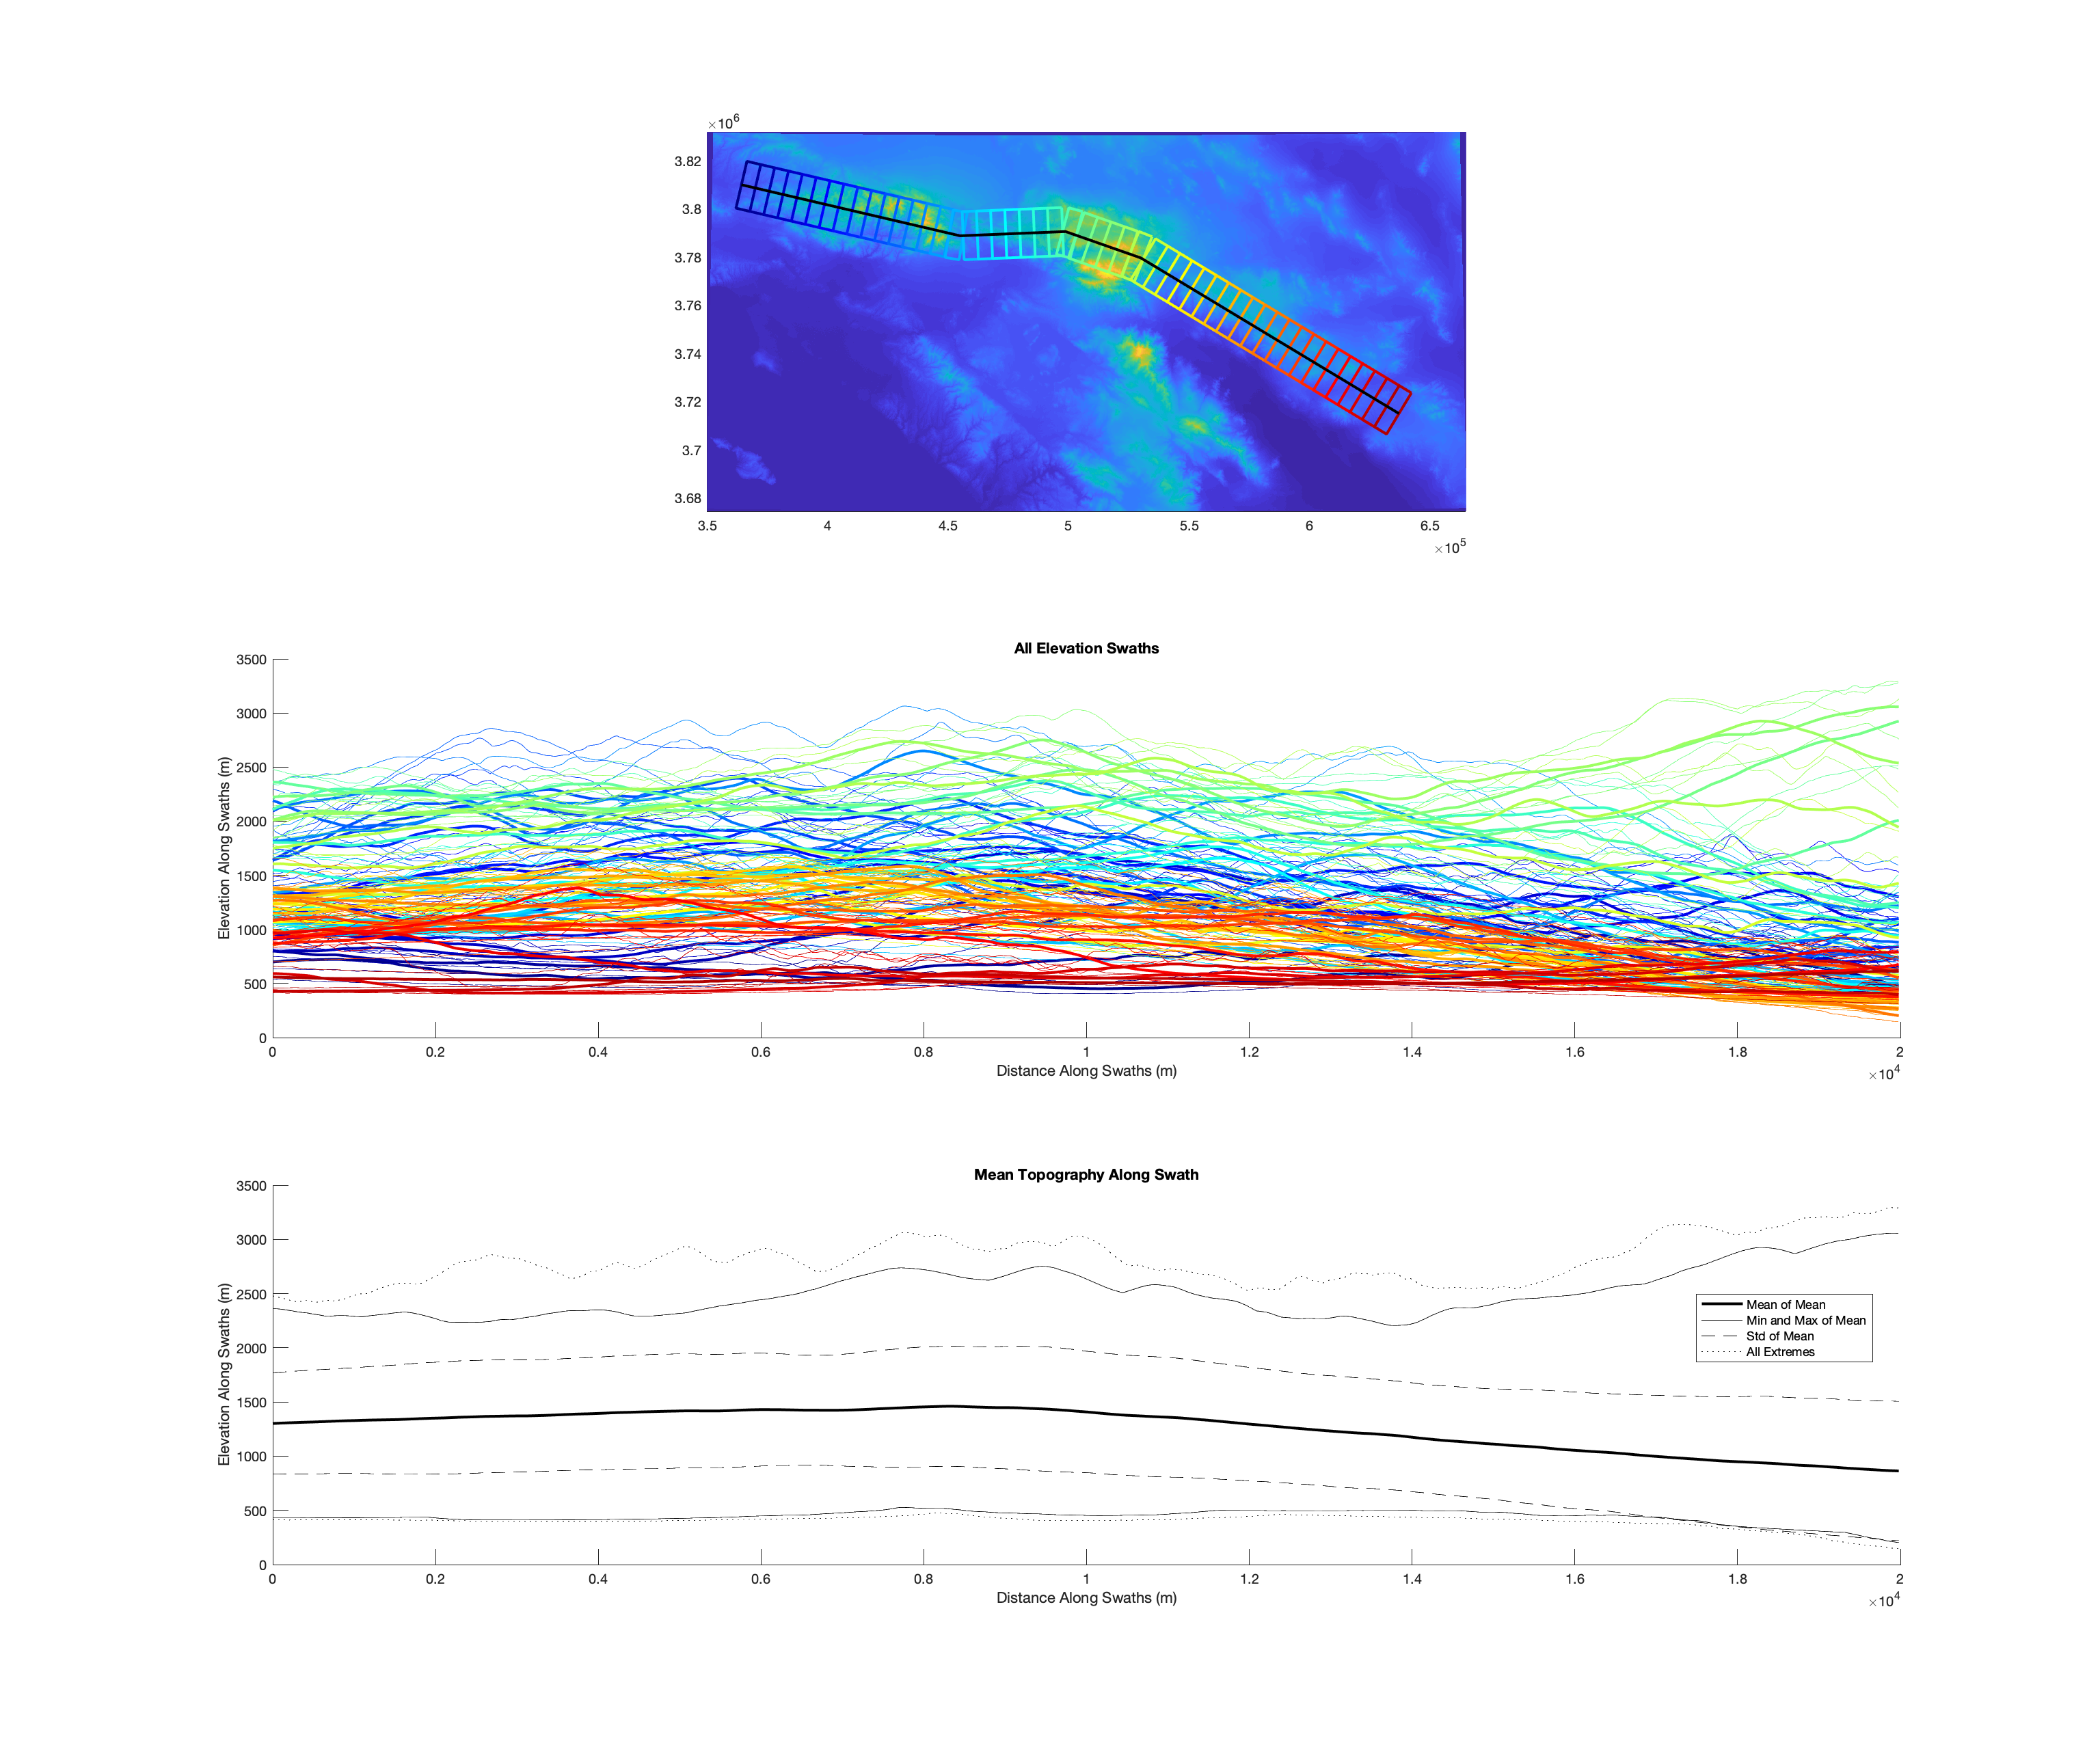
\includegraphics[width=14cm]{PNGs/SerialSwath.png}
	\caption{Standard graphic output from \nameref{sec:SerSwath} with a series of 50 equal width, 20 km long swaths, centered along the provided line (dark black line in the upper panel). The middle panel shows the minimum, mean, and maximum swath values for each swath (keyed by their color) and the bottom panel shows the average of all the swaths.}
	\label{fig:SerSwath}
\end{figure}

\paragraph{}The primary output of the \textit{MakeSerialSwath} function is a cell array containing individual \textit{SWATHobjs} created along the baseline. These individual \textit{SWATHobjs} are suitable for use in other functions, e.g. \nameref{sec:CombSwath} or plotting with built in \textit{TopoToolbox} function like \textit{plotdz}.

\subsection{\textit{ProjectOntoSwath}} \label{sec:ProjSwath}
\paragraph{}The \textit{ProjectOntoSwath} function is used in \nameref{sec:CombSwath} to do the data projection, but we include it as a separate function as it may be useful for users. \textit{ProjectOntoSwath} finds the distance of a list of x and y points along and from the centerline of a provided \textit{SWATHobj} based on a user defined width within which to sample the data. Distances of points that lie beyond the extent of the swath or lie outside of the data sampling width will be set to NaN. The function projects data onto each swath segment (i.e. if the swath line is bent) and finds the swath segment that data are closest to in tangential distance to avoid duplication of points. Note that there is no compiled version of \textit{ProjectOntoSwath}.

\subsection{\textit{ProjectSmallCircleOntoSwath}}
\paragraph{}This function is similar to \nameref{sec:ProjSwath}, but instead of projecting points along paths perpendicular to the swath, this function takes an input coordinate (in projected coordinates) to use as the center of a family of small circles along which to project the provided x-y points. This function can be used in combination with \nameref{sec:SmallCirc} if you need to first determine a small circle center that would be appropriate. As with \nameref{sec:ProjSwath}, the function outputs the location of points along the swath based on their projected positions. The function also calculates the distance from the point along the swath both in map units as measured along the small circle arc between the point and the swath center line and in degrees.

\subsection{\textit{ProjectGPSOntoSwath}}
\paragraph{}The \textit{ProjectGPSOntoSwath} behaves identically to \nameref{sec:ProjSwath} in terms of the projection of the provided x-y location onto the swath and similarly provides distance along and from the swath of those points, but it also takes velocity and associated uncertainties (assumed to be in the standard north and east components) and projects those onto the swath. The output of the function gives the magnitude of the projected GPS vector, i.e. the magnitude of the velocity if resolved onto a plane parallel to the \textit{SWATHobj} and the associated uncertainty, i.e. the radius of a slice through the error ellipse at the orientation of the \textit{SWATHobj}. The function also provides north and east components for this projected vector which would be suitable inputs to the \textit{quiver} function for plotting.

\subsection{\textit{CrossSwath}}
\paragraph{}Often, it is useful to precisely determine where a particular linear feature crosses a \textit{SWATHobj} for plotting purposes. This function takes a \textit{SWATHobj} and a line (defined by a series of x-y points at the vertices of the line in question) and calculates the positions along a swath where the line crosses the bounds of the swath (in both x-y coordinates and distance along the swath) and the mean crossing location of the line. 

%%%%%%%%
\section{Miscellaneous}

\subsection{\textit{BestFitSmallCircle}} \label{sec:SmallCirc}
\paragraph{}Function to find the best fit small circle for a set of provided x-y points. In addition to the x and y coordinates, you are expected to provided the projection information for the x and y coordinates as a structure. Assuming you have a \textit{GRIDobj} with which these x-y points are associated, the necessary projection information (i.e. the input for the \textit{'proj'} argument) is stored in the \textit{DEM.georef.mstruct} or alternatively, if you are using an older version of TopoToolbox, \textit{DEM.georef}. This information can also be directly extracted from a GeoTIFF with the \textit{geotiffinfo} function. If you provide an empty array to the textit{'proj'} argument, the function assumes that the provided x-y points are already geographic coordinates. The function will output the center of the best fit small circle (in geographic coordinates), the radius of the small circle (in degrees), and a series of points along the perimeter of the small circle (in projected coordinates unless the original points are provided as geographic)

\begin{lstlisting}[language=Matlab]
% Produce a best fit small circle from a series of x and y coordinates extracted from a particular DEM
[clat,clon,crad,cpx,cpy]=BestFitSmallCircle(x,y,DEM.georef.mstruct);
% Alternatively, grab the projection info directly from a geotiff
proj=geotiffinfo('srtm_bigtujunga30m_utm11.tif');
[clat,clon,crad,cpx,cpy]=BestFitSmallCircle(x,y,proj);
% You can use the built in projinv and projfwd functions to convert the clat and clon or cpx and cpy outputs
[center_x,center_y]=projfwd(proj,clat,clon); % Convert center to projected
[cp_lat,cp_lon]=projinv(proj,cpx,cpy); % Convert perimeter to geographic
\end{lstlisting}

\subsection{\textit{ksncolor}} \label{sec:ksncolor}
\paragraph{}Function to generate a colormap that roughly approximates the stereotypical green-yellow-red color progression commonly used for \textit{k\textsubscript{sn}} data in publications, see Figure \ref{fig:KsnSwath} for an example of the color map. Note that there is no compiled version of \textit{ksncolor}.

\subsection{\textit{PlotKsn}} \label{sec:plotksn}
\paragraph{}The \textit{PlotKsn} function will quickly plot a stream network colored by \textit{k\textsubscript{sn}} overlaying a hillshade colored by elevation. Uses the \nameref{sec:ksncolor} colormap. You can provide a valid geographic data structure output from \nameref{sec:KsnBatch} or  \nameref{sec:PrcRvBsn} or a shapefile output from \nameref{sec:KsnBatch}, \nameref{sec:KsnProfiler}, or  \nameref{sec:PrcRvBsn}. Optionally can also include a set of knickpoints output from \nameref{sec:PrcRvBsn} or \nameref{sec:BsnKncks} to plot knickpoint locations. 

\subsection{\textit{DippingBedFinder}} \label{sec:BedFinder}
\paragraph{}\textit{DippingBedFinder} is a simple function to estimate where a planar dipping bed should occur within a landscape based on a known occurrence and some information about the bed (Figure \ref{fig:Bed}). Specifically, you need to provide a location for the observation, a total thickness for the bed, an estimate of the height above the base of the bed at the point of observation, the strike of the bed (it's assumed you give this using the right hand rule), and the dip of the bed. 

\begin{figure}[H]
	\centering
	\begin{subfigure}{.5\textwidth}
		\centering
		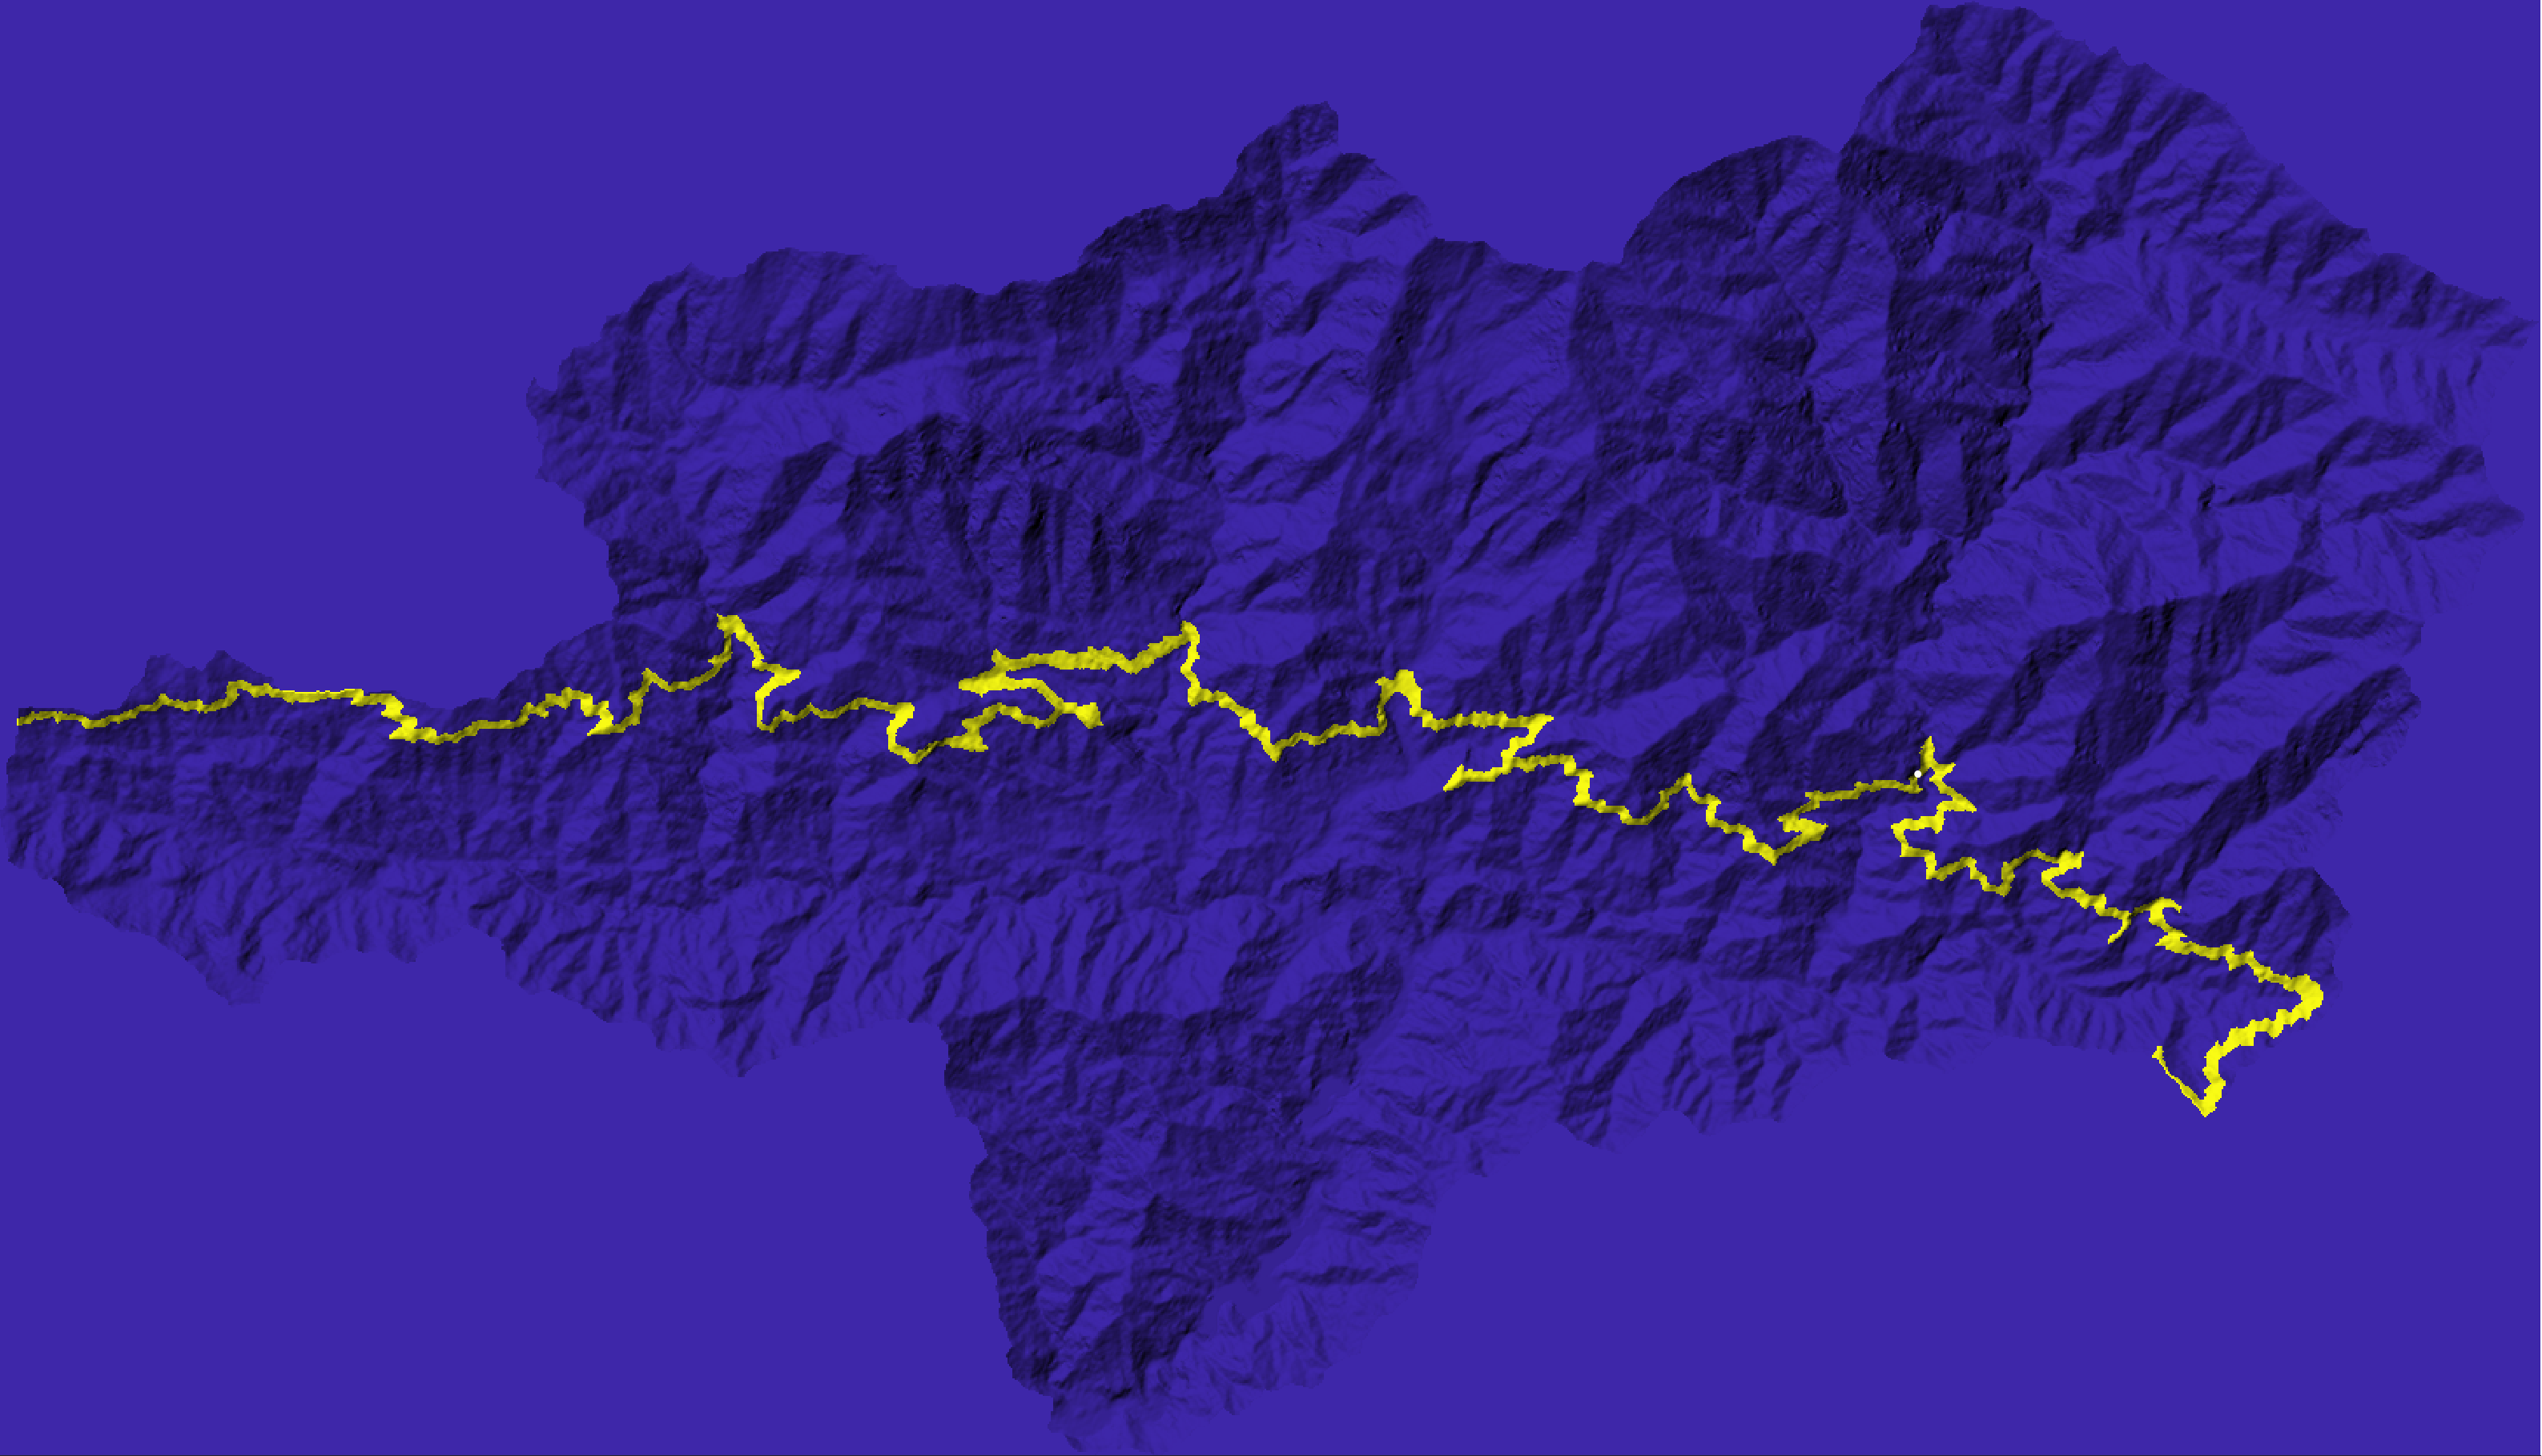
\includegraphics[width=.8\linewidth]{PNGs/Bed1.png}
		\caption{Projection of a 100 meter thick bed, 50 meters up from the base.}
		\label{fig:BedSub1}
	\end{subfigure}%
	\begin{subfigure}{.5\textwidth}
		\centering
		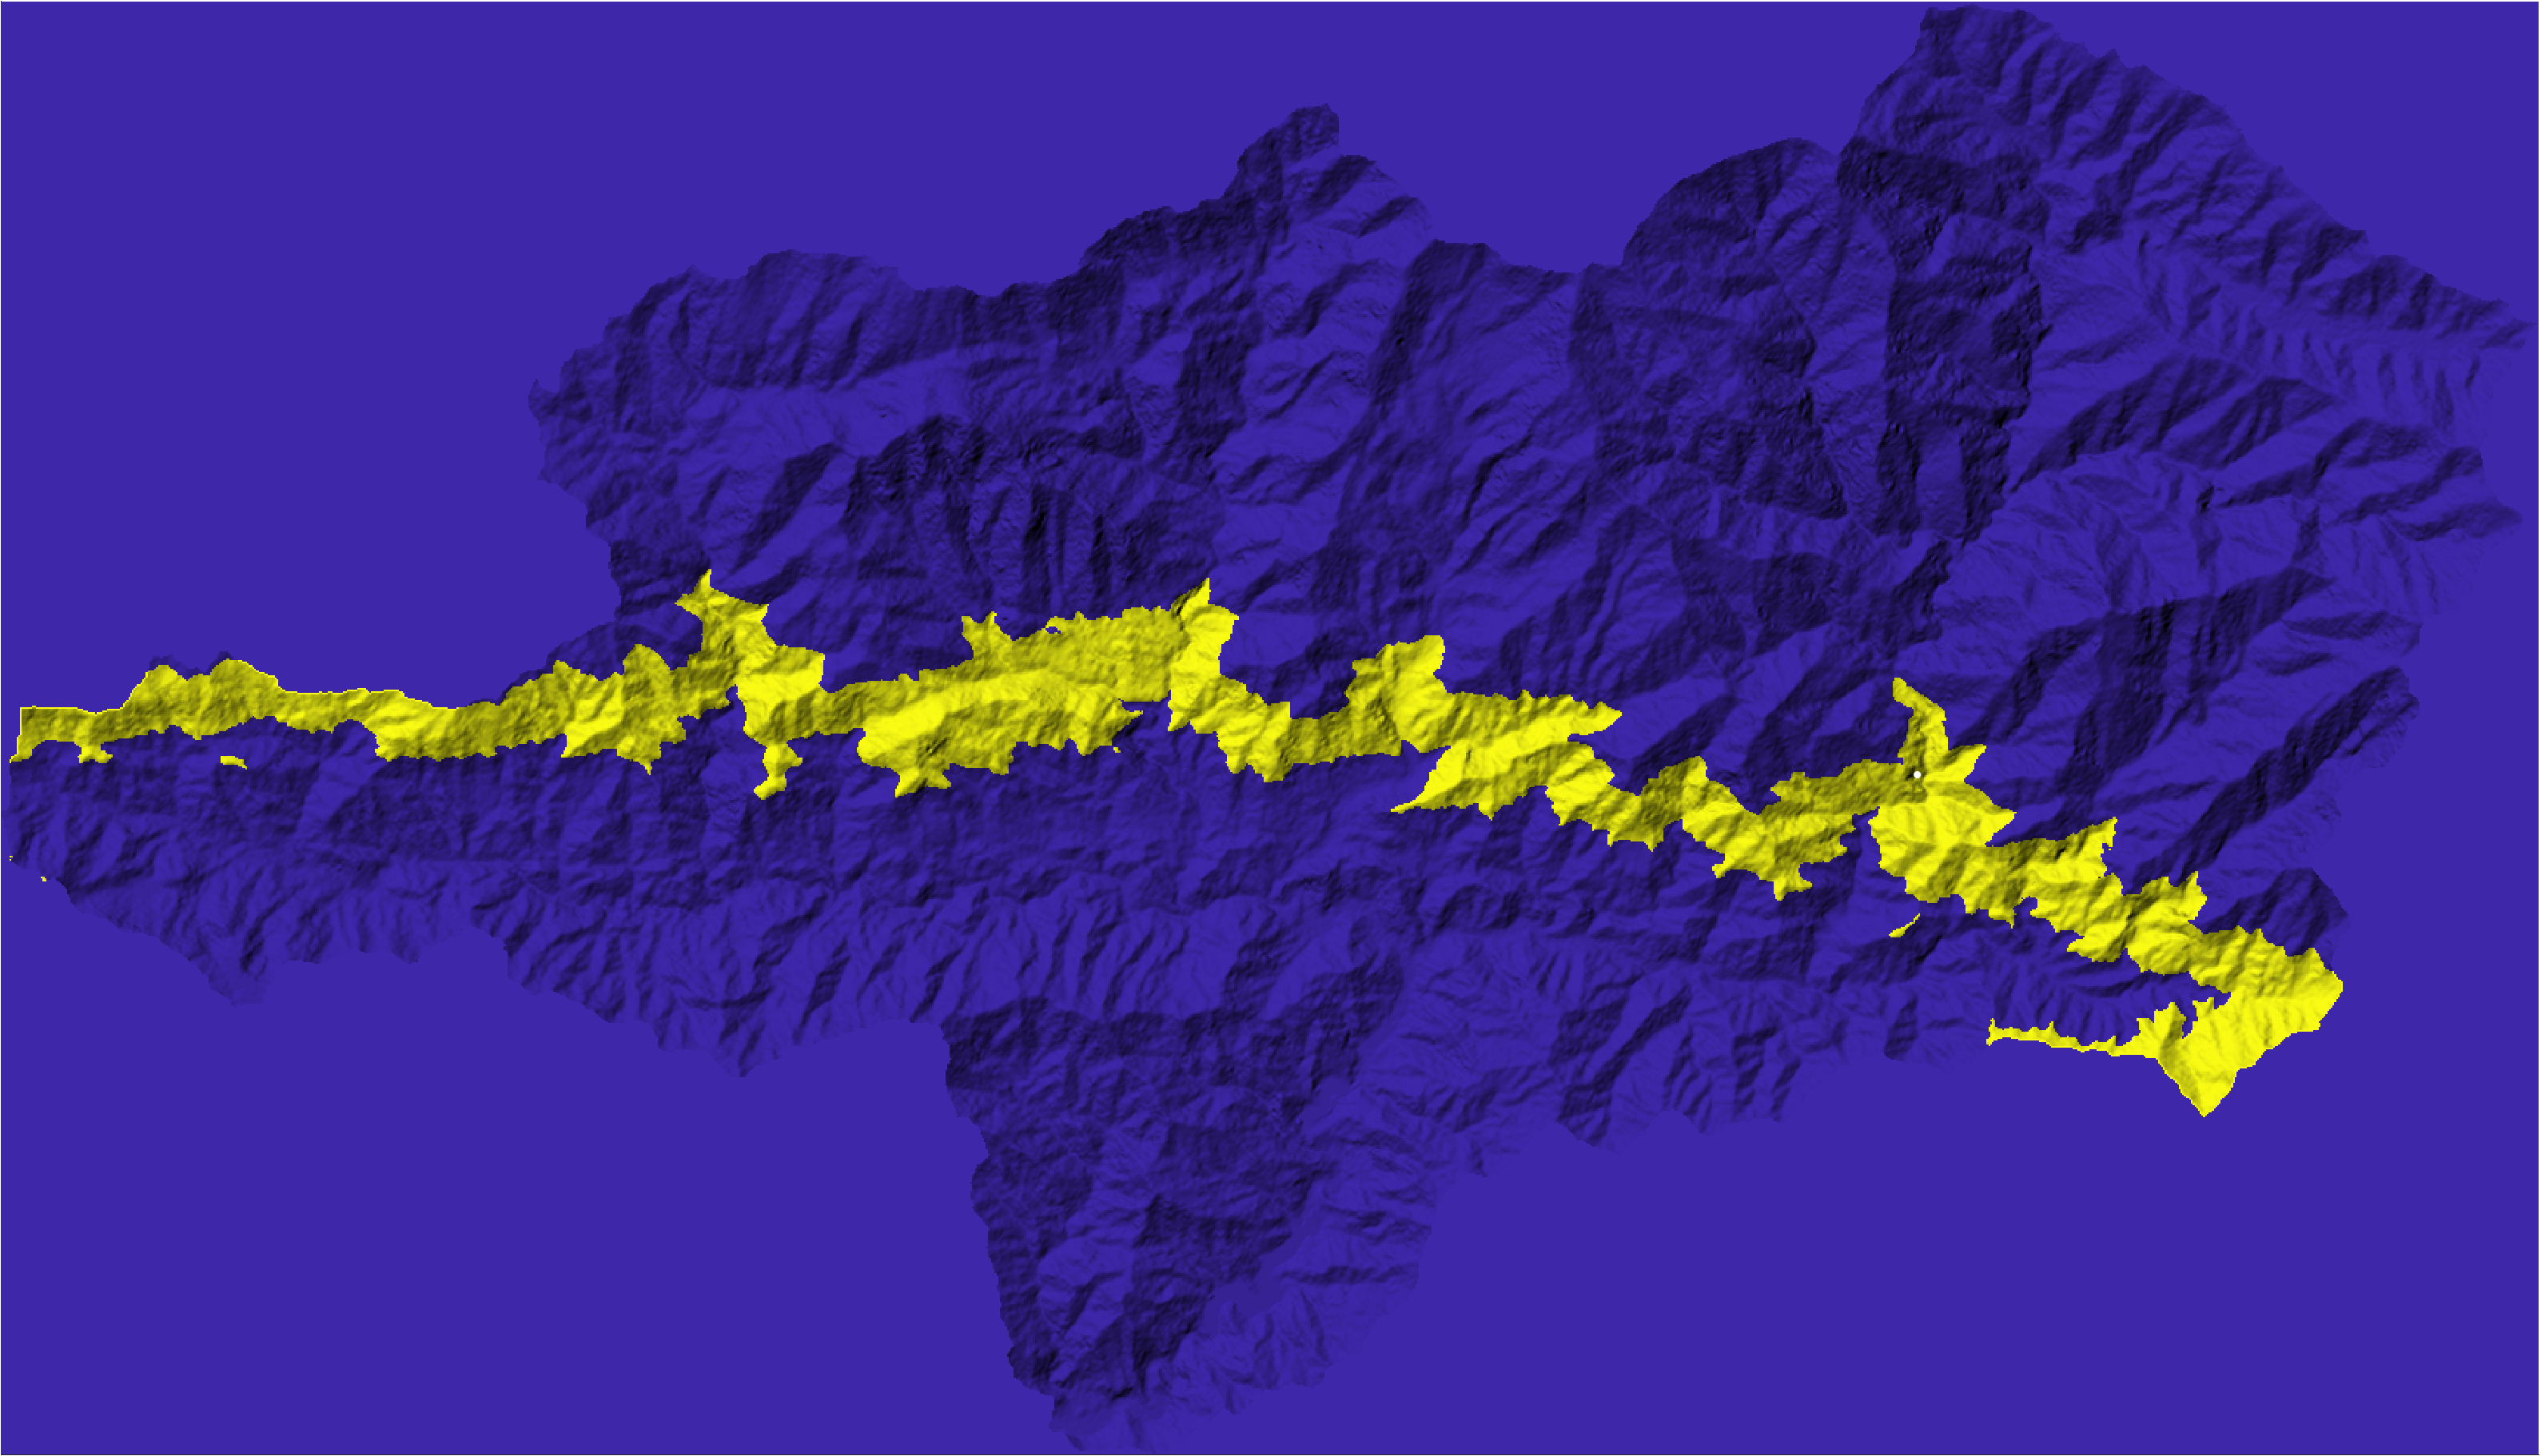
\includegraphics[width=.8\linewidth]{PNGs/Bed2.png}
		\caption{Projection of a 500 meter thick bed, 250 meters up from the base.}
		\label{fig:BedSub2}
	\end{subfigure}
	\caption{Example outputs from \nameref{sec:BedFinder} for a bed striking 280\textdegree and dipping 10\textdegree.}
	\label{fig:Bed}
\end{figure}

\paragraph{}You can provide an empty array for the location of observation to choose a point on the provided DEM to use as the location. The location of the observation is marked on the figure with a white dot.

\subsection{\textit{HackRelationship}}
\paragraph{}Temporary

\subsection{\textit{Mat2Arc}} \label{sec:Mat2Arc}
\paragraph{}\textit{Mat2Arc} is a helper function that takes any matfile as an input and will search its contents and produce either ESRI ascii grids or geotiffs and shapefiles from any valid datasets. Specifically, will make ascii grids or geotiffs of any \textit{GRIDobj}, will convert any \textit{FLOWobj} to an Arc style flow raster an export as an ascii grid or geotiff, and output any \textit{STREAMobj} or recognizable geographic data structure as a shapefile. Whether rasters are saved as ESRI ascii grids or geotiffs is controlled with the optional \textit{'raster\_type'} parameter.

% Uncomment to regenerate bbl file
\bibliography{TAKmanualREF.bib}

\appendix

%%%%%%%%%%%%%%%%%%%%%
\section{Headers for Compiled Functions}\label{sec:CmpFuncCalls}
\paragraph{} The following section reproduces the headers of each compiled function. Please refer to the \nameref{sec:CmpFunc} section of the user manual for additional information on how to use the compiled versions of the functions.

\subsection{Basin2Raster}
\paragraph{Description:}
Function takes outputs from 'ProcessRiverBasins' function and produces a single GRIDobj with individual drainage
basins (as selected by 'ProcessRiverBasins' and 'SubDivideBigBasins') assinged various values

\paragraph{Required Inputs:}
\begin{itemize}
\item wdir - full path of working directory
\item MakeStreamsMat - full path of the matfile provided as an input to cmpProcessRiverBasins
\item valueOI - value to assign to basins, acceptable inputs are:
\begin{itemize}
\item 'ksn' - mean ksn value of basin
\item 'gradient' - mean gradient of basin
\item 'elevation' - mean elevation of basin
\item 'relief' - mean relief of basin (must specify the radius of interest with the 'relief\_radius' parameter)
\item 'chir2' - R\textsuperscript{2} value of chi-z fit (proxy for disequilibrium)
\item 'drainage\_area' - drainage area in km2 of basin
\item 'hypsometric\_integral' - hypsometric integral of basin
\item 'id' - basin ID number (i.e third column RiverMouth output)
\item 'theta' - best-fit concavity resultant from the topo toolbox chiplot function 
\item 'NAME' - where name is the name provided for an extra grid (i.e. entry to second column of 'add\_grid' or entry to 
third column of 'add\_cat\_grid'), value input will be mean for additional grid names or mode for additional 
categorical grid names
\end{itemize}
\item location\_of\_data\_files - full path of folder which contains the mat files from 'ProcessRiverBasins' as a string
\end{itemize}

\paragraph{Optional Inputs:}
\begin{itemize}
\item file\_name\_prefix ['basins'] - prefix for outputs, will automatically append the type of output, i.e. 'ksn', 'elevation', etc
\item location\_of\_subbasins ['SubBasins'] - name of folder that contains subbasins of interest (if you created subbasins using
"SubDivideBigBasins"), expected to be within the main Basin folder provided with "location\_of\_data\_files".
\item method ['subdivided'] - method used for subdividing watersheds. If you used 'ProcessRiversBasins' and then
'SubDivideBigBasins' or if you only used 'ProcessRiverBasins' but did not pick any nested catchments, i.e.
none of the river mouths supplied to 'ProcessRiverBasins' were within the catchment boundaries of other 
watersheds for which you provided river mouths, then you should use use 'subdivided' which is the default
so you do not need to specify a value for this property. If you picked nested catchments manually and then
ran 'ProcessRiverBasins' you should use 'nested'.
\item relief\_radius [2500] - relief radius to use if 'valueOI' is set to 'relief'
\end{itemize}

\paragraph{Examples} if running for the command line, minus OS specific way of calling main TAK function:

\begin{lstlisting}[language=bash]
Basin2Raser /path/to/wdir MakeStreams.mat ksn MainBasins
Basin2Raster /path/to/wdir MakeStreams.mat ksn MainBasins location_of_subbasins MySubbasins file_name_prefix Test
\end{lstlisting}

\subsection{Basin2Shape} \label{sec:CmpBsn2Shp}

\paragraph{Description:}
Function to take the outputs from 'ProcessRiverBasins' and 'SubDivideBigBasins' and produce a single shapefile showing the outlines of polygons
and with commonly desired attributes from the results of 'ProcessRiverBasins' etc. See below for a full list of fields that the output shapefile
will include. If additional grids were provided to 'ProcessRiverBasins', mean and standard error values for those grids will be auto-populated in
the shapefile and the name of the fields will be the character array provided in the second column of additional grids input. This function also
allows you to input a list of additional fields you wish to include (see Optional Inputs below). If you would rather create a GRIDobj with specified
values, use 'Basin2Raster'.

\paragraph{Required Inputs:}
\begin{itemize}
\item wdir - full path of working directory
\item MakeStreamsMat - name of the matfile provided as an input to cmpProcessRiverBasins
\item location\_of\_data\_files - name of folder which contains the mat files from 'ProcessRiverBasins'
\end{itemize}

\paragraph{Optional Inputs:}
\begin{itemize}
\item location\_of\_subbasins ['SubBasins'] - name of folder that contains subbasins of interest (if you created subbasins using
"SubDivideBigBasins"), expected to be within the main Basin folder provided with "location\_of\_data\_files". Note that if you do not provide
the correct directory name for the location of the subbasins, subbasin values will not be included in the output regardless of your choice
for the "include" parameter.
\item shape\_name ['basins'] - name for the shapefile to be export, must have no spaces to be a valid name for ArcGIS and should NOT include the '.shp'
\item include ['all'] - parameter to specify which basins to include in building the shapfile. The default 'all' will include all basin mat files in the 
folder you specify. Providing 'subdivided' will check to see if a given main basin was subdivided using 'SubdivideBigBasins' and then only include 
the subdivided versions of that basin (i.e. the original main basin for those subbasins will not be included in the shapefile). Providing 'bigonly'
will only include the original basins produced by 'ProcessRiverBasins' even if 'SubDivideBigBasins' was run. If 'SubDivideBigBasins' was never run,
result of 'all' and 'bigonly' will be the same.
\item extra\_field\_values [] - name text file of extra field values you wish to include. The first column in this file must be the river basin number
(i.e. the identifying number in the third column of the RiverMouth input to ProcessRiverBasins or the number generated for the basin in
SubDivideBigBasins). Only one row per river basin number is allowed and ALL river basin numbers in the basins being processed must have a value
associated with them. Additional columns are interpreted as the values with which you wish to populate the extra fields. These can either be character
arrays or numbers, other values will results in an error. The function will use the header names within this file to name fields in the output shapefile
\item new\_concavity [] - a 1 x m array of concavity values to recalculate normalized channel steepness statistics (mean, standard error and/or standard deviation) using the
provided concavities.
\item uncertainty ['se'] - parameter to control which measure of uncertainty is included, expects 'se' for standard error (default), 'std' for standard deviation, or 'both'
to include both standard error and deviation.
\item populate\_categories [false] - logical flag to add entries that indicate the percentage of a watershed occupied by each category from a categorical grid, e.g. if you
provided an entry for 'add\_cat\_grids' to ProcessRiverBasins that was a geologic map that had three units, 'Q', 'Mz', and 'Pz' and you set 'populate\_categories' 
to true there will be field names in the resulting shapefile named 'Q', 'Mz', and 'Pz' and the values stored in those columns will correspond to the percentage 
of each basin covered by each unit for each basin. Setting populate\_categories to true will not have any effect if no entry was provided to 'add\_cat\_grids' when
running ProcessRiverBasins.
\end{itemize}

\paragraph{Output:}
\begin{itemize}
\item Saves a shapefile with the following default fields:
\begin{itemize}
\item river\_mouth - river mouth number provided to ProcessRiverBasins
\item drainage\_area - drainage area of basin in km\textsuperscript{2}
\item center\_x - x coordinate of basin in projected coordinates
\item center\_y - y coordinate of basin in projected coordinates
\item outlet\_elevation - elevation of pour point in m
\item mean\_el - mean elevation of basin in meters
\item max\_el - maximum elevation of basin in meters
\item mean\_ksn - mean channel steepenss
\item mean\_gradient - mean gradient
\end{itemize}
\item Either standard errors, standard deviations or both will be populated for elevation, ksn, and gradient depending on value of 'uncertainty'
\item Mean and standard error / standard deviation / both values will be populated for any additional grids
\end{itemize}

\paragraph{Examples} if running for the command line, minus OS specific way of calling main TAK function:
\begin{lstlisting}[language=bash]
Basin2Shape /path/to/wdir MakeStreams.mat MainBasins
Basin2Shape /path/to/wdir MakeStreams.mat MainBasins location_of_subbasins MySubbasins include subdivided	
\end{lstlisting}

\subsection{BasinPicker}
\paragraph{Description:}
Function takes results of makes streams and allows for interactive picking of basins (watersheds). Function was
designed intially for choosing basins suitable for detrital analyses (e.g. Be-10 cosmo). Displays two panel figure 
with topography colored by elevation and local relief on which to pick individual basins. After the figure displays,
it will wait until you press enter to begin the watershed picking process. This is to allow you to zoom, pan, etc to 
find a stream you are interested in. When you click enter, cross hairs will appear in the elevation map so you can 
select a pour point. Once you select a pour point, a new figure will display this basin and stream to confirm that's 
the watershed you wanted (it will also display the drainage area). You can either accept this basin or reject it if 
it was misclick. If you accept it will then display a new figure with the chi-z and longitudinal profiles for that basin. 
It will then give you a choice to either save the choice or discard it. Finally it will ask if you want to keep picking 
streams, if you choose yes (the default) it will start the process over. Note that any selected (and saved) pour point 
will be displayed on the main figure. As you pick basins the funciton saves a file called 'Outlets.mat' that contains 
the outlets you've picked so far. If you exit out of the function and restart it later, it looks for this Outlets file
in the current working directory so you can pick up where you left off.

\paragraph{Required Inputs:}
\begin{itemize}
\item wdir - full path of working directory
\item MatFile - Full path of matfile output from either 'cmpMakeStreams' or the name of a single basin mat file from 'cmpProcessRiverBasins'
\end{itemize}

\paragraph{Optional Inputs:}
\begin{itemize}
\item ref\_concavity [0.50]- reference concavity for chi-Z plots
\item rlf\_radius [2500] - radius in map units for calculating local relief
\item extra\_grid [] - sometimes it can be useful to also view an additional grid (e.g. georeferenced road map, precipitation grid, etc) along 
with the DEM and relief. The arugment provided should be the name of the extra grid of interest. This grid can be a different 
size or have a different cellsize than the underlying dem (but still must be the same projection and coordinates system!), it will be
resampled to match the provided DEM. 
\item cmap ['landcolor'] - colormap to use for the displayed maps. Input can be the name of a standard Matlab colormap 
\item conditioned\_DEM [] - option to provide a hydrologically conditioned DEM for use in this function, expects the mat file as saved by 'cmpConditionDEM'
See 'cmpConditionDEM' function for options for making a hydrological conditioned DEM. If no input is provided the code defaults to using the 
mincosthydrocon function.
\item interp\_value [0.1] - value (between 0 and 1) used for interpolation parameter in mincosthydrocon (not used if user provides a conditioned DEM)
\item plot\_type ['vector'] - expects either 'vector' or 'grid', default is 'vector'. Controls whether all streams are drawn as individual lines ('vector') or if
the stream network is plotted as a grid and downsampled ('grid'). The 'grid' option is much faster for large datasets, 
but can result in inaccurate site selections. The 'vector' option is easier to see, but can be very slow to load and interact with.
\item threshold\_area [1e6] - used to redraw downsampled stream network if 'plot\_type' is set to 'grid'
\item refine\_positions [] - expects the name of a text file containing a m x 2 array of x y positions that are near stream networks that you want to manually snap to the appropriate stream network. An example would be a series of GPS positions of river samples that don't quite lie on the stream network as determined by flow routing.
If you provide an entry for 'refine\_positions', the code will iteratively work through the provided points, displaying their location one point
at a time along with a zoomed inset window (size controlled by 'window\_size') on which you can precisely position the river mouth location.
\item window\_size [1] - size of inset window (in km) if you have provided an entry for 'refine\_positions'
\end{itemize}

\paragraph{Outputs:}
\begin{itemize}
\item Outlets - n x 3 matrix of sample locations with x coordinate, y coordinate, and basin ID number (valid input to 'ProcessRiverBasins'
as 'river\_mouths' parameter) saved as a mat file (for continuing a cmpBasinPicker run) and a text file
\end{itemize}

\paragraph{Examples} if running for the command line, minus OS specific way of calling main TAK function:
\begin{lstlisting}[language=bash]
BasinPicker /path/to/wdir Topo.mat
BasinPicker /path/to/wdir Topo.mat conditioned_DEM CondDem.mat extra_grid precip.tif
\end{lstlisting}

\subsection{BasinStatsPlots}
\paragraph{Description:}
Function to take the complied outputs from 'ProcessRiverBasins' and 'SubDivideBigBasins' and produce various plots
of aggregated basin values. 

\paragraph{Required inputs:}
\begin{itemize}
\item wdir - full path of working directory
\item basin\_table - name of the BasinTable.mat file output from 'cmpCompileBasinStats'
\item plots - Type of plot you want to produce, valid inputs are:
\begin{itemize}
\item 'grd\_ksn' - plot of mean basin gradient vs mean basin channel steepness (e.g. see Forte et al, 2016, Earth and Planetary 
Science Letters for discussion of use of these plots)
\item 'grd\_rlf' - similar to 'grd\_ksn' but uses local relief instead of ksn, requires that relief was calculated when running
ProcessRiverBasins. Assumes relief radius is 2500 (can set alternative radii with 'rlf\_radius' optional parameter)
\item 'rlf\_ksn' - plot of mean basin relief vs mean basin channel steepness
\item 'compare\_filtered' - plot comparing mean values vs filtered mean values if you ran 'CompileBasinStats' and filtered by a category
\item 'category\_mean\_hist' - if you calculated 'means\_by\_category' when running 'CompileBasinStats', you can plot distributions of the
means by category as histograms using this option. Requires an input to 'cat\_mean1'
\item 'category\_mean\_compare' -if you calculated 'means\_by\_category' for more than one value (e.g. both gradient and ksn), you can compare
the mean values by category using this plot. Requires inputs to both 'cat\_mean1' (value that will be plotted on x axis) 
and 'cat\_mean2' (value that will be plotted on y axis)
\item 'stacked\_hypsometry' - plot hypsometries for the basins
\item 'compare\_mean\_and\_dist' - plots a histogram of values within a selected basin or across all basins for a statistic of interest to 
compare to the mean value, accepts an input for 'statistic\_of\_interest' and 'basin\_num'.
\item 'scatterplot\_matrix' - matrix of scatterplots and histograms, designed to be sort of similar to 'lattice' plots in R. Providing a table 
for which you calculated filtered means and leaving 'use\_filtered' set to false may produce a large matrix 
\item 'xy' - generic plot, requires entries to optional 'xval' and 'yval' inputs
\end{itemize}
\end{itemize}

\paragraph{Optional Inputs:}

\subparagraph{General Parameters}
\begin{itemize}
\item uncertianty ['se'] - uncertainty to value use for plots, valid options are 'se' (standard error), 'std' (standard deviation), or 'none'. 
Providing 'none' indicates you do not want to plot errorbars. Behavior of this option will depend on how you ran ProcessRiverBasins, 
e.g. if you only calculated standard deviations when running ProcessRiverBasins but supply 'se'	here, the code will ignore your choice
and use the standard deviation values.
\item use\_filtered [false] - logical flag to use filtered values for 'grd\_ksn', 'grd\_rlf', 'rlf\_ksn', or 'scatterplot\_matrix'. Will only work if 
you calculated filtered values when running 'CompileBasinStats'.
\item color\_by [] - value to color points by, valid for 'grd\_ksn','grd\_rlf','rlf\_ksn', and 'xy', either the name of a column in the provided table
or a m x 1 array of numeric values the same length as the provided table
\item cmap [] - colormap to use if an entry is provided to 'color\_by', can be the name of a standard colormap or a nx3 array of rgb values
to use as a colormap. 
\item define\_region [] - set of coordinates to define a rectangular region to draw data from, expects a four element matrix (row or column) that define
the minimum x, maximum x, minimum y, and maximum y coordinate to include OR define as true to bring up a plot of all basin centers
for you to select a region by drawing a rectangle. Works with all plots.
\item rlf\_radius [2500] - radius of relief used when plotting relief related values
\item save\_figure [false] - logical flag to save pdfs of all figures produced
\end{itemize}

\subparagraph{xy plot}
\begin{itemize}
\item xval [] - value to plot on x axis for plot type 'xy' provided as name of column as it appears in the provided table or a a m x 1 array of numeric 
values the same length as the provided table 
\item yval [] - value to plot on y axis for plot type 'xy' provided as name of column as it appears in the provided table or a a m x 1 array of numeric 
values the same length as the provided table 
\end{itemize}

\subparagraph{compare\_mean\_and\_dist plot}
\begin{itemize}
\item statistic\_of\_interest ['ksn'] - statistic of interest for plotting histogram to compare with mean value. Valid inputs are 'ksn', 'gradient',
'elevation', 'relief' (if you provide relief, the code will look for relief calculated at the radius specified with the optional 'rlf\_radius' parameter),
or the name of an additional grid provided to 'ProcessRiverBasins', e.g. if you provided a precipitation grid and provided the name 'precip'
and a column named 'mean\_precip' exists in the table, then 'precip' would be a valid input to this parameter.
\item basin\_num [] - number of basin (as it appears in the ID column of the table) to use for 'compare\_mean\_and\_dist', if empty, 'compare\_mean\_and\_dist'
will use all basins.
\end{itemize}

\subparagraph{category\_mean\_hist OR category\_mean\_compare}
\begin{itemize}
\item cat\_mean1 [] - category to use for plotting, see 'category\_mean\_hist' or 'category\_mean\_compare', valid inputs are 'ksn', 'rlf', 'gradient', or 
the name of an additional grid provided to ProcessRiverMeans.
\item cat\_mean2 [] - category to use for plotting, 'category\_mean\_compare' , valid inputs are 'ksn', 'rlf', 'gradient', or the name of an additional grid 
provided to ProcessRiverMeans.
\end{itemize}

\subparagraph{Fit Gradient-Ksn Relationship}
\begin{itemize}
\item fit\_grd\_ksn [false] - logical flag to initiate fitting of gradient - ksn relationship. Setting this flag to true only produces a result if the 
plot type is set to 'grd\_ksn'. The relationship is a fit using a power law relationship between erosion rate and channel steepness and erosion
rate and mean hillslope gradient. See Forte et al, 2016, Earth and Planetary Science Letters for further discussion. The fit optimizes
values of hillslope diffusivity (D), fluvial erodibility (K), and threshold gradient (Sc). The best fit values for these will be printed
to the console.
\item start\_diffusivity [0.01] - starting value for optimization of hillslope diffusivity parameter.
\item start\_erodibility [1e-7] - starting value for optimization of fluvial erodibility parameter.
\item start\_threshold\_gradient [0.8] - starting value for optimzation of threshold hillslope gradient parameter.
\item n\_val [2] - n value on slope parameter, this is not a free parameter in the fit.
\end{itemize}

\subparagraph{Fit Relief-Ksn Relationship}
\begin{itemize}
\item fit\_rlf\_ksn [false] - logical flag to initiate simple linear fit of relief-ksn relationship (expectation is a linear relationship). Setting this
flag to true only produces a result if the plot type is set to 'rlf\_ksn'.
\end{itemize}

\subparagraph{Fit Filtered Data}
\begin{itemize}
\item fit\_filtered [false] - logical flat to initiate a simple linear fit to filtered data. Setting this to true only produces a result if plot type
is set to 'compare\_filtered'.
\end{itemize}

\paragraph{Examples} if running for the command line, minus OS specific way of calling main TAK function:
\begin{lstlisting}[language=bash]
BasinStatsPlots /path/to/wdir BasinTable.mat grd_ksn
BasinStatsPlots /path/to/wdir BasinTable.mat xy xval mean_ksn yval center_x
\end{lstlisting}


\subsection{ClassifyKnicks}

\paragraph{Description:}
Function to iterate through a set of bounds (i.e. knickpoints) selected while running 'KsnProfiler'. The function 
will display a long profile and chi - elevation plot for individual stream segments and will iterate through each
bound point you selected in KsnProfiler. The code expects you to input a number or character (at the command prompt)
to categorize the knickpoint higlighted in red. You must be consistent in your choice (i.e. you must either use 
numbers for all of the classifications or characters for all the classifications within a given run), mixing numbers 
and characters will result in an error at the end of the run. For entering characters, it's recommended you keep these 
short strings without spaces (i.e. entries supported into a shapefile a attribute table), e.g. knick or bound  

\paragraph{Required Inputs:}
\begin{itemize}
	\item wdir - full path of working directory
	\item MatFile - Full path of matfile output from either 'cmpMakeStreams' or the name of a single basin mat file from 
	'cmpProcessRiverBasins' that was used to run 'cmpKsnProfiler'
	\item KsnProfilerMat - Full path of matfile output from 'cmpKsnProfiler'
\end{itemize}

\paragraph{Optional Inputs:}
\begin{itemize}
\item shape\_name ['ksn'] - name for the shapefile to be export, must have no spaces to be a valid name for ArcGIS and should NOT include the '.shp'
\end{itemize}

\paragraph{Outputs:}
saves a shapfile of knickpoints including the classification you assign using this tool

\paragraph{Examples} if running for the command line, minus OS specific way of calling main TAK function:
\begin{lstlisting}[language=bash]
ClassifyKnicks /path/to/wdir Topo.mat KsnProfiler.mat
ClassifyKnicks /path/to/wdir Topo.mat KsnProfiler.mat shape_name my_knicks
\end{lstlisting}

\subsection{CompileBasinStats} \label{sec:CmpCmpBsnStats}
\paragraph{Description:}
Function to take the outputs from 'ProcessRiverBasins' and 'SubDivideBigBasins' and produce a Matlab table that summarizes the results of ProcessRiverBasins
and optionally SubDivideBigBasins. This table is a required input for 'BasinStatsPlots'. If additional grids were provided to 'ProcessRiverBasins', mean and 
standard error values for those grids will be included in the table. This function also allows you to input a list of additional fields you wish to include 
(see Optional Inputs below). There are also a variety of additional parameters / quantities that can be calculated if you provided a categorical grid
to 'ProcessRiverBasins'.

\paragraph{Required Inputs:}
\begin{itemize}
\item wdir - full path of working directory
\item location\_of\_data\_files - full path of folder which contains the mat files from 'ProcessRiverBasins'
\end{itemize}

\paragraph{Optional Inputs:}
\begin{itemize}
\item location\_of\_subbasins ['SubBasins'] - name of folder that contains subbasins of interest (if you created subbasins using
"SubDivideBigBasins"), expected to be within the main Basin folder provided with "location\_of\_data\_files". Note that if you do not provide
the correct directory name for the location of the subbasins, subbasin values will not be included in the output regardless of your choice
for the "include" parameter.
\item include ['all'] - parameter to specify which basins to include in building the shapfile. The default 'all' will include all basin mat files in the 
folder you specify. Providing 'subdivided' will check to see if a given main basin was subdivided using 'SubdivideBigBasins' and then only include 
the subdivided versions of that basin (i.e. the original main basin for those subbasins will not be included in the table). Providing 'bigonly'
will only include the original basins produced by 'ProcessRiverBasins' even if 'SubDivideBigBasins' was run. If 'SubDivideBigBasins' was never run,
result of 'all' and 'bigonly' will be the same.
\item file\_name\_prefix ['Basins'] - parameter to specify a file name prefix for the output tables 
\item extra\_field\_values [] - name of text file of extra field values you wish to include. The first column in this file must be the river basin number
(i.e. the identifying number in the third column of the RiverMouth input to ProcessRiverBasins or the number generated for the basin in
SubDivideBigBasins). Only one row per river basin number is allowed and ALL river basin numbers in the basins being processed must have a value
associated with them. Additional columns are interpreted as the values with which you wish to populate the extra fields. These can either be character
arrays or numbers, other values will results in an error. The function will use the header names within this file to name fields in the output shapefile 
\item new\_concavity [] - a 1 x m array of concavity values to recalculate normalized channel steepness statistics (mean, standard error and/or standard deviation) using the
provided concavities.
\item uncertainty ['se'] - parameter to control which measure of uncertainty is included, expects 'se' for standard error (default), 'std' for standard deviation, or 'both'
to include both standard error and deviation.
\item dist\_along\_azimuth [] - option to calculate distances along a given azimuth for all basins. Expects an single numeric input, interpreted as an azimuth in degrees 
\item filter\_by\_category [false] - logical flag to recalculate selected mean values based on filtering by particular categories within a categorical grid (provided to
ProcessRiverBasins as 'add\_cat\_grids'). Requires entries to 'filter\_type', 'cat\_grid', and 'cat\_values'. Will produce filtered values for channel steepness, gradient,
and mean  elevation by default along with any additonal grids present (i.e. grids provided with 'add\_grids' to ProcessRiverBasins).
\item filter\_type ['exclude'] - behavior of filter, if 'filter\_by\_categories' is set to true. Valid inputs are 'exclude', 'include', or 'mode'. If set to 'exclude', the filtered 
means will be calculated excluding any portions of grids have the values of 'cat\_values' in the 'cat\_grid'. If set to 'include', filtered means will only be calculated 
for portions of grids that are within specified categories. If set to 'mode', filtered means will be calculated based on the modal value of the categorical grid by basin,
e.g. if the mode of basin 1 is 'grMz' and the mode of basin 2 is 'T', then the filtered mean will be calculated based on nodes that are 'grMz' in basin 1 and are 'T' in 
basin 2. The idea behind this filter is if you wish to find characteristic stats for particular categories. If filter type is 'mode' then an entry for 'cat\_values' is not
required.
\item cat\_grid [] - name of categorical grid to use as filter, must be the same as the name provided to ProcessRiverBasins (i.e. third column in the cell array provided to
'add\_cat\_grids').
\item cat\_values [] - name of text file containing single row of comma separated categorical values of interest to use in filter. These must match valid categories in the field of 
interest in the shapefile provided to PrepareAddCatGrids to prepare the grid name in the 'cat\_grid' function
\item populate\_categories [false] - logical flag to add entries that indicate the percentage of a watershed occupied by each category from a categorical grid, e.g. if you
provided an entry for 'add\_cat\_grids' to ProcessRiverBasins that was a geologic map that had three units, 'Q', 'Mz', and 'Pz' and you set 'populate\_categories' 
to true there will be field names in the resulting shapefile named 'Q', 'Mz', and 'Pz' and the values stored in those columns will correspond to the percentage 
of each basin covered by each unit for each basin. Setting populate\_categories to true will not have any effect if no entry was provided to 'add\_cat\_grids' when
running ProcessRiverBasins.
\item means\_by\_category [] - method to calculate means of various continuous values within by categories. Requires that a categorical grid(s) was input to ProcessRiverBasins.
Expects a text file containing a single row with comma separated entries, where the first entry is the name of the category to use (i.e. name for categorical grid 
you provided to PrepareAddCatGrids) following entries are names of grids you wish to use to find means by categories, e.g. an example single row in an input table 
would be 'geology,ksn,rlf2500,gradient' (without the quotes) if you were interested in looking for patterns in channel steepness, 2.5 km\textsuperscript{2} relief, and gradient as 
a function of rock type/age. Valid inputs for the grid names are:
\begin{itemize}
\item ksn - uses channel steepness map structure with user provided reference concavity
\item gradient - uses gradient grid
\item rlf\#\#\#\# - where \#\#\#\# is the radius you provided to ProcessRiverBasins (requires that 'calc\_relief' was set to true when running ProcessRiverBasins
\item NAME - where NAME is the name of an additional grid provided with the 'add\_grids' option to ProcessRiverBasins
\end{itemize}
\end{itemize}

\paragraph{Output:}
\begin{itemize}
\item Outputs a table as a text with the following default fields:
\begin{itemize}
\item river\_mouth - river mouth number provided to ProcessRiverBasins
\item drainage\_area - drainage area of basin in km\textsuperscript{2}
\item out\_x - x coordinate of basin mouth
\item out\_y - y coordinate of basin mouth
\item center\_x - x coordinate of basin in projected coordinates
\item center\_y - y coordinate of basin in projected coordinates
\item outlet\_elevation - elevation of pour point in m
\item mean\_el - mean elevation of basin in meters
\item max\_el - maximum elevation of basin in meters
\item mean\_ksn - mean channel steepenss
\item mean\_gradient - mean gradient
\end{itemize}
\item Either standard errors, standard deviations or both will be populated for elevation, ksn, and gradient depending on value of 'uncertainty'
\item Mean and standard error / standard deviation / both values will be populated for any additional grids
\end{itemize}

Also saves a matfile for use in 'cmpBasinStatsPlots' or 'cmpMakeCombinedSwath'

\paragraph{Notes}
If you use 'filter\_by\_category' to create filtered means and uncertainites, note that the filtered value for channel steepness is calcuated using the 
interpolated 'KsnOBJc', not the stream values like the the value reported in mean\_ksn in the output table.

\paragraph{Examples} if running for the command line, minus OS specific way of calling main TAK function:
\begin{lstlisting}[language=bash]
CompileBasinStats /path/to/wdir basin_dir
CompileBasinStats /path/to/wdir basin_dir location_of_subbasins subbasinsv1 include subdivided
\end{lstlisting}

\subsection{ConditionDEM}

\paragraph{Description:}
Wrapper around the variety of methods provided by TopoToolbox for smoothing a stream profile. With the exception of
'quantc\_grid' and 'mingrad' these methods will only modify elevations along the stream network provided to the code.
See the relevant parent functions for a more in depth description of the behavior of these individual methods. Produces
one figure that compares the long profile of the longest stream within the dataset using the uncondtioned and 
conditioned DEM to provide a quick method of evaluating the result. These methods vary in their complexity and processing
times so it is recommended you understand your choice. Using the 'mincost' method is a good starting place before
exploring some of the more complicated methods. Outputs the resulting DEM as an ascii file for use in other 'cmp*' codes
our outside GIS applications.

\paragraph{Required Inputs:}
\begin{itemize}
\item wdir - full path of working directory
\item MatFile - Name of matfile output from 'cmpMakeStreams'
\item method - method of conditioning, valid inputs are as follows:
\begin{itemize}
\item 'mincost' - uses the 'mincosthydrocon' function, valid optional inputs are 'mc\_method' and 'fillp'.
\item 'mingrad' - uses the 'imposemin' function, valid optional inputs are 'ming'. Note that providing a large minimum gradient
to this code can carve the stream well below the topography.
\item 'quantc' - uses the 'quantcarve' function (for STREAMobjs), valid optional inputs are 'tau','ming', and 'split'. Requires the
Optimization Toolbox and if 'split' is set to true, requires Parallel Processing Toolbox.
\item 'quantc\_grid' - uses the 'quantcarve' function for (GRIDobjs), valid optional inputs are 'tau'. Requires the Optimization Toolbox.
This is a computationally expensive calculation and because it operates it on the whole grid, it can take a long time and/or
fail on large grids. The 'quantc' method which only operates on the stream network is significantly fasters and less prone
to failure.
\item 'smooth' - uses the 'smooth' function, valid optional inputs are 'sm\_method','split','stiffness','stiff\_tribs', and 'positive' depending 
on inputs to optional parameters may require Optimization Toolbox ('sm\_method'='regularization' and 'positive'=true) and Parallel
Processing Toolbox ('split'=true).
\item 'crs' - uses the 'crs' function, valid optional inputs are 'stiffness', 'tau', 'ming', 'stiff\_tribs', 'knicks', and 'split'. Requires
Optimization Toolbox.
\item 'crslin' - uses the 'crslin' function, valid optional inputs are 'stiffness', 'stiff\_tribs', 'ming', 'imposemin', 'attachtomin', 
'attachheads', 'discardflats','precisecoords'
\end{itemize}
\end{itemize}

\paragraph{Optional Inputs:}
\begin{itemize}
\item file\_name ['cond\_DEM'] - name for output ascii file containing conditioned DEM
\item new\_stream\_net [] - option to provide name of a matfile containing a new stream network as as output from another function (e.g. cmpFindThreshold) to use
instead of the stream network saved in the MatFile provided to the function. This new stream network must have been generated from the
DEM stored in the provided MatFile
\item mc\_method [interp] - method for 'mincost', valid inputs are 'minmax' or 'interp'
\item fillp [0.1] - scalar value between 0 and 1 controlling the ratio of carving to filling for 'mincost'
\item ming [0] - minimum gradient [m/m] in downslope direction, used in 'mingrad','quantc','crs','crslin'
\item tau [0.5] - quantile for carving, used in 'quantc', 'quantc\_grid', 'crs'.
\item split [true] - logical flag to utilized parallel processing to independently process tributaries, used in 'quantc\_grid', 'smooth', and 'crs'
\item sm\_method ['regularization'] - method for 'smooth', valid inputs are 'regularization' and 'movmean'. 
\item stiffness [10] - scalar positive value for stiffness penalty, used in 'smooth', 'crs', and 'crslin'
\item stiff\_tribs [true] - logical flag to relax the stiffness penalty at tributary junctions, used in 'smooth', 'crs', and 'crslin'
\item knicks [] - nx2 matrix of x and y locations of knickpoints where stiffness penalty should be relaxed, used in 'crs' and 'crslin'
\item imposemin [false] -logical flag to preprocess DEM with imposemin during crslin
\item attachtomin [false] - logical flag to prevent elevations from going below profile minima, used in crslin
\item attachheads [false] - logical flag to fix the channel head elevations, used in crslin
\item discardflats [false] - logical flag to discard flat portions of profiles, used in crslin
\item maxcurvature [] - maximum convex curvature at any vertices along profile, used in crslin
\item precisecoords [] - nx3 matrix with x, y, and z coordinates of points that the smoothed profile must past through, used in crslin
\end{itemize}

\paragraph{Outputs:}
\begin{itemize}
\item georeferenced ascii file of the processed dem
\end{itemize}

\paragraph{Examples} if running for the command line, minus OS specific way of calling main TAK function:
\begin{lstlisting}[language=bash]
ConditionDEM /path/to/wdir Topo.mat mincost
ConditionDEM /path/to/wdir Topo.mat mincost fillp 0.5
\end{lstlisting}

\subsection{DippingBedFinder}
\paragraph{Description:}
Function to determine the expected location of a planar dipping bed within a landscape based on an input coordinate

\paragraph{Required Inputs:}
\begin{itemize}
\item wdir - full path of working directory
\item MatFile - Full path of matfile output from either 'cmpMakeStreams' or the name of a single basin mat file from 'cmpProcessRiverBasins'
\item xy - 1 x 2 vector with the x and y coordinate (i.e. easting and northing) of the location of interest, if you provide an empty vector
you will be given the opportunity to pick a location on the DEM
\item hght\_abv\_base - height of the outcrop of interest above the base of the bed of interest (i.e. positin of the outcrop in the section)
\item thickness - thickness of the bed (hght\_abv\_base must be smaller than total thickness)
\item strike - strike of bed, report with right hand rule
\item dip - dip of bed
\end{itemize}

\paragraph{Output:}
Code will produce a figure showing expected location of bed and will an ascii text file with expected location of the bed 
(1 where the bed should appear, 0 where it should not)

\paragraph{Examples} if running for the command line, minus OS specific way of calling main TAK function:
\begin{lstlisting}[language=bash]
DippingBedFinder /path/to/wdir Topo.mat [25600 234500] 250 500 100 10
DippingBedFinder /path/to/wdir Topo.mat [] 250 500 100 10   
\end{lstlisting}

\subsection{FindBasinKnicks}
\paragraph{Description:}
Function for manually selecting knickpoints within a Basin\_Data\_File (i.e. result of ProcessRiverBasins). 
Choose knickpoints on Chi-Elevation plot with mouse clicks and press return when you have selected
all the knickpoints for a given stream segment. As you progress through, knickpoints you have already picked 
(i.e. on shared portions of river profiles) will be displayed as red dots. If you're interested in trying out
an automated method of finding knickpoints, try 'knickpointfinder' included with TopoToolbox. If you choose to 
classify knickpoints ('classify\_knicks' = true) The code expects you to input a number or character 
to categorize the knickpoint higlighted in red. You must be consistent in your choice (i.e. you must either use 
numbers for all of the classifications or characters for all the classifications within a given run), mixing numbers 
and characters will result in an error at the end of the run. For entering characters, it's recommended you keep these 
short strings without spaces (i.e. entries supported into a shapefile a attribute table), e.g. knick or bound 

\paragraph{Required Inputs:}
\begin{itemize}
\item wdir - full path of working directory
\item basin\_dir - name of the folder containing the basin files
\item Basin\_Data\_File - name of a basin file result from the ProcessRiverBasins script
\item plot\_result - logical flag to either plot the results (true) or not (false) 
\end{itemize}

\paragraph{Optional Inputs:}
\begin{itemize}
\item classify\_knicks [false] - logical flag to provide a classification for each chosen knickpoint
\item ref\_concavity [0.5] - reference concavity for chi calculation
\item shape\_name [] - character string to name output shapefile (without .shp), if no input is provided then
no shapefile is output
\end{itemize}

\paragraph{Outputs:}
Saves a matfile containing the KnickTable - table with one row for each selected knickpoints. If classify\_knicks is false, 
will have with columns x\_coord, y\_coord, elevation, distance, and chi. If classify\_knicks is true, will have a sixth 
column containing the classification of the knickpoints.
Also saves the KnickTable as a text file
Will output a shapefile as well if an argument is provided for the 'shape\_name' parameter

\paragraph{Examples} if running for the command line, minus OS specific way of calling main TAK function:
\begin{lstlisting}[language=bash]
FindBasinKnicks /path/to/wdir Basins Basin_56_Data.mat true
FindBasinKnicks /path/to/wdir Basins Basin_56_Data.mat true classify_knicks true
\end{lstlisting}

\subsection{FindThreshold}
\paragraph{Description:}
Function to interactively select an appopriate threshold area for a given stream
network. Function will either have you iterate through a number of single streams,
controlled by the number passed to 'num\_streams', extracted from the drainage divide or 
all streams within the provided drainage network if you provide 'all' to 'num\_streams'. 
If 'num\_streams' is numeric, then the function will use the average of the user selected 
minimum threshold areas to define a new stream network. If 'num\_streams' is set to 'all', the
function will use the user selected minimum threshold areas to define a new stream network for
each individual stream (i.e. the minimum threshold area will be different for each stream base
on your selections).  You can use either chi-elevation or slope-area plots (the default), both plots
will be displayed regardless of choice, to visually select where channels begin.  Function
also outputs the lists of selected threshold areas and distance from channel head to divide.

\paragraph{Required Inputs:}
\begin{itemize}
\item wdir - full path of working directory
\item MatFile - Name of matfile output from either 'cmpMakeStreams' or the name of a single basin mat file from 
'cmpProcessRiverBasins'
\item num\_streams - Number of stream profiles to view and select threshold areas, if you wish to manually 
select threshold areas for all streams in the provided network, provide 'all' instead of a number
\end{itemize}

\paragraph{Optional Inputs:}
\begin{itemize}
\item ref\_concavity [0.50] - refrence concavity used to generate the chi-elevation plot
\item pick\_method ['slope\_area']- Type of plot you wish to choose the threshold area on, valid options are:
\begin{itemize}
 \item 'chi' - Choose threshold areas on a chi elevation plot
\item 'slope\_area' - Choose threshold areas on slope-area plot
\end{itemize}
\end{itemize}

\paragraph{Outputs:}
\begin{itemize}
\item thres\_table.txt - text file containing a list of the threshold areas and xds for each stream 
\item thresh\_streams.shp - shapfile of new stream network
\item thresh\_streams.mat - mat file containing new stream network for use with other cmp* codes.
\end{itemize}

\paragraph{Examples} if running for the command line, minus OS specific way of calling main TAK function:
\begin{lstlisting}[language=bash]
FindThreshold /path/to/wdir Topo.mat 25
FindThreshold /path/to/wdir Topo.mat all
FindThreshold /path/to/wdir Topo.mat 25 pick_method chi
\end{lstlisting}

\subsection{KsnChiBatch}
\paragraph{Description:}
Function to produce channel steepness, chi maps or chi grids for all channels within a DEM

\paragraph{Reqiured Inputs:}
\begin{itemize}
\item wdir - full path of working directory
\item MatFile - Full path of matfile output from either 'cmpMakeStreams' or the name of a single basin mat file from 'cmpProcessRiverBasins'
\item product - switch to determine which products to produce:
\begin{itemize}
\item 'ksn' - ksn map as a shapefile
\item 'ksngrid' - ascii file with ksn interpolated at all points in a grid
\item 'chimap' - ascii file with chi calculated in channel networks
\item 'chigrid' - ascii file with chi calculate at all points in a grid
\item 'chi' - results for both chimap and chigrid
\item 'all' - ksn, ksngrid, chimap, and chigrids
\end{itemize}
\end{itemize}

\paragraph{Optional Inputs:}
\begin{itemize}
\item conditioned\_DEM [] - option to provide a hydrologically conditioned DEM for use in this function, expects the mat file as saved by 'cmpConditionDEM'
See 'cmpConditionDEM' function for options for making a hydrological conditioned DEM. If no input is provided the code defaults to using the 
mincosthydrocon function.
\item new\_stream\_net [] - option to provide full path of a matfile containing a new stream network as as output from another function (e.g. cmpFindThreshold) to use
instead of the stream network saved in the MatFile provided to the function. This new stream network must have been generated from the
DEM stored in the provided MatFile
\item file\_name\_prefix ['batch'] - prefix for outputs, will append the type of output, i.e. 'ksn', 'chimap', etc
\item smooth\_distance [1000] - distance in map units over which to smooth ksn measures when converting to shapefile
\item ref\_concavity [0.50] - reference concavity (as a positive value) for calculating ksn
\item ksn\_method [quick] - switch between method to calculate ksn values, options are 'quick', 'trunk', or 'trib', the 'trib' method takes 3-4 times longer 
than the 'quick' method. In most cases, the 'quick' method works well, but if values near tributary junctions are important, then 'trib'
may be better as this calculates ksn values for individual channel segments individually. The 'trunk' option calculates steepness values
of large streams independently (streams considered as trunks are controlled by the stream order value supplied to 'min\_order'). The 'trunk' option
may be of use if you notice anomaoloulsy high channel steepness values on main trunk streams that can result because of the way values are reach
averaged.
\item min\_order [4] - minimum stream order for a stream to be considered a trunk stream, only used if 'ksn\_method' is set to 'trunk'
\item output\_level\_method [] - parameter to control how stream network base level is adjusted. Options for control of output elevation are:
\begin{itemize}
\item 'elevation' - extract streams only above a given elevation (provided by the user using the 'min\_elevation' parameter) to ensure that base level
elevation for all streams is uniform. If the provided elevation is too low (i.e. some outlets of the unaltered stream network are above this
elevation) then a warning will be displayed, but the code will still run.
\item 'max\_out\_elevation' - uses the maximum elevation of all stream outlets to extract streams only above this elevation, only valid for options that operate
on streamlines only (i.e. will not work with 'ksngrid' or 'chigrid').
\end{itemize}
\item min\_elevation [] - parameter to set minimum elevation for base level, required if 'base\_level\_method' is set to 'elevation'
\item complete\_networks\_only [true] - if true (default) the code will only populate portions of the stream network that are complete. Generally, this
option should probably be left as true (i.e. chi will not be accurate if drainage area is not accurate), but this can be overly agressive
on certain DEMs and when used in tandem with 'min\_elevation', it can be slow to calculate as it requires recalculation of the FLOWobj.
\item interp\_value [0.1] - value (between 0 and 1) used for interpolation parameter in mincosthydrocon (not used if user provides a conditioned DEM)
\end{itemize}

\paragraph{Notes:}
Please be aware that the production of the chigrid can be time consuming, so be patient...

\paragraph{Examples} if running for the command line, minus OS specific way of calling main TAK function:
\begin{lstlisting}[language=bash]
KsnChiBatch /path/to/wdir Topo.mat ksn
KsnChiBatch /path/to/wdir Topo.mat ksn conditioned_DEM DEMcond.mat smooth_distance 500
\end{lstlisting}

\subsection{KsnProfiler}
\paragraph{Description:}
Function to interactively select channel heads and define segements over which to calculate channel steepness values.
This function is designed to be similar to the operation of Profiler\_51, with some improvements. Function will display map
with the stream network and expects the user to select a location near a channel head of interest. The user will be then 
prompted to confirm that the defined stream is the desired choice. Finally, displays of the chi-z and longitudinal profile 
of the selected river will appear and the user is expected to define (with mouse clicks) any obvious segments with different 
channel steepness (or concavity) on either the chi-z plot or the stream profile (see 'pick\_method' option). When done selecting 
press enter/return. The user will be prompted whether they wish to continue picking streams or if they are done. When done 
picking streams, the function will output three different products (see below) and produce a shapefile of the selected streams 
with ksn, concavity, area, and gradient.

\paragraph{Required Inputs:}
\begin{itemize}
\item wdir - full path of working directory
\item MatFile - Full path of matfile output from either 'cmpMakeStreams' or the name of a single basin mat file from 'cmpProcessRiverBasins'
\end{itemize}

\paragraph{Optional Inputs:}

\subparagraph{Restart Picking}
\begin{itemize}
	\item restart [] - providing an entry to this parameter allows the user to restart a run, either a run that you succesfully completed
	but want to restart or a run that failed part way through either because of an error or because you aborted out. While 
	the code is running, it will save data necessary to restart in a mat file called '*\_restart.mat'. If the code succesfully
	completes, this '*\_restart.mat' file will be deleted. DO NOT DELETE THIS FILE WHILE THE CODE IS RUNNING OR IF THE CODE FAILS
	AND YOU WISH TO SALVAGE THE RUN. You can also call use restart if you just wish to restart picking streams from a previously 
	completed run. If you run the code with an 'input\_method' other than 'interactive' and the code succesfully completes (i.e
	you fit all the streams selected via the input method you choose and you did not stop the code early) then running with restart
	will not do anything. If you wish to restart, you do not need to define any of the original parameters, these are saved in the
	output files and will be loaded in, you only need to provide the four required inputs (see example) along with the restart parameter. 
	Valid inputs to restart are:
	\begin{itemize}
		\item 'continue' - will restart the run. If used with a completed or failed 'interactive' run will repopulate the map with already picked 
		streams and you can continue picking. If using with a non interactive input method that either failed or you aborted, will start 
		on the next stream in the sequence.
		\item 'skip' - only a meaningful input for a non interactive run. This will skip the next stream segment in the sequence. This would be useful
		if a particular stream segment causes the code to error, this way you can skip that stream in a restart without having to modifying
		the stream network.
	\end{itemize}
\end{itemize}


\subparagraph{Main Options}
\begin{itemize}
	\item input\_method ['interactive'] - parameter which controls how streams of interest are supplied:
	\begin{itemize}
		\item 'interactive' - user picks streams of interest by selecting channelheads on a map, this option will also iteratively build a 
		channel steepness map as the user picks more streams.
		\item 'all\_streams' - will use the supplied STREAMobj and iterate through all channel heads. There is an internal parameter to avoid 
		selecting streams that are too short to properly fit (mostly relevant if 'junction method' is set to 'check'). The default 
		value is ~4 * the DEM cellisze, the user can change this value by providing an input for the optional parameter 'min\_channel\_length',
		input should be in map units and greater than the default. You can use a code like 'SegmentPicker' to select portions of a STREAMobj
		\item 'stream\_length' - will use supplied STREAMobj and entry to 'min\_length\_to\_extract' to iterate through all streams that are longer than
		the length provided to 'min\_length\_to\_extract'. There is an internal parameter to avoid selecting streams that are too short to fit
		(mostly relevant if 'junction method' is set to 'check'). The default value is ~4 * the DEM cellsize, the user can change this value
		by providing an input for the optional parameter 'min\_channel\_length', input should be in map units and greater than the default.
		\item 'channel\_heads' - will use a supplied list of coordinates of channel heads to select and iterate through streams of interest. If this
		option is used, the user must provide an input for the optional 'channel\_head\_list' parameter.
	\end{itemize}
	
	\item pick\_method ['chi'] - choice of how you want to pick stream segments. The diagram within which to pick based on your selection will be 
	outline in red. Valid inputs are:
	\begin{itemize}
		\item 'chi' - select segments on a chi - z plot (recommended and default)
		\item 'stream' - select segments on a longitudinal profile
		\item 'slope\_area' - select segments on a slope area plot
	\end{itemize}
	
	\item junction\_method ['check'] - choice of how to deal with stream junctions:
	\begin{itemize}
		\item 'check' - after each choice, will check whether downstream portions of the selected stream have already been fit, and if it has,
		the already fit portion of the stream will not be displayed or refit
		\item 'ignore' - each stream will be displayed from its head to mouth independent of whether portions of the same stream network have 
		been fit
	\end{itemize}
	
	\item concavity\_method ['ref']- options for concavity:
	\begin{itemize}
		\item 'ref' - uses a reference concavity, the user can specify this value with the reference concavity option (see below)
		\item 'auto' - function finds a best-fit concavity for each selected stream, if used in conjunction with 'junction\_method','check'
		this means that short sections of streams picked will auto fit concavity that may differ from downstream portions of the same
		streams
	\end{itemize}
\end{itemize}


\subparagraph{Input Method Options }
\begin{itemize}
\item min\_channel\_length [] - minimum channel length for consideration when using the 'all\_streams' method of input, provide in map units.
\item channel\_head\_list [] - m x 2 array of x and y coordinates of channel heads OR the name / location of a point shapefile of channel heads, 
one of these is required when using 'channel\_heads' method of input, must be in the same coordinate system as the input DEM etc. 
The code will attempt to find the nearest channel head to the coordinates you provided, so the closer the provided user coordinates
are to channel heads, the more accurate this selection method will be.
\item min\_length\_to\_extract [] - minimum stream length (in map units) to extract streams if 'input\_method' is set to 'stream\_length'.
\end{itemize}

\subparagraph{Redefine Threshold Area Options}
\begin{itemize}
\item redefine\_threshold [false] - logical flag to initiate an extra step for each stream where you manually define the hillslope-fluvial 
transition (this will result in overriding the threshold area you used to generate the supplied STREAMobj, and it will also produce
a STREAMobj with a variable threshold area for channel definition). See additional optional input 'rd\_pick\_method'.
\item rd\_pick\_method ['slope\_area'] - plot to use to choose new threshold area if 'redefine\_threshold' is set to true. Valid inputs are 
'slopearea' and 'chi'.
\end{itemize}

\subparagraph{Stream Network Modification Options}
\begin{itemize}
\item complete\_networks\_only [false] - if true, the code will filter out portions of the stream network that are incomplete prior to choosing
streams
\item min\_elev [] - minimum elevation below which the code stops extracting channel information (no action if left empty)
\item max\_area [] - maximum drainage area above which the code stops extracting channel information (in square map units, no action if left empty)
\end{itemize}

\subparagraph{Hydrological Conditioning Options}
\begin{itemize}
\item conditioned\_DEM [] - option to provide a hydrologically conditioned DEM for use in this function (do not provide a conditoned DEM
for the main required DEM input!) which will be used for extracting elevations. See 'ConditionDEM' function for options 
for making a hydrological conditioned DEM. If no input is provided the code defaults to using the mincosthydrocon function.
\item interp\_value [0.1] - value (between 0 and 1) used for interpolation parameter in mincosthydrocon (not used if user provides a 
conditioned DEM). Values closer to 0 tend to 'carve' more, whereas values closer to 1 tend to fill. See info for 
'mincosthydrocon'
\end{itemize}

\subparagraph{Replace Stream Network}
\begin{itemize}
\item new\_stream\_net [] - option to provide full path of a matfile containing a new stream network as as output from another function (e.g. cmpFindThreshold) to use
instead of the stream network saved in the MatFile provided to the function. This new stream network must have been generated from the
DEM stored in the provided MatFile
\end{itemize}

\subparagraph{Display Options}
\begin{itemize}
\item display\_slope\_area [false] - logical flag to display slope area plots. Some people love slope area plots (like one of the authors of
the supporting paper), some people hate slope area plots (like the other author of the supporting paper), so you can either 
not draw them at all (false - default) or include them (true). This will automatically be set to true if you select 'slope\_area'
as the 'pick\_method'.
\item plot\_type ['vector'] - expects either 'vector' or 'grid', default is 'vector'. Controls whether all streams are drawn as individual 
lines ('vector') or if the stream network is plotted as a grid and downsampled ('grid'). The 'grid' option is much faster on 
large datasets, but can result in inaccurate channel head selection. The 'vector' option is easier to see, but can be very 
slow to load and interact with on large datasets.	
\end{itemize}

\subparagraph{Constants}
\begin{itemize}
\item ref\_concavity [0.50] - refrence concavity used if 'theta\_method' is set to 'ref'
\item smooth\_distance [1000] - distance in map units over which to smooth ksn measures when converting to shapefile
\item max\_ksn [250] - maximum  ksn used for the color scale, will not effect actual results, for display purposes only
\item threshold\_area [1e6] - used to redraw downsampled stream network if 'plot\_type' is set to 'grid' 
\end{itemize}

\subparagraph{Output Options}
\begin{itemize}
\item stack\_method ['stack'] - if 'junction\_method' is set to 'ignore', this parameter will control how the function deals with overlapping sections
of stream networks when generating the shapefile. Valid inputs are 'stack' (default) and 'average'. If set to 'stack', the output shapefile 
will have multiple stacked polylines in overlapping portions of networks. This is similar to how Profiler51 worked. If set to 'average', the
function will average overlapping portions of networks on a node by node basis. Note that if 'junction\_method' is set to 'check', then this 
parameter is ignored.
\item shape\_name ['ksn'] - name for the shapefile to be export, must have no spaces to be a valid name for ArcGIS and should NOT include the '.shp'
\item save\_figures [false] - logical flag to either save figures showing ksn fits (true) or to not (false - default)	
\end{itemize}

\paragraph{Outputs:}
\begin{itemize}
\item *\_KsnFit.txt - n x 12 array of node list for selected stream segments, columns are x coordinate, y coordinate, drainage area, ksn, negative ksn error,
positive ksn error, reference concavity, best-fit concavity, mininum threshold area, gradient, fit residual, and an identifying number. Note
that if using the code in 'concavity\_method','auto' mode then the reference concavity and best-fit concavity columns will be the same.
\item *\_KsnBounds.txt - n x 4 array of selected bounds for fitting ksn, columns are x coordinate, y coordinate, elevation, and the stream identifying number 
(this could be thought of as a list of knickpoints), also output as a seperate shapefile. If x y and z values appear as NaN, this indicates
that bounds for this stream were not selected. 
\item *.shp - shapefile of the stream network containing the KsnFit outputs as fields
\item *\_knicks.shp - shapefile of ksn fit boundaries
\end{itemize}
* is controlled by 'shape\_name'

\paragraph{Notes}
\begin{itemize}
\item If no boundaries/knickpoints are selected for any of the streams selected, then a '*\_knicks.shp' shapefile will not be produced.
\item The '*\_profiler.mat' that is saved out contains additional files besides the formal outputs of the code. These additional variables
are necessary to be able to restart a run using the 'restart' option.
\item f you have set 'save\_figures' to true, DO NOT close figures manually as this will cause the code to error.
\end{itemize}

\paragraph{Examples} if running for the command line, minus OS specific way of calling main TAK function:
\begin{lstlisting}[language=bash]
KsnProfiler /path/to/wdir Topo.mat
KsnProfiler /path/to/wdir Topo.mat redefine_threshold true 
KsnProfiler /path/to/wdir Topo.mat conditioned_DEM CondDEM.mat
\end{lstlisting}

\subsection{MakeCombinedSwath}
\paragraph{Description:}
Function to plot various additional data onto a swath profile.

\paragraph{Required Inputs:}
\begin{itemize}
\item wdir - full path of working directory
\item MatFile - Full path of matfile output from either 'cmpMakeStreams' or the name of a single basin mat file from 'cmpProcessRiverBasins'
points - name of text file containing n x 2 matrix of x,y points for swath, minimum are two points (start and end points).
First row contains starting point and proceeds down rows, additional points besides a start and end are
treated as bends in the swath. Coordinates for points must be in the same coordinate system as DEM and must
lie within the DEM (cannot be coordinates on the very edge of the DEM).
\item width - width of swath in map units
\item data\_type - the type of additional data you are providing to plot along with the swath, supported inputs are:
\begin{itemize}
\item 'points3' - generic point dataset, expects a n x 3 matrix with values of x, y, and z stored in a text file
\item 'points4' - generic point dataset, expects a n x 4 matrix with values of x, y, z, and extra value stored in a
text file. Dots will be colored by this extra value
\item 'points5' - generic point dataset, expects a n x 5 matrix with values of x, y, z, and two extra values stored in
a text file. Dots will colored by the first extra value (column 4) and scaled by the second extra value 
(column 5).
\item 'eqs' - earthquakes, expects a n x 4 matrix with x, y, depth, and magnitude stored in a text file. Points will be 
scaled by magnitude and colored by distance from swath line. Expects depth to be positive.
\item 'STREAMobj' - will project portions of selected stream profiles (as points) onto a swath. Expects a matfile containing 
a STREAMobj that was generated from the provided DEM (can be the same input as MatFile, but you must provide
it again)
\item 'ksn\_chandata' - will plot swath through ksn values, expects full path of a *chandata.mat file as output from old Profiler51 code 
(just in case you have some sitting around)
\item 'ksn\_shape' - will plot swath through ksn values, expects the shapefile output from 'cmpKsnChiBatch' or 'cmpKsnProfiler' function 
'basin\_stats' - will plot swath through selected mean basin values as calculated from 'cmpProcessRiverBasins', 
expects matfile output from 'cmpCompileBasinStats' and requires an entry to optional input 'basin\_value' and  
accepts optional input to 'basin\_scale'. Will place point for basin at mean elevation and projected  
location of the basin centroid, will color by value provided to 'basin\_value' and will optionall scale  
the point by the value provided to 'basin\_scale'
\item 'basin\_knicks' - will plot swath through knickpoints as chosen by 'cmpFindBasinKnicks'. For 'data' provide name of folder within working directory
to find knickpoint files saved as a result of running 'FindBasinKnicks' on a series of basins selected from 'ProcessRiverBasins'
\end{itemize}
\item data - input data, form varies depending on choice of data\_type
\item data\_width - width in map units of swath through provided data. Values greater than data\_width/2 from the center line 
of the toposwath will not be plotted
\end{itemize}

\paragraph{Optional Inputs:}
\begin{itemize}
\item sample [] - resampling distance along topographic swath in map units, if no input is provided, code will use the cellsize 
of the DEM which results in no resampling.
\item smooth [0] - smoothing distance, width of filter in map units over which to smooth values, default (0) results in no smoothing
\item vex [10] - vertical exaggeration for the topographic swath. Note that because matlabs controls on physical axis dimensions are
problematic, the vertical exaggeration controls don't work on plots that have two panels (e.g. 'ksn\_batch', 'ksn\_profiler',
'ksn\_chandata', and 'eqs')
\item basin\_value [] - required for option 'basin\_stats', name (as it appears in the provided table provided to 'data') of the value 
you wish to color points by
\item basin\_scale [] - optional input for option 'basin\_stats', name (as it appears in the provided table provided to 'data') of the 
value you wish to scale points by
\item plot\_map [true] - logical flag to plot a map displaying the location of the topographic swath and the additional data included 
in the swath (red dots) and those not (white dots) based on the provided data\_width parameter.
\item cmap ['parula'] - valid name of colormap (e.g. 'jet') 
\item save\_figure [false] - logical flag to save the swath figure as a pdf
\end{itemize}

\paragraph{Outputs:}
\begin{itemize}
\item SwathArray.txt - n x 6 array containing x coordinate, y coordinates, distance along the swath, min elevation, mean elevation, max elevation
\item SwathBends.txt - distances along swath of any bends, 0 if no bends
\item SwathBounds.shp - polyline shapefile showing outline of swath for both topo and data and center line of swath
\item SwathProjectedData.txt - data for plotting the swath through the provided data, distances that area 'NaN' indicate those data do not
fall on the swath line provided. Form of output depends on data\_type:
\begin{itemize}
\item 'points3' - distances, elevation, distance from base line, x coordinate, y coordinate
\item 'points4' - distances, elevation, value, distance from base line, x coordinate, y coordinate
\item 'eqs' - distances, depth, magnitude, distance from base line, x coordinate, y coordinate
\item 'STREAMobj' - distances, elevation, distance from base line, x coordinate, y coordinate
\item 'ksn\_chandata' - distances, elevation, ksn, distance from base line, x coordinate, y coordinate
\item 'ksn\_shape' - distances, ksn, distance from base line, x coordinate, y coordinate
\item 'basin\_stats' - distances, mean basin elevation, 'basin\_value', 'basin\_scale' (if provided), distance from base line, 
x coordinate, y coordinate
\end{itemize}
\end{itemize}

\paragraph{Examples} if running for the command line, minus OS specific way of calling main TAK function:
\begin{lstlisting}[language=bash]
MakeCombinedSwath /path/to/wdir Topo.mat points.txt 10000 points3 data_points.txt 20000
MakeCombinedSwath /path/to/wdir Topo.mat points.txt 10000 basin_stats BasinTable.mat 20000 basin_value mean_ksn
\end{lstlisting}

\subsection{MakeStreams}
\paragraph{Description:}
Function takes a dem and outputs the necessary base datasets for use in other TopoToolbox functions.
Input DEMs with grid resolutions (i.e. cellsizes) that are not whole numbers sometimes cause issues
in companion functions. If the provided DEM has a non-whole number for a cellsize, the code will
warn the user (but not do anything). If you want to fix the cellsize issue, you can either reproject
in a GIS program or you can use this code (with 'resample\_grid' set to true) to do it for you.

\paragraph{Required Inputs:}
\begin{itemize}
\item wdir - full path of working directory
\item dem - name of dem file as either an ascii text file (recommended) or geotiff 
\item threshold\_area - minimum accumulation area to define streams in meters squared
\item file\_name - name for matfile containing the DEM, FD, A, and S (for use in all the other compiled versions
of the TAK codes) and the shapfile of the stream network, do not include a file type suffix, this will be
added by the function.
\end{itemize}

\paragraph{Optional Inputs:}
\begin{itemize}
\item precip\_grid [] - optional input of name of a precipitation raster (ascii or geotiff). If you provide an argument for this, 
the code will use this to produce a weighted flow accumulation grid.
\item rr\_grid [] - optional input of nameof a runoff ratio raster (ascii or geotiff). If you provide an argument for this, the code 
will use this, along with the input to 'precip\_grid' to produce a weighted flow accumulation grid.
\item no\_data\_exp [] - input to define no data conditions. Expects a string that defines a valid equality using
the variable DEM OR 'auto'. E.g. if you wish to define that any elevation less that or equal to 0 should 
be set to no data, you would provide 'DEM$<$=0' or if you wanted to set elevations less than 500 and greater  
than 1000 ot no data, you would provide 'DEM$<$500 $|$ DEM$>$1000'. If the expression is not valid the user will be
warned, but the code will continue and ignore this continue. If you provide 'auto' the code will use the log 
of the gradient to identify true connected flats and set these to nan. If you want more control on removing flat 
ares that are at multiple elevations (e.g. internally drained basins), consider using 'RemoveFlats'. 
\item min\_flat\_area [1e8] - minimum area (in m\textsuperscript{2}) for a portion of the DEM to be identified as flat (and set to nan) if 'no\_data\_exp'
is set to 'auto'. If 'no\_data\_exp' is not called or a valid logical expression is provided, the input to 'min\_flat\_area'
is ignored.
\item resample\_grid [false] - flag to resample the grid. If no input is provided for new\_cellsize, then the
grid will be resampled to the nearest whole number of the native cellsize.
\item new\_cellsize [] - value (in map units) for new cellsize.
\end{itemize}

\paragraph{Outputs:}
\begin{itemize}
\item Saved matfile containing (for use with other 'cmp*' codes):
\begin{itemize}
\item DEM - GRIDobj of the DEM
\item FD - FLOWobj from the supplied DEM
\item A - Flow accumulation grid (GRIDobj)
\item S - STREAMobj derived from the DEM
\end{itemize}
\item Shapefile of streams
\end{itemize}

\paragraph{Examples} if running for the command line, minus OS specific way of calling main TAK function:
\begin{lstlisting}[language=bash]
MakeStreams /path/to/wdir dem.txt 1e6 Topo
MakeStreams /path/to/wdir dem.txt 1e6 Topo no_data_exp auto min_flat_area 1e6
MakeStreams /path/to/wdir dem.txt 1e6 Topo no_data_exp DEM<=0
\end{lstlisting}

\subsection{MakeTopoSwath}
\paragraph{Description:}
Wrapper around TopoToolbox SWATHobj functionality

\paragraph{Required Inputs:}
\begin{itemize}
\item wdir - full path of working directory
\item MatFile - Full path of matfile output from either 'cmpMakeStreams' or the name of a single basin mat file from 'cmpProcessRiverBasins'
\item points - name of text file containing n x 2 matrix of x,y points for swath, minimum are two points (start and end points).
First row contains starting point and proceeds down rows, additional points besides a start and end are
treated as bends in the swath. Coordinates for points must be in the same coordinate system as DEM and must
lie within the DEM (cannot be coordinates on the very edge of the DEM).
\item width - width of swath in map units
\end{itemize}

\paragraph{Optional Inputs:}
\begin{itemize}
\item sample [] - resampling distance along swath in map units, if no input is provided, code will use the cellsize of the DEM 
which results in no resampling.
\item smooth [0] - smoothing distance, width of filter in map units over which to smooth values, default (0) results in no smoothing
\item vex [10] - vertical exaggeration for displaying plot.
\item plot\_as\_points [false] - logical flag to switch plot type to distributions of points
\item plot\_as\_heatmap [false] - logical flag to switch plot type to a heat map
\item save\_figure [false] - logical flag to save the swath figure as a pdf (this will also set 'plot\_figure' to true)
\end{itemize}

\paragraph{Outputs:}
\begin{itemize}
\item SwathArray.txt - n x 6 array containing x coordinate, y coordinates, distance along the swath, min elevation, mean elevation, max elevation
\item SwathBends.txt - distances along swath of any bends, 0 if no bends
\item SwathBounds.shp - polyline shapefile showing outline of swath and center line of swath
\end{itemize}

\paragraph{Examples} if running for the command line, minus OS specific way of calling main TAK function:
\begin{lstlisting}[language=bash]
MakeTopoSwath /path/to/wdir Topo.mat points.txt 10000
MakeTopoSwath /path/to/wdir Topo.mat points.txt 10000 vex 5 plot_as_heatmap true
\end{lstlisting}

\subsection{Mat2Arc}
\paragraph{Description:}
Function converts all valid topotoolbox files contained within a mat file
to Arc compatible outputs. Specifically converts any GRIDobjs to
ascii files, any STREAMobjs to shapefiles, any FLOWobjs to ArcGIS 
flow direction grids saved as an ascii file, and any valid mapstructures
to shapefiles.

\paragraph{Required Inputs:}
\begin{itemize}
\item wdir - full path of working directory
\item MatFile - full path to matfile of interest
\item file\_prefix - characters to add to the front of all output files
\end{itemize}

\paragraph{Optional Inputs:}
\begin{itemize}
	\item raster\_type ['ascii'] - option to specify the format of the raster export, valid inputs are 'tif' or 'ascii'
\end{itemize}

\paragraph{Examples} if running for the command line, minus OS specific way of calling main TAK function:
\begin{lstlisting}[language=bash]
Mat2Arc /path/to/wdir Topo.mat outputs
Mat2Arc /path/to/wdir Topo.mat outputs raster_type tif
\end{lstlisting}

\subsection{PlotIndividualBasins}
\paragraph{Description:}
Function takes outputs from 'ProcessRiverBasins' function and makes and saves plots for each basin with stream profiles, chi-z, and slope area

\paragraph{Required Inputs:}
\begin{itemize}
\item wdir - full path of working directory
\item location\_of\_data\_files - name folder within working directory that contains the mat files from 'ProcessRiverBasins'
\end{itemize}

\paragraph{Optional Inputs:}
\begin{itemize}
\item location\_of\_subbasins ['SubBasins'] - name of folder that contains subbasins of interest (if you created subbasins using
"SubDivideBigBasins"), expected to be within the main Basin folder provided with "location\_of\_data\_files"
\item bin\_size [500] - bin size (in map units) for binning slope area data.
\end{itemize}

\paragraph{Examples} if running for the command line, minus OS specific way of calling main TAK function:
\begin{lstlisting}[language=bash]
PlotIndividualBasins /path/to/wdir Basins
PlotIndividualBasins /path/to/wdir Basins locations_of_subbasins MySubBasins
\end{lstlisting}

\subsection{PlotKsn}
\paragraph{Description:}
Function to plot a map of normalized channel steepness on a hillshade colored
by elevation.

\paragraph{Required Inputs:}
\begin{itemize}
\item MatFile - full path to matfile of interest from which the ksn shapefile was created
\item ksn - ksn data as a shapefile (as ouput from KsnProfiler, ProcessRiverBasins
KsnChiBatch)
\end{itemize}

\paragraph{Optional Inputs:}
Can provide name of shapefile (as output by FindBasinKnicks or KsnProfiler) containing knickpoint locations 

\paragraph{Examples} if running for the command line, minus OS specific way of calling main TAK function:
\begin{lstlisting}[language=bash]
PlotKsn /path/to/wdir Topo.mat ksn.shp
PlotKsn /path/to/wdir Topo.mat ksn.shp knicks.shp
\end{lstlisting}

\subsection{PrepareAddGrids} \label{sec:PrepAdd}
\paragraph{Description:}
Function to prepare additional grids for use in 'cmpProcessRiverBasins'

\paragraph{Required Inputs:}
\begin{itemize}
\item out\_file\_name - name for the mat file to be produced, do not include the '.mat'

\item Additional inputs must be given in groups of twos, and be in the order: 
\begin{enumerate}
\item name of the ascii or geotiff of the extra raster data you want to include (must be in the same projection
as the original grid you provided to 'cmpMakeStreams' and will use in 'cmpProcessRiverBasins')
\item a reference name for the produced grid
\end{enumerate}
\end{itemize}

\paragraph{Examples} if running for the command line, minus OS specific way of calling main TAK function:
\begin{lstlisting}[language=bash]
PrepareAddGrids /path/to/wdir AddGrids precip.tif precip
PrepareAddGrids /path/to/wdir AddGrids precip.tif precip ndvi.txt ndvi  
\end{lstlisting}


\subsection{PrepareCatAddGrids} \label{sec:PrepCat}
\paragraph{Description}
Function to prepare categorical grids for input to 'cmpProcessRiverBasins'

\paragraph{ Required Inputs:}
\begin{itemize}
\item out\_file\_name - name for the mat file to be produced, do not include the '.mat'
\item MakeStreamMat - full path of the output produced by 'cmpMakeStreams' and that you will be
using as an input to 'cmpProcessRiverBasins'

\item Additional inputs must be given in groups of threes, and be in the order: 
\begin{enumerate}
\item name of the shapefile containing the field you want to convert into a categorical grid
\item the field name within the shapefile you want to convert into a categorical grid
\item  a reference name for the produced grid
\end{enumerate}
\end{itemize}

\paragraph{Examples} if running for the command line, minus OS specific way of calling main TAK function:
\begin{lstlisting}[language=bash]
PrepareAddCatGrids /path/to/wdir AddCatGrids Topo.mat geo_polygons.shp RTYPE rock_type
PrepareAddCatGrids /path/to/wdir AddCatGrids Topo.mat geo_polygons.shp RTYPE rock_type geo_polygons.shp UNIT unit_name  
\end{lstlisting}

\subsection{ProcessRiverBasins}
\paragraph{Description:}
Function takes grid object outputs from MakeStreams script (DEM,FD,A,S), a series of x,y coordinates of river mouths,
and outputs clipped dem, stream network, various topographic metrics, and river values (ks, ksn, chi). Saves mat files
for use in other codes, if you want to produce files that are usable in an outside GIS program, be sure to set 
'write\_arc\_files' to true.

\paragraph{Required Inputs:}
\begin{itemize}
\item wdir - full path of working directory
\item MakeStreamsMat - name or location of the mat file saved after running 'cmpMakeStreams'
\item river\_mouths - locations of river mouths (i.e. pour points) above which you wish to extract basins, can take one of three forms:
\begin{enumerate}
\item name of a text file containing a nx3 array of river mouths with x, y, and a number identifying the stream/basin of interest 
(must be same projection as DEM) saved as a '.txt'. No extra columns should be present, the code should work with or without headers as 
long as headers are restricted to a single line. The text file of Outlets saved by BasinPicker, can be used as the river mouths
\item a single value that will be interpreted as an elevation that  the code will use this to autogenerate river mouths at this elevation.
\item point shapefile with one numeric user input field (e.g. the default 'ID' field generated by ArcGIS) that will be used as the
river mouth ID (must be same projection as DEM).
\end{enumerate}
\item basin\_dir - name of folder to store basin files (if specified folder does not exist in current directory, code will create it)
\end{itemize}

\paragraph{Optional Inputs:}
\begin{itemize}
\item conditioned\_DEM [] - option to provide a hydrologically conditioned DEM for use in this function, expects an ascii grid as saved by 'cmpConditionDEM'
See 'cmpConditionDEM' function for options for making a hydrological conditioned DEM. If no input is provided the code defaults to using the 
mincosthydrocon function.
\item interp\_value [0.1] - value (between 0 and 1) used for interpolation parameter in mincosthydrocon (not used if user provides a conditioned DEM)
\item threshold\_area [1e6] - minimum accumulation area to define streams in meters squared
\item segment\_length [1000] - smoothing distance in meters for averaging along ksn, suggested value is 1000 meters
\item ref\_concavity [0.5] - reference concavity for calculating ksn, suggested value is 0.45
\item ksn\_method [quick] - switch between method to calculate ksn values, options are 'quick', 'trunk', or 'trib', the 'trib' method takes 3-4 times longer 
than the 'quick' method. In most cases, the 'quick' method works well, but if values near tributary junctions are important, then 'trib'
may be better as this calculates ksn values for individual channel segments individually. The 'trunk' option calculates steepness values
of large streams independently (streams considered as trunks are controlled by the stream order value supplied to 'min\_order'). The 'trunk' option
may be of use if you notice anomaoloulsy high channel steepness values on main trunk streams that can result because of the way values are reach
averaged.
\item min\_order [4] - minimum stream order for a stream to be considered a trunk stream, only used if 'ksn\_method' is set to 'trunk'
\item write\_arc\_files [false] - set value to true to output a ascii's of various grids and a shapefile of the ksn, false to not output arc files
\item add\_grids [] - option to provide the name of the mat file produced by running 'cmpPrepareAddGrids'. Use this function if you want this function 
to calculate statistics for additional grids (e.g. precipitation).
\item add\_cat\_grids [] - option provide the name of the mat file produced by running 'cmpPrepareCatAddGrids'. Use this if you want to calculate statisitcs
related to categorical data stored in a shapefile (e.g. geologic map).
\item resample\_method ['nearest'] - method to use in the resample function on additional grids (if required). Acceptable inputs are 'nearest', 'bilinear', 
or 'bicubic'. Method 'nearest' is appropriate if you do not want the resampling to interpolate between values (e.g. if an additinal grid has specific values
that correlate to a property like rock type) and either 'bilinear' or 'bicubic' is appropriate if you want smooth variations between nodes. 
\item gradient\_method ['arcslope'] - function used to calculate gradient, either 'arcslope' (default) or 'gradient8'. The 'arcslope' function calculates
gradient the same way as ArcGIS by fitting a plane to the 8-connected neighborhood and 'gradient8' returns the steepest descent for the same
8-connected neighborhood. 'gradient8' will generally return higher values than 'arcslope'.
\item calc\_relief [false] - option to calculate local relief. Can provide an array of radii to use with 'relief\_radii' option.
\item relief\_radii [2500] - a 1d vector (column or row) of radii to use for calculating local relief, values must be in map units. If more than one value is provided
the function assumes you wish to calculate relief at all of these radii. Note, the local relief function is slow so providing multiple radii will
slow code performance. Saved outputs will be in a m x 2 cell array, with the columns of the cell array corresponding to the GRIDobj and the input radii.
\end{itemize}

\paragraph{Notes:}
The code will perform a check of the river\_mouths input to confirm that 1) there are no duplicate ID numbers (it will dump your ID numbers and create new
ID numbers if this is the case and output a text file containing the river mouth locations with their new ID numbers) and 2) that no provided river mouths 
are outside the boundaries of the DEM (it will remove these IDs if this the case).

\paragraph{Examples} if running for the command line, minus OS specific way of calling main TAK function:
\begin{lstlisting}[language=bash]
ProcessRiverBasins /path/to/wdir Topo.mat river_mouths.txt Basins
ProcessRiverBasins /path/to/wdir Topo.mat river_mouths.shp Basins
ProcessRiverBasins /path/to/wdir Topo.mat 500 Basins
ProcessRiverBasins /path/to/wdir Topo.mat river_mouths.txt Basins add_cat_grids AddCatGrids.mat add_grids AddGrids.mat
ProcessRiverBasins /path/to/wdir Topo.mat river_mouths.shp Basins calc_relief true relief_radii [1000 2500 5000]
\end{lstlisting}

\subsection{RemoveFlats}
\paragraph{Description:}		
Function takes DEM and attempts a semi-automated routine to remove flat areas with some input from 
the user to select areas considred to be flat. This function sometimes works reliably, but will 
never produce as clean a result as manually clipping out flat areas in gis software (but it's
a lot faster!)

\paragraph{Required Inputs:}
\begin{itemize}
\item wdir - full path of working directory
\item dem - either full path of dem file as either an ascii text file or geotiff 
\item strength - integer value between 1 and 4 that controls how aggressively the function defines
flat areas, specifically related to the size of the neighborhood the function uses to
connect ares of similar elevation. A strength of 1 = a 3x3 neighborhood, 2=5x5, 3=7x7, and 
4=9x9. If the results of the function do not capture enough of the flat areas in the MASK,
increase the strength and rerun. Similarly, if the function erroneously includes areas that
are not part of what you consider the flats, try decreasing the strength.
\item file\_name - name of output ascii file (without a file type suffix)
\end{itemize}

\paragraph{Outputs:}
georeferenced ascii file of the processed dem and mask (mask will have '\_mask' appended to the
file name you provide).

\paragraph{Examples} if running for the command line, minus OS specific way of calling main TAK function:
\begin{lstlisting}[language=bash]
RemoveFlats /path/to/wdir dem.txt 1 dem_rm_flat
\end{lstlisting}

\subsection{SegmentPicker}
\paragraph{Description:}
Function to select a segment of a stream network from the top of the stream, and plot the long profile 
and chi-Z relationship of that segment,also outputs the extraced portion of the stream network and chi structure 
(out of 'chiplot'). Allows user to iteratively select different parts of the stream network and display. 
Keeps running dataset of all the streams you pick and accept.

\paragraph{Required Inputs:}
\begin{itemize}
\item wdir - full path of working directory
\item MatFile - Name of matfile output from either 'cmpMakeStreams' or the name of a single basin mat file from 'cmpProcessRiverBasins'
\item basin\_num - basin number from ProcessRiverBasins for output name or other identifying number for the set of streams you will pick
\end{itemize}

\paragraph{Optional Inputs:}
\begin{itemize}
\item conditioned\_DEM [] - option to provide full path of a hydrologically conditioned DEM for use in this function, expects the mat file as saved by 
'cmpConditionDEM'. See 'cmpConditionDEM' function for options for making a hydrological conditioned DEM. If no input is provided the code defaults 
to using the mincosthydrocon function.
\item new\_stream\_net [] - option to provide name of a matfile containing a new stream network as as output from another function (e.g. cmpFindThreshold) to use
instead of the stream network saved in the MatFile provided to the function. This new stream network must have been generated from the
DEM stored in the provided MatFile
\item direction ['down'] - expects either 'up' or 'down', default is 'down', if 'up' assumes individual selections are points above
which you wish to extract and view stream profiles (i.e. a pour point), if 'down' assumes individual
selections are channel heads if specific streams you wish to extract and view stream profiles. 
\item method ['new\_picks'] - expects either 'new\_picks' or 'prev\_picks', default is 'new\_picks' if no input is provided. If 'prev\_picks' is
given, the user must also supply an input for the 'picks' input (see below)
\item plot\_style ['refresh'] - expects either 'refresh' or 'keep', default is 'refresh' if no input is provided. If 'refresh' is given, the plots reset
after each new stream pick, but if 'keep' is given, all selected streams remain on both the map (as thick red lines) and the
chi-z/longitudinal profile/slope-area plots.
\item plot\_type ['vector'] - expects either 'vector' or 'grid', default is 'vector'. Controls whether all streams are drawn as individual lines ('vector') or if
the stream network is plotted as a grid and downsampled ('grid'). The 'grid' option is much faster with large datasets, 
but can result in inaccurate choices. The 'vector' option is easier to see, but can be very slow to load and interact with.
\item calc\_full\_slope\_area [false] - logical flag to either calculate and display the slope area data for just the trunk stream in the network (false, default),
or to calculate and display slope area data for all streams in the network (true). If direction is set to 'up' and you are choosing large stream
networks, it is strongly recommended that you leave this parameter set to false to speed code completion. 
\item complete\_networks\_only [false] - if true, the code will filter out portions of the stream network that are incomplete prior to choosing
streams
\item picks - expects name of a textfile containing a n x 3 matrix with columns as x coordinates, y coordinates, and an identifying number OR the name of a point shapefile 
with a single value column of identifying numbers. Will interpret this input as a list of channel heads if 'direction' is 'down' and a list of channel outlets 
if 'direction' is 'up'.
\item ref\_concavity [0.50] - reference concavity for calculating Chi-Z, default is 0.50
\item min\_elev [] - minimum elevation below which the code stops extracting channel information, only used if 'direction'
is 'down'
\item max\_area [] - maximum drainage area above which the code stops extracting channel information, only used if 'direction'
is 'down'
\item recalc [false] - only valid if either min\_elev or max\_area are specified. If recalc is false (default) then extraction of 
streams stops downstream of the condition specified in either min\_elev or max\_area, but chi is not recalculated 
and distances will remain tied to the original stream (i.e. distances from the outlet will be relative to the outlet
of the stream if it continued to the edge of the DEM, not where it stops extracting the stream profile). If recalc is true, 
then chi and distance are recalculated (i.e. the outlet as determined by the min\_elev or max\_area condition
will have a chi value of zero and a distance from mouth value of zero).
\item threshold\_area [1e6] - used to redraw downsampled stream network if 'plot\_type' is set to 'grid'
\item interp\_value [0.1] - value (between 0 and 1) used for interpolation parameter in mincosthydrocon (not used if user provides a conditioned DEM)
\item bin\_size [500] - bin size (in map units) for binning slope area data.
\end{itemize}

\paragraph{Outputs:}
Saves an output called 'PickedSegements\_*.mat' with the provided basin number containing these results:
\begin{itemize}
\item StreamSgmnts - Cell array of selected stream segments as STREAMobj
\item ChiSgmnts - Cell array of selected chi structures 
\item SlpAreaSgmnts - Cell array of slope area data
\item Sc - Single STREAMobj containing all the streams chosen.
and if 'down' is selected:
\item Heads - nx3 matrix of channel heads you picked with x cooord, y coordinate, and pick number as the columns
and if 'up' is selected:
\item Outlets - nx3 matrix of outlets you picked with x cooord, y coordinate, and pick number as the columns (valid input to 'ProcessRiverBasins'
as 'river\_mouths' parameter)
\end{itemize}
Also saves a shapefile of the selected stream network

\paragraph{Examples} if running for the command line, minus OS specific way of calling main TAK function:
\begin{lstlisting}[language=bash]
SegmentPicker /path/to/wdir Topo.mat 1
SegmentPicker /path/to/wdir Topo.mat 20 direction up picks Mouths.shp
\end{lstlisting}


\subsection{SegmentPlotter}
\paragraph{Description:}
Function to plot all of the chi-Z relationships, longitudinal profiles, and slope area plots from a series of picked segments of river networks 
that result from the 'SegmentPicker' function. 

\paragraph{Required Input:}
\begin{itemize}
\item wdir - full path of working directory
\item basin\_nums - row or column vector of basin numbers used for the SegmentPicker you wish to plot together. Code expects that
the mat files saved from cmpSegmentPicker are in the present working directory.
\end{itemize}

\paragraph{Optionl Input:}
\begin{itemize}
\item separate [false] - logical flag to plot all segments as separate figures 
\item subset [] - list of specific river numbers (i.e. the third column of either the 'Heads' or the 'Outlets' variable) that you wish to include
in the plot. Only valid if you have only provided a single basin number for 'basin\_nums'.
\item label [false]  - logical flag to either label individual streams with the river number (true) or not label them (false, default). If 'separate' flag
is true then the input for label is ignored as the stream number will be in the title of the plots
\item names [] - option to add an identifying name for streams when 'label' is set to true.
\end{itemize}

\paragraph{Outputs:}
saves pdfs of all figures produced

\paragraph{Examples} if running for the command line, minus OS specific way of calling main TAK function:
\begin{lstlisting}[language=bash]
SegmentPlotter /path/to/wdir 1
SegmentPlotter /path/to/wdir [1 2 3 6] separate true
\end{lstlisting}

\subsection{SegmentProjector}
\paragraph{Description:}
Function to interactively select segments of a channel profile you wish to project (e.g. projecting a portion of the profile with a different ksn).
You can use the 'cmpSegmentPicker' function to interactively choose channels to provide to the StreamProjector function. If the STREAMobj has more than 
one channel head, this code will iterate through all channel heads (i.e. make sure you're only providing it stream you want to project, not an entire
network!). It calculates and will display 95 \% confidence bounds on this fit.

\paragraph{Required Inputs:}
\begin{itemize}
\item wdir - full path of working directory
\item MatFile - Name of matfile output from either 'cmpMakeStreams' or the name of a single basin mat file from 'cmpProcessRiverBasins'
\end{itemize}

\paragraph{Optional Inputs:}
\begin{itemize}
\item conditioned\_DEM [] - option to provide name of a hydrologically conditioned DEM for use in this function, expects the mat file as saved by 
'cmpConditionDEM'. See 'cmpConditionDEM' function for options for making a hydrological conditioned DEM. If no input is provided the code defaults 
to using the mincosthydrocon function.
\item new\_stream\_net [] - option to provide name of a matfile containing a new stream network as as output from another function (e.g. cmpFindThreshold) to use
instead of the stream network saved in the MatFile provided to the function. This new stream network must have been generated from the
DEM stored in the provided MatFile
\item concavity\_method ['ref']- options for concavity:
\begin{itemize}
\item 'ref' - uses a reference concavity, the user can specify this value with the reference concavity option (see below)
\item 'auto' - function finds a best-fit concavity for the provided stream
\end{itemize}
\item pick\_method ['chi'] - choice of how you want to pick the stream segment to be projected:
\begin{itemize}
\item 'chi' - select segments on a chi - z plot
\item 'stream' - select segments on a longitudinal profile
\end{itemize}
\item ref\_concavity [0.50] - refrence concavity used if 'theta\_method' is set to 'auto'
\item refit\_streams [false] - option to recalculate chi based on the concavity of the picked segment (true), useful if you want to try to precisely 
match the shape of the picked segment of the profile. Only used if 'concavity\_method' is set to 'auto'
\item save\_figures [false] - option to save (if set to true) figures at the end of the projection process
\item interp\_value [0.1] - value (between 0 and 1) used for interpolation parameter in mincosthydrocon (not used if user provides a conditioned DEM)
\end{itemize}

\paragraph{Output:}
\begin{itemize}
\item Projected\_Channel\_Heads.txt - 2 column text file containing the x and y coordinates of channel heads of projected channels
\item Projected\_Channel\_*.txt - 10 column text file for each projected channel containing the x coordinate, y coordinate, drainage area, chi value,
concavity, true elevation, projected elevation, postive uncertainty on projected elevation, and negative uncertainty on projected elevation.
\end{itemize}

\paragraph{Examples} if running for the command line, minus OS specific way of calling main TAK function:
\begin{lstlisting}[language=bash]
SegmentProjector /path/to/wdir Topo.mat 
SegmentProjector /path/to/wdir Topo.mat new_stream_net ThresholdStreams.mat pick_method stream
\end{lstlisting}

\subsection{SubDivideBigBasins}
\paragraph{Description:}
Function takes outputs from 'ProcessRiverBasins' function and subdvides any basin with a drainage area above a specified size and
outputs clipped dem, stream network, variout topographic metrics, and river values (ks, ksn, chi)

\paragraph{Required Inputs:}
\begin{itemize}
\item wdir - full path of working directory
\item basin\_dir - full path of folder which contains the mat files from 'ProcessRiverBasins'
\item max\_basin\_size - size above which drainage basins will be subdivided in square kilometers
\item divide\_method - method for subdividing basins, options are ('confluences' and 'up\_confluences' is NOT recommended large datasets):
\begin{itemize}
\item 'order' - use the outlets of streams of a given order that the user can specify with the optional 's\_order' parameter 
\item 'confluences' - use the locations of confluences (WILL PRODUCE A LOT OF SUB BASINS!). There is an internal parameter to remove
extremely short streams that would otherwise result in the code erroring out.
\item 'up\_confluences' - use locations just upstream of confluences (WILL PRODUCE A LOT OF SUB BASINS!). There is an internal parameter
to remove extremely short streams that otherwise result in the code erroring out.
\item 'filtered\_confluences' - use locations of confluences if drainage basin above confluence is of a specified size that the user
can specify with the optional 'min\_basin\_size'  
\item 'p\_filtered\_confluences' - similar to filtered confluences, but the user defines a percentage of the main basin area
with the optional 'min\_basin\_size'
\item 'trunk' - uses the tributary junctions with the trunk stream within the main basin as pour points for subdivided basins. There is
an internal parameter to remove extremely short streams that would otherwise result in the code erroring out.
\item 'filtered\_trunk' - same as 'trunk' but will only include basins that are greater than the min\_basin\_size
\item 'p\_filtered\_trunk' - same as 'filtered\_trunk' but 'min\_basin\_size' is interpreted as a percentage of the main basin area
\end{itemize}
\end{itemize}

\paragraph{Optional Inputs:}
\begin{itemize}
\item SBFiles\_Dir ['SubBasins'] - name of folder (within the main Basins folder) to store the subbasin files. Subbasin files are now stored in
a separate folder to aid in the creation of different sets of subbasins based on different requirements. 
\item recursive [true] - logical flag to ensure no that no subbasins in the outputs exceed the 'max\_basin\_size' provided. If 'divide\_method' is 
one of the trunk varieties the code will continue redefining trunks and further split subbasins until no extracted basins are greater
than the 'max\_basin\_size'. If the 'divide\_method' is one of the confluence varities, subbasins greater than 'max\_basin\_size' will simply
no be included in the output. The 'recursive' check is not implemented for the 'order' method.
\item threshold\_area [1e6] - minimum accumulation area to define streams in meters squared
\item segment\_length [1000] - smoothing distance in meters for averaging along ksn, suggested value is 1000 meters
\item ref\_concavity [0.5] - reference concavity for calculating ksn
\item write\_arc\_files [false] - set value to true to output a ascii's of various grids and a shapefile of the ksn, false to not output arc files
\item s\_order [3] - stream order for defining stream outlets for subdividing if 'divide\_method' is 'order' (lower number will result in more sub-basins)
\item min\_basin\_size [10] - minimum basin size for auto-selecting sub basins. If 'divide\_method' is 'filtered\_confluences' this value is
interpreted as a minimum drainage area in km\textsuperscript{2}. If 'divide\_method' is 'p\_filtered\_confluences', this value is interpreted as
the percentage of the input basin drainage area to use as a minimum drainage area, enter a value between 0 and 100 in this case.
\item no\_nested [false] - logical flag that when used in conjunction with either 'filtered\_confluences' or 'p\_filtered\_confluences' will only extract
subbasins if they are the lowest order basin that meets the drainage area requirements (this is to avoid producing nested basins)
\end{itemize}

\paragraph{Notes:}
\begin{itemize}
\item Only the 'order', 'trunk', 'filtered\_trunk', and 'p\_filtered\_trunk' divide methods will not produce nested subbasins.
\item The interpolation necessary to produce a continuous ksn grid will fail on extremely small basins. This will not cause the code to fail, but will result in
no 'KsnOBJc' being saved for these basins.
\item Methods 'confluences', 'up\_confluences', and 'trunk' can result in attempts to extract very small basins. There is an internal check on this that attempts to remove 
these very small basins but it is not always effective and can occasionally result in errors. If you are encountering errors try running the drainage area
filtered versions
\end{itemize}

\paragraph{Examples} if running for the command line, minus OS specific way of calling main TAK function:
\begin{lstlisting}[language=bash]
SubDivideBigBasins /path/to/wdir Basins 100 trunk 
SubDivideBigBasins /path/to/wdir Basins 100 order SBFiles_Dir MySubBasins order 4
\end{lstlisting}


\end{document}
